\documentclass[a4paper,11pt,twoside]{ThesisStyle}

\usepackage{amsmath,amssymb}             % AMS Math
\usepackage{perpage}
\MakePerPage{footnote}
\usepackage[dvipdfmx]{graphicx} 
\usepackage{bmpsize}
\usepackage{cite}
% \usepackage[french]{babel}
\usepackage[utf8]{inputenc}
%\usepackage[scientific-notation=true]{siunitx}
\usepackage{enumerate}
\usepackage{pdflscape}
\usepackage{footmisc,multirow}
\usepackage{color}
\usepackage{gensymb}
\usepackage{wrapfig}
\usepackage{bm}
\usepackage[T1]{fontenc}
\usepackage[left=1.5in,right=1.3in,top=1.1in,bottom=1.1in,includefoot,includehead,headheight=13.6pt]{geometry}
\renewcommand{\baselinestretch}{1.3}
% Table of contents for each chapter

\DeclareUnicodeCharacter{FEFF}{} 

\usepackage{rotating}

\newcommand\brachat[1]{\mathord{\mathop{#1}\limits^{\scriptscriptstyle(\wedge)}}}

\usepackage{ mathrsfs }
\usepackage{slashed}
\usepackage{mathtools}
\usepackage{bbm}
\usepackage{pgfplots}
\usepackage{caption}
\usepackage{subcaption}

\setlength{\parindent}{15pt}


 \def\be   {\begin{align}}
 \def\ee   {\end{align}}

\newcommand{\red}[1]{{\color{red}{#1}}}
\newcommand{\order}[1]{\mathcal{O}\left( #1 \right)}
\newcommand{\Lqcd}{\Lambda_{\text{QCD}}}

% centered page environment

\newenvironment{vcenterpage}
{\newpage\vspace*{\fill}\thispagestyle{empty}\
\newcommand{\headrulewidth}{0pt}}
{\vspace*{\fill}}


\begin{document}

\begin{titlepage}
\begin{center}
\vspace*{0.8cm}
\noindent {\Huge \textbf{Heavy Semileptonics from Lattice (NR)QCD}} \\
\vspace*{0.5cm}
\noindent \LARGE \emph{Euan McLean} \\
\vspace*{1.3cm}
\noindent \large \emph{Supervised by Prof. Christine Davies and Dr. Christoph Englert} \\
\vspace*{0.8cm}
\noindent \large \emph{Submitted in fulfillment of the requirements for the degree of} \\
\vspace*{0.1cm}
\noindent \large \emph{Doctor of Philosophy} \\
\vspace*{0.8cm}
\noindent \large \emph{April 2019} \\
\vspace*{1.3cm}

\includegraphics[width=100px]{images/logo-glasgow-small.png}

\vspace*{0.3cm}

\noindent {\large \emph{The University of Glasgow}} \\
\noindent {\large \emph{College of Science and Engineering} } \\


\end{center}

\cleardoublepage
\begin{vcenterpage}
\noindent\rule[2pt]{\textwidth}{0.5pt}
\begin{center}
{\large\textbf{Heavy Semileptonics from Lattice (NR)QCD}}
\end{center}
{\large\textbf{Abstract:}}
\\
I did some lattice
\\
\noindent\rule[2pt]{\textwidth}{0.5pt}
\end{vcenterpage}

\cleardoublepage

\begin{vcenterpage}
\noindent\rule[2pt]{\textwidth}{0.5pt}
\begin{center}
{\large\textbf{Declaration of originality}}
\end{center}
This thesis is my own work, except where explicit attribution to others is made. In particular Chapters ... are based on the following publications:

All results and figures presented in these chapters are my own, except for ...

\noindent\rule[2pt]{\textwidth}{0.5pt}
\end{vcenterpage}

\cleardoublepage

\thispagestyle{empty}

\vspace*{\stretch{2}}
\begin{center}
 \emph{please help i am trapped in this computer}
\end{center}
\vspace{\stretch{3}}

\end{titlepage}
\sloppy

\titlepage


\section*{Acknowledgments}

I would like to thank my supervisor, Christine Davies, for her guidance and patience as I stumbled through this PhD making every possible mistake along the way. 

I also owe a debt of gratitude to Brian Colquhoun and Andrew Lytle, who's advice and support in the opening stages of my time in Glasgow were indispensible. Without you I surely would have perished. You are top humans.

I would also like to thank Jonna Koponen, Chris Bouchard, and Javad Komijani for an array of very useful conversations. I hope the Lattice [continues to] treat you well.

It also seems traditional to acknowledge the other students in the group, for like friendship or something. They were ok I guess. 

\newpage

%\dominitoc
\tableofcontents
\mainmatter

\chapter{Introduction}
\label{sec:intro}

As the LHC continuously refuses to supply new resonances, the high energy physics community places their hope in the intensity frontier to finally break the standard model. Subtle differences between experimental measurements and standard model predictions are the new rock and roll. As collider experiments collect more data and measurements become more precise, theorists must keep up the pace and improve our predictions. What else but Lattice QCD could answer the call of providing first-principle calculations of non-perturbative quantities?
\\ \\
This thesis focuses on the study of calculating form factors for semileptonic $b\to c$ transitions. These transitions occur between hadrons, bound together by QCD. At the confinement scale ($\sim 1$GeV), perturbation theory breaks down due to asymptotic freedom, and the only sensible option is to compute the path integral directly.
\\ \\
The $b$ quark is difficult to deal with on the lattice, due to it's mass being beyond the momentum cutoff imposed by computationally feasable lattice spacings. I calculate $b\to c$ form factors using two approaches to dealing with the heavy $b$, one employing a non-relativistic action for the $b$ ({\textit{NRQCD}}), and the other relying on heavy quark effective theory to extrapolate upwards to the $b$ mass ({\textit{Heavy-HISQ}}). The main take-home from this thesis is the following: {\textbf{NRQCD is on shaky ground, and Heavy-HISQ is an excellent way to live.}}
\\ \\
Using NRQCD, I attempted to compute form factors for the $B_{(s)}\to D_{(s)}l\nu$ decays. The depletion of the signal/noise ratio in correlation functions featuring high spacial momentum means lattice data for this decay was limited to the high $q^2$ region.
\\ \\
In NRQCD, flavour-changing current operators are made of an infinite series of terms in powers of the $b$-quark velocity $v$, each requiring their own normalisation via perturbative matching to continuum QCD. It was discovered during this work that subleading terms in this series, that were originally thought to be negligable, in fact may be an important contribution. Since the perturbative matching calculations for these terms have not been performed, this caused a somewhat insurmountable obstacle for the NRQCD approach to calculating $b\to c$ form factors.
\\ \\
The NRQCD approach could in principle be saved by finding non-perturbative normalizations of these large subleading pieces of the current. We investigated a way of acheiving this by comparing NRQCD lattice data to pre-existing and more reliable Heavy-HISQ lattice data, with limited success.
\\ \\
To sidestep the problems with NRQCD, We adopted a totally new approach: the Heavy-HISQ approach. With this, we successfuly calculated the $B_s\to D_s^*l\nu$ axial form factor at zero recoil. This demonstrated the power of the heavy-HISQ approach, and layed the groundwork for a study of $B_s\to D_s^*l\nu$ form factors away from zero recoil and $B\to D^*l\nu$ form factors. We also calculated $B_s\to D_sl\nu$ form factors throughout the full physical range of momentum transfer. These studies, when combined with future experimental data of the $B_s\to D_sl\nu$ and $B_s\to D_s^*l\nu$ decays, will supply new tests of the standard model, and new channels to determining the CKM parameter $|V_{cb}|$.
\\ \\
All work reported in this thesis was perfomed using gluon ensembles courtesy of the MILC collaboration, accounting for dynamical up, down, strange and charm HISQ quarks in the sea. We computed correlation functions using a combination of the MILC code, and HPQCD's NRQCD code.


\chapter{Motivation \& Tools from the Continuum}
\label{chap:background}

In this chapter, we lay out the physics context of this work and some theoretical machinery that was useful in our studies. This section consists of a definition and empirical status of the standard model. Then, we will expand on the details of the specific sector we are interested in - the flavour sector and the CKM matrix.

We will then move onto some lay down some physics machinery used in our work, namely QCD and chiral symmetry, and effective field theories for heavy quarks.

\section{Testing the Standard Model}

The Standard Model of Particle Physics (SM) is, so far, the most successful theory for describing fundamental particles and their interactions. It is an effective Yang-Mills quantum field theory. It is most succinctly defined by listing its symmetries, field content, and the irreducible representations (irreps) of the symmetries that those fields transform under.

The symmetries are the following. The Lorentz group $SO(3,1)$, the group of coordinate transformations that leave the Minkowski metric invariant, which can be decomposed into $SU(2)_l\times SU(2)_r$ ({\it{left-handed}} and {\it{right-handed}}). We denote an irrep as $(a,b)$ where $a$ is the $\sigma^z$ eigenvalue under $SU(2)_l$ transforms, and $b$ is that of $SU(2)_r$. Then there are internal local gauge symmetries:
\begin{align}
  SU(3)_C\times SU(2)_L \times U(1)_Y,
\end{align}
irreps of which we denote with $(x,y,z)$, where $x,y$ are the $SU(3)_C$ and $SU(2)_W$ irreps and $z$ is the charge under $U(1)_Y$.

The field content is: gauge bosons for each generator of the above gauge symmetries, each transforming in the adjoint of their corresponding symmetry and in the $(1/2,1/2)$ irrep of the Lorentz group, denoted $B_{\mu}$, $W_{\mu}$, $G_{\mu}$ respectively. There are 6 $SU(2)_L$ doublets in the $(1/2,0)$ Lorentz irrep;
\begin{align}
  Q_{1,2,3} =&
  \begin{pmatrix} u_L \\ d_L \end{pmatrix},
  \begin{pmatrix} c_L \\ s_L \end{pmatrix},
  \begin{pmatrix} t_L \\ b_L \end{pmatrix}
  \quad,\quad
  (\mathbf{3},\mathbf{2},1/6) \\
  L_{1,2,3} =&
  \begin{pmatrix} \nu_{e,L} \\ e_L \end{pmatrix},
  \begin{pmatrix} \nu_{\mu,L} \\ \mu_L \end{pmatrix},
  \begin{pmatrix} \nu_{\tau,L} \\ \tau_L \end{pmatrix}
  \quad,\quad
  (\mathbf{1},\mathbf{2},-1)
\end{align}
and 9 $SU(2)_L$ singlets in the $(0,1/2)$ Lorentz irrep;
\begin{align}
  u^R_{1,2,3} &= u_R, c_R, t_R\quad,\quad (\bar{\mathbf{3}},\mathbf{1},2/3) \\
  d^R_{1,2,3} &= d_R, s_R, b_R\quad,\quad (\bar{\mathbf{3}},\mathbf{1},-1/3) \\
  e^R_{1,2,3} &= e_R, \mu_R, \tau_R\quad,\quad (\mathbf{1},\mathbf{1},-1).
\end{align}
We have also listed the SM gauge irreps next to each definition. There is also in principle a further set of right-handed $SU(2)_L$ singlets, $\nu^R_{1,2,3} = (\nu_{e,R}, \nu_{\mu,R}, \nu_{\tau,R})$, but these are singlets of the entire SM gauge group so in a phenomenological sense very much 'not there'. There is also a Lorentz scalar $SU(2)_L$ doublet, the Higgs $H$, with in gauge irrep $({\bf{1}},{\bf{2}},1/2)$ that obtains a vacuum expectation value under $\sim 200$GeV and causes a breaking of the above gauge group to $SU(3)_C\times U(1)_E$, where $U(1)_E$ is the electroweak gauge group mediated by the photon.
\\ \\
There is at present no confirmed evidence of physics beyond the SM (or {\it{new physics}} (NP)), besides the presence of neutrino ($\nu$) masses. However, there are a number of problems with the SM that heavily imply that there must be new physics. Among the most famous sources of concern are:
\begin{itemize}
\item
  {\bf{Dark Matter \& Dark Energy}} - an estimated 96\% of the content of the universe is dark matter and dark energy, that does not interact with the SM gauge group (only via gravity), so cannot be explained by the SM.
\item
  {\bf{Matter/Antimatter Asymmetry}} - the SM requires there to be an equal amount of matter and antimatter in the universe, however, we observe a massive dominance of matter over antimatter.
\item
  {\bf{Neutrino Oscillations}} - different species of neutrinos oscillate into each other over time, there is no SM mechanism to explain this.
\item
  {\bf{The Hierarchy Problem}} - the SM is 'finely tuned', the chances of the Higgs choosing its current vacuum expectation value is estimated to be one in $\sim 10^{45}$.
\end{itemize}

The central goal of particle physics is currently to pin down evidence against the standard model. Only once we have detailed knowledge of how it breaks down will theorists be able to uniquely determine a new theory of fundamental physics.

There are many promising approaches to achieve this. They are traditionally separated into
\begin{itemize}
\item
  {\bf{The Energy Frontier}} - explore the highest possible energies reachable with accelerators, directly looking for new physics via the production and identification of new states of matter.
\item
  {\bf{The Cosmic Frontier}} - use the universe as an experimental laboratory and observatory,  taking advantage of naturally occurring events to observe indications of new interactions.
\item
  {\bf{The Intensity Frontier}} - use intense sources of particles from accelerators, reactors, the sun and the atmosphere to make ultra-precise measurements and find subtle deviations from SM predictions.
\end{itemize}
The work in this thesis contributes to the third approach. There is a rising tide of more and more SM observables being measured and predicted more and more precisely. It is only a matter of time until one of these observables yields a statistically significant deviation from the SM.

\section{Flavour-Changing Charged Currents}
\label{sec:fccc}

The SM tests relevant to this work are on quark flavour-changing interactions. Here we will detail the parts of the SM relevant to these interactions.

The $SU(2)_L$ gauge symmetry of the SM is mediated by the vector boson $W=W^1\tau_1 + W^2\tau_2 + W^3\tau_3$, where $\tau_i$ are the three $SU(2)$ generators acting on the $SU(2)_L$ doublets defined in the last section. It is convenient to redefine the fields $W = W^+ ( \tau_0 + i\tau_1 ) + W^- ( \tau_0 - i\tau_1 ) + W^3 \tau_3$.\, $W^{\pm},W^3$ are the stationary states at low energies due to electroweak symmetry breaking.

The part of the SM Lagrangian that describes the coupling of $W^{\pm}$ to fermions is given by
\begin{align}
  \mathcal{L}_{\text{FCCC}} = {e\over \sqrt{2}\sin\theta_W} \left( \bar{u}_L^i \slashed{W}^+ d_L^i + \bar{d}_L^i \slashed{W}^- u_L^i + \bar{\nu}_L^i \bar{W}^+ e_L^i + \bar{e}_L^i \slashed{W}^- \nu_L^i \right),
  \label{eq:FCCC}
\end{align}
where $e$ is the electron charge, $\theta_W$ is the Weinberg angle (a parameter of the SM), and $\slashed{V} = \gamma^{\mu} V_{\mu}$ where $\gamma^{\mu}$ are members of the Clifford algebra acting on fermion spin components. To understand the interactions these terms cause we must also consider the mass terms for the fermions:
\begin{align}
  \mathcal{L}_{\text{mass}} = y_{ij}^u \left({v\over \sqrt{2}}\right) u_L^i u_R^j + y_{ij}^d \left({v\over \sqrt{2}}\right) d_L^i d_R^j + y_{ij}^e \left({v\over \sqrt{2}}\right) e_L^i e_R^j.
\end{align}
These terms come from the coupling of the fermions to the Higgs field, where the Higgs has taken a vacuum expectation value $v$ at low energies. $y^{u,d,e}_{ij}$ are the Yukawa matrices, parameterising the coupling of the fermions to the Higgs, consisting of free SM parameters. The absence of right-handed neutrinos forbids an analagous term for neutrinos.

Due to these nondiagonal mass terms, the fundamental fermion fields are not stationary states. To obtain a more useful representation, one rotates the fields to diagonalise these terms
\begin{align}
  \psi^L_i\to L^{\psi}_{ij} \psi^L_j \,,\, \psi_R^i \to R^{\psi}_{ij} \psi_R^j,
\end{align}
where $\psi=u,d$ or $e$, and we fix $L^{\psi}_{ij}$,$R^{\psi}_{ij}$ according to
\begin{align}
  y^{\psi} \left({v\over \sqrt{2}}\right)= L^{\psi} M^{\psi} R^{\psi}
\end{align}
where $M^{\psi}$ is diagonal. This results in diagonal mass terms, but also has an effect on $\mathcal{L}_{\text{FCCC}}$:
\begin{align}
  \mathcal{L}_{\text{FCCC}} = {e\over \sqrt{2}\sin\theta_W} \left( V_{ij} \bar{u}_L^i \slashed{W}^+  d_L^j + V_{ij}^* \bar{d}_L^i \slashed{W}^- u_L^j + \bar{\nu}_L^i \slashed{W}^+ e_L^i + \bar{e}_L^i \slashed{W}^- \nu_L^i \right).
  \label{eq:FCCC}
\end{align}
$V = L^{u\,\dagger} L^d$ is by construction a unitary matrix ($V^{\dagger}V = (L^{d\,\dagger} L^u)(L^{u\,\dagger} L^d) = L^d L^{d\,\dagger} = 1)$. $V$ is the famous Cabibbo–Kobayashi–Maskawa (CKM) matrix, consisting of parameters that must be fixed by experiment.

There is no non-diagonal flavour structure in the last two terms because we have redefined the neutrino fields: $\nu_L \to L^{e\,\dagger} \nu_L$, absorbing the rotation of the $e_L$ fields. This can be done with impunity due to the lack of neutrino mass terms. While the SM does not include neutrino mass terms, it has in fact been experimentally confirmed that neutrinos have mass. It is however known that these masses are extremely small in comparison to the scales of the SM ($m_{\nu}\lessapprox 0.05$eV). Any lepton flavour-changing effect this could in principle have would be much smaller than the current sensitivity of any experiment, for example, $\mathcal{B}(\mu\to \tau \gamma) \simeq 10^{-34}$.

Another useful redefinition is to collect the left-handed and right-handed fermion fields into Dirac spinors $\psi$:
\begin{align}
  \psi = \psi_L + \psi_R \,\,,\,\, \psi_L = {1\over 2}\left(1-\gamma^5 \right) \psi \,\,,\,\, \psi_R = {1\over 2}\left(1+\gamma^5\right) \psi
\end{align}
In terms of Dirac spinors, $\mathcal{L}_{\text{FCCC}}$ can be written as
\begin{align}
  \mathcal{L}_{\text{FCCC}} =& {e \over \sqrt{2} \sin \theta_W} \left( V_{ij} J^{ij}_{\mu} W^{+\,\mu} + V^*_{ij} J^{ij\,\dagger}_{\mu} W^{-\,\mu} +
  L^{ii}_{\mu} W^{+\,\mu} + L^{ii\,\dagger}_{\mu} W^{-\,\mu}
  \right), \\
  &L^{ij}_{\mu} = {1\over2}\left(\bar{\nu}^i \gamma_{\mu} e^j - \bar{\nu}^i \gamma_5 \gamma_{\mu} e^j\right), \\
  &J^{ij}_{\mu} = {1\over2}\left(\bar{u}^i \gamma_{\mu} d^j - \bar{u}^i \gamma_5 \gamma_{\mu} d^j\right) \equiv V^{ij}_{\mu} - A^{ij}_{\mu}.
\end{align}
$J^{ij}_{\mu}$ is known as the Flavour-Changing Charged Current (FCCC). It is often broken up into the {\it{vector}} and {\it{axial-vector}} components, $V_{\mu}$ and $A_{\mu}$ respectively, since these two componets can be categorised according to their transformations under the Lorentz group. $V_{\mu}$ is labelled $1^+$, where the $1$ represents it's total spin, and the $+$ represents it's positive parity $P: V_{\mu} \to V_{\mu}$. $A_{\mu}$ is instead labelled $1^-$, due to it's negative parity $P: A_{\mu} \to - A_{\mu}$.

We can now turn to the physical consequences of $\mathcal{L}_{\text{FCCC}}$. The interactions given in this part of the Lagrangian describe a quark changing flavour while emitting a $W^{\pm}$ boson. The propensity for flavour $i$ to decay into another flavour $j$ is governed in part by energy constraints and in part by the associated CKM element $V_{ij}$. These
interactions at the quark level mediate meson decays, namely leptonic and semileptonic decays, described in section \ref{sec:weakdecays}.

The deviation of $V_{ij}$ from a unit matrix breaks some of the symmetries of the SM. $\mathcal{L}_{\text{SM}}-\mathcal{L}_{\text{FCCC}}$ has the property that one can independently rephase each of the quark fields, $q_i\to e^{i\theta_i}q_i$, a global $U(1)$ symmetry for each quark flavour. This implies, via Noether's theorem, that the number of quarks of each flavour, $N_i$, is conserved. However, $\mathcal{L}_{\text{FCCC}}$ breaks this symmetry $U(1)^6\to U(1)$, where there is only a remnant symmetry of transforming all flavours by the same phase. Individual quark flavour number is no longer conserved, but overall quark number is.

Since there is no off-diagonal flavour structure for the Leptons, the equivalent global $U(1)^6$ symmetry for the leptons survives in the SM, and individual lepton flavour number is conserved. This property of the SM is referred to as lepton flavour universality.

\begin{figure}
  \begin{center}
    \vspace{-10pt}
    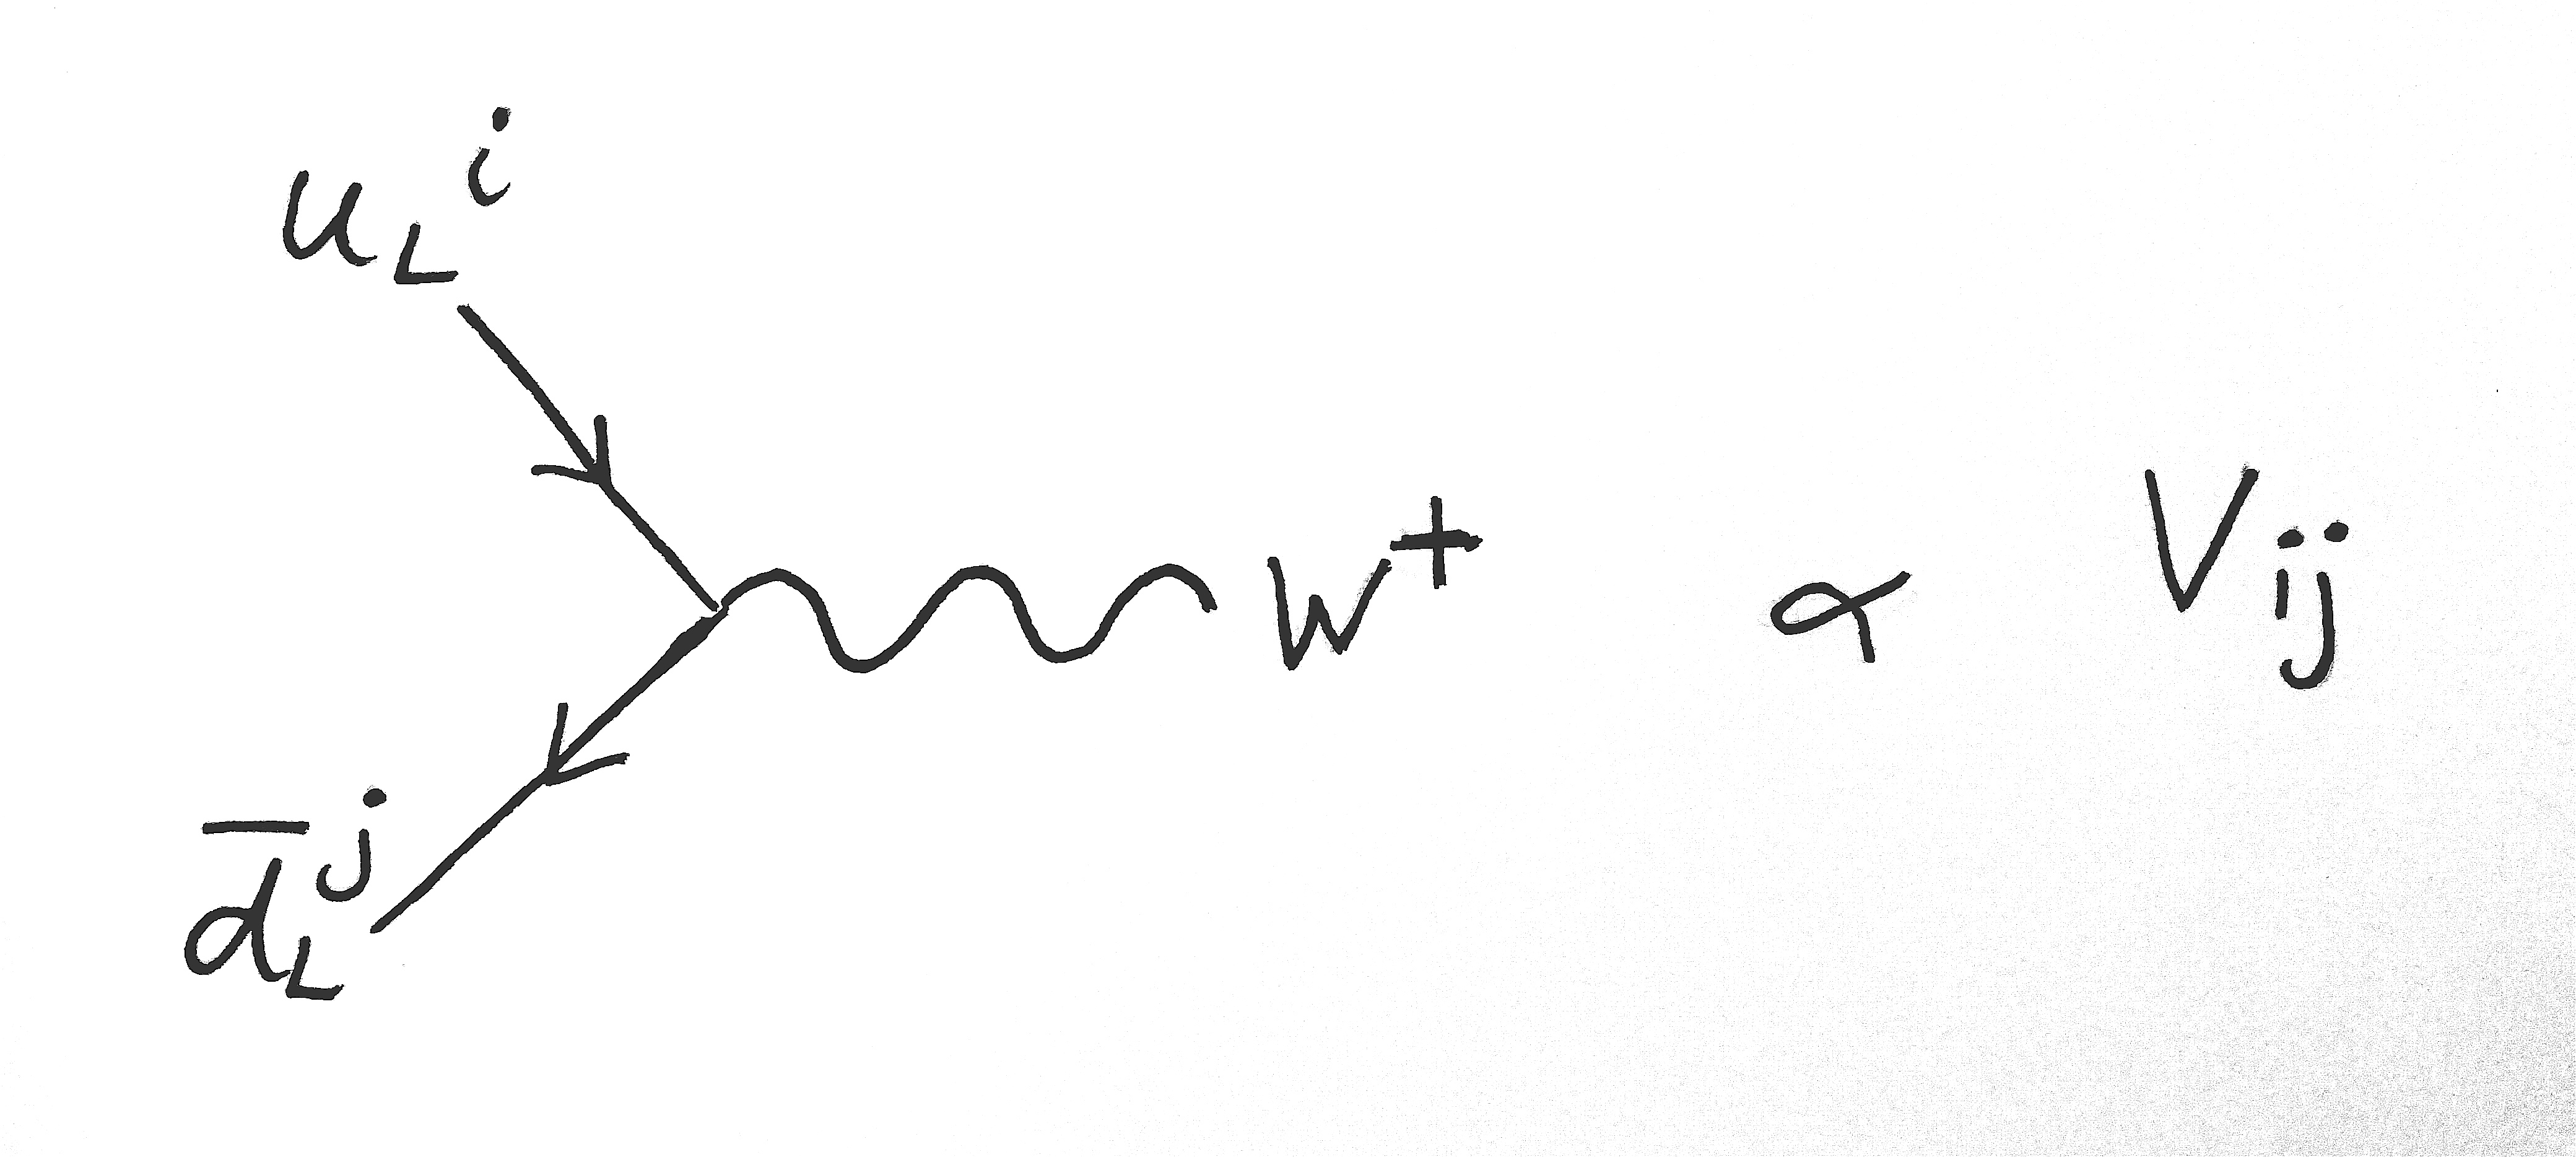
\includegraphics[width=0.5\textwidth]{images/fccc.jpg}
    \vspace{-10pt}
  \end{center}
  \caption{The flavour-changing charged current vertex.}
  \label{fig:fccc}
\end{figure}

\subsection{The CKM Matrix}

The exact values of the CKM matrix elements are of interest in the search for new physics. The CKM matrix is unitary by construction, however, if we were to discover that the values we measure experimentally do not combine to produce a unitary matrix, this would be evidence that the elements we are measuring, in fact, compose a submatrix of a unitary matrix larger than $3\times 3$. This would imply the presence of further, heavier quark generations.

%% Another source of interest in the CKM values is CP violation. CP violation is a global symmetry exhibited by $\mathcal{L}_{\text{SM}}-\mathcal{L}_{\text{FCCC}}$, and physically corresponds to a symmetry between particles and antiparticles. CP violation is one of the famous {\it{Sakarov conditions}}, the conditions necessary for a theory to explain the matter/antimatter asymmetry observed in the universe. CP is generically violated when a parameter of the theory has an imaginary component. The CKM matrix contains one physical phase, making $\mathcal{L}_{\text{FCCC}}$ a source of CP violation. However, the extent of CP violation in the flavour sector is not sufficient to explain the matter/antimatter asymmetry, so the necessary CP violating processes will likely come from new physics beyond the standard model.


%% To understand the structure of the CKM, we must first ask how many independent physical parameters there are. If one imagines that $V$ is purely real, then it becomes an $SO(3)$ matrix, which can be parameterised by 3 angles, so there are $N_{\text{real}} = 3$ independent real parameters. A member of $SU(3)$ has 9 independent parameters, so there must be $N_{\text{im}}=N-N_{\text{real}} = 6$ independent phases.

%% However, we have the freedom to remove some of those phases via a redefinition of the quark fields. $\mathcal{L}_{\text{SM}} - \mathcal{L}_{\text{FCCC}}$ has a global $U(1)^6$ symmetry, a rephasing of each of the 6 quark flavours. One can rephase each flavour without modifying $\mathcal{L}_{\text{SM}} - \mathcal{L}_{\text{FCCC}}$, but with the effect of changing $V$:
%% \begin{align}
%%   V \,\,\to \,\,
%%   \begin{pmatrix}
%%     e^{-ia} & 0 & 0 \\
%%     0 & e^{-ib} & 0 \\
%%     0 & 0 & e^{-ic} \\
%%   \end{pmatrix}
%%   V
%%   \begin{pmatrix}
%%     e^{id} & 0 & 0 \\
%%     0 & e^{ie} & 0 \\
%%     0 & 0 & e^{if} \\
%%   \end{pmatrix},
%% \end{align}
%% where $a,b,c,d,e,f\in \mathbb{R}$. So perhaps one can tune each of these 6 phases to remove all 6 phases in $V$. This is not quite right, we in fact only have the ability to remove 5 of the 6 phases. To see why we can redefine the phases in the following way;
%% \begin{align}
%%   V \,\,\to \,\,
%%   \begin{pmatrix}
%%     e^{-ia} & 0 & 0 \\
%%     0 & e^{-i(a+\alpha)} & 0 \\
%%     0 & 0 & e^{-i(a+\beta)} \\
%%   \end{pmatrix}
%%   V
%%   \begin{pmatrix}
%%     e^{i(a+\gamma)} & 0 & 0 \\
%%     0 & e^{i(a+\delta)} & 0 \\
%%     0 & 0 & e^{i(a+\epsilon)} \\
%%   \end{pmatrix},
%% \end{align}
%% with $\alpha,\beta,\gamma,\delta,\epsilon\in\mathbb{R}$. $a$ is a useless phase - it will always cancel with itself so cannot be used to remove a phase from $V$. Hence, one can remove 5 of the 6 phases by redefining the quark fields, leaving one physical phase in the CKM matrix.

%% This is can be seen as due to the explicit symmetry breaking property of $\mathcal{L}_{\text{FCCC}}$. The inclusion of $\mathcal{L}_{\text{FCCC}}$ breaks the global $U(1)^6$  symmetry down, $U(1)^6 \to U(1)$, where the broken symmetry is a rephasing of all of the quark flavours by the same amount. This says we can modify $\mathcal{L}_{\text{FCCC}}$ by $N_{\text{broken}} = 5$ independent phases without modifying the rest of the Lagrangian.

The CKM contains 3 real parameters and 1 complex phase. There is only one complex phase since we can freely redefine the phases of the quark fields in order to absorb the majority of the phases in the CKM. A common parameterisation is
\begin{align}
  V =
  \begin{pmatrix}
    1 & 0 & 0 \\
    0 & \cos\theta_{23} & \sin\theta_{23} \\
    0 & -\sin\theta_{23} & \cos\theta_{23} \\
  \end{pmatrix}
  \begin{pmatrix}
    1 & 0 & \sin\theta_{12}e^{i\delta} \\
    0 & 1 & 0  \\
    -\sin\theta_{13} e^{i\delta} & 0 & \cos\theta_{13} \\
  \end{pmatrix}
  \begin{pmatrix}
    \cos\theta_{12} & \sin\theta_{12} & 0  \\
    -\sin\theta_{12} & \cos\theta_{12} & 0 \\
    0 & 0 & 1 \\
  \end{pmatrix}.
\end{align}
A useful parameterisation for understanding the relative sizes of the CKM elements is due to Wolfenstein. Define the Wolfenstein parameter $\lambda = \sin\theta_{12}$, which is known experimentally to be around $\lambda\simeq 0.22$. Then $\cos\theta_{12} = \sqrt{1-\sin^2\theta_{12}} = \sqrt{1-\theta^2} \simeq 1 - \lambda^2/2$. Observing then that $\sin\theta_{23} \sim 0.04 \simeq \lambda^2$ and $\sin\theta_{13} \sim 0.004 \simeq \lambda^3/3$, we can write the matrix as
\begin{align}
  V \simeq
  \begin{pmatrix}
    1 - {1\over 2}\lambda^2 & \lambda & {1\over 3} \lambda^3 e^{i\delta}  \\
    - \lambda & 1 - {1\over 2}\lambda^2 & \lambda^2 \\
    \lambda^3(1-{1\over3} e^{i\delta}) & -\lambda^2 & 1 \\
  \end{pmatrix}
  =
  \begin{pmatrix}
    \order{1} & \order{\lambda} & \order{\lambda^3}  \\
    \order{\lambda} & \order{1} & \order{\lambda^2} \\
    \order{\lambda^3} & \order{\lambda^2} & \order{1} \\
  \end{pmatrix}
\end{align}
There is a clear hierarchy between the values - the CKM matrix is close to the unit matrix. Inter-generational mixing is dominant, dropping from second to first generation is suppressed by $\lambda$, dropping from third to second by $\lambda^2$, and dropping from third to first by $\lambda^3$. The SM supplies no compelling explaination of why this hierarchy exists, it is expected that new physics beyond the SM will supply some natural explaination.

The assumption of unitarity in $V$,
\begin{align}
  V_{ji}^*V_{jk}=\delta_{ik},
  \label{eq:CKMunitarity}
\end{align}
imposes 9 constraints on the CKM elements. Each of these constraints gives a test of the SM, if one of these constraints is found to be violated, this represents evidence of new phyisics. The most studied constraint is given by taking $i=3,k=1$;
\begin{align}
  {V_{ud}V_{ub}^*\over V_{cd} V_{cb}^*} + {V_{td}V_{tb}^* \over V_{cd}V_{cb}^*} + 1 = 0.
\end{align}
This can be visualized as a triangle (known as the {\it{unitarity triangle}}) on the complex plane, as shown in figure \ref{fig:unitaritytriangle_sketch}.

\begin{figure}
  \vspace{-10pt}
  \begin{center}
    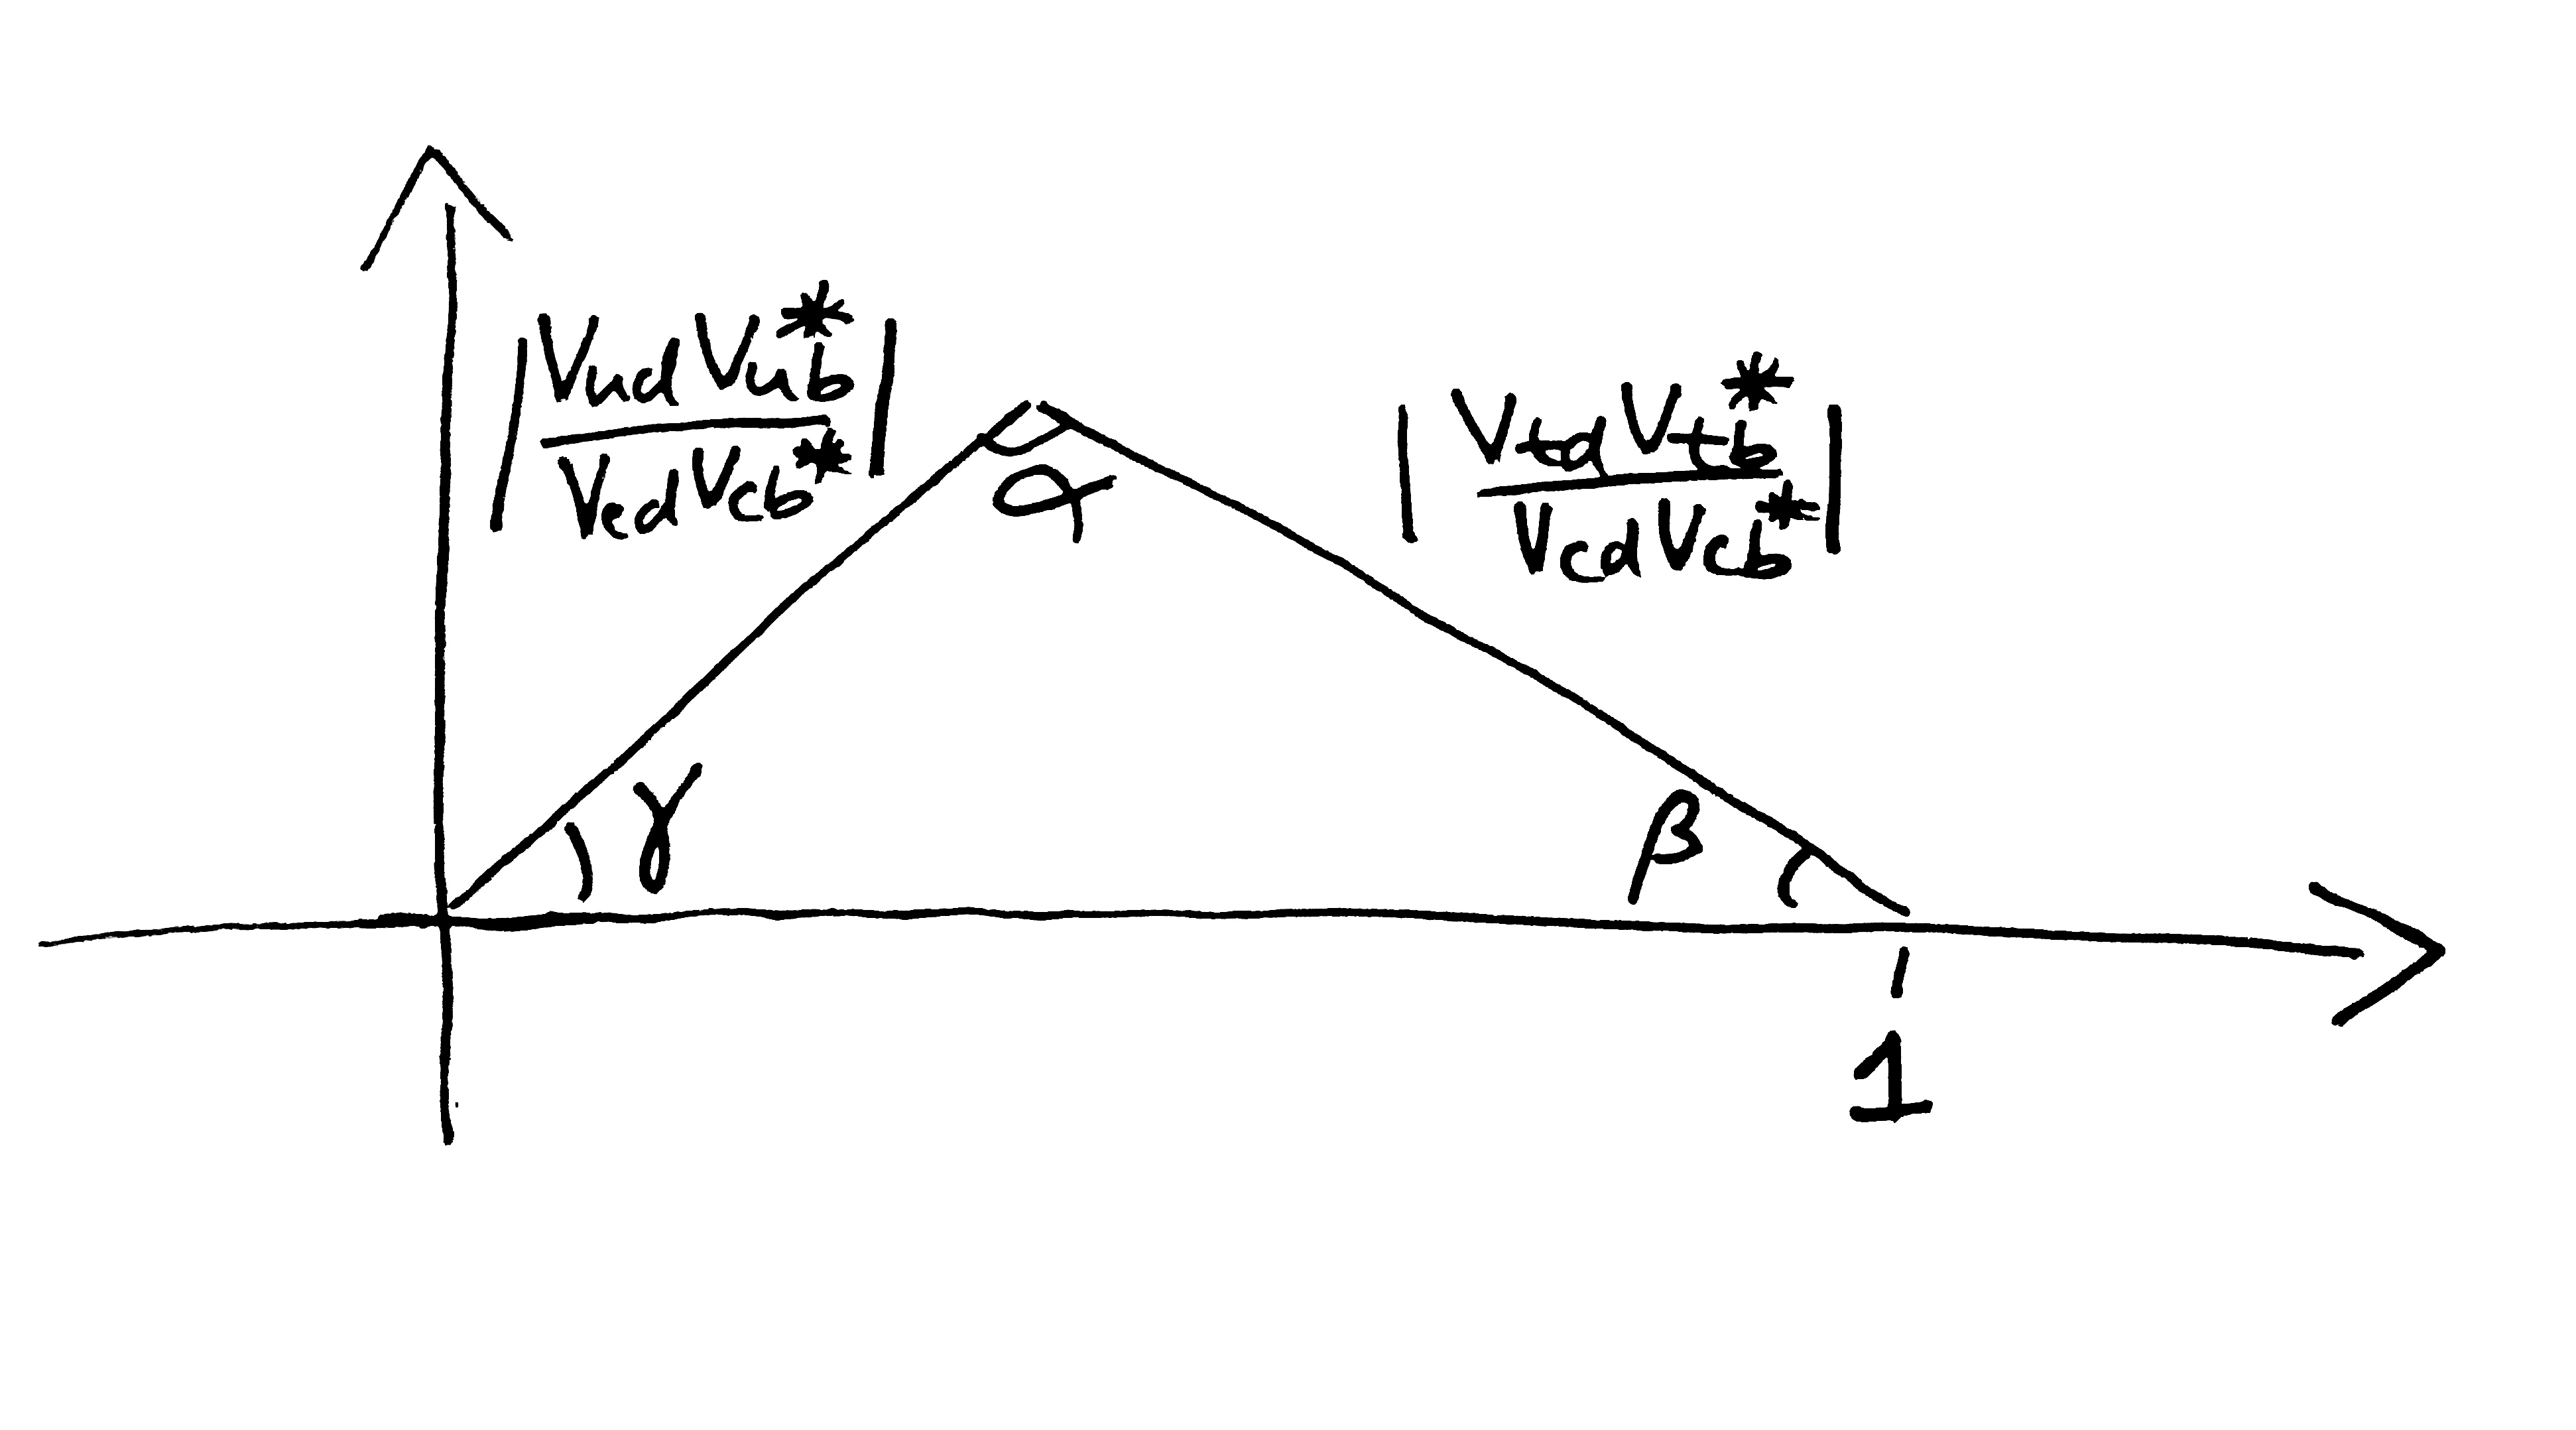
\includegraphics[width=0.7\textwidth]{images/unitaritytriangle_sketch.jpg}
  \end{center}
  \vspace{-40pt}
  \caption{A sketch of the unitarity triangle.}
  \label{fig:unitaritytriangle_sketch}
\end{figure}

For unitarity, the triangle must close, in other words, $\alpha+\beta+\gamma = \pi/2$. Hence to test the CKM unitarity experimentalists measure these angles
\begin{align}
  \alpha = \arg \left( -{V_{td}V_{tb}^*\over V_{ud}V_{ub}^*}\right) \,,\,
  \beta = \arg \left( -{V_{cd}V_{cb}^*\over V_{td}V_{tb}^*} \right) \,,\,
  \gamma = \arg \left( -{V_{ud}V_{ub}^*\over V_{cd}V_{cb}^*} \right).
\end{align}
The unitarity triangle also contains information about CP-violation from flavour-changing charged currents. The so-called Jarlskog invariant, $J=\sin\theta_{12}\sin\theta_{23}\sin\theta_{31}\cos\theta_{12}\cos\theta_{23}\cos\theta_{31}^2\sin\delta$, a measure of CP-violation, is proportional to the area enclosed by the triangle.

The most recent PDG update \cite{PhysRevD.98.030001} reports the following averages for the measurements of CKM elements;
\begin{align}
  |V| = \begin{pmatrix}
    0.97446\pm 0.00010 & 0.22452\pm 0.00044 & 0.00365\pm 0.00012 \\
    0.22438\pm 0.00044 & 0.97359\substack{+0.00010\\-0.00011} & 0.04214\pm 0.00076 \\
    0.00896\substack{+0.00024\\-0.00023} & 0.04133\pm 0.00074 & 0.999105\pm 0.000032 \\
  \end{pmatrix}.
\end{align}
The averages given here are consistent with unitarity in all avaliable tests. %For example, taking \eqref{eq:CKMunitarity} with $i=k=1$, we find $|V_{ud}|^2+|V_{us}|^2+|V_{ub}|^2 = 0.9994\pm 0.0005$.
The angles of the unitarity triangle currently satisfy $\alpha+\beta+\gamma = (180\pm 7)\degree$. Increasing the precision of CKM determinations are necessary to provide more stringent tests of CKM unitarity.

\begin{figure}
  \vspace{-10pt}
  \begin{center}
    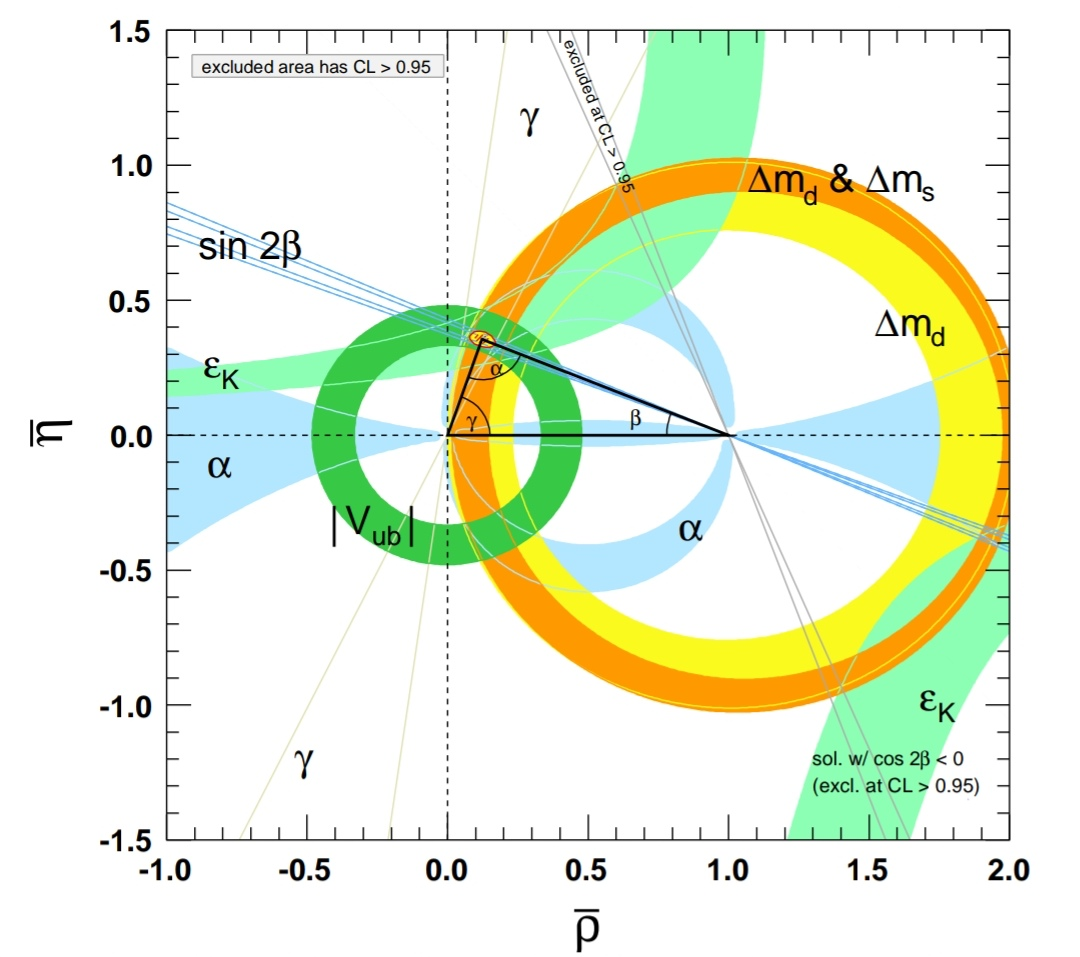
\includegraphics[width=0.6\textwidth]{images/ckmpdg.jpg}
  \end{center}
  \vspace{-25pt}
  \caption{Exclusion regions for the vertices of the CKM triangle from various measurements, coutresy of the most recent PDG update \cite{PhysRevD.98.030001}.}
  \label{fig:ckmpdg}
\end{figure}

\subsection{Weak Decays}
\label{sec:weakdecays}

We now move on to the methods of determining CKM elements. At the confinement scale ($\sim$1GeV and below), quarks are confined by QCD in hardons. At these energies, the dynamics of quarks are only experimentally accessible by probing the dynamics of hadrons. CKM matrix elements are determined by studying hadron decays.

First a word on hadrons. Hadrons are broadly categorized into mesons (charged with one valence quark and one valence antiquark) and baryons (three valence quarks). The entirety of this thesis is concerned with mesons. Mesons are categorized in terms of the flavours they are charged under and their representations under the Lorentz group. We use the same notation as for the quantum numbers of the weak currents; $L^{\pm}$ where $L$ denotes spin and $\pm$ denotes parity. In this thesis, we are concerned mostly with pseudoscalar ($0^-$) and vector ($1^-$) mesons.

Weak decays of mesons are categorized according to the final products:
\begin{itemize}
\item
  {\bf{Leptonic}}: $meson \to leptons$.
\item
  {\bf{Semileptonic}}: $meson \to meson + leptons$.
\item
  {\bf{Hadronic}}: $meson \to mesons$.
\item
  {\bf{Oscillation}}: $meson \to meson$.
\end{itemize}

All of these types of decay are dependent on CKM elements so can in principle to be used for studying them. We are most interested in the first two, leptonic and semileptonic, so will give detail of such decays here.

\begin{figure}
  \vspace{-10pt}
  \begin{center}
    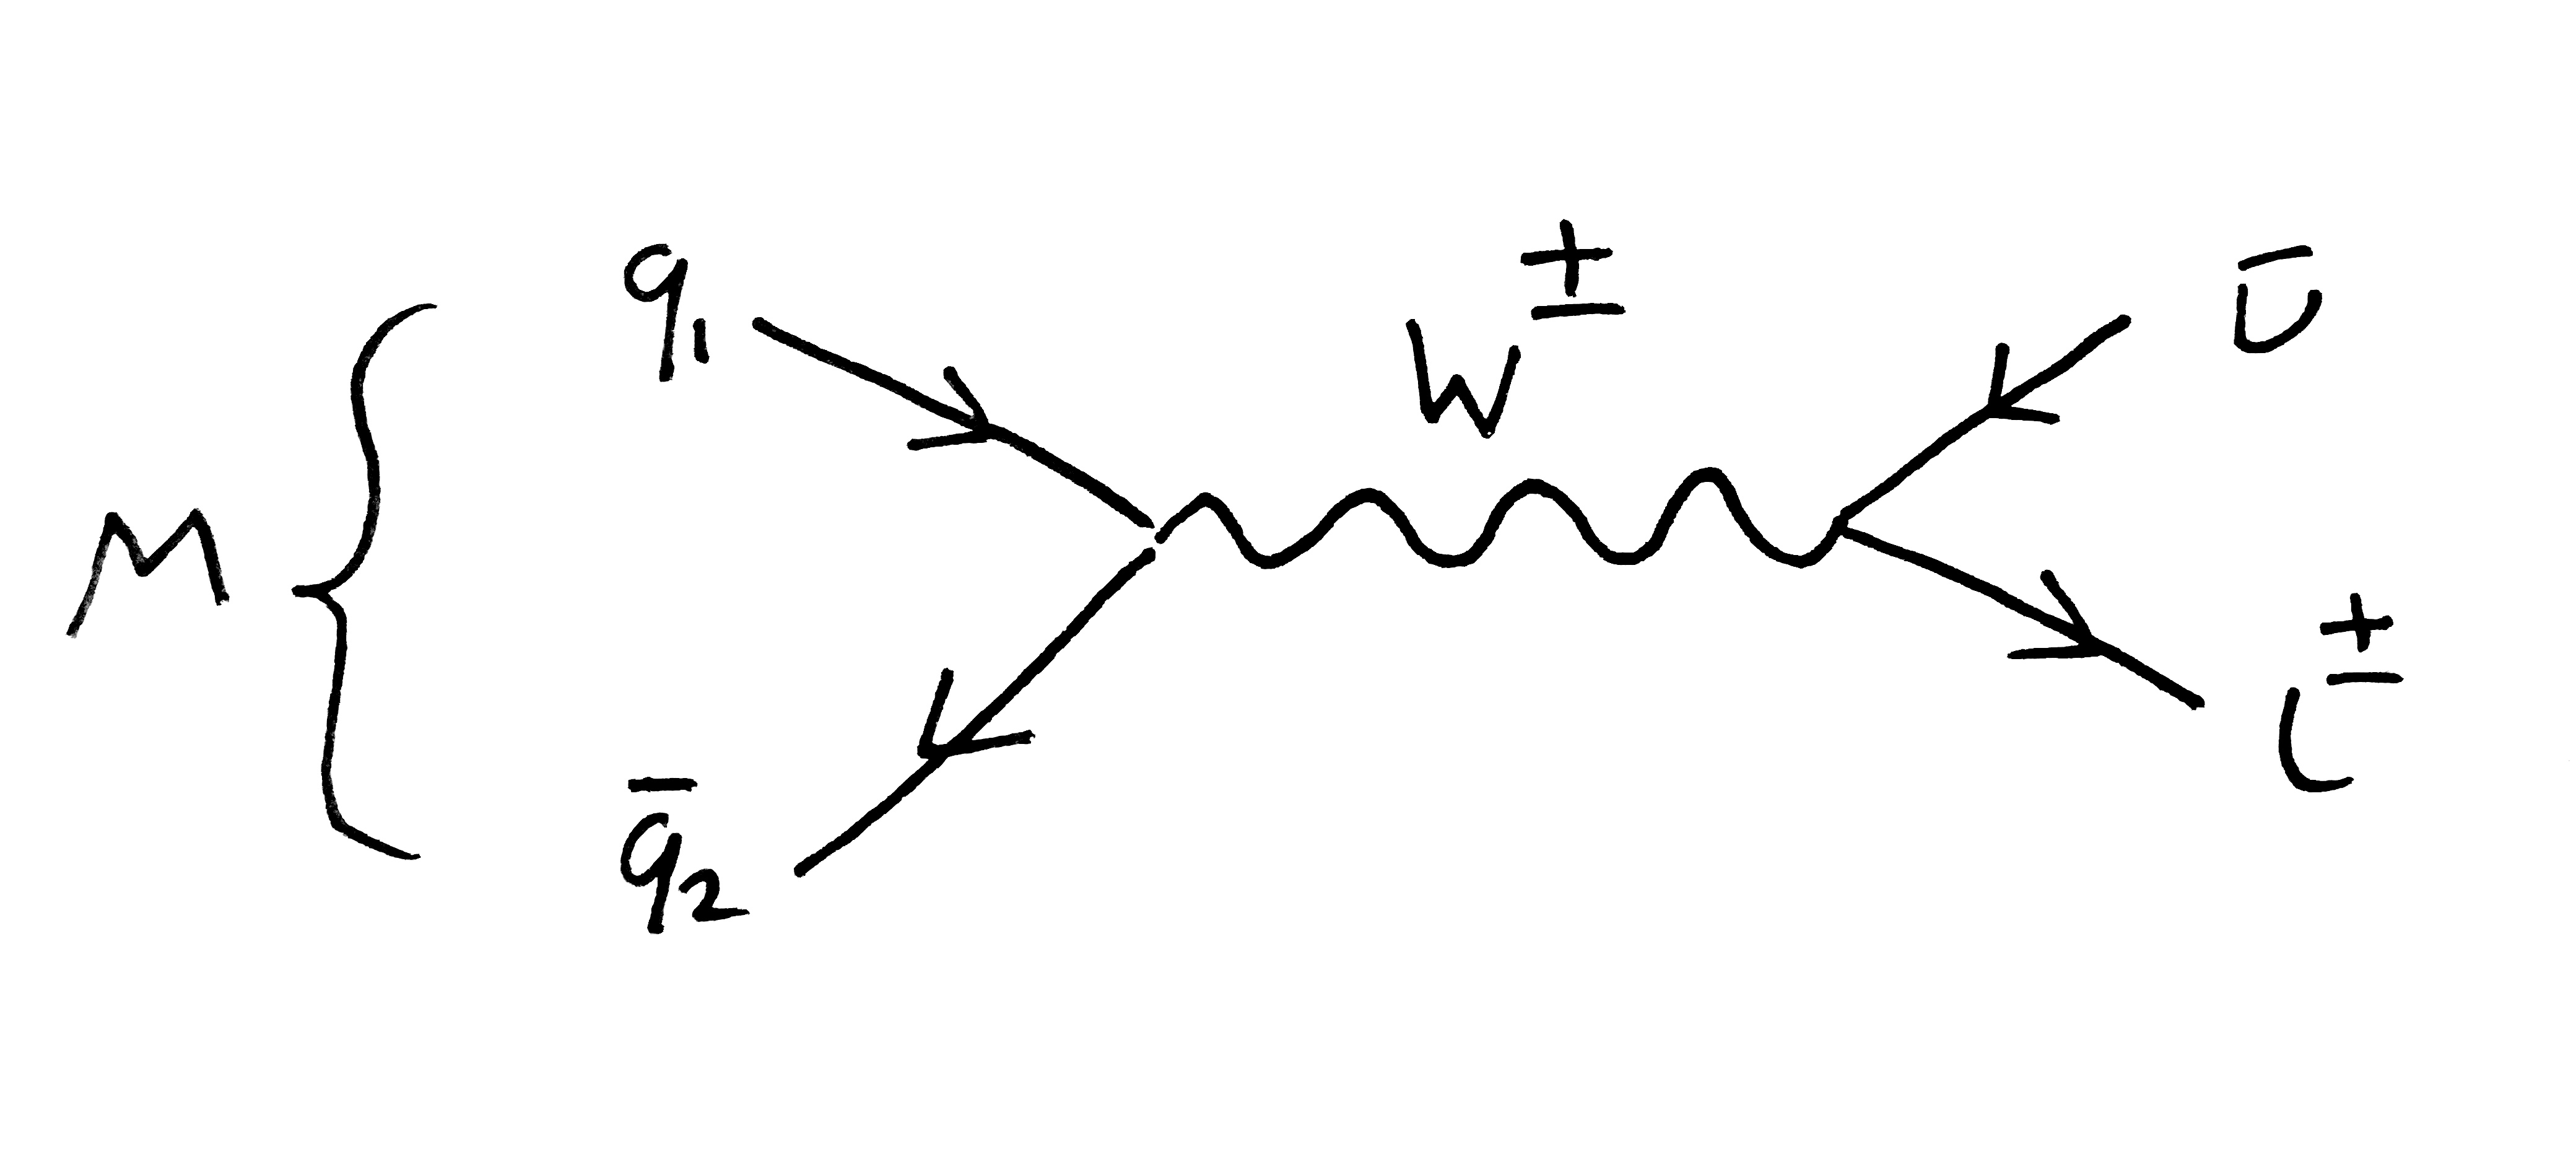
\includegraphics[width=0.6\textwidth]{images/leptonicdecay.jpg}
  \end{center}
  \vspace{-20pt}
  \caption{Leptonic decay of meson $M$ at tree level in the electroweak coupling.}
  \label{fig:leptonicdecay}
\end{figure}

Fig. \ref{fig:leptonicdecay} shows a generic leptonic decay at tree level (in electroweak coupling, virtual quark and gluon lines are implicit). The corresponding amplitude is given by
\begin{align}
  \mathcal{M} = \left({ie\over \sqrt{2}\sin\theta_W}\right) V_{q_1q_2} \langle l\bar{\nu} | L^l_{\mu} D_W^{\mu\nu} J_{\nu}^{q_1q_2} | M \rangle,
\end{align}
where $D_{W}$ is a free $W^{+-}$ propagator, $|M\rangle$ is the ground state of the meson $M$, and $|l\bar{\nu}\rangle$ is a lepton-antineutrino state. We are using the notation $L^l_{\mu}=L^{kk}_{\mu}$, where $l$ indexes the $k$th charged lepton. If the momentum of the meson, $p^2$, is much smaller than the $W$ mass squared, one can integrate out the dynamics of the $W$ to move into the Fermi effective theory \cite{Borasoy:2007yi};
\begin{align}
  \nonumber
  \left({ie\over\sqrt{2}\sin\theta_W}\right)^2 D^{\mu\nu}_W(p^2) &= \left({ie\over\sqrt{2}\sin\theta_W}\right)^2 \left( -ig^{\mu\nu} \over p^2 - M_W^2 \right)
  \\ & = \underbrace{ {i\over M_W^2} \left( ie \over \sqrt{2}\sin\theta_W \right)^2  }_{\equiv -2\sqrt{2}G_F} g^{\mu\nu} + \mathcal{O}\left({p^2\over M_W^4}\right).
\end{align}
Then $\mathcal{M}$ can be factorised;
\begin{align}
  \mathcal{M} \simeq -2\sqrt{2} V_{q_1q_2} \langle l\bar{\nu} | L_{\mu}^l | \Omega \rangle \langle \Omega | J^{q_1q_2\, \mu} | M \rangle.
\end{align}
$\langle \Omega | J^{q_1q_2}_{\mu}| M \rangle$ is a non-perturbative quantity, since it concerns the transitions of a strongly coupled bound state (QCD at the confinement scale). We know that it has a lorentz index $\mu$, and the only Lorentz vector in the system is the meson's 4-momentum $p_{\mu}$. So we define
\begin{align}
  \langle\Omega | J_{q_1q_2}^{\mu} | M \rangle = p^{\mu} f_M,
  \label{eq:decay_constant_def}
\end{align}
where $f_M$ is a Lorentz invariant known as the {\it{decay constant}} of the meson $M$, and encodes all non-perturbative information in the amplitude.

By taking the modulus squared of $\mathcal{M}$, and integrating over all allowed momenta of the final state, one finds the decay rate of the process;
\begin{align}
  \Gamma(M\to l\bar{\nu}) = {G_F^2\over 8\pi} f_M^2 m_l^2 M_M \left( 1 - {m_l\over M_M^2} \right)^2 |V_{q_1q_2}|^2,
\end{align}
In order to find $|V_{q_1q_2}|$, one requires both a measurement of $\Gamma(M\to l\bar{\nu})$, and a value for $f_M$. $f_M$ can be computed in a Lattice QCD calculation.

%\begin{wrapfigure}{R}{0.55\textwidth}
\begin{figure}
  \vspace{-10pt}
  \begin{center}
    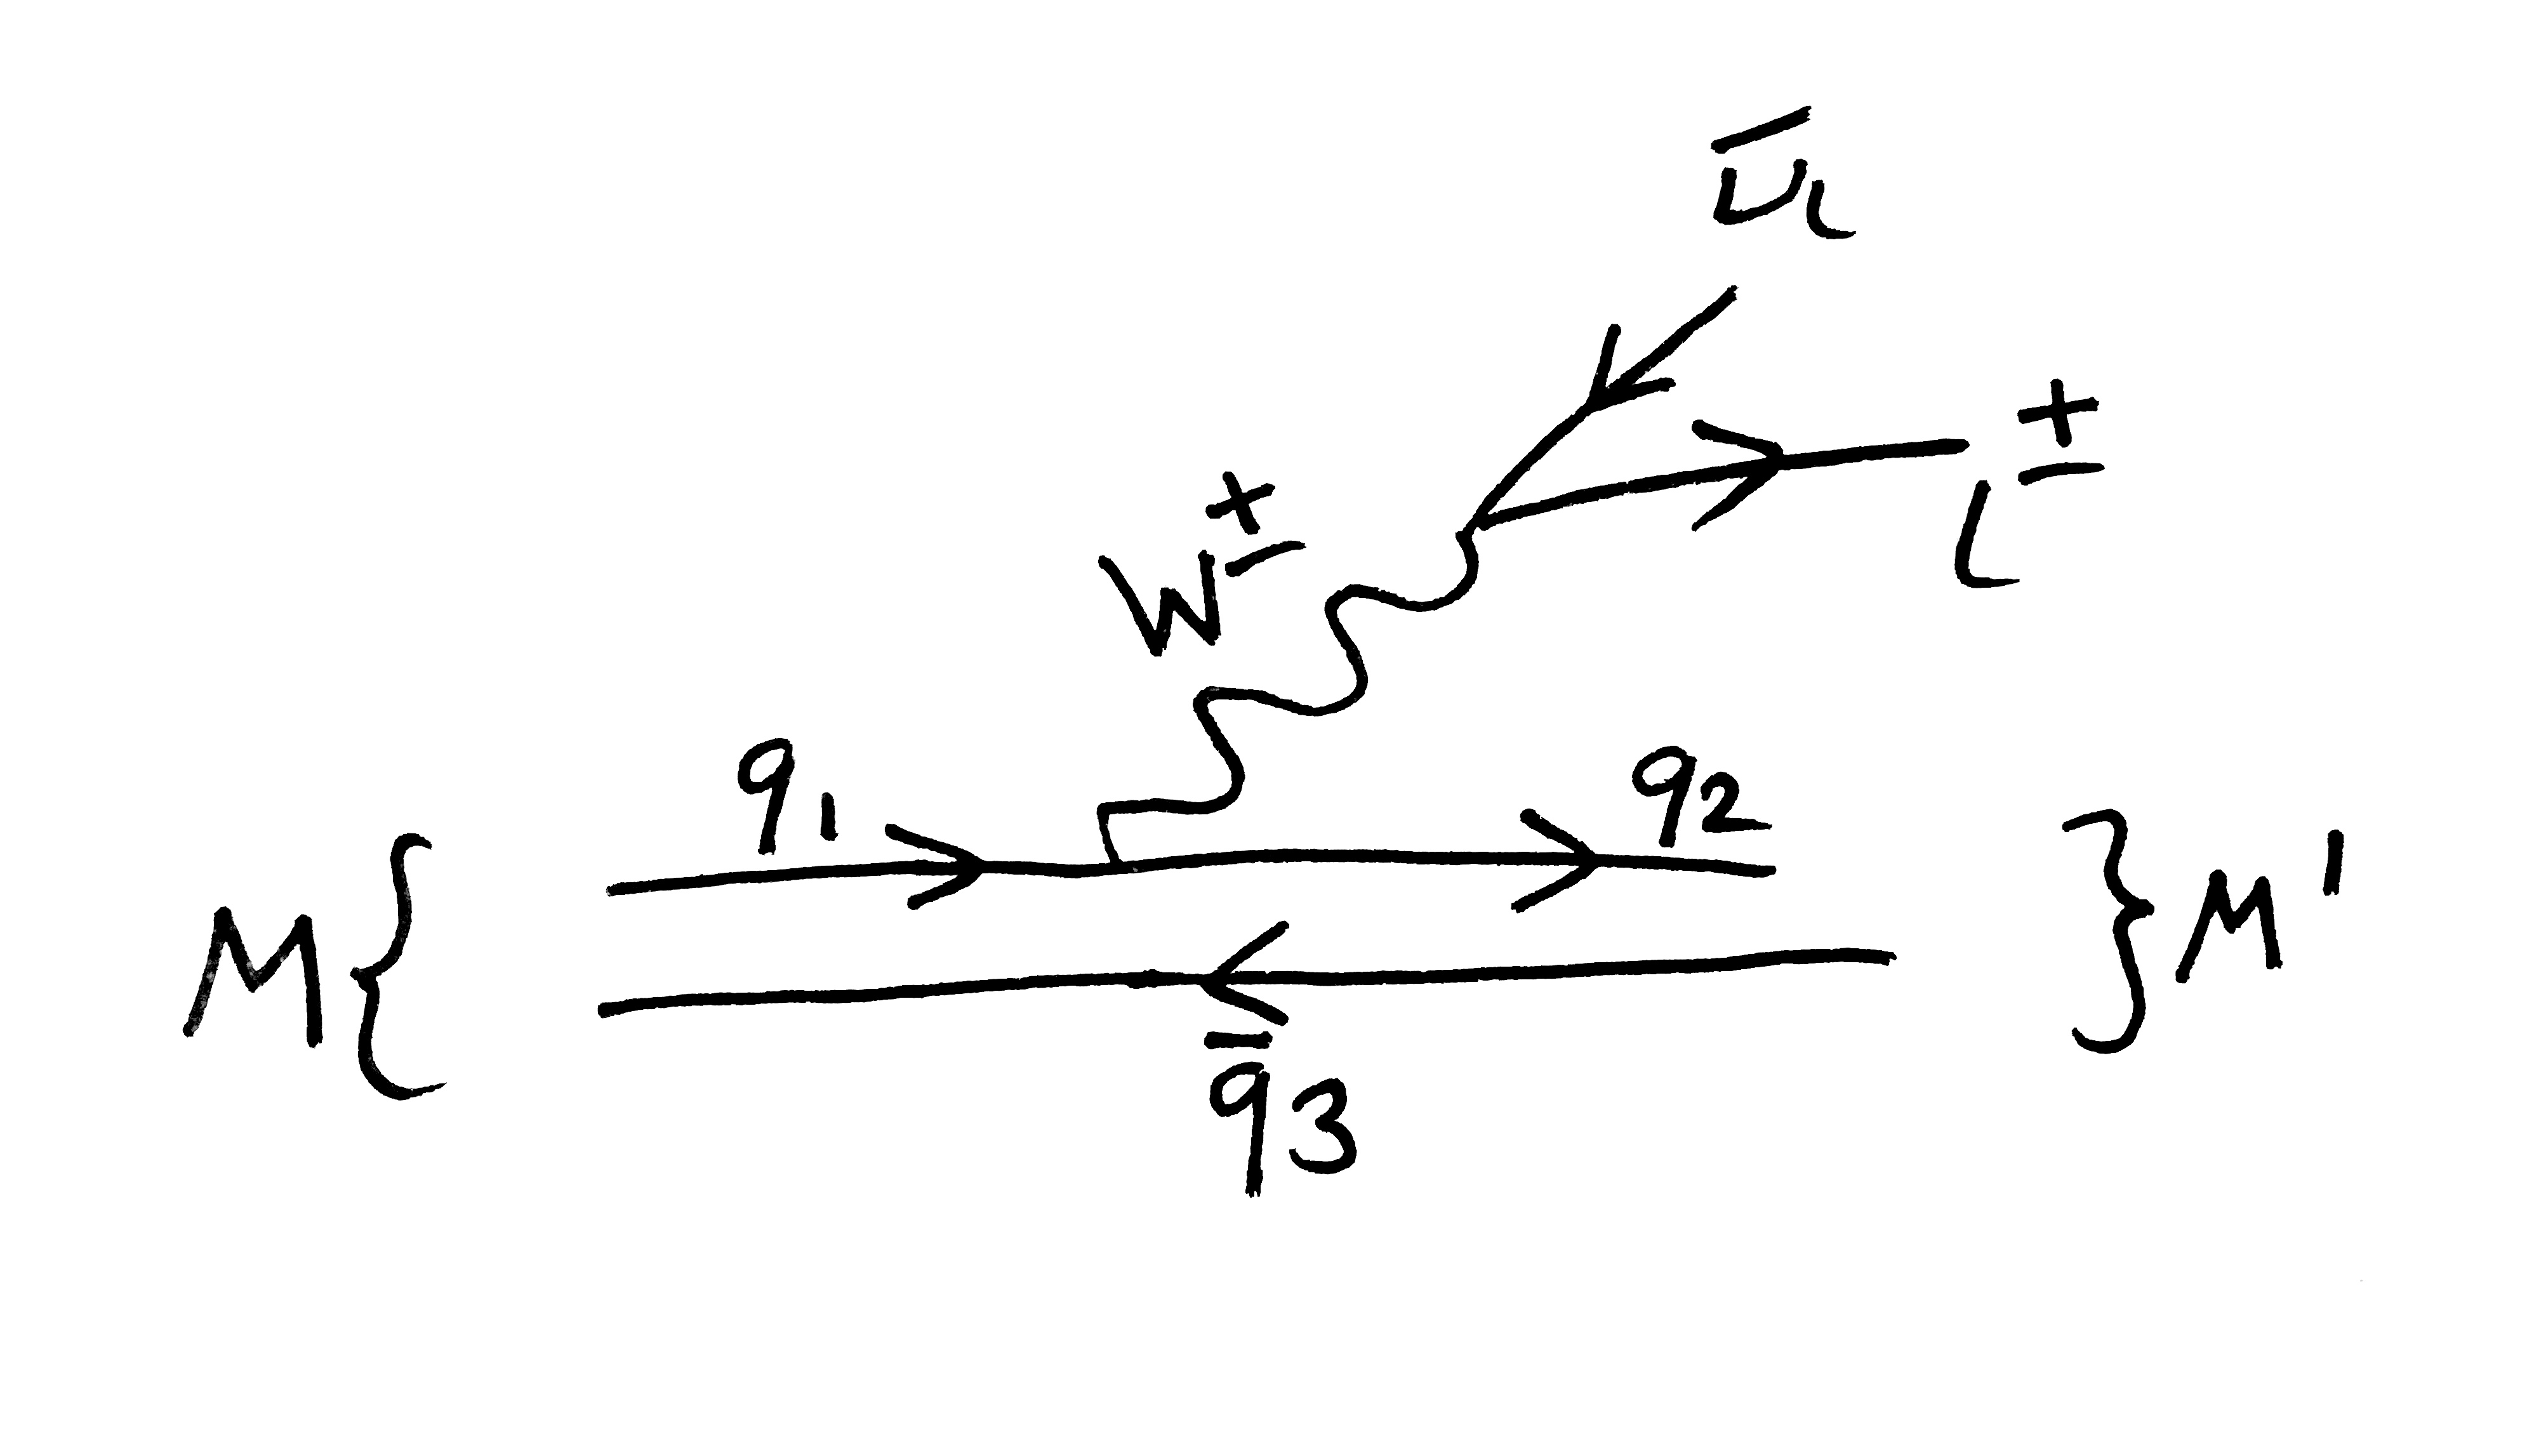
\includegraphics[width=0.6\textwidth]{images/semileptonicdecay.jpg}
  \end{center}
  \vspace{-30pt}
  \caption{Semileptonic decay, $M\to M'l\bar{\nu}$, at tree level in electroweak coupling.}
  \label{fig:semileptonicdecay}
\end{figure}
%\end{wrapfigure}

A similar story accompanies semileptonic decays. At tree level in the electroweak coupling, a typical semileptonic decay is depicted in fig. \ref{fig:semileptonic}. The amplitude is given by
\begin{align}
  \nonumber
  \mathcal{M} & = \left( { ie \over \sqrt{2} \sin\theta_W }\right) V_{q_1q_2} \langle M', l\bar{\nu} | J_{\mu}^{q_1q_2} D_W^{\mu\nu} L^l_{\nu} | M \rangle \\
  \nonumber
  & \simeq -2\sqrt{2} G_F V_{q_1q_2} \langle M', l\bar{\nu} | J_{\mu}^{q_1q_2} L^{l\, \mu} | M \rangle \\
  & \simeq -2\sqrt{2} G_F V_{q_1q_2} \langle l\bar{\nu} | L^{l\,\mu} | \Omega \rangle \langle M' | J_{\mu}^{q_1q_2} | M \rangle,
  \label{eq:semileptonic}
\end{align}
where on the second line we have integrated out the $W$ propagator in using the same expansion as in the leptonic case, and on the third line we have factorised the QCD part from the electroweak part. The matrix element $\langle M' | J_{\mu}^{q_1q_2} | M \rangle$ is a non-perturbative quantity. Unlike in the previous case, there are a number of ways one can choose to parameterise this matrix element, and appropriate choices vary depending on the quantum numbers of $M$ and $M'$. Of interest to us are the cases where $M$ is a pseudoscalar meson $0^-$, and $M'$ is either pseudoscalar or vector $1^-$.

In the {\bf{pseudoscalar$\to$pseudoscalar}} case, only the vector component of the current survives in the matrix element, $\langle M' | J_{\mu}^{q_1q_2} | M \rangle = \langle M' | V_{\mu}^{q_1q_2} | M \rangle$. $\,\,\langle M' | A_{\mu}^{q_1q_2} | M \rangle$ vanishes since this does not respect the parity invariance of QCD. The most popular parameterisation of $\langle M' | V_{\mu}^{q_1q_2} | M \rangle$ is
\begin{align}
  \langle M' | V_{\mu}^{q_1q_2} | M \rangle = f_+(q^2) \left[ P_{\mu} + p_{\mu} - {M^2-m^2\over q^2} q_{\mu} \right]  + f_0(q^2) {M^2-m^2\over q^2} q_{\mu}.
  \label{eq:formfactors_experimental}
\end{align}
$M,P_{\mu}$ are the $M$-meson mass and momentum, $m,p_{\mu}$ are the$M'$-meson mass and momentum. $f_0(q^2)$ and $f_+(q^2)$, known as the scalar and vector form factors, encoding all non-perturbative information. We now have non-perturbative functions of $q^2$ rather than a single number. $q^2=(P-p)^2$, the momentum carried away from the meson by the $W$, has an allowed range of values if the final states are on-shell;
\begin{align}
  m_l^2 \leq q^2 \leq (M-m)^2.
\end{align}
By integrating $|\mathcal{M}|^2$ over all final lepton and neutrino momenta, one finds a differential decay rate,
\begin{align}
  {d\Gamma\over dq^2}(M\to M'l\bar{\nu}) =& \eta_{\text{EW}} { G_F^2 |V_{q_1q_2}|^2\over 24 \pi^3 M^2 } \left( 1 - {m_l^2\over q^2}\right)^2 |{\bf{p}}| \,\,\times \\
  \label{eq:branchingfraction}
  &\left[ \left( 1 + {m_l^2\over 2q^2}\right) M^2 |{\bf{p}}|^2 f_+^2(q^2) + {3m_l^2\over 8q^2} (M^2-m^2)^2 f_0^2(q^2) \right]. \nonumber
\end{align}
${\eta}_{\text{EW}}$ accounts for electroweak corrections due to diagrams where photons or $Z$s are exchanged in addition to a $W^-$, as well as the Coulomb attraction of the final-state charged particles \cite{SIRLIN198283,Ginsberg1968,PhysRevD.41.1736}. ${\bf{p}}$ is the final meson state ($M'$) spacial momentum. Once again, to deduce $|V_{q_1q_2}|$, one requires both the decay rates $d\Gamma/dq^2$, and the form factors $f_0(q^2)$,$f_+(q^2)$. To precisely determine the form factors requires a Lattice QCD calculation.

In the {\bf{pseudoscalar$\to$vector}} case, both the vector and axial-vector components of the current survive in the matrix element. A common choice of parameterisation is
%% \begin{align}
%%   \langle M' | V^{\mu} | M \rangle &= {2iV(q^2)\over M+m} \epsilon^{\mu\nu\rho\sigma} \epsilon_{\nu}^* p_{\rho}P_{\sigma} \\
%%   \langle M' | A^{\mu} | M \rangle &= 2mA_0(q^2) {\epsilon^*\cdot q\over q^2} q^{\mu} + (M+m)A_1(q^2)\left[ \epsilon^{*\,\mu} - {\epsilon^*\cdot q\over q^2} q^{\mu} \right] \\
%%   \nonumber
%%   &- A_2(q^2) {\epsilon^*\cdot q\over M + m} \left[ P^{\mu} + p^{\mu} - {M^2-m^2\over q^2} q^{\mu} \right].
%% \end{align}
\begin{align}
  \langle M'(\epsilon)| V_{q_1q_2}^{\mu} | M \rangle &= i \sqrt{Mm}\, h^s_V(w) \epsilon_{\mu\nu\alpha\beta} \,\epsilon^{*\nu} v'^{\alpha} v^{\beta}, \\
  \langle M'(\epsilon)| A_{q_1q_2}^{\mu} | M \rangle &= \sqrt{Mm} \, [ h^s_{A_1}(w) (w+1) \epsilon^*_{\mu} - \\ \nonumber
    h^s_{A_2}(w)& \,\epsilon^*\cdot v \,v_{\mu} - h^s_{A_3}(w) \,\epsilon^*\cdot v \, v'^{\mu} ].
\end{align}
$v = P/M$ and $v' = p/m$ are the 4-velocities of $M$ and $M'$ respectively. $\epsilon$ is the polarization of the vector meson $M'$. $w = v\cdot v'$ is known as the recoil parameter, this is an alternative to $q^2$ often used in heavy quark effective theory. $h_V(w),h_{A_0}(w),h_{A_1}(w)$, and $h_{A_2}(w)$ are the form factors accounting for the non-perturbative physics. The decay rate is given by
\begin{align}
  {d\Gamma \over dw}(M\to M' l\bar{\nu}) = {G_F^2 m^3 | \eta_{\text{EW}} V_{q_1q_2} |^2 \over 4\pi^3 } (M-m)^2 \sqrt{w^2-1} \, \chi(w) |\mathcal{F}(w)|^2,
  \label{eq:pseudoscalar-vector-dr}
\end{align}
where $\mathcal{F}(w)$ is a linear combination of the form factors and $\chi(w)$ is a known function of $w$ (both given in e.g. appendix G of \cite{Harrison:2017fmw}).

At the zero recoil point, where $q^2$ is maximized at $q^2_{\text{max}} = (M-m)^2$, (correpsonding to $w=1$), a single form factor contributes
\begin{align}
  \mathcal{F}(1) = h_{A_1}(1).
\end{align}
However the differential decay rate vanishes at $w=1$. A common approach to determine $|V_{q_1q_2}|$, for example used to find $|V_{cb}|$ via the $B\to D^*l\bar{\nu}$ decay, is to find $|\mathcal{F}(1)V_{cb}|^2$ at zero recoil by extrapolating from experimental data at non-zero recoil, and combining this with a lattice QCD determination of $h_{A_1}(1)$.

\subsection{$b\to c$ Transitions and $|V_{cb}|$}

The family of weak decays that have attracted the most attention are decays of $B$ mesons (pseudoscalar mesons containing a valence $b$ and $u,d,s$ or $c$ quark). $B$ mesons decay into a rich variety of decay products. It is the heaviest quark flavour that can be found in hadrons (the only heavier quark, the top quark, has a mass far above the confinement scale, so does not feature as a valence quark in hadrons).

The $b$ can decay into either a $c$ or a $u$ quark via the flavour changing charged current. In this thesis we are interested in the $b\to c$ transition, with an amplitude proportional to the CKM element $|V_{cb}|$. In this section, we give a brief overview of how this is calculated and the value's current status.

$B$ meson decays can be measured in a number of experiments. There are two so-called $b$-factories, the Belle (II) experiment at the KEKB collider in Japan, and the BaBar experiment at the PEP-II collider at SLAC laboratory in the US. These are $e^+e^-$ colliders, that collide with an energy tuned to the mass of the $\Upsilon(4s)$, an excited state of the $\Upsilon$ meson (a $1^-$ state with $\bar{b}b$ valence quarks). The $\Upsilon(4s)$ has a large branching fraction into a $B\bar{B}$ pair, the decays of these can be measured with large statistics. $B$ decays can also be measured in proton colliders, like at the LHCb experiment at CERN. Measurements from LHCb have poorer statistics but cover a larger range of the phase space of final states, due to the variance of momenta in the initial state protons.

So far 3 approaches to determining $|V_{cb}|$ have been carried out:
\begin{itemize}
\item
  $B\to D^* l\bar{\nu}$ decay rate measurements are extrapolated to zero recoil to determine $|V_{cb}h_{A_1}(1)|$. Then dividing out $h_{A_1}(1)$ from a Lattice calculation, one finds $|V_{cb}|$.
\item
  $B\to D l\bar{\nu}$ decay rates are measured throughout $q^2$, and combined with $f_0(q^2)$ and $f_+(q^2)$ from lattice calculations.
\item
  $B\to X_c l\bar{\nu}$ decay rates are measured (where $X_c$ is all possible charmed final state mesons), this is used to constrain elements in the operator product expansion, a method first devised in \cite{Bigi:1996si,Hoang:1998hm}.
\end{itemize}
The first two are referred to as {\it{exclusive}} and the third {\it{inclusive}}. A selection of the most accurate examples of each method of determination is given in figure \ref{fig:Vcb_plot}.
\begin{figure}
  \vspace{-10pt}
  \begin{center}
    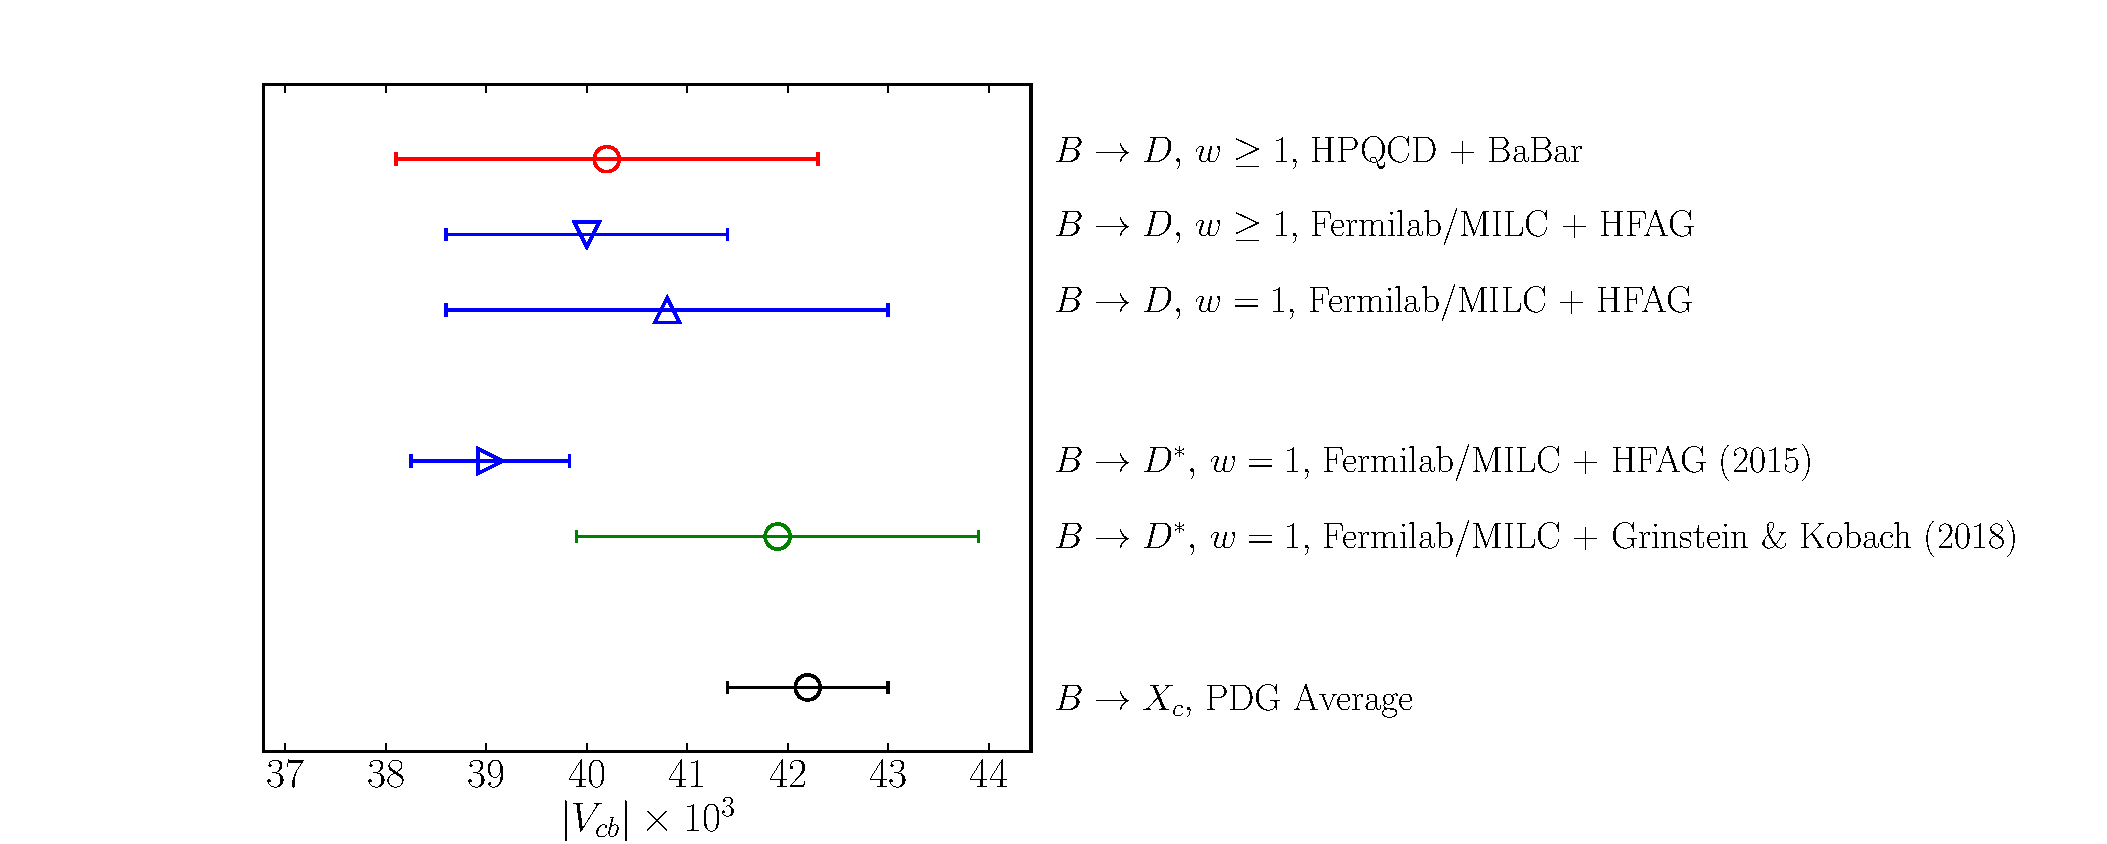
\includegraphics[width=1.0\textwidth]{images/Vcb_plot.pdf}
  \end{center}
  \vspace{-20pt}
  \caption{Different determinations of $|V_{cb}|$. Points labelled $w=1$ are determinations from extrapolating measurements of decay rates to the zero recoil point, and combining them with a lattice determination of the form factor at zero recoil. Points labelled $w\geq 1$ are results from using a combination of both branching fractions and lattice form factors through some range of $w$. The first name mentioned in the labels give the source of the lattice form factors, and the second gives the source of the experimental data (e.g. the HPQCD$+$BaBar point used form factors from the HPQCD collaboration and data from the BaBar experiment). The highest point is from \cite{Na:2015kha}, the second and third highest from \cite{Lattice:2015rga}, fourth from \cite{Bailey:2014tva}, fifth from \cite{Grinstein:2017nlq}. The bottom point is from the PDG \cite{PhysRevD.98.030001}, using data from the ALPEPH \cite{BUSKULIC1995236}, Belle \cite{Abe:2001yf}, BaBar \cite{Aubert:2008yv,Aubert:2009ac}, and CLEO \cite{Bartelt:1998dq} experiments.
    \label{fig:Vcb_plot}}
\end{figure}

This figure tells a story of the recent history of $|V_{cb}|$. Determinations from $B\to Dl\nu$ have been consistent but not as precise as via the other two methods. Until recently, there was a $3\sigma$ tension between determinations from the $B\to D^* l\nu$ decay and inclusive decays. This was on it's the way to being resolved when concern was raised about the method of extrapolating experimental data for $B\to D^*l\bar{\nu}$ decay rates to the zero recoil point ($w=1$).

The Heavy Flavour Averaging Group HFAG (Now HFLAV) determination of $|V_{cb}h_{A_1}(1)|$ in 2015 parameterised the form factors in the extrapolation using the CLN parameterisation (defined in section {\red{?}}). It has become clear that the constraints the CLN parameterisation imposes on the form factors are not justified. In \cite{Bigi:2017njr,Grinstein:2017nlq}, the results of an extrapolation using the CLN parameterisation were compared to results from a more general, model-independent parameterisation, the BGL parameterisation. It was found that they differed by $3.5\sigma$. Since the BGL makes fewer assumptions, one may consider this the more reliable result.

The $|V_{cb}|$ result using BGL to extrapolate the decay rates is given in the green point on fig. \ref{fig:Vcb_plot}. Hence, if this work is to be trusted, the long-standing $|V_{cb}|$ tension has been resolved.

There are however a number of other reasons to be interested in studying $|V_{cb}|$, namely improving its precision. It is currently the least precisely determined element of the CKM matrix. It constrains one side of the unitarity triangle via the ratio $|V_{ub}|/|V_{cb}|$, so it is the bottleneck for precise tests of CKM unitarity. It is also a dominant uncertainty in the determination of the $CP$-violation parameter $\epsilon_K$ (that is currently at tension between the SM and experiment, see for example \cite{Bailey:2018feb} where a $4\sigma$ tension is reported).

%% A dominant motivation for the work presented in this thesis is the quest for a more precise determination of $|V_{cb}|$. The main results are form factors for $B_s\to D_s l\bar{\nu}$ and $B_s\to D_s^* l\bar{\nu}$. The benefit of these determinations is two-fold. Firstly, they can be combined with future experimental measurements of $B_s\to D_s^{(*)}l\bar{\nu}$ decays for a new $|V_{cb}|$ determination. Increasing the number of independent determinations of $|V_{cb}|$ makes each result more robust. Secondly, they demonstrate that our approach in the lattice calculations work well and can, therefore, be applied to $B\to Dl\bar{\nu}$ and $B\to Dl\bar{\nu}$ form factors in the future.

\subsection{Flavour Anomalies \& Lepton Flavour Violation}

The SM can be tested by studying semileptonic decays more directly, without any consideration of CKM elements. CKM-independent observables can be constructed by taking ratios of branching fractions for decays with common CKM dependence. Then, form factors from lattice QCD can be used to form pure SM predictions of these ratios, and compared to purely experimental measurements. Such comparisons have uncovered a number of tensions between the SM and experiment.

The ratios are defined by
\begin{align}
  R_{X_q} = {\Gamma(B_q\to X_q \tau \nu_{\tau}) \over {1\over 2}\left[\Gamma(B_q\to X_q e \nu_e) + \Gamma(B_q\to X_q \mu \nu_{\mu}) \right]},
  \label{eq:Rratios}
\end{align}
where $X_q$ is any meson with valence quark content $x\bar{q}$. The numerator and denomenator will have the same power of $|V_{bx}|$, so cancel in the ratio.

There is currently tension between SM and experiment in $R_D$ and $R_{D^*}$.
\begin{gather}
  R_{D^*}|_{\text{exp}} = 0.306(13)_{\text{stat}}(07)_{\text{sys}}\quad,\quad R_{D^*}|_{\text{SM}} = 0.252(3)
  \\
  R_D|_{\text{exp}} = 0.407(39)_{\text{stat}}(24)_{\text{sys}}\quad,\quad R_D|_{\text{SM}} = 0.300(8).
\end{gather}
The expermental values are the HFLAV averages, from BaBar \cite{Lees:2012xj,Lees:2013uzd}, Belle \cite{Huschle:2015rga,Sato:2016svk,Hirose:2016wfn,Hirose:2017dxl}, and LHCb \cite{Aaij:2015yra,Aaij:2017uff,Aaij:2017deq} data. The $R_{D^*}|_{\text{SM}}$ number is from \cite{Fajfer:2012vx}. $R_D|_{\text{SM}}$ is an average of Lattice results from the HPQCD \cite{Na:2015kha} and FNAL/MILC collaborations \cite{Lattice:2015rga}.

A joint analysis of $R_D$ and $R_{D^*}$ by HFLAV shows the combined tension to have a significance of $4.0\sigma$ (see fig. \ref{fig:ratiotension}). Clearly more precise experimental results are necessary to either confirm or dismiss this anomaly. While the SM values are currently much more precise than the experimental ones, further work on the theoretical results is necessary. More independent calculations are required to make the SM numbers more robust, so that, if this tension ever hits $5\sigma$, we can be confident that it is due to new physics.

\begin{figure}
  \begin{center}
    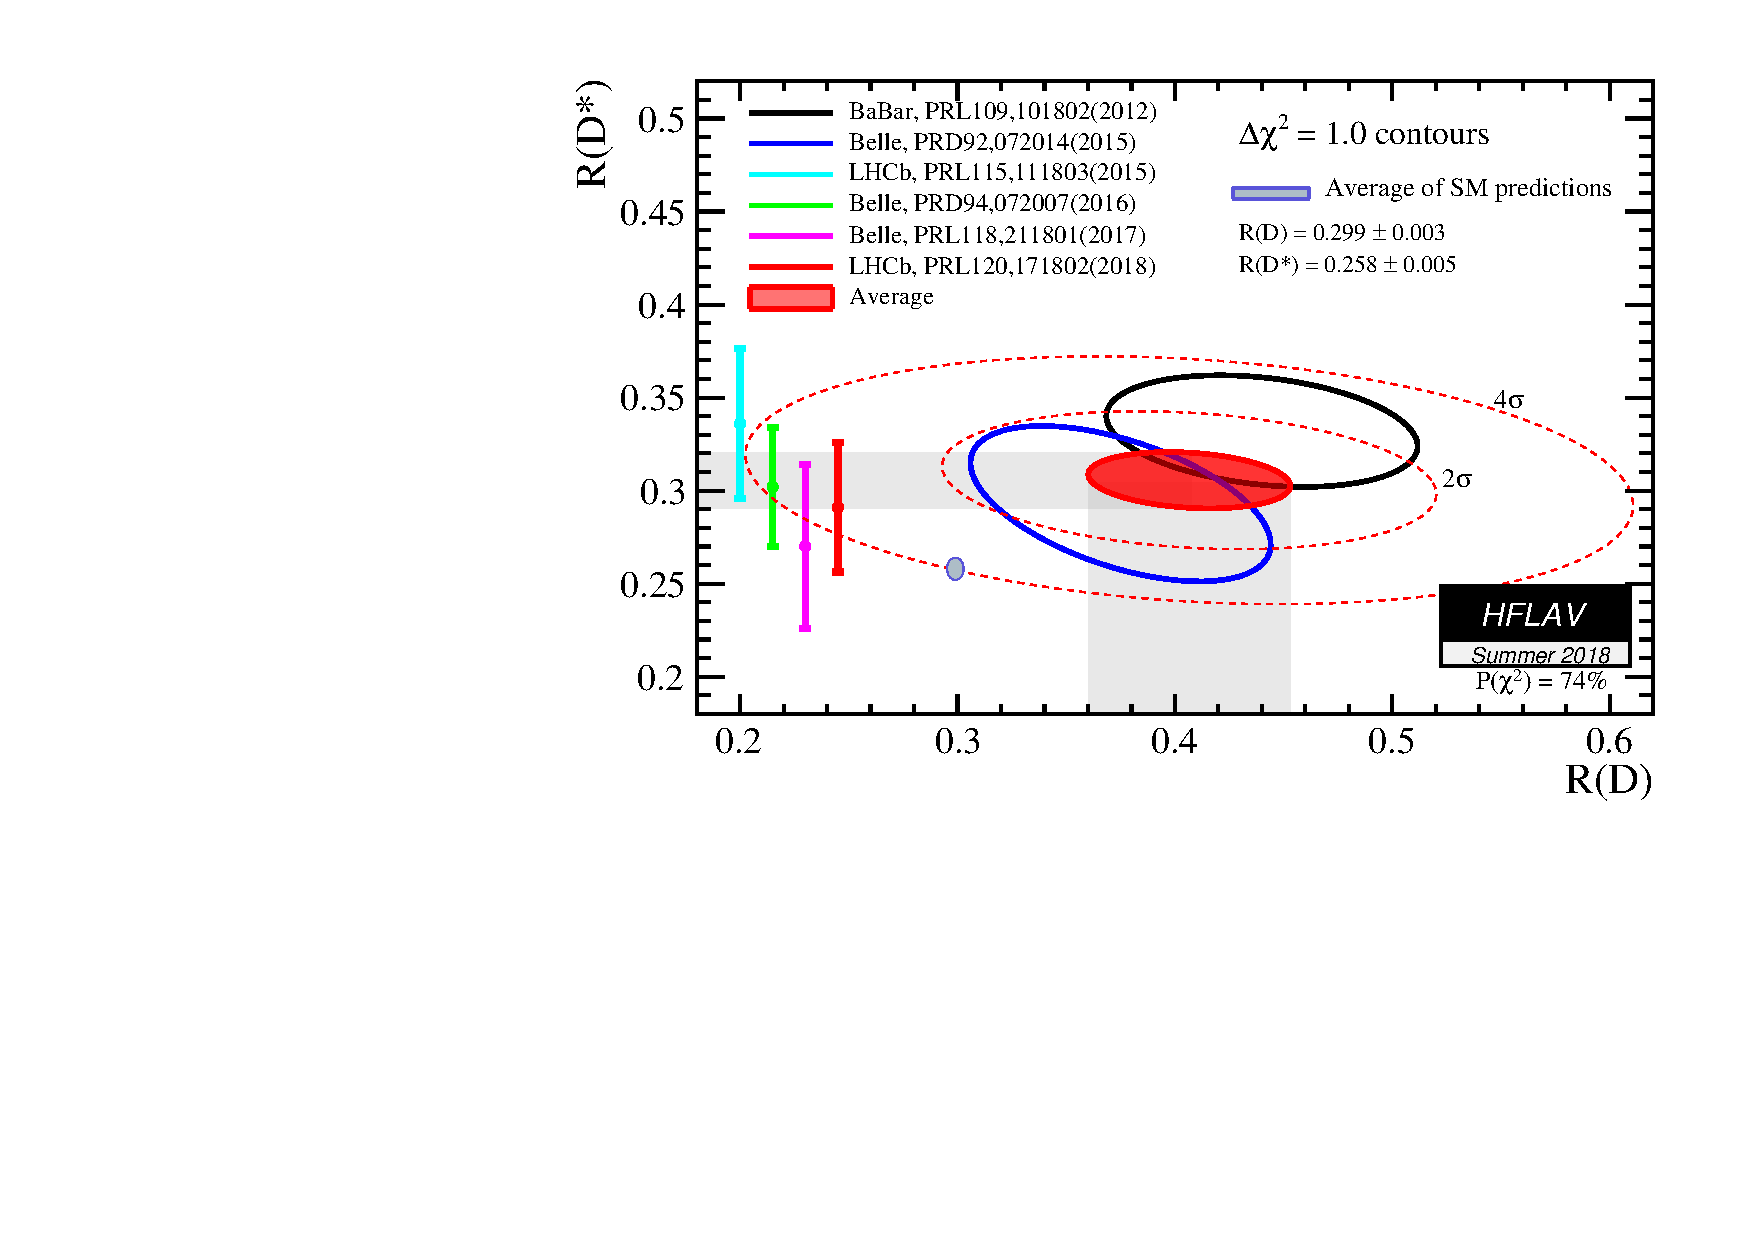
\includegraphics[width=
      0.8\textwidth]{images/rdrds_summer18.pdf}
  \end{center}
  \caption{$R(D^{(*)})$ determinations from SM and measurement
    \cite{HFLAV16}
    \label{fig:ratiotension}}
\end{figure}

There are also tensions in the quantitites \cite{Altmannshofer:2017yso}
\begin{align}
  R_{K^{(*)}} = {\Gamma( B\to K^{(*)}\mu^+\mu^-)\over \Gamma( B\to K^{(*)} e^+e^-)}.
\end{align}
LHCb measured $R_K$ between 1 and 6GeV, and found a disagreement with the SM value \cite{Bobeth:2007dw,Bouchard:2013mia} of 2.6$\sigma$ \cite{Aaij:2014ora}. LHCb also measured $R_{K^*}$ in 2 bins ($0.045<q^2<1.1 $GeV$^2$ and $1.1<q^2<1.6$GeV$^2$), and reported disagreement with the SM prediction \cite{Bordone:2016gaq,Descotes-Genon:2015uva,Capdevila:2016ivx,Capdevila:2017ert,Serra:2016ivr,Straub:2015ica,Altmannshofer:2017fio,Jager:2014rwa} of 2.1-2.3$\sigma$ and 2.4-2.5$\sigma$ respectively \cite{Aaij:2017vbb}.

%% A useful direction we could go in, besides improving the precision of these ratios, is to test other ratios where LFV should show up. For example, in this thesis, we provide a new prediction of $R_{D_s}$, which when combined with future experimental data, will help eludicate this picture.

Each of these anomalies points to one potential new physics scenario: lepton flavour violation (LFV), a breakdown of the lepton flavour universality in the SM discussed in Sec. \ref{sec:fccc}. A consequence of LFV would be that the different leptons generations would no longer have the same coupling to gauge fields. For example, imagine couplings like $U_{ij} \bar{e}_L^i \slashed{W}^+ \nu_L^j$, where $U_{ij}$ is unitary but non-diagonal, then the different lepton generations would have different couplings to $W$. This can lead to a modification of the $B\to D^{(*)}l\nu$ and $B\to K^{(*)}\bar{l}l$ decays rates by different amounts depending on the lepton flavours in the final state, resulting in the ratios $R_{D^{(*)}}$, $R_{K^{(*)}}$ deviating from the SM prediction.

There are broadly speaking two ways one can explain LFV. The first is to posit that there are in fact right-handed neutrinos, $\nu_R$, and neutrinos have Dirac mass terms $m\bar{\nu}_L\nu_R$, from their coupling with the Higgs, just like the charged leptons and quarks. Then, the argument preventing the presence of non-trivial lepton flavour structure in $\mathcal{L}_{\text{FCCC}}$ breaks down, we obtain an equivalent of the CKM matrix for leptons (the Pontecorvo-Maki-Nakagawa-Sakata (PMNS) matrix), and lepton flavour violation is mediated by the $W$. Neutrinos have in fact already been shown to have mass, the PMNS matrix exists, and it's elements have been measured. However, as mentioned already, these effects would be extremely small due to the extreme lightness of the neutrinos. Experiments have looked for evidence of $W$-mediated LFV processes, $\tau\to \mu\gamma$ and $\mu\to e\gamma$, and they found upper bounds for their branching fractions of $4.2\times 10^{-13}$ \cite{Abe:2003sx} and $3.1\times 10^{-7}$ \cite{TheMEG:2016wtm} respectively.

Besides there being no evidence for $W$-mediated LFV, this picture of neutrino masses is not very aesthetically satisfying. It requires unnaturally small Yukawa couplings between the Higgs and the neutrinos. The second, and much more popular approach, to explaining both LFV and neutrino masses, is the presence of new physics.

In the face of evidence against the SM, the most general way to parameterise the space of possible new physics models is to study the Standard Model Effective Theory (SMEFT). In this approach, one introduces a higher dimension, non-renormalisable operators to the standard model (the SM has only renormalisable dimension 4 operators), and impose a hard momentum cutoff $\Lambda$. Then, the SMEFT is
\begin{align}
  \mathcal{L}_{\text{SMEFT}} = \mathcal{L}_{\text{SM}} + \sum_i {c^{(5)}_i\over\Lambda} \mathcal{O}^{(5)}_i + \sum_i {c^{(6)}_i\over\Lambda^2} \mathcal{O}^{(6)}_i + ...
\end{align}
where $\mathcal{O}_i^{(d)}$ is the set of dimension-$d$ operators that satisfy the symmetries of the SM, and $c_i^{(d)}$ are coefficients to be measured, known as Wilson coefficients. Wilson coefficients differing from the SM expectation can be evidence that the SM must be augmented with new fields at energies above $\Lambda$, and the quantum numbers of the associated operators gives information about the quantum numbers of the new fields.

One can fit the avaliable $B\to D^{(*)}l\bar{\nu}$ and $B\to K^{(*)}\bar{l}l$ data to predictions from SMEFT, in order to infer the Wilson coefficients neccesary to explain the anomalies. In \cite{Freytsis:2015qca} it was found that $R_{D^{(*)}}$ can be explained with the $d=6$ operators
\begin{gather}
  \nonumber
  (\bar{c}\gamma_{\mu}P_L b)(\bar{\tau}\gamma^{\mu} P_L \nu_{\tau}), \quad
  (\bar{c}\sigma^{\mu\nu} P_L b)(\bar{\tau} \sigma_{\mu\nu} P_L \nu_{\tau}), \quad
  (\bar{\tau} P_L c^c)(\bar{b}^c P_L \nu_{\tau}), \\
  (\bar{\tau}\gamma_{\mu} P_R b) (\bar{c} \gamma^{\mu} P_L \nu_{\tau}), \quad
  (\bar{\tau}\gamma_{\mu}P_L b)(\bar{c}\gamma^{\mu} P_L \nu_{\tau}), \quad
  (\bar{\tau}P_R c^c)(\bar{b}^c \gamma^{\mu} P_L \nu),
\end{gather}
where $P_{L/R} = (1\pm \gamma_5)/2$, $\psi^c = -i(\bar{\psi}\gamma^0\gamma^2)^T$ and $\bar{\psi}^c = -i(\gamma^0\gamma^2 \psi)^T$. In \cite{Altmannshofer:2017yso}, a similar process found the operators neccesary to explain $R_{K^{(*)}}$:
\begin{gather}
  \nonumber
  (\bar{s}\gamma_{\mu}P_L b)(\bar{e}\gamma^{\mu}e), \quad (\bar{s}\gamma_{\mu}P_L b)(\bar{\mu}\gamma^{\mu}\mu) \\
  (\bar{s}\gamma_{\mu}P_L b)(\bar{e}\gamma^{\mu}\gamma_5e), \quad (\bar{s}\gamma_{\mu}P_L b)(\bar{\mu}\gamma^{\mu}\gamma_5\mu)
\end{gather}
This information, along with constraints from other measurements, strongly reduces the space of possible new physics models that could produce these anomalies. Hot topics include Leptoquarks, $Z'$ models, and partial compositeness \cite{Altmannshofer:2017yso,Freytsis:2015qca,Bauer:2015knc,Crivellin:2015mga}.



%%%%%%%%%%%%%%%%%%

\section{Strong Interaction Physics}
\label{sec:stronginteractions}

The work of this thesis is essentially quantifying the effect the strong interaction has on branching fractions for semileptonic decays. The strong interaction and the observed pattern of hadrons can be explained with Quantum Chromodynamics (QCD). In this section we review the fundamental theory, and the force's physical features.

\subsection{Quantum Chromodynamics}
\label{sec:qcd}

QCD is an $SU(3)$ Yang-Mills gauge theory. The Lagrangian is derived by requiring:
\begin{itemize}
\item
  $N_f$ fermion fields transforming in the fundamental representation of the $SU(3)_C$ gauge group.
\item
  Invariance under that gauge group.
\item
  Renormalizability of all interactions.
\end{itemize}
From these we find \cite{Schwartz:2013pla}
\begin{align}
  \mathscr{L}_{\text{QCD}} &= \sum_i \bar{q}_i (i \slashed{D} - m_i) q_i - {1\over 4} \text{Tr}G_{\mu\nu} G^{\mu\nu} - g{\bar{\theta}\over 64 \pi^2} \epsilon^{\mu\nu\rho\sigma} \text{Tr}G_{\mu\nu} G_{\rho\sigma} \\
  &D_{\mu} = \partial_{\mu} - i g G_{\mu} \,,\quad
  G_{\mu\nu} = [ D_{\mu}, D_{\nu} ].
  \nonumber
\end{align}
$q_i = ( q_{i,r}, q_{i,b}, q_{i,g} )$ are the $N_f$ fermions, vectors in {\it{color space}}, transforming under
\begin{align}
  q_i(x) \to \Lambda(x)q_i(x) \,,\, \bar{q}_i(x) \to \bar{q}_i(x) \Lambda^{\dagger}(x),
  \label{eq:quark_gauge_trans}
\end{align}
where $\Lambda(x)$ is an $SU(3)$ matrix acting on color the color space. $G_{\mu}$ are the $\mathfrak{su}(3)$-valued gluon fields, transforming under the Gauge group like
\begin{align}
  G_{\mu}(x) \to \Lambda(x) G_{\mu}(x) \Lambda^{\dagger}(x) - {i\over g} [ \partial_{\mu} \Lambda(x) ] \Lambda^{\dagger}(x).
  \label{eq:G_gauge_trans}
\end{align}
$g$ is the coupling constant of the theory, often expressed instead as $\alpha_s = (g/4\pi)^2$. $\bar{\theta}$ has strong experimental bounds on it's size, to the extent that for our purposes it can be neglected \cite{ALTAREV1992242}.

The most notable feature of QCD is due to the running of the QCD coupling $\alpha_s$ \cite{PhysRevLett.30.1343}.
\begin{figure}
  \begin{center}
    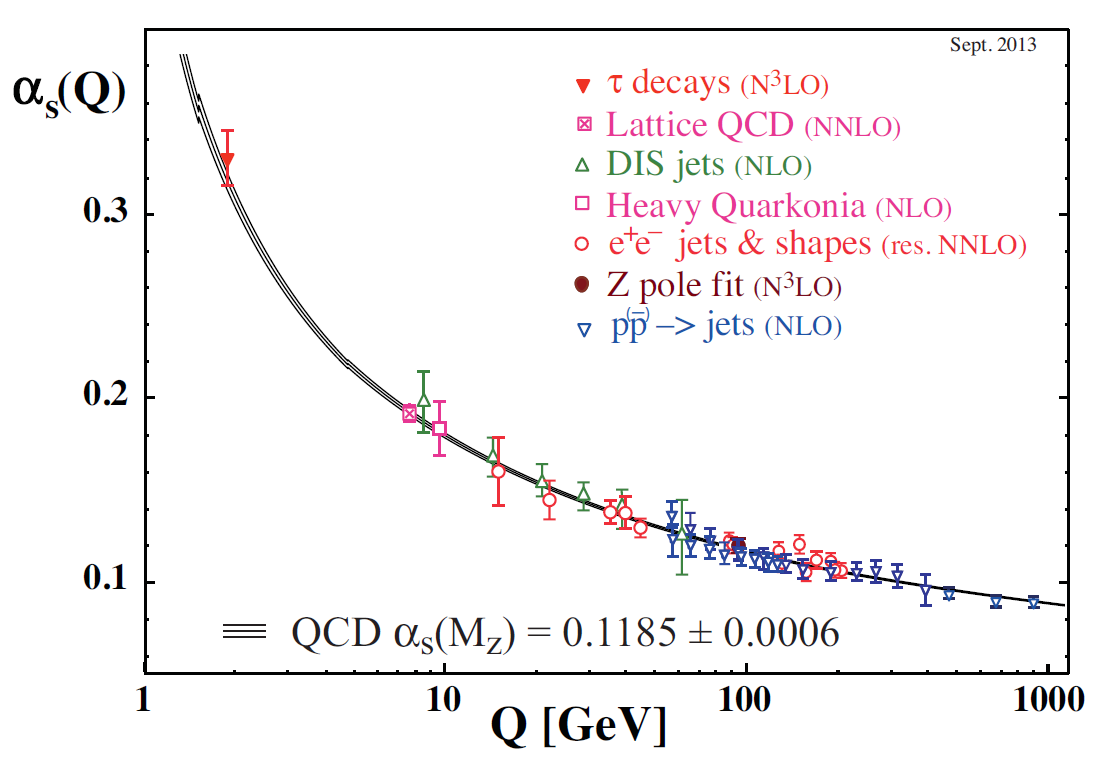
\includegraphics[width=0.7\textwidth]{images/QCD-running-coupling.png}
  \end{center}
  \caption{The relationship between scale $Q$ and the strong coupling constant $\alpha_s$, from the PDG \cite{PhysRevD.98.030001}.}
  \label{fig:semileptonic}
\end{figure}
In contrast with the electroweak force, the coupling of the strong force diverges at low energies. This is referred to as {\it{asymptotic freedom}}. At energies around or below $\Lqcd \sim 0.5$GeV, $\alpha_s$ becomes too large to be a good expansion parameter, and perturbation theory becomes unreliable for making predictions.

At large $\alpha_s$, quarks and gluons become strongly interacting, this is believed to be the source of confinement, the mechanism that bounds quarks together into hadrons. %A common assumption then is that all of the dynamics that occur inside hadrons have energies on the scale of $\Lqcd$.

Broadly speaking there are two approaches to QCD at low energies:
\begin{enumerate}
\item
  Chiral Perturbation theory - an effective theory of hadrons with the same symmetry properties as QCD.
\item
  Lattice simulations - solve the path integral by brute force, eliminating the need for an expansion in $\alpha_s$. This is covered in chapters \ref{chap:latticeqcd} and \ref{chap:latticecalculations}, since it is the method used in the work presented in this thesis.
\end{enumerate}

\subsection{Chiral Symmetry}
\label{sec:chiralsymmetry}

In the limit of $m_i\to 0\,\,\forall i$, QCD develops two new global symmetries between the flavours;
\begin{align}
  \label{eq:vector_chiral}
  q_i &\to \exp(i\theta_a \lambda^{ij}_a) q_j \\
  q_i &\to \exp(i\gamma_5 \theta_a \lambda^{ij}_a) q_j
\end{align}
where $\lambda_a$ are $U(N_f)$ matrices. They are labelled $U(N_f)_V$ and $U(N_f)_A$ respectively, standing for vector and axial-vector.
% Each of these groups can be decomposed into $U(1)_{V/A}\times SU(N_f)_{V/A}$, the $U(1)$ contains the single element corresponding to $\lambda_a=1$, and $SU(N_f)$ contains the elements where $\lambda_a$ are $SU(N_f)$ generators. Neccesary?

Via Noether's theorem, these symmetries imply currents that are conserved in the massless limit \cite{Scherer:2002tk};
\begin{align}
  \label{eq:chiralcurrents}
  V_{\mu}^a = \bar{q} \gamma_{\mu} \lambda_a q \quad,\quad
  A_{\mu}^a = \bar{q} \gamma_{\mu} \gamma_5 \lambda_a q
\end{align}

The way in which the chiral symmetry is realised in quantum mechanics is captured by the {\it{Ward identities}}. There is an infinite number of possible Ward identities, but for the purpose of our work, we only need to consider the most simple of them. %We will derive these below.

Consider the partition function for QCD:
\begin{align}
  \mathcal{Z} = \int [d\psi d\bar{\psi} dA] e^{iS[\psi,\bar{\psi},A]},
\end{align}
where $[d\psi d\bar{\psi} dA]$ represents the functional integral over qark,antiquark and gauge fields. Consider performing a shift of the integration variables of the form \eqref{eq:vector_chiral}, and allow the parameters $\theta_a$ to be local, $\theta_a=\theta_a(x)$. The partition function becomes
\begin{align}
  \mathcal{Z} = \int \mathcal{J} [d\psi d\bar{\psi} dA] ( 1 + i\delta S ) e^{iS[\psi,\bar{\psi},A]}
  \label{eq:partition_transformed}
\end{align}
%$\mathcal{J}$ is the Jacobian of the measure $[d\psi d\bar{\psi} dA]$ under the coordinate transform \eqref{eq:vector_chiral}. In many cases, this will be non-trivial, even if the transform is classically a symmetry of the theory. This can be due to a regularization of the path integral that does not respect the symmetries of the theory. Alternatively, it could be due to an anomaly - an instance of a classical symmetry not holding in quantum mechanics. The symmetries we will be concerned with in this work will always be anomaly-free, so let's set $\mathcal{J}=1$.

$\mathcal{J}$ is the Jacobian of the measure $[d\psi d\bar{\psi} dA]$ under the coordinate transform \eqref{eq:vector_chiral}. In many cases, $\mathcal{J}$ will be non-trivial, due to either regularization schemes that don't respect the symmetry or quantum anomalies. The symmetries we are concerned with here are anomaly free, so $\mathcal{J}=1$.

The effect of the local version of \eqref{eq:vector_chiral} on the action is
\begin{align}
  \delta S = \int d^4x \theta_a(x) \left[ \partial_{\mu} V_a^{\mu}(x) - i\bar{q}(x) [\lambda_a,M] q(x) \right],
\end{align}
where $M = \text{diag}(m_u,m_d,m_s,...)$ acts on flavour. Setting the arbitrary parameters $\theta_a(x)$ to $1$ and removing $\mathcal{Z}$ from each side of \eqref{eq:partition_transformed}, and removing the spacetime integral $\int d^4x$ results in
\begin{align}
  \partial_{\mu}\langle V_a^{\mu} \rangle = i \langle \, \bar{q} [ \lambda_a, M ] q \, \rangle,
  \label{eq:vector_ward}
\end{align}
where $\langle \rangle$ represents a quantum expectation value, the state the expectation value is taken need not be specified since the above derivation does not assume any particular state. Repeating the above steps with the vector chiral transform replaced with the axial-vector chiral transform, one finds
\begin{align}
  \partial_{\mu}\langle A_a^{\mu} \rangle = i \langle\, \bar{q} \{ \lambda_a,M \} q \,\rangle.
  \label{eq:axial_ward}
\end{align}
\eqref{eq:vector_ward} and \eqref{eq:axial_ward} are examples of Ward identities, they describe the non-conservation of the chiral currents.

A useful theorem \cite{Fubini:1964boa} is that partially conserved currents (currents that become conserved when some parameter in the theory vanishes, like $V^{\mu}_a$ and $A^{\mu}_a$) require no renormalisation under any regularisation scheme. %We will now demonstrate this.
The conserved or partially conserved current $J_a^{\mu}$ has a corresponding charge $Q_a(t) = \int d^3x J^{0}(\underline{x},t)$ that is the generator of it's corresponding symmetry transform on Hilbert space. In this case, these charges are members of the Lie algebra of the symmetry group;
\begin{align}
  [ Q_a(t), Q_b(t) ] = if_{abc} Q_c(t),
  \label{eq:charge_commutator}
\end{align}
where $f_{abc}$ are the structure constants of the algebra. Under some regularisation, change in regularisation scheme, or running of scale, each operator in the theory may require multiplicative renormalisations; $Q_a \to Z_Q Q_a$. Equation \eqref{eq:charge_commutator} demands that $Z_Q=1$, so $J^0$ obtains no renormalisation, and if the regularization is lorentz invariant, this carries on to $J^{\mu}$.

%% In the case of the chiral currents $V_a^{\mu},A_a^{\mu}$, the Ward identities \eqref{eq:vector_ward}, \eqref{eq:axial_ward} cause this property to carry onto the operators on the LHS, $\bar{q} [\lambda_a,M] q$ and $\bar{q} \{ \lambda_a,M \} q$, these operators receive no normalisation under any regularisation scheme.

Since one can transform any flavour into any other flavour via the chiral $U(N_f)$ generators, one can build currents charged with any combination of flavours from linear combinations of $V_a^{\mu}$ and $A_a^{\mu}$;
\begin{align}
  \label{eq:vector_ward_indiv}
  V_{ij}^{\mu} &= \bar{q}_i \gamma^{\mu} q_j \,,\quad\quad \partial_{\mu}\langle V^{\mu}_{ij} \rangle = i ( m_i - m_j ) \langle S_{ij} \rangle \\
  A_{ij}^{\mu} &= \bar{q}_i \gamma^{\mu}\gamma^5 q_j \,,\quad \partial_{\mu}\langle A^{\mu}_{ij} \rangle = i ( m_i + m_j ) \langle P_{ij} \rangle
  \label{eq:axial_ward_indiv}
\end{align}
where we have defined $S_{ij} = \bar{q}_iq_j$ and $P_{ij} = \bar{q}_i\gamma^5 q_j$, the scalar and pseudoscalar densities. The non-renormalisation of $V_a^{\mu}$ and $A_a^{\mu}$ carry on to $V_{ij}^{\mu}$ and $A_{ij}^{\mu}$, and onto the operators $( m_i - m_j ) S_{ij}$, $( m_i - m_j ) P_{ij}$ via the Ward identities.

The partially conserved currents $V^{ij}_{\mu}$ and $A^{ij}_{\mu}$ are the same currents that feature in the matrix element of leptonic and semileptonic decays in Sec. \ref{sec:fccc}, and their expectation values appear in amplitudes for leptonic and semileptonic decays. Hence, the fact that these can be related to alternative expectation values via ward identities, and that they obtain no renormalisation, is very useful in the calculation of these amplitudes.

\section{Heavy Quark Physics}

Quarks with mass $m_Q >> \Lqcd$ are referred to as heavy quarks. Charm and bottom quarks are considered heavy: $\Lqcd/m_c \sim 1/4$, $\Lqcd/m_b \sim 1/14$. This separation of scales can come in very useful. They mean one can integrate out the degrees of freedom at $m_Q$, and still have a good description of the dynamics at $\Lqcd$. This philosophy gives rise to Heavy Quark Effective Theory (HQET). We will summarise the aspects of this theory most relevant to our work.

%% The physical picture of a meson containing a heavy quark is very similar to that of a hydrogen atom. In the hydrogen atom, the nucleus has a mass much greater than the characteristic energies of the electron and photons. One can treat the nucleus as a static source of electric charge, and solve to high precision the dynamics of the electron. The electron's behaviour is not affected by the mass or the spin of the nucleus. Similarly, one can consider a heavy quark in a meson to be a static source of colour charge, and solve the $\Lqcd$ dynamics in its presence. The mass and spin of the heavy quark does not effect the light degrees of freedom, this is the well understood {\it{heavy quark symmetries}}. The effective field theories introduced in this section gives us a framework to take this approximation and systematically correct for it.

\subsection{HQET}

HQET is an effective field theory with the cutoff at the heavy quark mass $m_Q$, and terms organized in a series in $\Lambda_{\text{QCD}}/m_Q$. Since at the $b$ (and $c$) mass QCD is perturbative ($\alpha_s(m_Q) << 1$), one can match HQET to perturbative QCD at $m_Q$, then run the couplings of HQET down to produce useful predictions at the confinement scale.

%% It is a useful tool for when we perform extrapolations in heavy quark mass, as it supplies us with explicit expressions for the heavy quark mass dependence on various phenomenological quantities.

\subsubsection{HQET Lagrangian}

We will derive HQET for a single heavy quark interacting with gluons, the generalization to many flavours is straightforward. The fermion part of the Lagrangian is
\begin{align}
  \mathscr{L}_{\text{QCD}} = \bar{Q} ( i\slashed{D} - m_Q ) Q,
  \label{eq:dirac}
\end{align}
where $Q$ is the heavy quark field. Define the heavy quark velocity $v$ according to $v = p_Q/m_Q$. Split $Q$ into ``heavy'' and ``light'' components:
\begin{align}
  \label{eq:hdef}
  Q = h + H\quad : \quad &h = {1\over 2} e^{-im_Q v\cdot x} ( 1 + \slashed{v} ) Q \\
  &H = {1\over 2} e^{-im_Q v\cdot x} ( 1 - \slashed{v} ) Q
\end{align}
with the important property
\begin{align}
  \slashed{v} h = h \quad \slashed{v} H = - H.
\end{align}
In terms of these new fields the Lagrangian becomes
\begin{align}
  \mathscr{L}_{\text{QCD}} = i\bar{h} (v\cdot D) h - \bar{H} ( i(v\cdot D) - 2m_Q ) H
  + i \bar{h} \slashed{D}^{\perp} H + i \bar{H} \slashed{D}^{\perp} h.
  \label{eq:HQET_preintegral}
\end{align}
where $v_{\mu}(v\cdot D)$ is the covariant derivative projected along the direction of $v$, and $D^{\perp} = D - v_{\mu}(v\cdot D)$ are the components perpendicular to $v$. %In the rest frame of the heavy quark, $v = (1,0,0,0)$ so $v_{\mu}(v\cdot D)$ becomes the temporal derivative and $D^{\perp}$ the spacial.
A physical interpretation of the definition of $h$ in \eqref{eq:hdef} can be seen by acting a spacial derivative on the definition of $h$, and by recognising $\partial Q = -i p_Q$, $\partial h = -i p_h$, we find that
\begin{align}
  p_Q = m_Q v + p_h.
\end{align}
Since $p_h << p_Q$, we see that the quark's momentum is dominated by it's mass (the quark is close to on-shell), and the $h$ field represents perturbations around on-shell due to interactions with the lighter degrees of freedom at $\Lambda_{\text{QCD}}$.

From \eqref{eq:HQET_preintegral}, we see that $h$ is a massless field and $H$ has a mass of $2m_Q$. From this Lagrangian we can derive an equation of motion for $H$:
\begin{align}
  ( i(v\cdot D) + 2m_Q) H = i\slashed{D}^{\perp} h,
\end{align}
with the solution
\begin{align}
  H = {1\over i(v\cdot D) + 2m_Q} i\slashed{D}^{\perp} h = {1\over 2m_Q}\sum_{n=0}^{\infty} {(-i(v\cdot D))^n\over 2m_Q} \slashed{D}^{\perp} h.
\end{align}
By substituting this into the Lagrangian we arrive at
\begin{align}
  \mathscr{L}_{\text{HQET}} = i \bar{h} (v\cdot D) h - \bar{h} \slashed{D}^{\perp} {1\over 2m_Q}\sum_{n=0}^{\infty} {(-i(v\cdot D))^n\over 2m_Q} \slashed{D}^{\perp} h.
  \label{eq:HQET_lagrangian}
\end{align}
%This can be found by a more rigorous proof by performing the Gaussian integration over the $H$ field in the path integral {\color{red}{ref!}}.
Since we expect $v\cdot D \sim \Lambda_{\text{QCD}}$, we can interpret the infinite sum as a series in $\Lambda_{QCD}/m_Q$, and truncate it at some order. %For example to $\mathcal{O}(\Lambda_{\text{QCD}}/m_Q)$, we have
%% \begin{align}
%% \mathcal{L}_{\text{HQET}^1} = i \bar{h} (v\cdot D) h - {1\over 2m_Q} \bar{h} \slashed{D}^{\perp 2} h
%% \label{eq:HQET1}
%% \end{align}

Leading order HQET exhibits new symmetries not present in full QCD, known as the heavy quark symmetries. Since $m_Q$ is not present in the leading order Lagrangian, there is a flavour symmetry - a set of $N$ heavy quarks with the same $v$ can be mixed via an $SU(N)$ symmetry. Similarly, due to the absence of spin-mixing matrices, a heavy quark has an $SU(2)$ spin symmetry. This builds up a physical picture of a heavy quark in a meson being a static colour charge, the dynamics at $\Lambda_{\text{QCD}}$ are not effected by its mass or spin.

We will now use HQET to derive a useful theorem used in our work.

%% \subsubsection{Isgur-Wise Function}
%% \label{sec:isgurwise}

%% A consequence of heavy quark symmetry relevant to semileptonic decays are the Wigner-Eckart theorems. Consider a transition amplitude between two heavy pseudoscalar mesons:
%% \begin{align}
%%   \langle M(v) | \bar{h} \Gamma h | M(v') \rangle
%% \end{align}
%% The spin structure of $| M(v) \rangle$ is $\gamma_5 (1-\slashed{v})$, this can be shown with the following argument. The state can be generally written as $| M(v) \rangle = \int d^4x d^4y f(x,y) \bar{h}(x) \gamma_5 q(y) | \Omega \rangle$ where $q$ is the light valence quark and $|\Omega\rangle$ is the interacting vacuum. Using $\slashed{v} h = h$, this can be reexpressed as $| M(v) \rangle = \int d^4x d^4y f(x,y) \bar{h}(x) \gamma_5 (1-\slashed{v}) q(y) | \Omega \rangle /2$. %Then via the spin symmetry, one can always rotate the $h$ spin in the meson state such that it matches the spin of the current, i.e. $h_{\alpha} \bar{h}_{\beta} \to 1_{\alpha\beta} f(h,\bar{h})$.

%% The amplitude can be written as
%% \begin{align}
%% \langle M(v) | \bar{h} \Gamma h | M(v') \rangle = m_M \text{Tr}[ {1\over 2} \gamma_5 (1 - \slashed{v}) \Gamma {1\over 2} \gamma_5 (1 - \slashed{v'}) \mathcal{M}(v,v')]
%% \label{eq:wignereckart1}
%% \end{align}
%% where $\mathcal{M}(v,v')$ can be any gamma-matrix valued function. The $m_M$ factor comes from the relativistic normalisation of the states. A general spin decomposition of this is
%% \begin{align}
%% \mathcal{M}(v,v') = \xi_0(v\cdot v') + \slashed{v} \xi_1(v\cdot v') + \slashed{v'} \xi_2(v\cdot v') + \slashed{v}\slashed{v'} \xi_4(v\cdot v').
%% \end{align}
%% Plugging this into \eqref{eq:wignereckart1}, we can then write the amplitude in terms of a single function:
%% \begin{align}
%% \langle M(v) | \bar{h} \Gamma h | M(v') \rangle = m_M \text{Tr}[ {1\over 2} \gamma_5 (1 - \slashed{v}) \Gamma {1\over 2} \gamma_5 (1 - \slashed{v'}) ] \xi(v\cdot v'),
%% \end{align}
%% where $\xi(v\cdot v') = \xi_0(v\cdot v') + \xi_1(v\cdot v') - \xi_3(v\cdot v') - \xi_4(v\cdot v')$ is known as the Isgur-Wise function. For a general pair of mesons with spin structure $\mathcal{H}$,$\mathcal{H}'$, a transition amplitude between them with a heavy current insertion can always be written as
%% \begin{align}
%% \langle \mathcal{H} | \bar{h} \Gamma h | \mathcal{H}' \rangle = \xi(v\cdot v') Tr[ \bar{\mathcal{H}} \Gamma \mathcal{H} ] + \order{\Lambda_{\text{QCD}}\over m_Q}
%% \end{align}
%% So all heavy semileptonic decays involving any combination of masses or spins are described by a single non-perturbative function, $\xi(v\cdot v')$. Examples relevant to the work of this thesis are:
%% \begin{align}
%% \langle D(v') | \bar{c_{v'}} \gamma^{\mu} b_v | B(v) \rangle &= \sqrt{m_B m_D} ( v + v')^{\mu} \xi(v\cdot v') \\
%% \langle D^*(v') | \bar{c_{v'}} \gamma^{\mu} b_v | B(v) \rangle &= i \sqrt{m_B m_D*} \epsilon^{\mu\nu\alpha\beta} \varepsilon_{\nu}^* v'_{\alpha} v_{\beta} \xi(v\cdot v')  \\
%% \langle D^*(v') | \bar{c_{v'}} \gamma^{\mu}\gamma_5 b_v | B(v) \rangle &= \sqrt{m_B m_D*} [ \varepsilon^{*\mu}(v\cdot v' + 1) - v^{'\mu} \varepsilon^*\cdot v] \xi(v\cdot v').
%% \end{align}
%% Here we have subscripted the fields $c_{v'}$,$b_v$ to specify the velocity used to separate those fields from the heavy components e.g. in eq. \eqref{eq:hdef}.

\subsubsection{Luke's Theorem}
\label{sec:Luke}

Luke's theorem, which can be derived from the Ademollo-Gatto (AG) theorem, tells us the leading order heavy quark mass dependence of form factors. First we will derive the AG theorem. We will follow the proof given in \cite{Lebed:1991sq}.

Consider the transition amplitude
\begin{align}
  \langle \alpha | Q_a | \beta \rangle,
\end{align}
where $Q_a$ is a conserved charge associated with some global symmetry $\mathcal{G}$, and $|\alpha\rangle$ and $|\beta\rangle$ belong to an irrep of $\mathcal{G}$. Imagine explicitly breaking the symmetry with a term like $\mathscr{L}_{\text{break}} = \lambda \mathcal{O}_{\text{break}}$. The states in the broken theory can be expressed as
\begin{align}
  |\beta \rangle = c_{\beta\beta} | \beta' \rangle + \sum_{m} c_{\beta m} | m' \rangle \\
  \langle \alpha | = c^*_{\alpha\alpha} \langle \alpha' | + \sum_{n} c^*_{\alpha n} \langle n' |.
\end{align}
where primed states are the new basis of states belonging to irreps of $\mathcal{G}$, after the breaking. Here $|m'\rangle$ can only be states that can be mixed with $| \beta \rangle$ by $\mathcal{O}_{\text{break}}$, i.e., via the broken dynamics of the theory. Similarly for $\langle n' |$ and $\langle \alpha |$. The transition amplitude becomes
\begin{align}
  \nonumber
  \langle \alpha | Q_a | \beta \rangle
  &= c_{\alpha\alpha}^* c_{\beta\beta} \langle \alpha' | Q_a | \beta' \rangle \\
  \nonumber
  &+ \sum_m c_{\alpha\alpha}^* c_{\beta m} \langle \alpha' | Q_a | m' \rangle \\
  \nonumber
  &+ \sum_n c_{\alpha n}^* c_{\beta \beta} \langle n' | Q_a | \beta \rangle \\
  &+ \sum_m\sum_n c_{\alpha n}^* c_{\beta m} \langle n' | Q_a | m' \rangle.
  \label{eq:AGproofexpanded}
\end{align}
The theorem applies to the situation where $|n'\rangle$ and $|m'\rangle$ live in different $\mathcal{G}$ irreps to $|\alpha\rangle$ and $|\beta \rangle$ (we assume $|\alpha\rangle$ and $|\beta \rangle$ to be in the same irrep otherwise the transition amplitude would vanish). In this case the amplitudes in the second and third terms vanish. Now consider the order of the coefficients $c_{nm}$. We can assume that $c_{nm} = \order{\lambda}$ for arbitrary $n,m \neq \alpha,\beta$, since switching off the symmetry breaking by setting $\lambda=0$ should cause $|\alpha\rangle $ and $|\alpha'\rangle$ to coencide. Then, using the normalization of the states $\sum_{n} |c_{\alpha n} |^2 = 1$, we find $c_{\alpha\alpha} = \sqrt{1 - \order{\lambda}^2} = 1 + \order{\lambda^2}$, and similarly for $c_{\beta\beta}$. Applying this to the two surviving terms in \eqref{eq:AGproofexpanded}, we end up with
\begin{align}
  \langle \alpha | Q_a | \beta \rangle = 1 + \order{\lambda^2}
\end{align}
This is the AG theorem: if the current $Q_a$ and the symmetry breaking term $\mathcal{O}_{\text{break}}$ act orthogonally on the states, the transition amplitude can have at most a second order correction in the symmetry breaking parameter.

Now we will apply this to HQET to produce Luke's theorem. Consider a transition including two heavy quarks ($b$ and $c$). Then, the heavy quark symmetry is a spin symmetry for each flavour and a flavour symmetry between them. The leading order spin symmetry breaking terms can be found from \eqref{eq:HQET_lagrangian} to be
\begin{align}
  {1\over 4m_Q} \bar{h} \gamma^{\mu} \gamma^{\nu} F_{\mu\nu} h.
\end{align}
for both $h=b$ and $h=c$. The leading order flavour breaking term is
\begin{align}
  \left({1\over 2m_b} - {1\over 2m_c} \right) {1\over 2} \bar{h} \sigma_z \slashed{D}^{\perp 2} h,
\end{align}
where now $h = (b,c)$ and the $\sigma_z$ is the third pauli matrix acting on flavour. These terms cause states, for example $| B \rangle$ to mix with states $|n'\rangle$, each being of the order of at least one of the following: $1/2m_b$,$1/2m_c$, and $(1/2m_b - 1/2m_c)$. It can be shown \cite{Lebed:1991sq} that the leading order symmetry breaking terms can only mix pseudoscalar and vector mesons with other irreps of the heavy quark symmetries. Hence, for example, in the $B \to D^*$ transition we can write
\begin{align}
  \langle D | \bar{c}\gamma_{\mu} b | B \rangle &= \xi + \order{\left( {1\over 2m_b} - {1\over 2m_c} \right)^2}, \\
  \langle D | \bar{c}\gamma_{\mu}\gamma_5 b | B \rangle &= \xi + \order{\left( {1\over 2m_b} - {1\over 2m_c} \right)^2}.
\end{align}
where $\xi$ is some $b$- and $c$-mass independent number.

This carries onto the pseudoscalar-vector and pseudoscalar-pseudoscalar form factors at zero recoil
\begin{align}
  \label{eq:hA1}
  h_{A_1}(1) &= \eta_A \left( 1 + {l_V\over (2m_c)^2} + {l_A\over m_b m_c} - {l_P\over (2m_b)^2} \right), \\
  h_+(1) &= \eta_V \left( 1 - l_P \left( {1\over (2m_b)^2} - {1\over (2m_c)^2} \right) \right),
  \label{eq:hplus}
\end{align}
where here $h_+$ comes from an HQET-inspired parameterisation of pseudoscalar-pseudoscalar transition amplitudes alternative to \eqref{eq:formfactors_experimental}:
\begin{align}
  {\langle M' | V^{q_1q^2}_{\mu} | M \rangle \over \sqrt{Mm}} = h_+(w)(v+v')_{\mu} + h_-(w)(v-v')_{\mu}.
  \label{eq:pseudoscalar_hqet}
\end{align}
The factors $\eta_{A,V}$ in \eqref{eq:hA1} and \eqref{eq:hplus} are matching factors between QCD and HQET, and can contain logarithms of heavy masses. The factors $l_{V,A,P}$ are free non-perturbative parameters that must be fixed by some non-perturbative calculation e.g. a lattice QCD calculation.

%% As we move away from the infinite-mass limit, $\xi$ becomes $h_+$, and $h_-$ becomes non-zero. In this case we see that
%% \begin{align}
%% h_+(q^2_{\text{max}}) &= ( 1 + \order{ \epsilon_b^2}
%% + \order{\epsilon_c^2} \\ &+ \order{\left( \epsilon_b - \epsilon_c \right)^2} ) \\
%% h_-(q^2_{\text{max}}) &= ( \order{ \epsilon_b }
%% + \order{ \epsilon_c } + \order{ \epsilon_b - \epsilon_c } )
%% \end{align}
%% Away from $q^2_{\text{max}}$, the velocities for the $b$ and $c$ quarks become different, resulting in a new flavour breaking term in the effective Lagrangian;
%% \begin{align}
%% i \bar{c} (v - v')\cdot D c \sim \order{1-{E_D\over M_D}} + \order{ \textbf{p}_D\over M_D }
%% \end{align}
%% where to deduce the orders we took the rest frame of the $B$ meson. This results in extra corrections of these orders (raised to the second power) in the form factors.

%% \subsubsection{Second Order Form Factors}

%% The process in \ref{sec:isgurwise} of decomposing matrix elements into general expressions parameterized by non-perturbative functions can be extended beyond leading order in HQET. In \cite{Falk:1992wt} this process was continued to second order in $1/m_b$ and $1/m_c$ for $B\to D^{(*)}$ transitions. The form factors for general $v,v'$ that are relevant to our work, were found to have the forms
%% \begin{align}
%% h_+ &= \xi + (\epsilon_b + \epsilon_c ) L_1 + ( \epsilon_b^2 + \epsilon_c^2 ) l_1 + \epsilon_b \epsilon_c \phi_1 \\
%% h_- &= ( \epsilon_c - \epsilon_b )L_4 + (\epsilon_c^2-\epsilon_b^2) l_4\\
%% h_{A_1} &= \xi + \epsilon_c  L_{25} + \epsilon_b L_{14} + \epsilon_c^2 l_{25} + \epsilon_b^2 l_{14} + \epsilon_c\epsilon_b \phi_2
%% \end{align}
%% where, due to the normalization of the form factors for $m_c=m_b$ at $q^2_{\text{max}}$;
%% \begin{align}
%% L_1(q^2_{\text{max}}) = L_{25}(q^2_{\text{max}}) = L_{14}(q^2_{\text{max}}) = 0
%% \end{align}
%% A calculation using the non-relativistic constituent quark model \cite{PhysRevD.39.799} estimates the factor $l_1(q^2_{\text{max}}) = -3m_q^2$ where $q$ is the spectator of the decay.

\subsection{NRQCD}

An effective field theory closely related to HQET is Non-Relativistic QCD (NRQCD). This differs from HQET only by the power counting; instead of organizing terms in the Lagrangian according to their order in $\Lambda_{\text{QCD}}/m$, the terms are organized in terms of powers of the heavy quark's spacial velocity $v \sim |{\textbf{p}}|/m$. NRQCD is derived with the following process:
\begin{itemize}
\item
  Separate the quark and antiquark components of the heavy quark. Since a non-relativistic fermion is decoupled from its antiparticle, our action only requires to describe the top two components of a Dirac spinor.
  Define the antiquark-free 2-component spinor $h$ via the Foldy-Wouthuysen transformation $\psi \to h = e^{ {\bf{\gamma}}\cdot {\bf{D}}/2m} \psi$ \cite{PhysRev.78.29}. This acts to remove the ${\bf{\gamma}}\cdot {\bf{D}}$ term from the Dirac part of the Lagrangian, which is the only part that couples the fermion to the anti-fermion.
\item
  Define power-counting by considering the expected expectation values of operators for heavy mesons \cite{Lepage:1992tx}. The three relevant scales concerning the heavy meson are $M$,$p\sim Mv$ and $E_K\sim Mv^2$, where $M$ is the meson mass, $p$ the spacial momentum and $E_K$ the kinetic energy. By relating operators to these three scales, we deduce their order in $v$. Start with the normalization of a scalar current:
  \begin{align}
    \langle M | \int d^3x h^{\dagger}(x) h(x) | M \rangle \sim 1,
    \label{eq:nrqcd_scalarnormalization}
  \end{align}
  where $| M \rangle$ is some heavy meson state. Since we expect the meson state to be localized in a region of size $1/p$, we can assert that
  \begin{align}
    \int d^3x \sim {1\over p^3}.
  \end{align}
  From this and \eqref{eq:nrqcd_scalarnormalization}, we find $h \sim p^{3/2} \sim v^{3/2}$.
  The order of the derivative operator can be deduced from
  \begin{align}
    E_K = \langle M | \int d^3x h^{\dagger}(x) {\underline{D}^2\over 2M} h(x) | M \rangle
  \end{align}
  to be $D \sim v$. Following such a chain of arguments, we can deduce the order in $v$ of any operator.

\item
  The Lagrangian to $\order{v^n}$ is then simply all of the operators satisfying the symmetries of QCD of orders below $v^n$, with some Wilson coefficients \cite{Lepage:1992tx}. To $\order{v^6}$:
  \begin{align}
    \nonumber
    &\mathscr{L}_{\text{NRQCD}} = h^{\dagger} \Bigg( i D_0 + {{\textbf{D}}^2 \over 2m} + c_1 {{\textbf{D}}^4\over m^3}
    + c_2 g{{\textbf{D}}\cdot {\textbf{E}} - {\textbf{E}} \cdot {\textbf{D}} \over m^2} \\
    \nonumber
    &+ c_3 ig{ {\bf{\sigma}}\cdot ({\textbf{D}}\times {\textbf{E}} - {\textbf{E}}\times {\textbf{D}})\over m^2}
    + c_4 g{ {\bf{\sigma}}\cdot {\textbf{B}}\over m} \\
    + \nonumber
    & f_1 g{\{{\textbf{D}}^2,{\bf{\sigma}}\cdot {\textbf{B}}\}\over m^3 }
    + f_2 ig{\{ {\textbf{D}}^2,{\bf{\sigma}}\cdot ( {\textbf{D}}\times {\textbf{E}} - {\textbf{E}}\times {\textbf{D}})\}\over m^4 }
    + f_3 ig^2 {{\bf{\sigma}}\cdot {\textbf{E}}\times {\textbf{E}}\over m^3}  \Bigg)h \\
    \nonumber
    &+ d_1 { (h^{\dagger} H) (H^{\dagger} h) \over m^2} + d_2 { (h^{\dagger} {\bf{\sigma}} H) \cdot  (H^{\dagger}{\bf{\sigma}} h) \over m^2} \\
    &+ d_3 \sum_a {(h^{\dagger} T^a H) (H^{\dagger} T^a h) \over m^2} + d_4 \sum_a {(h^{\dagger} T^a {\bf{\sigma}} H) \cdot (H^{\dagger} T^a {\bf{\sigma}} h) \over m^2}
  \end{align}
  ${\textbf{E}}$ and ${\textbf{B}}$ are the chromoelectric and chromomagnetic fields, $T^a$ are fundemental representation of the $SU(3)$ color generators, and $H$ is the antiquark components of the heavy quark. $c_{1,2,3,4},f_{1,2,3},d_{1,2,3,4}$ are Wilson coefficients, that can be fixed by perturbative matching to full QCD at the cutoff (the heavy quark mass, where QCD is perturbative).

\end{itemize}
 % background and motivation
\chapter{Lattice Quantum Chromodynamics}
\label{chap:latticeqcd}

As mentioned in Sec. \ref{sec:qcd}, at low energies QCD becomes non-perturbative. In other words, the coupling $\alpha_s$ becomes $\mathcal{O}(1)$, and an expansion in $\alpha_s$ (as in perturbation theory) will not be dominated by the leading orders. In order to calculate observables of low energy QCD (like hadronic form factors), we require an alternative to perturbation theory.

The expectation value of an observable $\mathcal{O}$ in QCD can be expressed as a path integral:
\begin{align}
  \langle \mathcal{O} \rangle = {1\over Z}\int [dG d\psi d\bar{\psi}] \, \mathcal{O} \, e^{iS[G,\psi,\bar{\psi}]},
\end{align}
where $G$ is the gauge field, $\psi$($\bar{\psi}$) are the (anti)fermion fields, $S$ is the classical action, and $[dG d\psi d\bar{\psi}]$ denotes integration over all configurations of the gauge and fermion fields. $Z$ is the partition function. In the perturbative approach, we would expand $\exp(-\text{interacting part of }S )$ resulting in a power series in the gauge coupling populated by Feynman diagrams.

We must instead carry out the integral directly, by numerical brute force. Since it is not numerically feasible to carry out an infinite number of integrals, one must approximate spacetime as a discrete 4-dimensional lattice with spacing $a$ between lattice sites, finite spacial volume $L_x^3=(aN_x)^3$ and finite temporal extent $L_t=aN_t$ ($N_{x,t}\in \mathbb{N}$). The functional integral can be replaced with
\begin{align}
  \int [dG d\psi d\bar{\psi}] = \prod_{n} \int dU(x_n) d\psi(x_n) d\bar{\psi}(x_n),
\end{align}
where $n$ is a 4-vector with integer components labelling the sites, and $x_n^{\mu} = an^{\mu}$.
This has a second benefit which is to naturally regularize the theory with a momentum cutoff $\Lambda \sim \pi/a$. The gauge field has been replaced with the {\it{gauge link}} $U$, to be defined in the following section.

Typically one uses lattices that have periodic boundary conditions in the temporal direction, i.e $\psi(x+aN_t \hat{t}) = \psi(x)$. This reduces unwanted effects in expectation values of operators due to the finite temporal extend. In all the work in this thesis we use periodic temporal boundary conditions.

To avoid having to integrate over imaginary numbers (equivalently to avoid the scourge of the {\it{sign problem}} \cite{deForcrand:2010ys}), one also performs a {\it{Wick rotation}}. This is the redefinition $t\to it$, which changes the metric from Minkowski to Euclidean, and changes the weight $\exp(iS) \to \exp(-S)$. This has the advantage that it turns the quantum path integral into simply an average in statistical mechanics, this means we can apply all of the machinery of statistical mechanics to computing expectation values.

To obtain the 'real world' result for some expectation value, where real world means $a=0$, one must perform the path integral at a number of different $a$ values, and then extrapolate the results to $a=0$.

One must choose a discretized version of the QCD action, one that becomes continuum QCD in the $a\to 0$ limit. This is a far from trivial step. There is an infinite number of choices of lattice actions that become QCD in the continuum limit. There therefore is a huge literature of different choices of discrete lattice actions. Different collaborations use different actions, and there is never-ending argument about the merits and pitfalls of each.

The rest of this chapter is dedicated to motivating and detailing the choices of discretisation used in the work of this thesis.

\section{Lattice Gauge Fields}
\label{sec:gaugefields}

%Often the best way to introduce some sophisticated method or technique is to first show how the naive approach breaks down.
Imagine attempting a naive discretisation of the QCD action. Derivatives can be replaced with something like
\begin{align}
  \partial_{\mu}f(x) \to {1\over 2a} \left( f(x+a\hat{\mu}) - f(x-a\hat{\mu}) \right)
\end{align}
where $\hat{\mu}$ is the unit vector in the $\mu$ direction. The quark kinetic part of the QCD action, $\bar{q}\slashed{D}q$, becomes
\begin{align}
  {1\over 2a} \bar{q}(x)\gamma^{\mu}q(x+a\hat{\mu}) - {1\over 2a} \bar{q}(x)\gamma^{\mu}q(x-a\hat{\mu}) - ig\bar{q}(x)G_{\mu}(x)\gamma^{\mu} q(x).
\end{align}
This is no longer invariant under gauge trasforms \eqref{eq:quark_gauge_trans}, for example the first term becomes $\bar{q}(x)\Lambda(x)^{\dagger} \Lambda(x+a\hat{\mu}) q(x+a\hat{\mu})$. The finite distance between lattice sites force us to think more carefully about the interpretation of gauge symmetry on a lattice.

Formally speaking, a gauge field is a connection on a fibre bundle. I'll unpack what this means. At each point $x$, there is a space of possible color vectors that a quark field $q(x)$ could be, call it $V_x$. $V_x$ is a {\it{fibre}}. Spacetime is called the {\it{base space}} in this context, there is a fibre at each point in the base space.

The problem with our non-gauge-invariant terms above is that we are trying to compare color vectors in different fibres. To compare color vectors at two different fibres, one must {\it{parallel transport}} the vector from one point to another, according to some rule of how it should change. This rule is called the {\it{connection}}. In our case the parallel transport is a Wilson line:
\begin{align}
  \nonumber  &W(x,y) : V_y \to V_x, \\ &W(x,y) = Pe^{ig\int dc\,\cdot\, G }.
\end{align}
where $c$ is some curve between $x$ and $y$, and $P$ orders the operation of the gauge field $G$ on the fibres, i.e. it operates at $x$ first and $y$ last. A wilson line transforms under the gauge group like $W(x,y)\to \Lambda(x)W(x,y)\Lambda^{\dagger}(y)$, so operators like $\bar{q}(x)W(x,y)q(y)$ are gauge-invariant, reflecting the fact that the color vector $q(y)$ has been parallel transported into the same fibre as $\bar{q}(x)$.

\begin{figure}[htb!]
  \begin{center}
    \vspace{-10pt}
    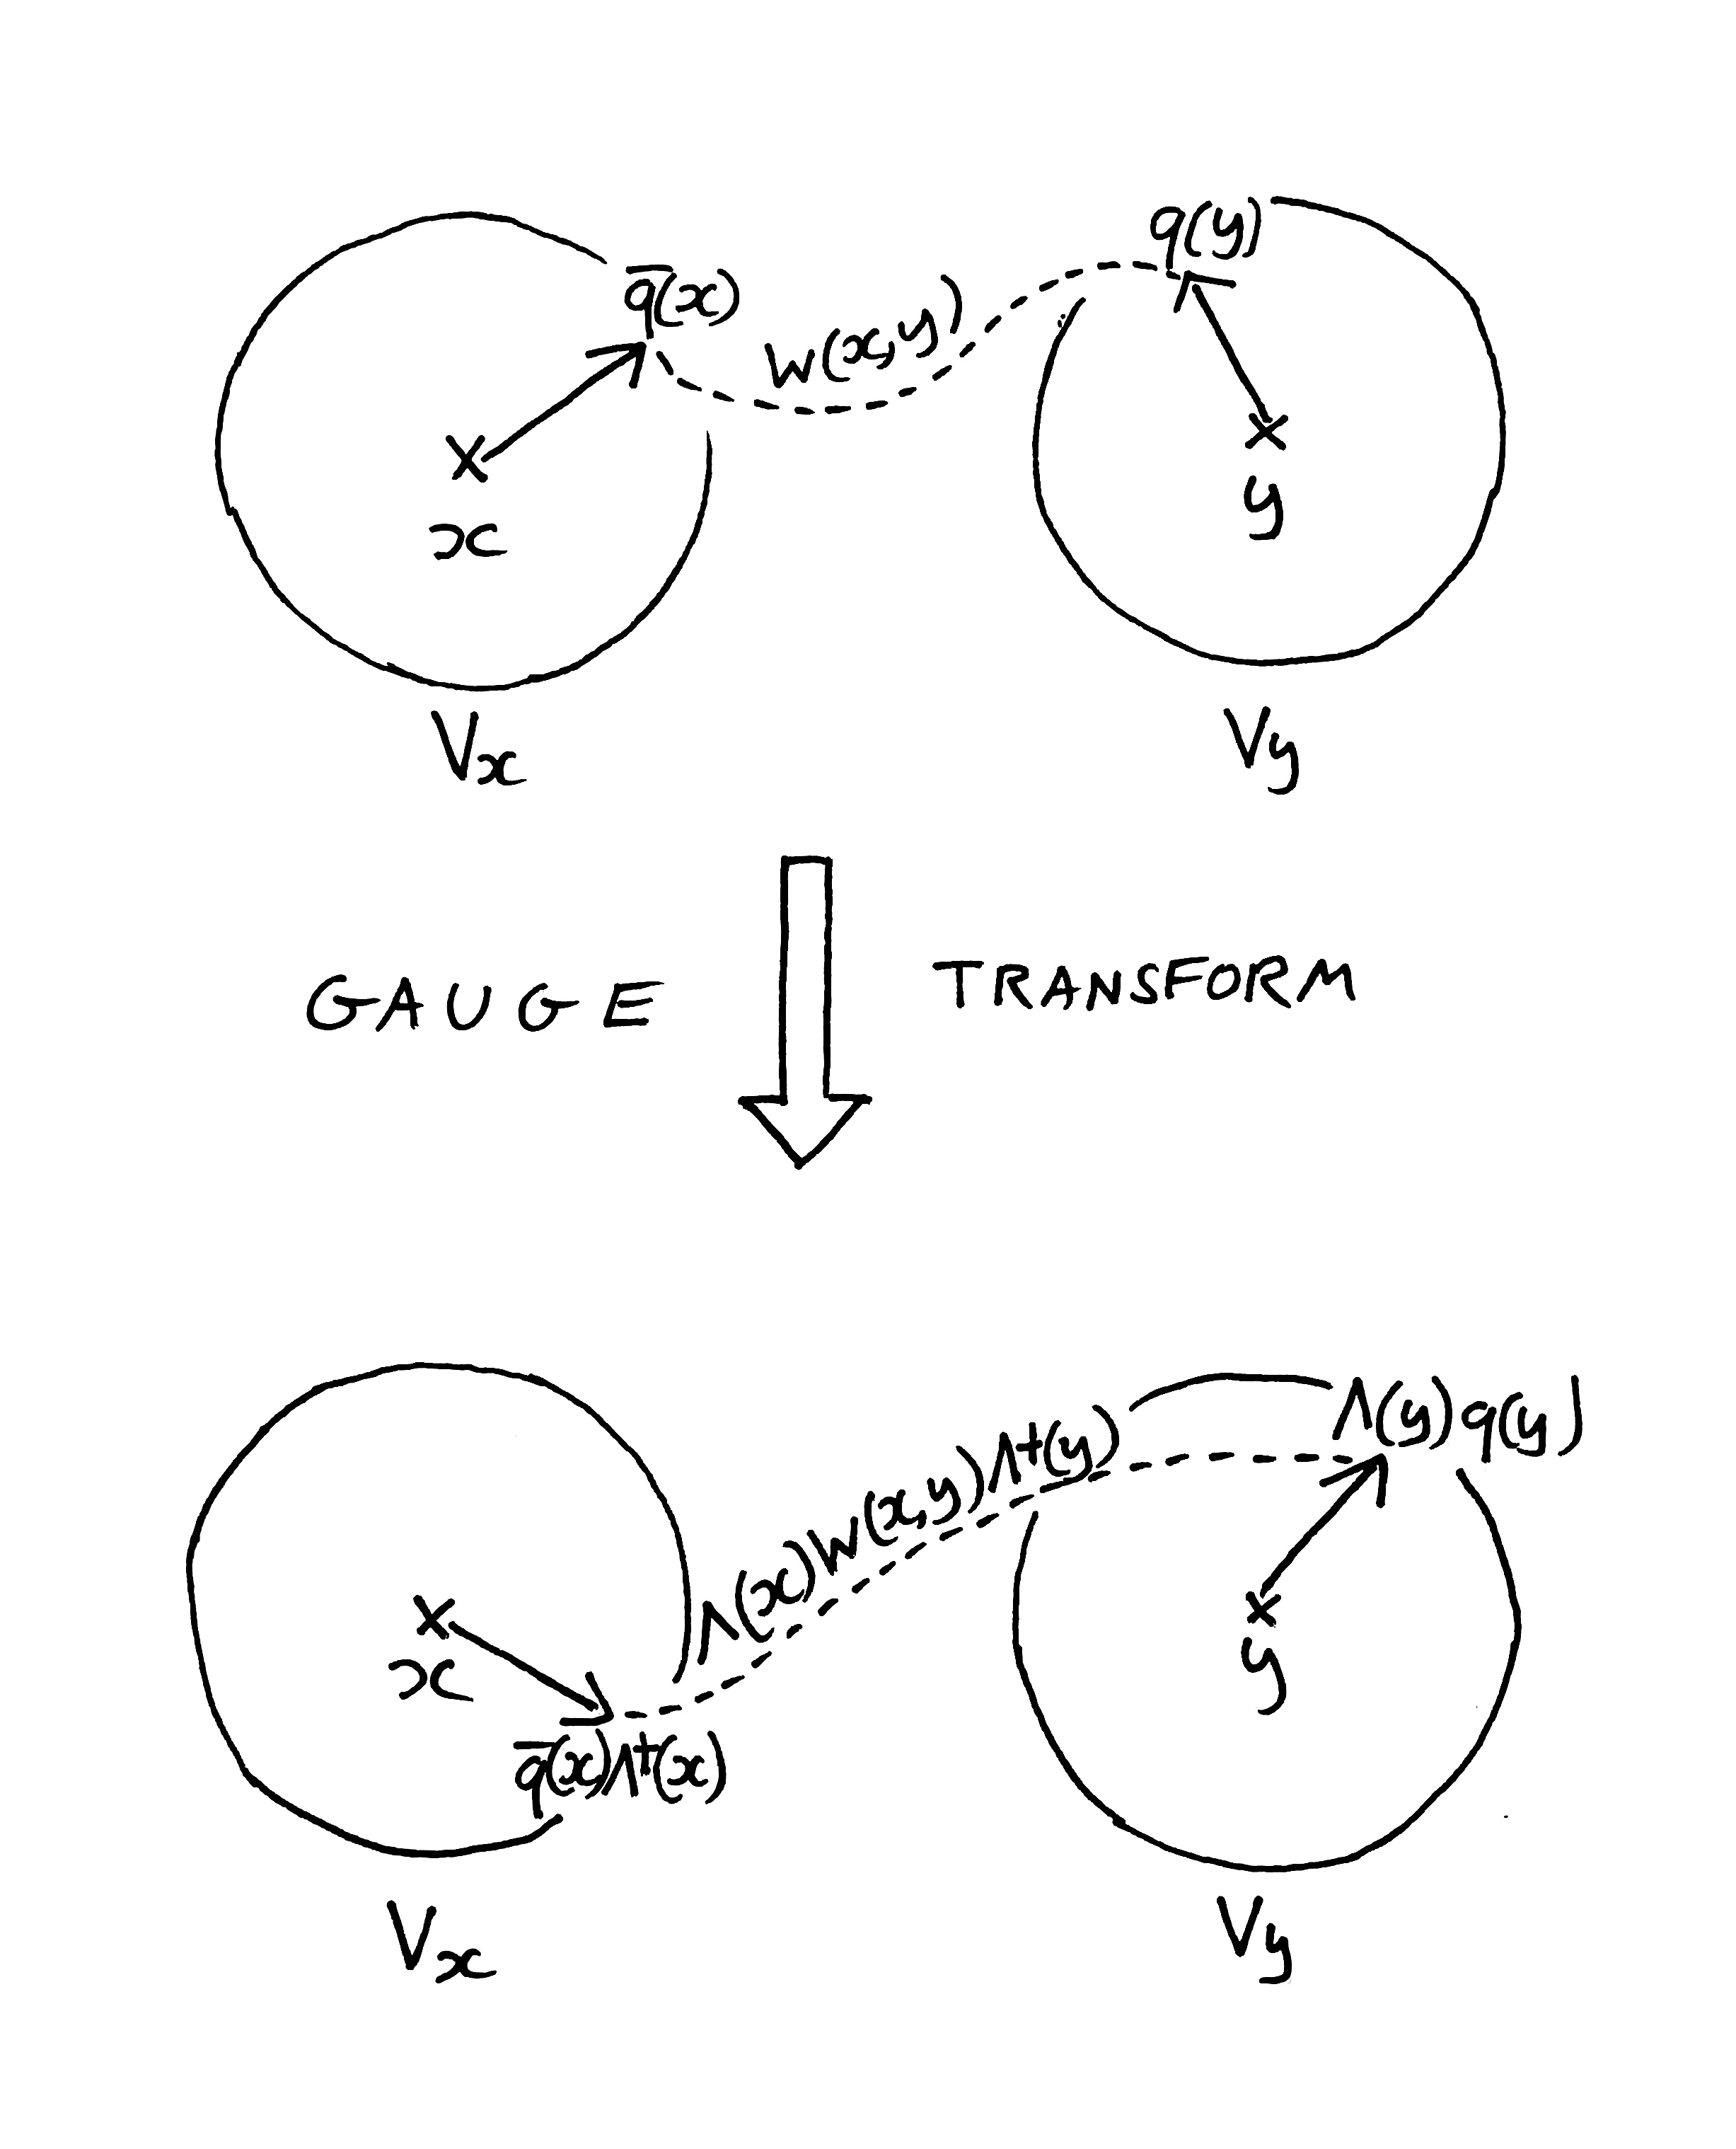
\includegraphics[width=0.55\textwidth]{images/fibres.jpg}
    \caption{Depiction of color spaces (fibres) at two points in spactime (base space) with the value of the quark field $q$ represented at each point as a color vector, and the connection $W(x,y)$ needed to compare the two color vectors. A gauge transform changes the two vectors in different ways, for the comparison to be gauge independent, the connection must also transform appropriately.}
  \end{center}
  \vspace{-10pt}
\end{figure}

On a lattice the natural degrees of freedom are no longer the elements of the Lie algebra, $G_{\mu}$, but Wilson lines connecting adjacent lattice sites, also known as {\it{links}}:
\begin{align}
  U_{\mu}(x) \in SU(3)\,\,: V_x \to V_{x+a\hat{\mu}}\,,
\end{align}
that Gauge transform like
\begin{align}
  U_{\mu}(x) \to \Lambda(x) U_{\mu}(x) \Lambda^{\dagger}(x+a\hat{\mu}).
\end{align}
Then, a bilinear of color vectors at any two points can be made to be gauge invariant by including a path between them made of links. For example;
\begin{align}
  \nonumber
  \bar{q}(x)U_{\mu}(x)q(x+a\hat{\mu}) \quad \to\quad &[\bar{q}(x)\Lambda^{\dagger}(x)](\Lambda(x) U_{\mu}(x) \Lambda^{\dagger}(x+a\hat{\mu})) [\Lambda(x+a\hat{\mu})q(x+a\hat{\mu})]
  \\
  &= \bar{q}(x)U_{\mu}(x)q(x+a\hat{\mu}).
  %% \bar{q}(x)U_{\mu}(x)U_{\nu}(x+a\hat{\mu})q(x+a\hat{\mu}+a\hat{\nu}) \to&
  %% \bar{q}(x)\Lambda^{\dagger}(x) \\ \nonumber
  %% &(\Lambda(x) U_{\mu}(x) \Lambda^{\dagger}(x+a\hat{\mu})) \\ \nonumber
  %% &(\Lambda(x+a\hat{\mu}) U_{\mu}(x+a\hat{\mu}) \Lambda^{\dagger}(x+a\hat{\mu}+a\hat{\nu})) \\ \nonumber
  %% &\Lambda(x+a\hat{\mu}+a\hat{\nu}) q(x+a\hat{\mu}) \\ \nonumber
  %% &= \bar{q}(x)U_{\mu}(x)U_{\nu}(x+a\hat{\mu})q(x+a\hat{\mu}+a\hat{\nu}).
\end{align}

\begin{figure}[htb!]
  \begin{center}
    \hspace{+20pt}
    \vspace{-10pt}
    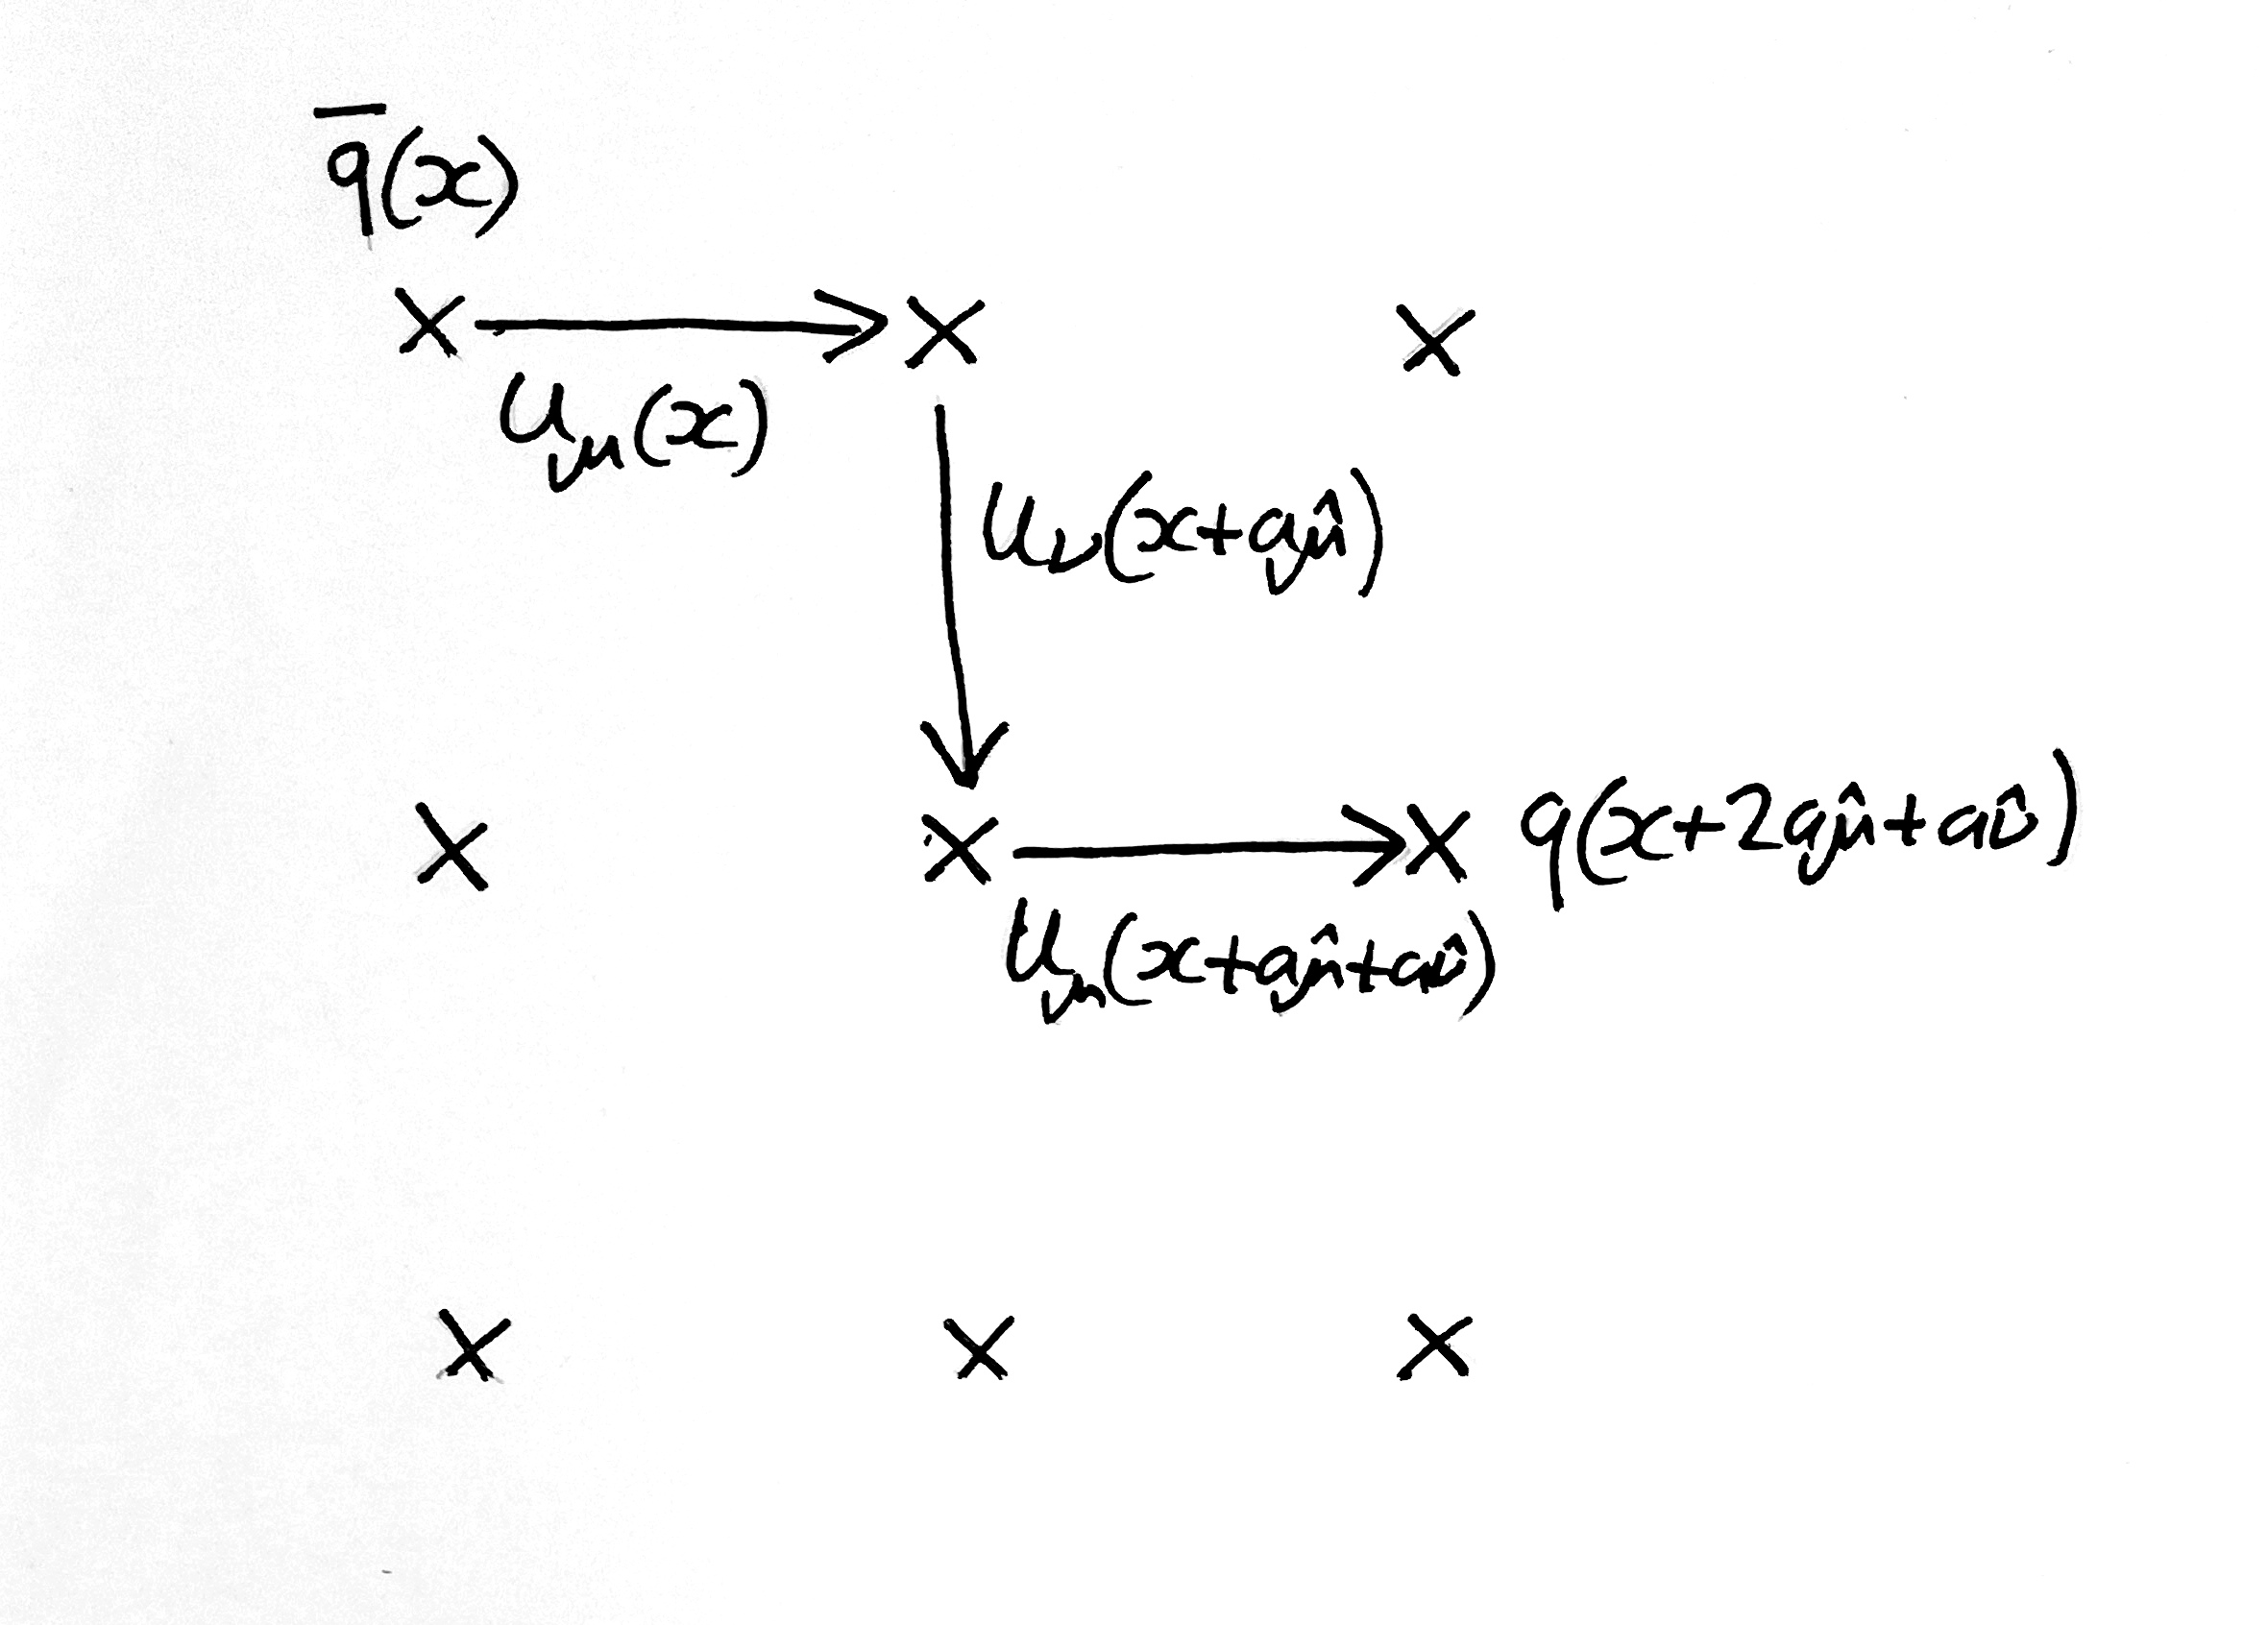
\includegraphics[width=0.55\textwidth]{images/wilson_line.jpg}
    \caption{Depiction of a gauge invariant quark bilinear, connected by a Wilson line made of gauge links.}
  \end{center}
  \vspace{-10pt}
\end{figure}

The $\bar{q}\slashed{D}q$ term in the QCD Lagrangian can then be represented on the lattice in a Gauge invariant way by
\begin{align}
  {1\over 2a}\bar{q}(x) \gamma_{\mu}(U_{\mu}(x)q(x+a\hat{\mu}) + U^{\dagger}_{\mu}(x-a\hat{\mu})q(x-a\hat{\mu}) ).
  \label{eq:latticederivative}
\end{align}
If one defines the links in terms of the the continuum gauge fields $G_{\mu}$ via
\begin{align}
  U_{\mu}(x) = \exp\left( iga G_{\mu}\left(x+{a\hat{\mu}\over2}\right) \right),
\end{align}
then \eqref{eq:latticederivative} takes the correct form in the continuum limit, i.e. it becomes $\bar{q}\slashed{D}q + \order{a^2}$.

\subsection{The Gauge Action}

We must design a pure gauge part of the action in terms of link variables. It is clear that the only gauge-invariant operator that depends only on the link variables are closed loops of links, as in fig. \ref{fig:plaquette}.

\begin{figure}[htb!]
  \begin{center}
    \vspace{-10pt}
    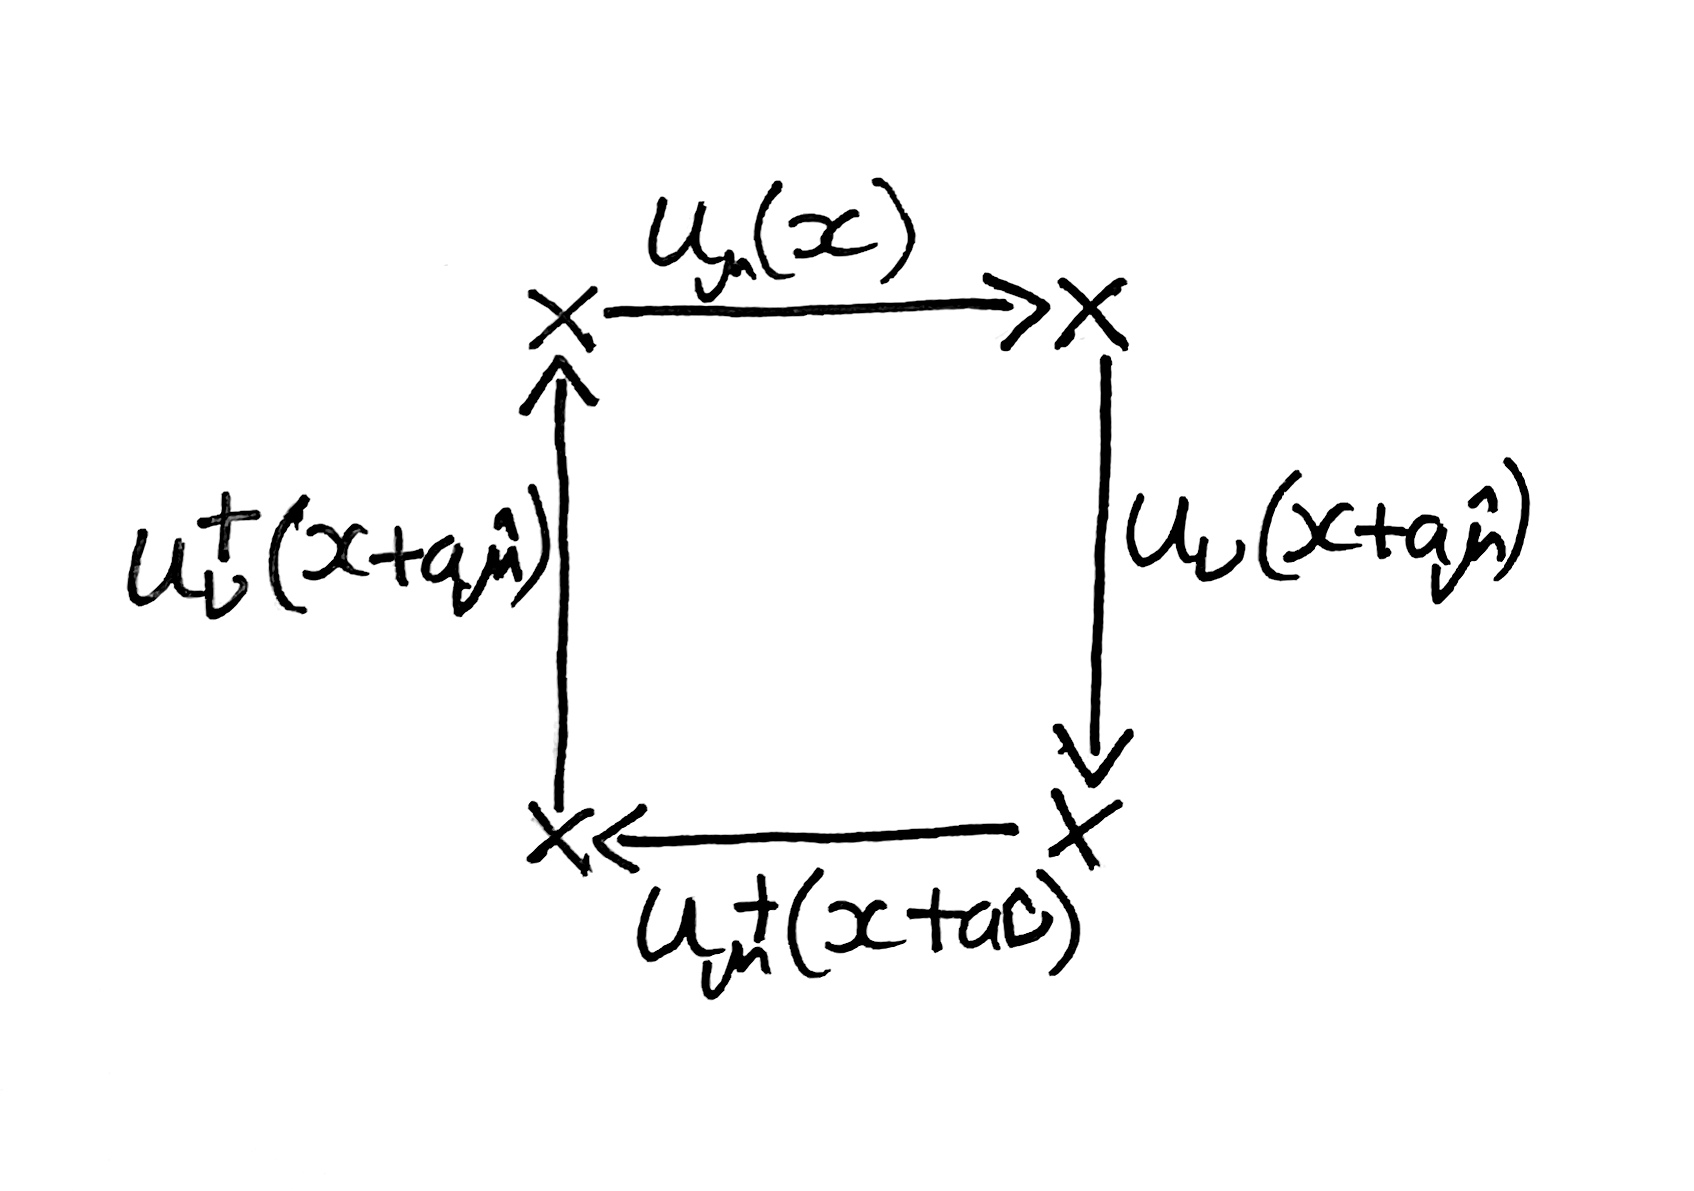
\includegraphics[width=0.55\textwidth]{images/plaquette.jpg}
    \vspace{-15pt}
    \caption{Elementary Plaquette. \label{fig:plaquette}}
  \end{center}
\end{figure}

This brings us basically all the way to a legitimate lattice gauge action. The simplest lattice discretisation of the Yang-Mills action is the real part of the smallest possible closed loop of gauge links;
\begin{align}
  S_G = - &{1\over g^2} \sum_x \sum_{\mu\neq \nu} \text{Re Tr} (1-\Box_{\mu\nu}(x)), \\
  &\Box_{\mu\nu} = U_{\mu}(x)U_{\nu}(x+a\hat{\mu}) U^{\dagger}_{\mu}(x+a\hat{\nu}) U^{\dagger}_{\nu}(x).
  \label{eq:wilson_gauge_action}
\end{align}
$\Box_{\mu\nu}$ is called the {\it{elementary plaquette}}. In the continuum limit this action reduces to
\begin{align}
  S_G = {1\over 4} \int d^4x \text{Tr}G_{\mu\nu}G^{\mu\nu} + \order{a^2},
\end{align}
as required.

%This lattice action can be understood in terms of the geometrical interpretation of gauge theory. The gauge force is due to {\it{curvature}} in the gauge field, a path-dependence in parallel transport. 

In fact, any closed loop reduces to the Yang-Mills action in the continuum. This can be seen intuitively, taking the continuum limit means shrinking any closed loop into an infinitesimally small point. We can choose a gauge action made of any combination of closed loops, so what is the optimal choice?

\subsection{Symmanzik Improvements of the Gauge Action}
\label{sec:symmanzik_gauge}

Any lattice action is admissible for a calculation as long as it reduces to the appropriate QCD action in the continuum. This gives us a lot of freedom in how we chose our lattice action. %A pure gauge action can be any combination of closed Wilson loops.

This freedom can be exploited in order to push expectation values of observables on the lattice closer to their continuum values (reduce the 'discretisation effects'). %such that if one needed to perform an extrapolation of some expectation value to the continuum, the extrapolation would be better controlled.
This program is known as {\it{Symmanzik improvement}}.

In general, a sensible lattice action can be written as
\begin{align}
  S = \sum_{i} c_i \mathcal{O}^i_{\text{lat}} = z_0(\{c_i\}) S_{\text{cont}} + a^2 \sum_{n=1} z_n(\{c_i\}) S_n\,,
  \label{eq:continuum_limit_action}
\end{align}
where $S_{\text{cont}}$ is the continuum action. We are free to choose any $\{c_i\}$ such that $z_0(\{c_i\}) = 1$. In every example we are concerned with, $\order{a}$ terms are absent, so we ignore them here (the arguments presented here carry straightforwardly to situations with $\order{a}$ corrections). A fundemental postulate of the Symmanzik approach is that improvement of one observable (removal of discretisation effects) results in improvement of all other observables. With this in mind, a reasonable approach is:
\begin{itemize}
\item
  Choose some set of lattice operators $\{\mathcal{O}^i_{\text{lat}}\}$. The number of operators required $N$ is the number of allowed irrelevant operators in the continuum theory at mass dimension matching the order of $a$ you want to remove. This is because, formally speaking, one needs $N$ tunable $c_i$ values in order to tune $N$ $z_n(\{c_i\})$ values to zero.
\item
  Inspect the continuum limit of the lattice action to find $z_0(\{c_i\})$, enforce $z_0(\{c_i\})=1$.
\item
  Choose some observable $\mathcal{O}$ that can be calculated in both the lattice and continuum theory. Use the remaining freedom in $\{c_i\}$ to remove the leading $a$ dependence in $\langle \mathcal{O}\rangle$ order by order in perturbation theory. i.e., if we write the expectation value as
  \begin{align}
    \langle \mathcal{O} \rangle = \sum_{n,m} a^{2n} g^{2m}\langle \mathcal{O}_{n,m}(\{c_i\}) \rangle,
  \end{align}
  then this amounts to demanding that $\langle \mathcal{O}_{1,m}(\{c_i\})\rangle = 0$, for as many $m$'s as possible.
\end{itemize}

Applying this to pure QCD, this procedure results in the L\"uscher-Weitz action \cite{luscher1985}. First consider the number of operators required. In continuum pure QCD, the only dimension 4 operator is Tr$G_{\mu\nu}G^{\mu\nu}$. There are no dimension 5 operators, hence there can be no $\order{a}$ contribution to the continuum limit of a lattice action. There are three independent dimension 6 operators:
\begin{gather}
  \text{Tr} J_{\mu\nu\rho} J_{\mu\nu\rho} ,\quad
  \text{Tr} J_{\mu\mu\rho} J_{\nu\nu\rho} ,\quad
  \text{Tr} J_{\mu\mu\nu} J_{\mu\mu\nu}, \\
  J_{\mu\nu\rho} = [ D_{\mu}, G_{\nu\rho} ] \nonumber
\end{gather}
Hence we require 3 extra operators in the lattice action to be tuned in order to remove the three contributions from the $a^2$ terms in Eq. \eqref{eq:continuum_limit_action}. The simplest choice is to take the plaquette action \eqref{eq:wilson_gauge_action}, and add all possible Wilson loops contanining 6 links. This set consists of three families related by hypercubic invariance, {\it{rectangles}} (a), {\it{parallelograms}} (b) and {\it{chairs}} (c), depicted in fig. \ref{fig:LuscherWeitz}.

\begin{figure}
  \begin{center}
    \vspace{-10pt}
    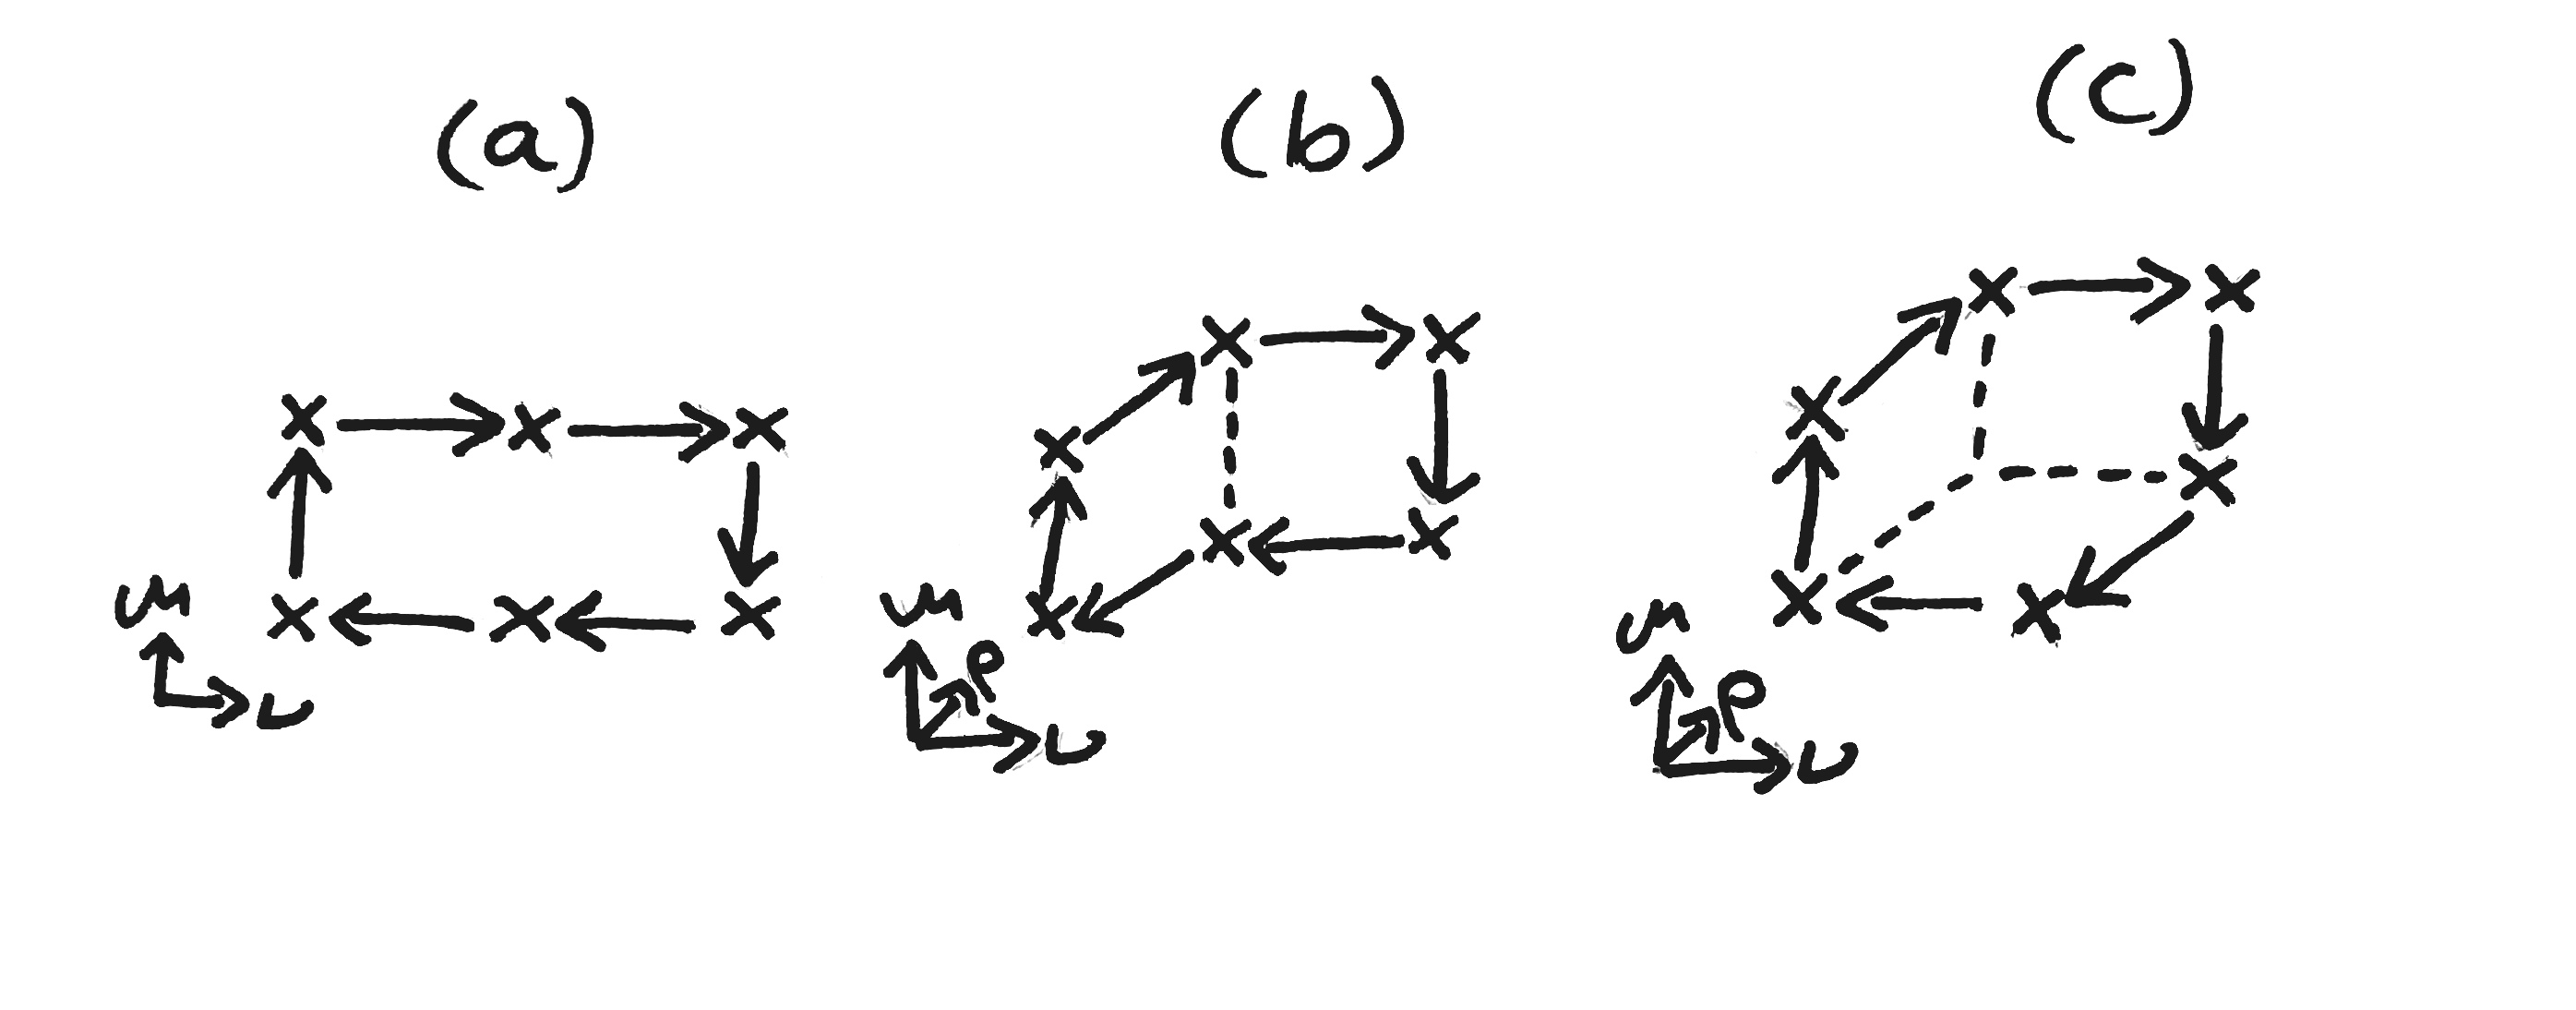
\includegraphics[width=0.85\textwidth]{images/LuscherWeitz.jpg}
    \vspace{-10pt}
    \caption{Terms additional to the elementary plaquette in the improved pure QCD action. \label{fig:LuscherWeitz}}
    \vspace{-10pt}
  \end{center}
\end{figure}

So the new lattice action is
\begin{align}
  S_G =& - {1\over g^2} \sum_x \sum_{\mu\neq \nu}(\quad c_0 \text{Re Tr} (1-\Box_{\mu\nu}(x)) + c_1 \,\text{Re Tr} (1 - \Box^a_{\mu\nu}(x)) \\
  & + \sum_{\rho\neq \mu,\nu}( \,c_2\, \text{Re Tr} (1 - \Box^b_{\mu\nu\rho}(x)) + c_3 \, \text{Re Tr} (1 - \Box^c_{\mu\nu\rho}(x))\quad)\quad)
\end{align}
where $\Box^{a,b,c}_{\mu\nu(\rho)}$ are the Wilson loops in fig. \ref{fig:LuscherWeitz}. Expanding this in small $a$, one finds the function $z_0(\{c_i\})$, setting this to one we find the condition \cite{WEISZ19831};
\begin{align}
  c_0 + 8 (c_1 + c_2) + 16 c_3 = 1.
\end{align}
The rest of the freedom must be fixed by comparing observables in the lattice and continuum theories. In \cite{WEISZ1984397} for example, by matching the gluon propagator between the two theories, one constrains the coefficients further to find
\begin{align}
  c_1 = -{1\over 12} \,,\quad\quad
  c_0 - 8c_3 = {5\over 3}.
\end{align}
These are tree-level relations, so will only prevent lattice artifacts up to $\order{\alpha_s}$. For better improvement, one must compare observables that are sensitive to loop corrections. A popular choice of observable is the so-called static quark potential $V(L)$, this is the potential energy between two static color charges, as a function of separation $L$ between them.
%% It can be related to the expectation value of a rectangular Wilson loop $\Box(L,T)$, extending in one spacial direction by $L$ links and in the time direction by $T$ links. In the $T\to \infty$ limit, this can be written as
%% \begin{align}
%%   \langle \text{Re Tr} \Box(L,T) \rangle \propto \int [d\psi d\bar{\psi} dU] e^{-\sum_x \mathcal{L} + igaA_0 \delta_{{\textbf{x}},{\textbf{x}}_0}  - igaA_0 \delta_{{\textbf{x}},{\textbf{x}}_1} }
%% \end{align}
%% where $\textbf{x}_0$, $\textbf{x}_1$ are two spacial indices $L$ links apart. This can be interpreted as the partition function $Z$ in the presence of two (oppositely charged) static color charges at $\textbf{x}_1$ and $\textbf{x}_2$. From statistical mechanics, the partition function is related to the internal energy of the system via $E = -{1\over T} \ln Z$. This motivates the expression for the static quark potential:
%% \begin{align}
%%   V(L) = - \lim_{T\to \infty} {1\over T} \ln \left( {1\over N} \langle \text{Re Tr} \Box(L,T) \rangle \right),
%% \end{align}
%% where $aN$ is the spacial extent of the lattice. To constrain $\{c_i\}$, one evaluates this order by order in perturbation theory from the continuum and lattice theories, this amounts to comparing $w_n(L,T)$ from the two theories where this is defined by
%% \begin{align}
%%   - \ln \left( {1\over N} \langle \text{Re Tr} \Box(L,T) \rangle \right) = \sum_{n=1}^{\infty} { g_0^{2n} \over (2n)! } w_n(L,T).
%% \end{align}

This procedure is affected by the presence of fermions, so it has been performed a number of times to accommodate different fermion discretisations. In this thesis we report results using the L\"uscher-Weitz action for gauge fields and Highly Improved Staggered Quarks (defined in Sec. \ref{sec:fermions}). The coefficients $\{c_i\}$ were fixed at one-loop %via $w_1(L,T)$
in \cite{Hart:2008sq} to be
\begin{align}
  c_0& = {5\over 3} + ( \,0.237088(46) - 0.1008(34) N_f \,) \alpha_s + \order{\alpha_s^2},\\
  c_1& = -{1\over 12} + ( \,-0.025218(4) + 0.0110(3) N_f \,) \alpha_s + \order{\alpha_s^2},\\
  c_2& = 0 + ( \,-0.04418(4) + 0.0016(3) N_f \,) \alpha_s + \order{\alpha_s^2}, \\
  c_3& = 0.
\end{align}
Since these have been tuned to remove $a^2$ effects up to $\alpha_s$, lattice artifacts in observables computed using this action will be of size $\order{a^2\alpha_s^2}$, so we say this action is $\order{a^2\alpha_s}$-improved.

\section{Lattice Fermions}
\label{sec:fermions}

Putting fermions on the lattice supply a much larger host of complications than gauge fields do. There exist a diverse array of approaches to dealing with fermions on the lattice adopted by different collaborations. Different actions are suited to different types of applications. The plethora of fermion actions is neccesitated by the famous {\textbf{doubling problem}}, which we will describe below.

%In this chapter we will focus only on the fermion actions used in this work; namely the Highly Improved Staggered Quark (HISQ) action, and the Non-Relativistic QCD (NRQCD) action.

Before beginning the discussion of fermion discretisations, we will define some common notation used for gamma matrices in this context. The Euclidian gamma matrices are defined to obey
\begin{align}
  \{\gamma_{\mu},\gamma_{\nu}\} = 2\delta_{\mu\nu}.
\end{align}
These have the useful property $\gamma_{\mu}^2=1$. The full set of spin-mixing matrices can be labelled according to
\begin{align}
  \gamma_n = \prod_{\mu} \left( \gamma_{\mu} \right)^{n_{\mu}}, \quad n_{\mu} = \mathbb{Z}_2.
\end{align}
We implicitly understand the product to be ordered such that $\mu=0$ is the rightmost factor and $\mu=3$ is the leftmost factor. There are 16 such matrices representing corners of the hypercube. One can also use a general site vector $x_{\mu}$ to label the matrix, then $\gamma_x = \gamma_n$ where $n_{\mu} = (x_{\mu}/a)\,\text{mod}\,2$. It is straightforward to show that for any $n$; $\gamma_n^{\dagger} \gamma_n = 1$. We also define $\gamma_{5\mu} = i\gamma_5\gamma_{\mu}$, and $\gamma_{5n} = \prod_{\mu}(\gamma_{5\mu})^n$.

\subsection{The Naive Fermion Action \& The Doubling Problem}

The interacting Dirac action is most naively discretised with
\begin{align}
  S_F &= \sum_{x,\mu} \bar{\psi}(x) \gamma_{\mu} \nabla_{\mu} \psi(x) + m\sum_x \bar{\psi}(x) \psi(x),
  \label{eq:naivefermions}
\end{align}
where $\nabla_{\mu}$ is the gauge covariant finite difference operator,
\begin{align}
  \nabla_{\mu} \psi(x) = {1\over 2a} \left( U_{\mu} (x) \psi(x+a\hat{\mu}) - U^{\dagger}_{\mu}(x-a\hat{\mu})\psi(x-a\hat{\mu}) \right).
  \label{eq:lat_derivative}
\end{align}
%% In appendix \ref{sec:doublingprob} we describe the doubling problem. This is the observation that the propagator for a fermion obeying \eqref{eq:naivefermions}, $M^{-1}(k)$ has the property
%% \begin{align}
%% M^{-1}(k+{\pi\over a}\zeta) = \gamma_{5\mu} M^{-1}(k) \gamma_{5\mu}
%% \end{align}
%% For 16 4-vectors $\zeta_{\mu} \in \mathbb{Z}_2$. This leads to 16 poles in the fermion specturm, therefore 16 distinct excitations (called \textit{tastes}). We require a way of removing the 15 unphysical excitations.
$S_F$ is invariant under a so-called {\it{doubling symmetry}}, which is generated by
\begin{align}
  \label{eq:doublingsymmetry}
  \psi(x) & \to \mathcal{B}_{\mu} \psi(x) \equiv  (-1)^{x_{\mu}/a} \gamma_{5\mu} \psi(x), \\
  \bar{\psi}(x) & \to \bar{\psi}(x)\mathcal{B}^{\dagger}_{\mu} \equiv (-1)^{x_{\mu}/a} \bar{\psi}(x) \gamma^{\dagger}_{5\mu}.
\end{align}
The product space of these form a group of 16 elements $\{\mathcal{B}_{\zeta}\}$, labeled by vectors $\zeta$ with $\zeta_{\mu}\in \mathbb{Z}_2$ (e.g. the element $\mathcal{B}_{0}\mathcal{B}_{1}$ is labeled by $\zeta=(1,1,0,0)$).

The physical significance of this symmetry can be seen when we study its effect on the action. First, notice that
\begin{align}
  \mathcal{B}_{\mu} \psi(x) & = \gamma_{5\mu} \sum_k \tilde{\psi}(k) e^{i(k+{\pi\over a}\hat{\mu})\cdot x} \\
  & = \gamma_{5\mu} \sum_k \tilde{\psi}\left(k-{\pi\over a}\hat{\mu}\right)e^{ik\cdot x},
\end{align}
where $\{k\}$ is a discrete set of 4-momenta, with $k_{\mu}=\pi/an_{\mu}, n_{\mu}\in[1,N_{\mu}]$. The action in momentum space can be written as
\begin{align}
  S = \sum_k \bar{\tilde{\psi}}(k) M(k) \tilde{\psi}(k).
\end{align}
After the operation of $\mathcal{B}_{\mu}$ it becomes
\begin{align}
  S \to \sum_k \bar{\tilde{\psi}}(k) \gamma_{5\mu} M\left(k+{\pi\over a}\hat{\mu}\right)\gamma_{5\mu} \tilde{\psi}(k).
\end{align}
Since we know $S$ is invariant under this transformation, it must be true that $\gamma_{5\mu} M\left(k+{\pi\over a}\hat{\mu}\right)\gamma_{5\mu} = M(k)$, and therefore
\begin{align}
  \boxed{  \quad M^{-1}\left(k+{\pi\over a}\hat{\mu}\right) = \gamma_{5\mu} M^{-1}(k) \gamma_{5\mu}. \quad}
  \label{eq:doubling}
\end{align}
    {\it{This}} it the doubling problem. $M^{-1}$ is the momentum space propagator for the fermion field, so Eq. \eqref{eq:doubling} shows that the spectrum of the fermion is periodic, with a period of $\pi/a$. We expect a pole in $M^{-1}(k)$ where $k \sim m$, $m$ is the pole mass of the fermion. But due to \eqref{eq:doubling} there will now be a second pole at $m + \pi/a$. %This will be around the natural cutoff imposed by the lattice $1/a$, and any higher poles like $m+2\pi/a$ is far above the cutoff so will not contribute.

    Generalizing this argument to all elements of the doubling symmetry, we see that
    \begin{align}
      M^{-1}\left(k+{\pi\over a}\zeta\right) = \gamma_{5\zeta} M^{-1}(k) \gamma_{5\zeta}.
    \end{align}
    This leads to 16 poles in the fermion specturm, one for each $\zeta$ choice, therefore 16 distinct excitations. We cal these excitations \textit{tastes}.

    One can isolate a single taste by a block-scaling procedure. Define
    \begin{align}
      \psi^{(\zeta)}(x_B) = {1\over 16} \sum_{\delta x_{\mu} \in \mathbb{Z}_2} \mathcal{B}_{\zeta}(x_B + \delta x) \psi(x_B + \delta x).
      \label{eq:block-scaling}
    \end{align}
To understand why this only contains one of the tastes, consider the $\zeta = 0$ case. This would only contain the original non-doubler taste since all other poles at $|k|\sim\pi/a$ have been integrated out. For $\zeta \neq 0$, the $\mathcal{B}_{\zeta}$ operator pushes the $\zeta$ doubler to where the $\zeta=0$ taste originally was in $k$ space, then the blocking procedure integrates out the rest.

    %% \begin{figure}
    %%   \vspace{-10pt}
    %%   \begin{center}
    %%     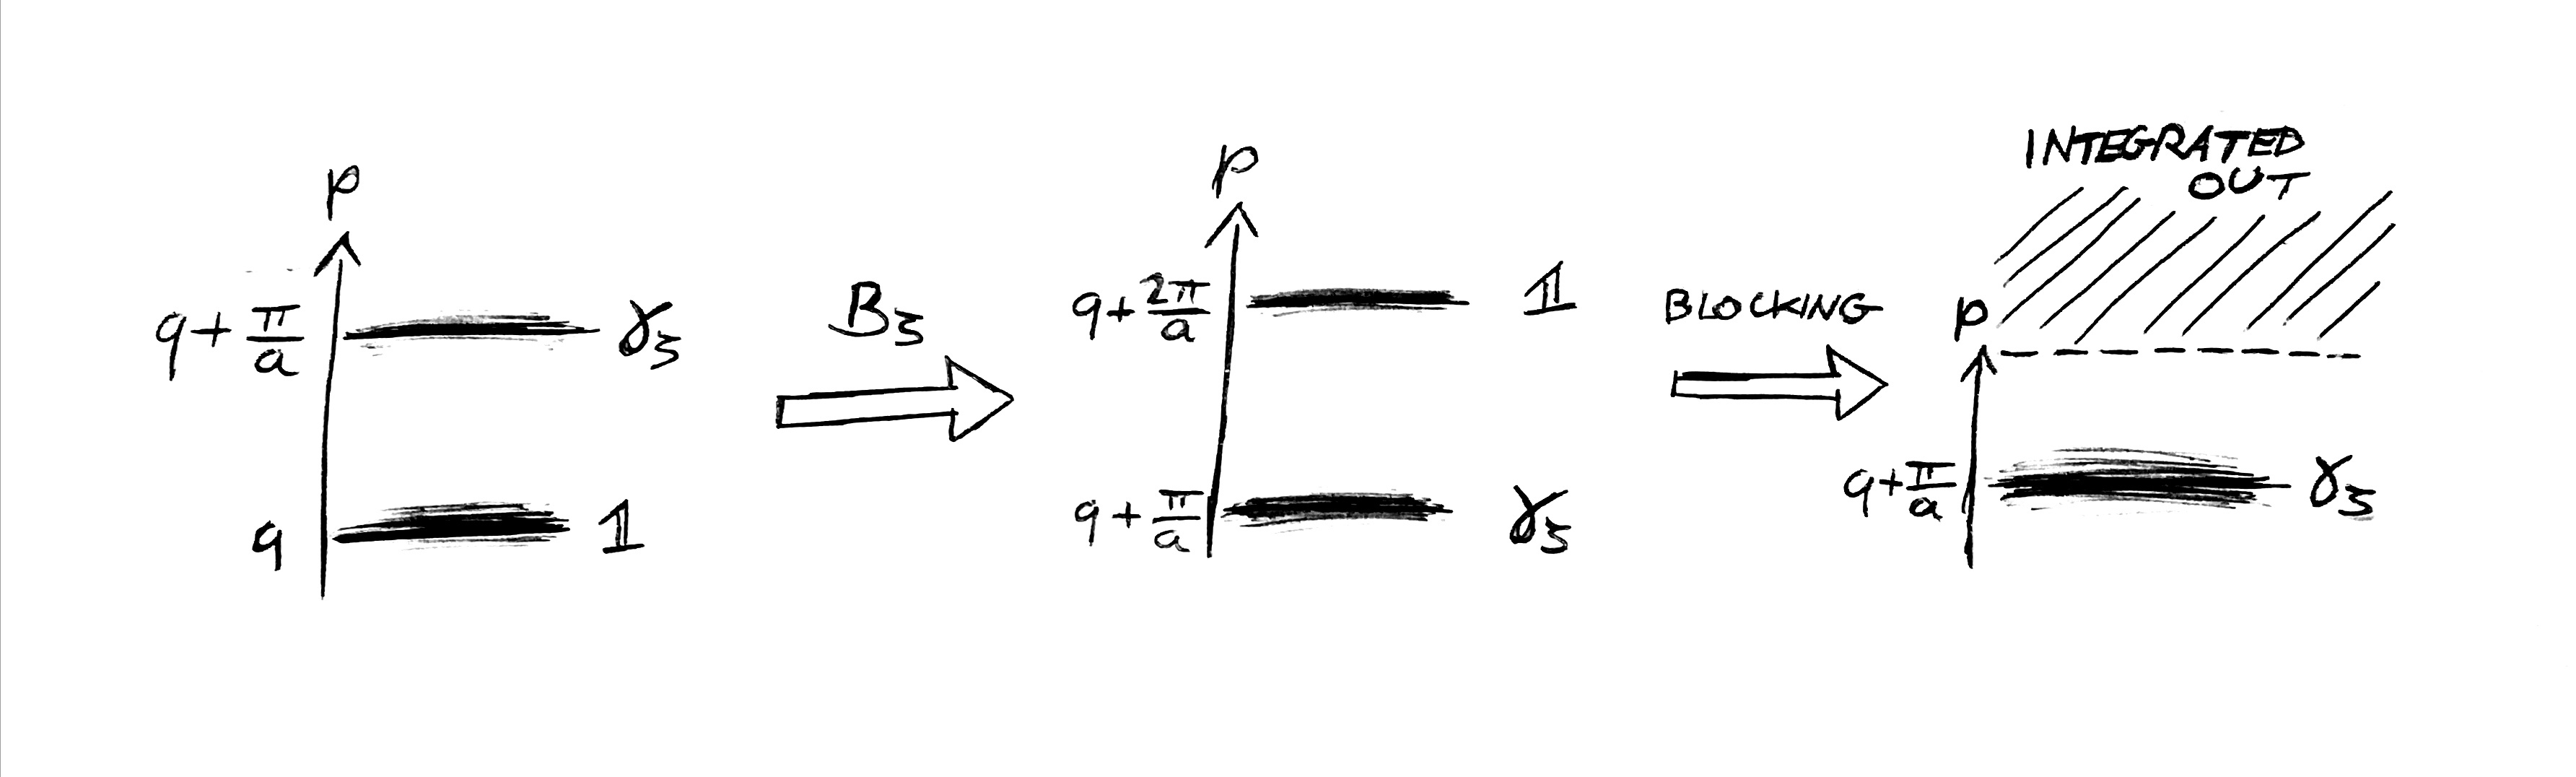
\includegraphics[width=
    %%       1.0\textwidth]{images/blocking.jpg}
    %%   \end{center}
    %%   \vspace{-25pt}
    %%   \caption{Illustration of isolating a single taste via a doubling symmetry transformation $\mathcal{B}_{\zeta}$ then a block-scaling.}
    %%   \label{fig:tastemixing}
    %% \end{figure}

    \subsection{Staggered Quarks}
    \label{sec:staggeredquarks}

    There are a number of solutions to the doubling problem. The most straightforward is to modify the action to push the mass of the unwanted tastes above the momentum cutoff, preventing it from influencing the dynamics. These are called \textit{Wilson-type fermions} \cite{Wilson:1974sk}. However, actions of this type explicitly break Chiral symmetry. Among other issues, this causes additive renormalization of the fermion mass, immensely complicating renormalization procedures.

    Another approach, known as \textit{staggered fermions} \cite{Kogut:1974ag}, partially resolves the doubling issue while retaining a remnant chiral symmetry. The work presented in this thesis makes extensive use of the staggered formalism.
    %Other notable approaches besides Wilson and staggered quarks include \textit{domain wall} \cite{Jansen:1994ym} and \textit{overlap} \cite{Narayanan:2011qj} fermions.

    Staggered fermions are defined via the following. Redefine the fields according to
    \begin{align}
      \psi(x) = \Omega(x) \chi(x),
      \label{eq:staggered}
    \end{align}
    where $\Omega(x)=\gamma_x$. In terms of the new spinor variables $\chi(x)$, the naive action \eqref{eq:naivefermions} becomes
    \begin{align}
      S_F &= \sum_{x,\mu} \bar{\chi}(x)(\alpha_{\mu}(x) \nabla_{\mu} + m ) \chi(x)
    \end{align}
    where $\alpha_{\mu}(x) = (-1)^{\sum_{\nu < \mu} x^{\mu}/a}$. The action is now diagonal in spin, leading to 4 grassman variables with identical actions and identical coupling to the gauge field. As a result, $\chi$ propagators (on fixed gauge backgrounds) are spin-diagonal:
    \begin{align}
      M^{-1}_{\chi}(x,y) = g(x,y) \,\, 1_{\text{spin}},
    \end{align}
    where $g(x,y)$ is a singlet under spin. One need only to include a single component of $\chi$ in a simulation (i.e. fix $\chi = (\chi_1,0,0,0)$), then they can compute $M^{-1}_{\chi}(x,y)[U]$ to obtain $g(x,y)$. Then, using the inverse of Eq. \eqref{eq:staggered}, $g(x,y)$ can be transformed to a propagator of the original spinors:
    \begin{align}
      M_{\psi}^{-1}(x,y) = g(x,y) \,\,\Omega(x)\Omega^{\dagger}(y).
    \end{align}
    This is clearly computationally beneficial, since one only need simulate one spinor component. But also, by only having one spinor component, one reduces the number propagating degrees of freedom by a factor of 4, cutting the number of tastes from 16 down to 4.

    I will show more explicitly how this happens. To do this, consider rewriting an isolated taste (as in Eq. \eqref{eq:block-scaling}) in the staggered formalism, i.e., in terms of $\chi$;
    \begin{align}
      \psi^{(\zeta)}(x_B) = {1\over 16} \sum_{\delta x_{\mu} \in \mathbb{Z}_2} \Omega(\delta x) \mathcal{B}_{\zeta}(0) \chi(x+\delta x).
    \label{eq:chi_blockscale}
    \end{align}
    Recall we set $\chi(x) = (\chi_1(x),0,0,0)$. The product $\Omega(\delta x)\mathcal{B}_{\zeta}(0)$ is simply a product of gamma matrices, so can only serve to ``scramble'' the elements of $\chi$. Then, in the staggered formalism, all 16 tastes $\psi^{(\zeta)}$ amount to only 4 distinguishable fermions: $(\chi_1,0,0,0)$, $(0,\chi_1,0,0)$, $(0,0,\chi_1,0)$, $(0,0,0,\chi_1)$ (with factors of (-1) and $i$).

    To obtain a useful new notation for staggered quarks, we can rewrite Eq. \eqref{eq:chi_blockscale} as
    \begin{align}
      \psi^{\alpha a}(x_B) = {1\over 8} \sum_{\eta_{\mu}\in\mathbb{Z}_2} \gamma_{\eta}^{\alpha a} \chi(x_B+a\eta).
    \end{align}
$\psi^{\alpha a}$ has spin $\alpha$ and taste $a$. Define the {\it{spin-taste}} notation for operators on $\psi^{\alpha a}$ as $(\gamma_n\otimes \gamma_m)$, where $\gamma_n$ acts on the spin component $\alpha$ and $\gamma_m$ acts on the taste component $a$. 

    One can see that the first operator in the spin-taste notation correpsonds to regular spin in the continuum by writing the free fermion action in terms of $\psi^{\alpha a}$:
    \begin{align}
      \nonumber
      S =& \sum_{x_B,\mu} \bar{\psi}(x_B) \left[ (\gamma_{\mu}\otimes 1) \nabla_{\mu} + a ( \gamma_5 \otimes \gamma^*_{\mu} \gamma_5 ) \nabla^{(2)}_{\mu} + {m\over 4}\, (1\otimes 1)  \right] \psi(x_B), \\
      \nonumber
      &\nabla_{\mu}\psi(x_B) = {1\over 4a}\left( \psi(x_B+2a) - \psi(x_B-2a) \right), \\
      &\nabla^{(2)}_{\mu}\psi(x_B) = {1\over 4a^2}\left( \psi(x_B+2a) - 2\psi(x_B) + \psi(x_B-2a) \right).
    \end{align}
If we interpret $(\gamma_{\mu}\otimes 1)$ as a gamma matrix acting on spin in the continuum, we obtain the continuum Dirac action in the $a\to 0$ limit. Including interactions with the gauge field makes the $\order{a}$ term more complicated, but the argument is unchanged.

    Hence, to reproduce some current $\bar{\psi}\gamma_n\psi$ in the continuum, one can use $\bar{\psi}(\gamma_n\otimes \gamma_m)\psi$ on the lattice, where we have the freedom to choose any $\gamma_m$. In terms of $\chi$ fields these look like
    \begin{align}
      \bar{\psi}(x_B)(\gamma_n\otimes \gamma_m) \psi(x_B) = \sum_{\eta,\eta'} \text{Tr} (\gamma_{\eta} \gamma_n \gamma_{\eta'} \gamma_m) \chi^{\dagger}(x_B+a\eta) \chi(x_B+a\eta').
    \end{align}
    The $n=m$ case results in local operators in terms of $\chi$, since the trace will vanish unless $\eta=\eta'$. To build the case with $n\neq m$, one must use 'point-split' operators, i.e. $\chi^{\dagger} (x) \chi(x+\delta x)$.

    In practice in lattice calculations, the remaining 4-fold multiplicity of tastes is tackled in 3 steps:
    \begin{enumerate}
    \item
      Ensure only one taste is created and destroyed at the source and sink of the propagator.
    \item
      Minimize the interaction between tastes by a modification of the action.
    \item
      Remove contributions of extra tastes in the fermion sea by taking det$M \to \sqrt[4]{\text{det}M}$ (the context required to understand this step is eludicated in Sec. \ref{sec:MCMC}).
    \end{enumerate}
    %The third step is the main source of objection to using the staggered formalism for lattice calculations. We will briefly explain this contention in chapter \ref{chap:latticecalculations}.

    %% Step 3 can be justified by the following - in the $a\to 0$ limit, det$M$ tends to (det$M^{(0)})^4$, where $M^{(0)}$ is the Dirac operator for a single taste. Then, taking the 4th root (in principle) reduces the determinant to that of a sea containing 1 taste.

    \subsection{Highly Improved Staggered Quarks}
    \label{sec:HISQ}

    \begin{figure}
      \vspace{-10pt}
      \begin{center}
        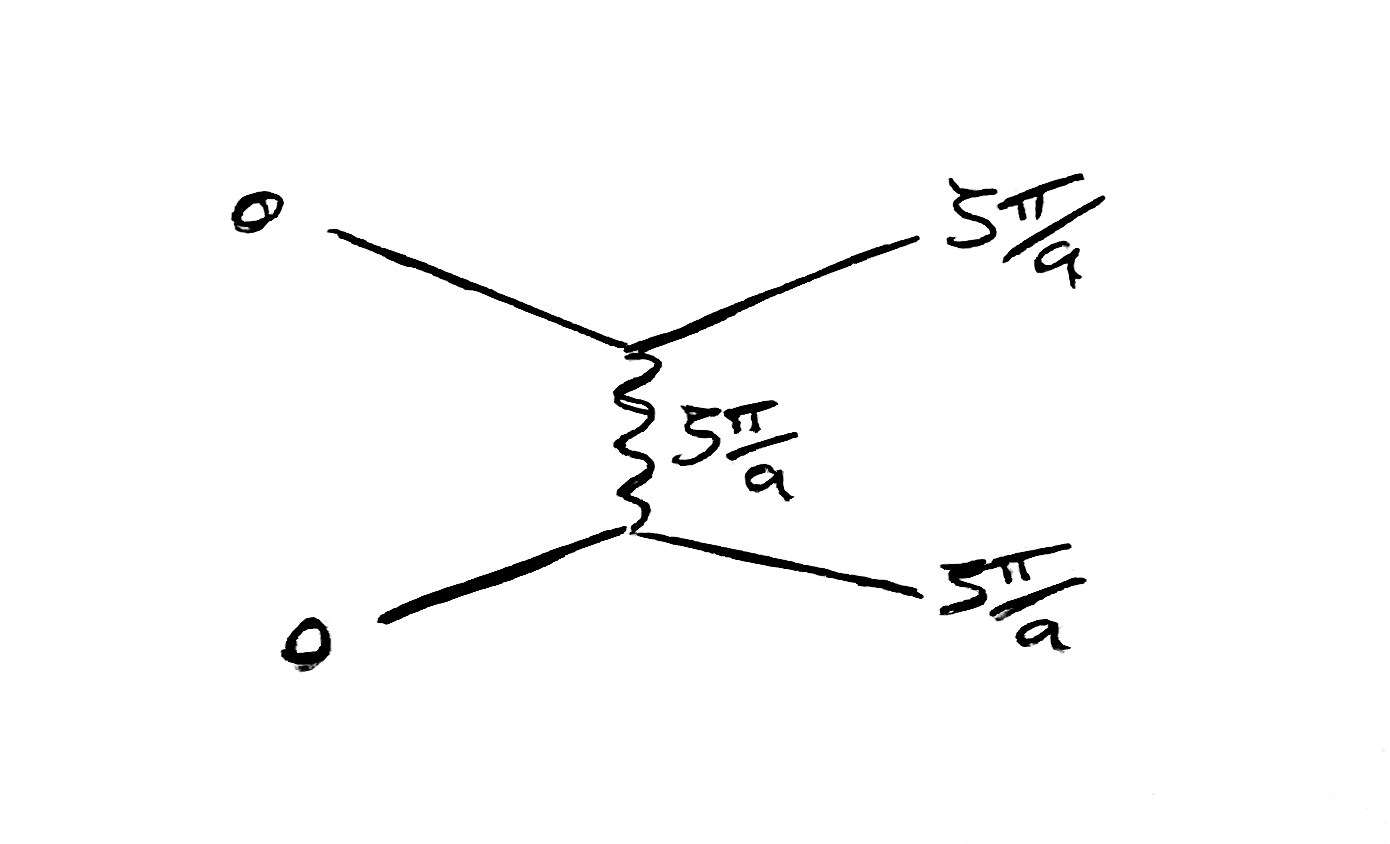
\includegraphics[width=
          0.6\textwidth]{images/taste_exchange.jpg}
      \end{center}
      \vspace{-30pt}
      \caption{Taste mixing at tree level.}
      \label{fig:tastemixing}
    \end{figure}

    Step 2 above is the guiding principle for the action we use in much of this work, the Highly Improved Staggered Quark (HISQ) action \cite{Follana:2006rc}.

    Interaction between different tastes (``taste mixing'') is dominated by the process in fig. \ref{fig:tastemixing}, the exchange of single gluons carrying momenta close to $\zeta \pi/a$. In HISQ, this is suppressed by modifying the gauge fields in such a way as to minimize the coupling between a gluon with momentum ${\zeta\pi/a}$ and the fermions, in other words, minimize the vertices in fig. \ref{fig:tastemixing}.

    To this end, one can change the action so that fermions only couple to {\textit{smeared}} gauge links, in which high-frequency excitations have been removed. Define the first and second covariant derivative operators;
    \begin{align}
      \nonumber
      \delta_{\rho}U_{\mu}(x) & \equiv {1\over a} \big( U_{\rho} (x) U_{\mu} (x + a\hat{\rho}) U_{\rho}^{\dagger}(x+a\hat{\mu}) \\
      & - U_{\rho}^{\dagger}(x-a\hat{\rho})U_{\mu}(x-a\hat{\rho})U_{\rho}(x-a\hat{\rho}+a\hat{\mu})\big),  \\
      \nonumber
      \delta_{\rho}^{(2)} U_{\mu}(x) & \equiv {1\over a^2} \big( U_{\rho}(x) U_{\mu}(x+a\hat{\rho})U^{\dagger}_{\rho}(x+a\hat{\mu}) \\
      \nonumber
      & - 2U_{\mu}(x) \\
      & + U_{\rho}^{\dagger}(x-a\hat{\rho})U_{\mu}(x-a\hat{\rho})U_{\rho}(x - a\hat{\rho} + a\hat{\mu}) \big).
    \end{align}
    With this we can define the smearing operator:
    \begin{align}
      \mathcal{F}_{\mu} = \prod_{\rho\neq\mu} \left( 1 + {a^2 \delta^{(2)}_{\rho}\over 4} \right).
    \end{align}
    HISQ uses two different smeared gauge fields defined by
    \begin{align}
      X_{\mu}(x) &\equiv \mathcal{U} \mathcal{F}_{\mu} U_{\mu}(x), \\
      W_{\mu}(x) &\equiv \left(\mathcal{F}_{\mu} - \sum_{\rho\neq\mu}{a^2(\delta_{\rho})^2\over 2} \right) \mathcal{U} \mathcal{F}_{\mu} U_{\mu}(x).
      \label{eq:gaugesmearing}
    \end{align}
    where $\mathcal{U}$ is a re-unitarization operator, that acts on a matrix $A$ like $\mathcal{U}A = A/\sqrt{A^{\dagger}A}$. The HISQ action can then be written as:
    \begin{align}
{\setlength\fboxsep{10pt} \boxed{\quad      S_{\text{HISQ}} = \sum_{x} \bar{\psi}(x) \left( \sum_{\mu} \gamma_{\mu} \left( \nabla_{\mu}(W) - {a^2\over 6}(1+\epsilon_{\text{Naik}})\nabla^3_{\mu}(X) \right) + m \right) \psi(x) \quad}}
    \end{align}
    Where $\nabla_{\mu}(Z)$ is the covariant derivative \eqref{eq:lat_derivative} with gauge links repaced with $Z$. This action in fact not only removes tree level interactions like fig. \ref{fig:tastemixing}, but also all taste mixing interactions at 1-loop.

    The $\nabla^3_{\mu}$ term is a Symmanzik improvement, it reduces the size of discretisation effects of observables computed using this action. The value of $\epsilon_{\text{Naik}}$ is fixed according to the constraint
    \begin{align}
      \lim_{\underline{p}\to 0} {E^2(\underline{p})-m^2\over \underline{p}^2} = 1.
    \end{align}
    where $E(\underline{p})$ obeys the tree-level dispersion relation from the HISQ action. Tuning $\epsilon_{\text{Naik}}$ according to this constraint gives us the expression
    \begin{align}
      \epsilon_{\text{Naik}} = \,&{ 4 - \sqrt{ 4 + 12 {m_{\text{tree}}\over \cosh(m_{\text{tree}}) \sinh(m_{\text{tree}})} } \over \sinh^2(m_{\text{tree}}) - 1 }, \\
      \nonumber
      m_{\text{tree}} &= m\Big( 1 - {3\over 80}m^4 + {23\over 2240}m^6 + {1783\over 537600 }m^8 \\ &- {76943\over 23654400} m^{10} \Big) + \order{m^{12}}. \nonumber
    \end{align}

    \section{Heavy Quarks on the Lattice}

    The large hierarchy of different quark masses in nature present a number of further complications to lattice calculations. $u$ and $d$ quarks cause huge problems due to how light they are, this will be adressed in Sec. \ref{sec:inversions}. $s$ quarks are easy.

    As quarks get heavier, we begin to encounter another problem. Discretisation effects will generally grow like the largest scale in the theory. If the observable being computed on the lattice is sensitive to the dynamics of a heavy quark of mass $m_h$, this will contain discretisation effects of size $(am_h)^n$ (where $n$ depends on how improved the action is). This is essentially due to the de Broglie wavelength of the heavy quark excitations being close to the lattice spacing, the excitations 'hide' in-between lattice sites.

    How heavy we can go is limited by two factors: the improvement of the lattice action and the lattice spacing. How fine we can get the lattice spacing is limited by computational cost. The physical size of the lattice must always be at least large enough to fit the lightest degrees of freedom in the system, namely it must be larger than the wavelength of pions. This means to get smaller lattice spacing requires increasing the number of sites on the lattice, hence increasing the computational costs (details in chapter \ref{chap:latticecalculations}).

    \begin{figure}
      \vspace{-10pt}
      \begin{center}
        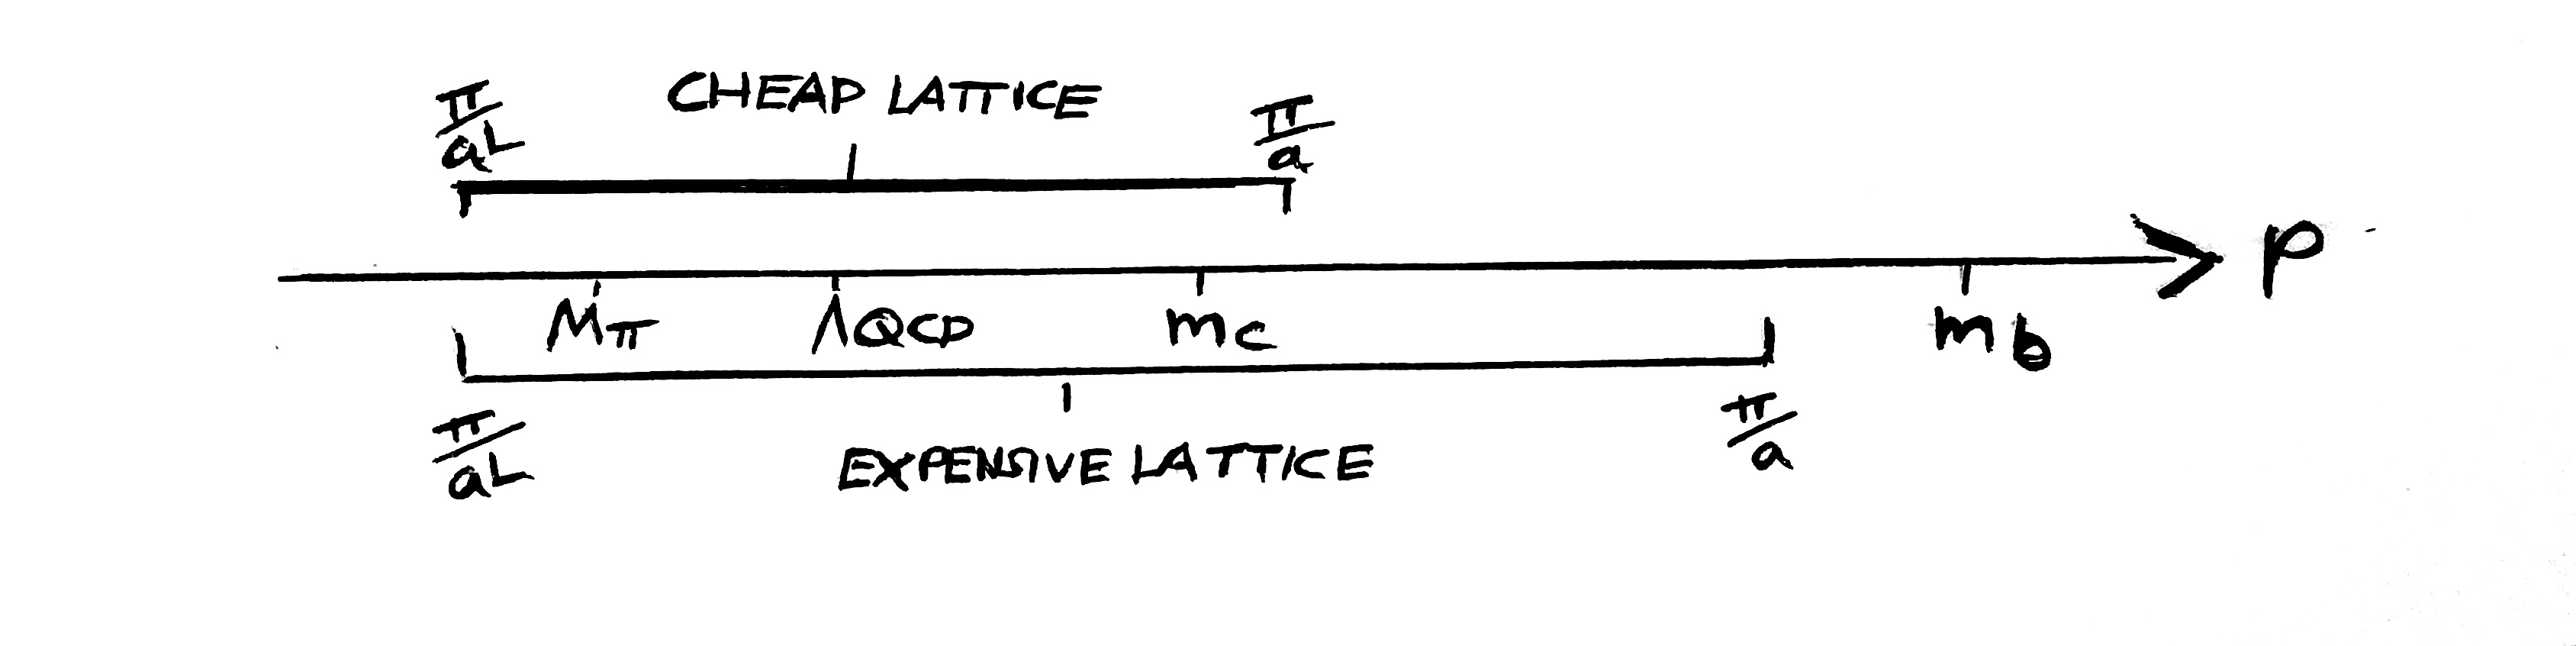
\includegraphics[width=
          0.95\textwidth]{images/scales.jpg}
      \end{center}
      \vspace{-15pt}
      \caption{Different scales relevent to non-perturbative physics, and brackets showing the range of scales that typical lattices can resolve. The larger the range of scales resolved, the more computationally expensive the calculation.}
    \end{figure}

    In the past, $c$ quarks resulted in uncontrollable discretisation effects, but now armed with highly improved actions like HISQ, and very fine lattices, $c$ physics has been conquered on the lattice \cite{Davies:2008nq,Davies:2008hs,Koponen:2011ev,Na:2011mc,Na:2012uh,Na:2012iu,Koponen:2013ila}.

    The mass of the $b$ is still somewhat out of reach. Even with the HISQ action and the finest lattices available with current computational constraints, physical $b$ quarks will create uncontrollable discretisation effects.

    The work in this thesis concerns the decays of mesons containing $b$ quarks. We approach the issue of the heavy $b$ in two different ways, the {\it{heavy-HISQ}} approach, and the {\it{Lattice NRQCD}} approach. Since the main results of this thesis result from our heavy-HISQ studies, we will not go into too much detail in describing lattice NRQCD.

    \subsection{Heavy HISQ}

    The heavy-HISQ approach is essentially to model the $b$ with the HISQ action, but to perform the calculation at a number of unphysically light $b$ masses (that we refer to generically as heavy $h$ quarks), and extrapolate the results to the physical $b$ mass. Typically the $h$ masses span most of the region between the $c$ mass and the $b$ mass.

    Luckily there exists an effective field theory for understanding how to perform such an extrapolation - HQET. HQET gives a framework to describe how observables depend on masses of heavy quarks, so one can use HQET to derive fit forms of such an extrapolation.

    \begin{figure}
      \begin{center}
        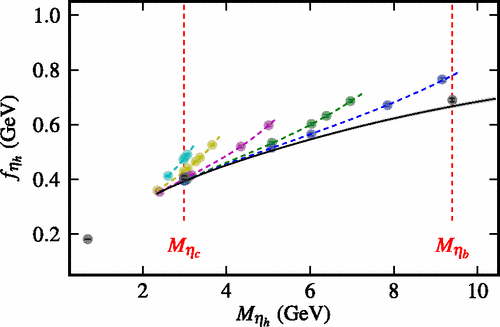
\includegraphics[width=
          0.55\textwidth]{images/fetah_heavyhisq.png}
      \end{center}
      \vspace{-5pt}
      \caption{An extrapolation to $m_h=m_b$ of the $\eta_h$ decay constant (where $\eta_h$ is a pseudoscalar $\bar{h}h$ meson)\cite{McNeile:2012qf}. The colorful points are measurements of $f_{\eta_h}$ on the lattice, the color denotes lattice spacing. The $x$ axis, $M_{\eta_h}$, is a proxy for the $h$-quark mass. \label{fig:McNeile}}
    \end{figure}

    The heavy-HISQ approach is a reasonably new program. It has so far been used for computing $b$ decay constants and masses \cite{McNeile:2011ng,McNeile:2012qf}, and a number of heavy-HISQ calculations of semileptonic form factors are currently underway. The work presented in chapters \ref{chap:BsDsstar} and \ref{chap:BsDs} adopt the heavy-HISQ approach for computing $B_s\to D_s^*l\nu$ and $B_s\to D_sl\nu$ form factors. Besides these, there are also currently ongoing calculations of form factors for the $B_c\to \eta_cl\nu$, $B_c\to J/\psi l\nu$ \cite{Lytle:2016ixw}, $B_c\to B_sl\nu$, $B_s\to \eta_sl\nu$, and $B\to D^*l\nu$ decays.

    \subsection{Lattice NRQCD}

    The root of the problem of heavy quarks on the lattice is in the rest mass of the quark. Consider the expansion in momentum $\textbf{p}^2$ of the continuum relativistic dispersion relation:
    \begin{align}
      \omega = \sqrt{{\textbf{p}}^2 + m^2} \simeq m + {{\textbf{p}}^2\over 2m} - {{\textbf{p}}^4\over 4m^3} + ...
      \label{eq:rel_expansion}
    \end{align}
The rest mass in the first term is the source of the issue, when $m > \pi/a$ the first term pushes the frequency of excitations $\omega$ close to or  over $\pi/a$.

One could replace the relativistic fermion action e.g. HISQ, with a lattice version of NRQCD \cite{Lepage:1992tx}. In NRQCD the $b$ has no rest mass, so $b$ excitations will have frequencies much smaller than $\pi/a$.

    %% The leading order Lagrangian in the continuum is
    %% \begin{align}
    %%   \mathscr{L}^0_{NRQCD} = \psi^{\dagger}_+ \left[ i\partial_0 + {{\bf{\nabla}}^2\over 2m_b} \right] \psi_+.
    %% \end{align}
    %% $\psi_+$ is the first two components of a Dirac spinor, the second two components (the antiparticle) are not present since the dispersion relation from this Lagrangian has no antiparticle solutions.
    %% $m_b$ is the bare mass for the $b$ quark. The NRQCD action reproduces \eqref{eq:rel_expansion} with the first term chopped out.

    %% Correction terms are chosen to be all gauge-invariant terms, grouped according to powers of the quark velocity $v$. For an example of deducing such powers: kinetic enegry = $m_b v^2 = \int d^3x \psi_+^{\dagger} {\bf{\nabla}^2\over 2m_b} \psi_+$ $\rightarrow$ $|\bf{\nabla}|/m_b \sim v$.

    Another benefit of NRQCD is that it does not suffer from a doubling problem, since the doubling problem is a purely relativistic issue (the doubling symmetry requires 4 component spinors for $\gamma$ matrices to act on.

    The lattice calculations we perform require us to compute propagators for $b$ quarks on fixed gauge backgrounds. The form of the action allows propagators $G_b({\textbf{x}},t)[U]$ to be computed using a simple recursion relation
    \begin{align}
      G_b({\textbf{x}},t+1)[U] = e^{-aH}[U] G_b({\textbf{x}},t)[U],
      \label{eq:nrqcd_recursion}
    \end{align}
    which is numerically very fast in comparison to how HISQ propagators are computed (see Sec. \ref{sec:inversions}). $H$ is the NRQCD Hamiltonian. In the interest of numerical stability, the time evolution operator is re-cast as
    \begin{align}
      e^{-aH} = \left(1 - {a\delta H\over 2}\right)\left(1-{aH_0\over 2 n}\right)^n U_0^{\dagger}({\textbf{x}},t) \left(1 - {aH_0\over 2n}\right)^n \left(1-{a\delta H\over 2}\right),
    \end{align}
    where $n$ is an arbitrary integer (chosen in our studies to be $n=4$), and the Hamiltonian has been broken up into a leading part $H_0$ and correction $\delta H$. $G_b$ here are propagators for the 2-component spinor fields used in NRQCD (see Sec. \ref{sec:continuum_nrqcd}). We use the $\mathcal{O}(\alpha_s v^4)$ corrected NRQCD Hamiltionian:
    \begin{align}
      aH_0 =& - {\nabla^{(2)}\over 2am_b} , \\
      \nonumber
      a\delta H =& - c_1 {(\nabla^{(2)})^2 \over 8 (am_b)^3} + c_2{ i\over 8(am_b)^2} ( \nabla\cdot {\bf{\tilde{E}}} - {\bf{\tilde{E}}}\cdot \nabla) \\
      \nonumber
      & - c_3 {1\over 8(am_b)^2} \sigma\cdot ( \nabla\times{\bf{\tilde{E}}} - {\bf{\tilde{E}}}\times\nabla) \\
      \nonumber
      & - c_4 {1\over 2am_b} \sigma\cdot {\bf{\tilde{B}}} + c_5 {\nabla^{(4)}\over 24 am_b} \\
      & - c_6 {(\nabla^{(2)})^2\over 16n (am_b)^2},
      \label{eq:nrqcd_dH}
    \end{align}
    where $\nabla^{(2,4)}$ are the second and fourth lattice derivative, $\sigma$ are $SU(2)$ matrices acting on spin, and ${\bf{\tilde{E}}}$ and ${\bf{\tilde{B}}}$ are the (Symmanzik improved) chromoelectric and chromomagnetic fields. The form of $\nabla^{(2,4)}$,${\bf{\tilde{E}}},{\bf{\tilde{B}}}$ were defined in Sec. 4.2 of \cite{Lepage:1992tx}, and were improved upon in \cite{Gray:2005ur}.

    The coefficients $\{c_i\}$ have been fixed via various calculations adopting a number of methods. The coefficients of the kinetic terms, $c_{1,5,6}$, were most recently fixed by comparing the lattice NRQCD dispersion relation to that of the continuum in perturbation theory \cite{Davies:2018fwg}. $c_2$ is a spin-independent term which can effect radial and orbital excitation energies, this is not expected to have as large an effect as the kinetic terms, so is set to its tree-level value of 1. The result of varying $c_2$ on relevant observables was investigated in Sec. IIIC of \cite{Dowdall:2011wh}, and the effects were very small. $c_3$ and $c_4$ are spin-dependent terms, which would have a small effect on spin-averaged observables (i.e. all observables computed in this work). $c_3$ is set to 1, and $c_4$ is tuned non-perturbatively, by matching predictions of the fine structure of the $\Upsilon$ spectrum from lattice NRQCD to experiment \cite{Dowdall:2011wh}.

Another symmanzik improvement is introduced in this context by multiplying the gauge links by the so-called {\textit{tadpole factor}} $u_0 = \sum_{\mu,\nu}\langle \text{Tr}\Box_{\mu\nu} /4\rangle$. This removes the tadpole diagrams proportional to $a^2$ that appear in gluon propagators.
    
    Once the propagator for the 2-component non-relativistic $b$ quark has been found, it must be transformed back into a 4-component spinor. This is done by an inverse Fouldy-Wouthuysen transformation \cite{PhysRev.78.29}:
    \begin{align}
      \psi(x) = e^{-{{\bf{\gamma}}\cdot{\bf{D}}\over 2m_b}}\binom{\psi_+(x)}{0}.
      \label{eq:FoldyWoldy}
      \end{align}
 % lattice qcd
\chapter{Lattice Calculations}
\label{chap:latticecalculations}

The previous chapter focused on how to discretize the QCD action. This chapter is focused on the practical side of lattice QCD - given a lattice action, how does one perform the functional integral to determine expectation values?

\section{Evaluation of Lattice Correlation Functions}
\label{sec:latpathint}

All physics of a quantum field theory can be extracted from correlation functions. So a typical lattice calculation involves computing a correlation function (or just {\it{correlator}}) on the lattice, then extracting physical quantities from it. A typical correlator that is computed on the lattice is a 2-point meson correlator, i.e. $\langle\Phi(x)\Phi^{\dagger}(y)\rangle$ where $\Phi$ is a meson creation operator and $\Phi^{\dagger}$ is an annihilation operator. This is a good working example for showing the steps in a lattice calculation, the generalization to $N$-point correlators is reasonably natural.

A creation/annihilation operator for a meson in this context can be any operator containing the same quantum numbers as the meson one is studying. For example, the neutral $B$ meson is a pseudoscalar charged with a $b$ and $\bar{d}$ quark, so a suitable operator is $\Phi(x) = \bar{b}(x)\gamma_5 d(x)$. The corresponding functional can then be written as
\begin{align}
  \nonumber
  C(x,y) = \langle \Phi(x)\Phi^{\dagger}(y)\rangle =& \int [d\psi d\bar{\psi} dU] \left(\, \bar{b}(x)\gamma_5 d(x) \bar{d}(y)\gamma_5 b(y) \text{ }\right) \\&\times \exp\left(-S_G[U]-\sum_{w,z,i} \bar{q}_i(w)M_{q_i}(w,z)[U]q_i(z)\right),
\end{align}
where we have broken the action up into a gauge part $S_G[U]$, and a fermion part. $M_{q_i}(x,y)[U]$ is the Dirac operator for flavour $i$, and can be seen as a matrix in lattice site, color and spin.

The integral over fermions can be performed analytically since the fermion fields are Grassman valued. In our example, the result is \cite{Peskin:1995ev}:
\begin{align}
  \nonumber
  C(x,y) = \int [dU]\, &\text{Tr}\left( \, M^{-1}_b(y,x)[U] \, \gamma_5 \, M^{-1}_d(x,y)[U] \, \gamma_5 \, \right) \\ &\times e^{-S_G[U]} \prod_i\text{det}(M_{q_i}[U])\,.
  \label{eq:lattice_correlator}
\end{align}
The quantinties $M_{q_i}^{-1}(x,y)[U]$ are propagators of a quark of flavour $q$ on a fixed gauge background $U$. For clarity: here $U$ denotes a configuration of angles comprising an $SU(3)$ matrix for each element of the set of all links on the lattice $\{ U_{\mu}(x) | \,\forall \,\mu,\,x \}$. The trace is over color and spin. The integration over gauge fields is generally carried out by an importance sampling method. A finite \textit{ensemble} of gauge configurations $\{U_n\}$ is generated by a Monte Carlo Markov Chain (MCMC), where the probability of a gauge configuration $U_n$ being added to the ensemble is proportional to
\begin{align}
  p(U_n) = e^{-S_G[U_n]}\prod_i\text{det}(M_{q_i}[U_n]).
  \label{eq:MCweight}
\end{align}

Once the ensemble is created, the path integral can be approximated by simply
\begin{align}
  C(x,y) \simeq {1\over N} \sum^N_{n=1} \text{ Tr}\left[\text{ } M^{-1}_b(y,x)[U_n] \gamma_5 M^{-1}_d(x,y)[U_n] \gamma_5 \text{ }\right]\,,
  \label{eq:av_gauge}
\end{align}
where $N$ is the number of configurations in the ensemble. This introduces a statistical error that scales like $1/\sqrt{N}$. The calculation of the correlation function then is split into 3 steps:
\begin{enumerate}
\item
  Generate an ensemble of gauge configurations $\{ U_i \}$ by MCMC (Sec. \ref{sec:MCMC}).
\item
  Compute $M^{-1}_{q_i}(x,y)[U]$ by inverting the Dirac operator on each gauge configuration (Sec. \ref{sec:inversions}).
\item
  Construct the trace in Eq. \eqref{eq:av_gauge}, and average over the ensemble. This step is dealt with in the context of staggered quarks in Sec. \ref{sec:staggeredcorrelators}.
\end{enumerate}


\subsection{Generation of Gauge Ensembles}
\label{sec:MCMC}

The calculation requires a number of samples of gauge configurations $\{U_n\}$ sampled from the distribution $p(U)$ defined in Eq. \eqref{eq:MCweight}. In this section (Sec. \ref{sec:MCMC}) I largely follow the discussion given in \cite{DeGrand:2006zz}.

The physical interpretation of the determinant in \eqref{eq:MCweight} is that it accounts for virtual quark loops in gluon propagators. In the early days of lattice calculations, this determinant was approximated to 1, since its evaluation was an insurmountable computational cost, and it was expected that sea quarks had small effects on observables (this is known as the {\it{quenched approximation}}). However, this introduced large systematic effects that could not be well controlled. These days, our computational ability has improved and sophisticated approaches to computing the determinant have been developed (e.g. \cite{PhysRevD.35.2531}), so we can include it in our calculations.

We will roughly follow the history of gauge ensemble generation, by first ignoring the determinant, and then showing how it is eventually included in the process.

\subsubsection{Quenched MCMC}

Gauge ensembles are generated via an MCMC, inspired by statistical mechanics. The distribution exp$(-S_G[U])$ is suggestive of something like a Boltzmann distribution for a gas of particles, each with some state $U_i$, in thermal equilibrium. The ergodic hypothesis states that a single particle in this gas will jump between possible states over time such that, at any given time, its probability of being in state $U_i$ is given by exp$(-S_G[U_i])$. In MCMC, one starts with some random state $U_0$, then repeatedly updates the state according to some update rule or `hopping rate' $p(U_i\to U_j)$. 

The hopping rate must be designed to bring the chain into thermal equilibrium with the correct distribution. A sufficient condition for thermal equilibrium is known as {\it{detailed balance}}, where the probability of jumps between any pair of states $i$ and $j$ is equal:
\begin{align}
  p(U_i) p(U_i\to U_j) = p(U_j) p(U_j\to U_i)\,.
\end{align}
Hence $p(U_i\to U_j)$ must be designed according to the rule
\begin{align}
  {p(U_i\to U_j) \over p(U_j\to U_i)} = \exp(-(S_G[U_i]-S_G[U_j]))\,.
  \label{eq:detailed_balance}
\end{align}
There are a number of possible choices of how to design $p(U_i\to U_j)$. One approach, called {\bf{molecular dynamics}} \cite{PhysRevLett.49.613,PhysRevD.28.1506} is to model the chain as the trajectory $U(\tau)$ of a system with Hamiltonian
\begin{align}
  H(\pi,U) = {\pi^2\over 2} + S_G[U]\,,
\end{align}
where $\pi$ is a fictitious momentum conjugate to $U$. It can be demonstrated that such a trajectory obeys \eqref{eq:detailed_balance} \cite{PhysRevLett.49.613}. The trajectory is computed via Runge-Kutta numerical integration. One may worry about the possibility of fixed points, limit cycles etc. in the dynamics, which would prevent ergodicity. To avoid this one can introduce a periodic {\bf{refreshing}} step, where $\pi$ assigned a new value from normally distributed noise \cite{PhysRevLett.55.2774,duane1986}.

Another problem that can occur in molecular dynamics is when errors in Runge-Kutta iterations accumulate over time. Diversion from the dynamics enforced by $H(\pi,U)$ can ruin the ergodicity of the trajectory. To fix this, one can add a {\bf{Metropolis}} step at regular intervals $\delta\tau$ throughout the evolution \cite{doi:10.1063/1.1699114}. In this step, one either accepts (continues onto the next stage of molecular dynamics) or rejects (refreshes $\pi$ and re-calculates the $\delta \tau$ worth of molecular dynamics), according to the criterion
\begin{itemize}
\item
  If $S_G[U(\tau+\delta\tau)] < S_G[U(\tau)]$, always accept.
\item
  Otherwise, accept if $\,\exp\left(S_G[U(\tau+\delta\tau)] - S_G[U(\tau)]\right) > \lambda$, where $\lambda$ is randomly chosen from the interval $[0,1]$.
\end{itemize}
The metropolis step ensures detailed balance (Eq. \eqref{eq:detailed_balance}) is satisfied even in the presence of Runge-Kutta errors.

The combination of molecular dynamics, refreshing steps and Metropolis steps is referred to as {\bf{Hybrid Monte Carlo}} \cite{DUANE1987216}, and is the basic method of how the ensembles we use in this thesis were generated. I now address how the determinant det$M$ is included.

\subsubsection{Unquenched MCMC}

Simply evaluating det$M[U]$ directly, given a configuration $U$, is prohibitively expensive due to the non-local nature of the determinant. Recall $M[U]$ is a matrix in spin, colour, and lattice site, in modern calculations this will have a dimension of order $10^8$. Even holding that much information in memory is not feasible. A solution to this is to use the $\Phi$-algorithm \cite{PhysRevD.35.2531}.

First, we replace det$M$ with det$M^{\dagger}M$. If we were only including $u$ and $d$ quarks in the sea, this would be fine since we can approximate $u$ and $d$ to be two degenerate flavours, then $\prod_q \det M_q = \det M \det M = \det M^{\dagger} M$. In the case of an arbitrary set of flavours, this requires a correction that will be addressed later.
The $\Phi-$algorithm involves introducing new artificial scalar fields $\Phi(x)$ and $\Phi^{\dagger}(x)$ via
\begin{align}
  \det M^{\dagger} M = \int [d\Phi^{\dagger}d\Phi] \exp(-\Phi^{\dagger} (M^{\dagger}M)^{-1}\Phi).
\end{align}
then one can add $\Phi^{\dagger} (M^{\dagger}M)^{-1}\Phi$ to $S_G$ in the Hybrid Monte Carlo algorithm. The extra functional integral over $\Phi,\Phi^{\dagger}$ is easly evaluated, by sampling a vector $\eta$ from a normal distribution exp$(-\eta^{\dagger}\eta)$, then transforming it to $\Phi = M^{\dagger} \eta$.

\subsubsection{The Rooting Trick}

We will now address how to correct for the fact that we have replaced det$M$ with det$M^{\dagger}M$ in the presence of arbitrary non-degenerate flavours. We have explicitly doubled the fermions to two degenerate flavours per physical flavour. In the case of staggered quarks, this is not a huge marginal complication since we already have four degenerate tastes which we have to deal with anyway. In order to cut down the number of tastes in the sea, the solution is to take the fourth-root of det$M$. When using the $\Phi$-algorithm, this becomes the 8th root of det$M^{\dagger}M$.
\begin{align}
  (\det M^{\dagger} M )^{1/8} &= (\prod_i \lambda_i^2)^{1/8} = (\prod_i \lambda_i)^{1/4} \\ \nonumber &\stackrel{?}{=} (\prod_i\lambda_i^{'\,4})^{1/4} = \prod_i \lambda'_i \quad (a\to 0).
\end{align}
where $\lambda_i$ are eigenvalues of $M$. On the second line, we have assumed that the matrix $M$ can be decomposed into four matrices, one for each of the four tastes, with eigenvalues $\lambda'_i$ which are degenerate in the continuum limit.

This assumption is not rigorously justified in field theory, so the fourth-root trick is a source of controversy. Much has been said about the problems this may cause in lattice results \cite{JANSEN20043,CREUTZ2007230,Creutz:2007rk}, however, these concerns have been refuted \cite{Kronfeld:2007ek,Sharpe:2006re}. It has been demonstrated that the eigenvalues smoothly become degenerate as one approaches the continuum limit \cite{Follana:2004sz,Donald:2011if}.
There has so far emerged no evidence that the rooting trick is harmful, observables computed using unquenched staggered quarks have always agreed with experiment, analytical approaches (e.g. \cite{Durr:2012te}), and other lattice discretisations. 

Introducing the $1/2$ or $1/8$th root to the determinant requires a modification of the $\Phi$-algorithm, we can no longer simply sample $\Phi$ using $\Phi=M^{\dagger}\eta$. The effective action is now $S_G + \Phi^{\dagger} (M^{\dagger}M)^{-1/8} \Phi$. The root is dealt with by replacing it with a partial fraction representation \cite{Clark:2006fx}:
\begin{align}
  (M^{\dagger}M)^{-1/8} \simeq a_0 + \sum_{n=1}^N { a_n \over M^{\dagger}M + b_n }.
  \label{eq:rational}
\end{align}
This can only be evaluated by some variation of a conjugate gradient algorithm (specifically a multishift solver \cite{Frommer:1995ik,Jegerlehner:1996pm}). Conjugate gradient will be described in Sec. \ref{sec:inversions}. This approach is called the {\bf{Rational Hybrid Monte Carlo}} (RHMC) algorithm.

\subsubsection{The $N_f=2+1+1$ MILC Ensembles}
\label{sec:MILCensembles}

In this work, we use ensembles of gauge configurations generated by the MILC collaboration \cite{Bazavov:2012xda,Bazavov:2010ru}. The ingredients of these configurations are
\begin{itemize}
\item
  Gauge fields obeying the one-loop Symanzik improved L\"uscher-Weisz action described in Sec. \ref{sec:symanzik_gauge}.
\item
  Four flavours of quark in the sea, $u$,$d$,$s$ and $c$ (with $m_u=m_d\equiv m_l$), hence the notation $N_f=2+1+1$, obeying the HISQ action, described in Sec. \ref{sec:HISQ}.
\item
  Ensemble generated (mostly) using the RHMC algorithm as described earlier in this section. Some configurations on set 3 were instead generated using an RHMD algorithm - similar to RHMC except with the Metropolis accept/reject step omitted.
\end{itemize}
Table \ref{tab:ensembles} gives the details of the MILC ensembles that were used in this work. One may notice that for the majority of ensembles here, the light quarks are much heavier than in reality. The necessity for this is explained in the next section.

\begin{table*}[t]
  \begin{center}
    \begin{tabular}{c c c c c c c c c c}
      \hline
      set & name & $w_0/a$  & $N_x^3\times N_t$ & $am_{l0}$ & $am_{s0}$ & $am_{c0}$  \\ [0.5ex]
      \hline
      0 & \bf{very coarse} & 1.1119(10) & $16^3\times48$ & 0.013 & 0.067 & 0.838 \\ [1ex]
      1 & \bf{coarse} & 1.3826(11) & $24^3\times64$ & 0.0102 & 0.0509 & 0.635 \\ [1ex]
      2 & \bf{fine} & 1.9006(20) & $32^3\times96$ & 0.0074 & 0.037 & 0.440 \\ [1ex]
      3 & \bf{fine-physical} & 1.9518(7) & $64^3\times96$ & 0.0012 & 0.0363 & 0.432 \\ [1ex]
      4 & \bf{superfine} & 2.896(6) & $48^3\times144$ & 0.0048 & 0.024 & 0.286 \\ [1ex]
      5 & \bf{ultrafine} & 3.892(12) &  $64^3\times192$ & 0.00316 & 0.0158 & 0.188  \\ [1ex]
      \hline
    \end{tabular}
  \end{center}
  \caption{Parameters for the MILC gluon ensembles \cite{Bazavov:2010ru,Bazavov:2012xda}. $a$ is the lattice spacing, determined from the Wilson flow parameter $w_0$. Values for $w_0/a$ are from: sets 0,1,2 \cite{Chakraborty:2016mwy}, sets 3 and 4 \cite{Chakraborty:2014aca}, set 5 \cite{mcneile:private}. The physical value of $w_0$ was determined to be $w_0=0.1715(9)$fm in \cite{Dowdall:2013rya}. Columns 5-7 give the masses used in the action for light,strange and charm quarks in the sea. \label{tab:ensembles}}
\end{table*}


\subsection{Dirac Operator Inversion}
\label{sec:inversions}

Once the ensemble $\{U_i\}$ has been generated, to compute the 2-point correlator \eqref{eq:av_gauge} one must compute $M^{-1}[U_i]$ for each $U_i$. We have already seen how this can be done in the case of the flavour in question being governed by the NRQCD action, one can use the recursion relation \eqref{eq:nrqcd_recursion}. In the case of relativistic actions like HISQ, there is no equivalent recursion relation.

$M$ is large but sparse. It technically has $\order{\text{Vol}^2}$ elements, but for suitably local actions (like HISQ) it has only $\order{\text{Vol}}$ non-zero elements. This means it is well-suited to the {\bf{conjugate gradient}} (CG) algorithm \cite{Hestenes&Stiefel:1952} (and its variants), which has become the most successful approach to computing $M^{-1}$. However, CG requires the matrix being inverted to be hermitian and positive definite, which is not necessarily the case for $M$. We instead invert $M^{\dagger}M$, which {\it{is}} hermitian and positive definite, then we can recover $M^{-1}$ by acting $M^{\dagger}$ on $(M^{\dagger}M)^{-1}$.

The design of CG requires a lot of explanation that I will not go into here. I will instead briefly describe the philosophy behind it, and state the algorithm. For a nice review with lots of detail see \cite{Shewchuk94anintroduction}. The goal is, given some vector $b$ and matrix $A$, to find $x$ where
\begin{align}
  Ax = b\,.
\end{align}
In our case $A=M^{\dagger}M$ and $b$ is a suitably chosen 'source' for the propagator (see Sec. \ref{sec:staggeredcorrelators}). This is equivalent to finding the $x=x^*$ that minimizes
\begin{align}
  f(x) = {1\over2}x^TAx - b^Tx.
\end{align}
A reasonable solution to this problem is something like a {\it{steepest descent}} approach, where one starts at a random $x_0$, then moves some distance $\alpha_0$ in the direction $r_0 = -f'(x_0) = b-Ax_0$ to $x_1=x_0+\alpha_0 r_0$. $\alpha_0$ is chosen to minimize $x^*-x_1$. And then repeat. This approach has the property that each new step $\alpha_n r_n$ is orthogonal to every other step, this means the algorithm takes a sub-optimal zig-zag path towards the solution.

CG is designed to take a more direct path, by imposing the condition that the direction of each step $d_n=(x_n-x_{n-1})/\alpha_n$ is orthogonal with respect to the metric $A$, i.e. $d^T_n A d_m = 0$ for $n\neq m$. The CG algorithm is
\begin{align}
  \nonumber
  x_{n+1} &= x_n + \alpha_n d_n\,, \text{ where } \\
  \nonumber
  &\alpha_n = {r^T_n r_n \over d^T_n A d_n^T}\,, \\
  \nonumber
  &d_n=
  \begin{cases}
    r_0\,, &  n=0 \\
    r_{n} + \beta_n d_{n-1}\,, & n>0\,,
  \end{cases} \\
  \nonumber
  &r_n = b - Ax_n\,, \\
  &\beta_n = {r^T_n r_n \over r^T_{n-1}r_{n-1}}\,.
  \label{eq:CG}
\end{align}
One terminates the algorithm when some stopping condition is acheived, namely when $r_n < \epsilon$ where $\epsilon$ is some small number referred to as the error tolerance, or when some maximum number of iterations has been reached.

The complexity of the CG algorithm is $\order{c}$ where $c=\lambda_{\text{max}}/\lambda_{\text{min}}$ is the condition number of the matrix $A$. $\lambda_{\text{max/min}}$ are the largest and smallest eigenvalues of $A$. The condition number quantifies the size of rounding errors that accumulate in iterative processes like CG. In our case where $A=M^{\dagger}M  \sim(-i\slashed{D}+m)(i\slashed{D}+m)$, the condition number is proportional to $m^{-2}$. Hence, propagators for lighter quarks are quadratically more expensive to compute than heavier ones. This affects the computation of correlation functions including light valence quarks via $M_l^{-1}$. It also affects any unquenched calculation with rooting since in that case we must also perform an inversion to evaluate \eqref{eq:rational}.

For this reason, lattice calculations are often computed with unphysically heavy $u/d$ quarks. Modern lattice calculations have computed observables for a number of light quark masses and extrapolated downwards to the physical light mass, using chiral perturbation theory as a guide. In the MILC ensembles we use in this work, summarized in Table \ref{tab:ensembles}, all but one have a light mass at around $m_l/m_s \simeq 1/5$, while set 3 (fine-physical) has roughly physical light quarks at $m_l/m_s \simeq 1/30$.


\subsection{Staggered Correlation Functions}
\label{sec:staggeredcorrelators}

We now turn to how to evaluate traces of quark propagators, as in Eq. \eqref{eq:lattice_correlator}, in the staggered formalism. %Recall in the staggered formalism we replace the Dirac spinor $\psi(x)$ with a single-component staggered quark via $\psi(x)=\gamma_x \chi(x)$. Then, we can gather up all of the spin structure in the resulting $\gamma$'s and the spin trace can be evaluated to obtain a so-called {\it{staggered phase}}.

Recall from Sec. \ref{sec:staggeredquarks}, propagators for naive quarks $M^{-1}$ are related to staggered propagators $g$ by
\begin{align}
  M^{-1}(x,y) = \Omega(x)\Omega^{\dagger}(y) g(x,y).
\end{align}
Throughout this section we will keep the gauge field dependence of $M^{-1}$ and $g$ implicit. By conjugating both sides and using the property of the naive propagator $(M^{-1})^{\dagger}(x,y) = \gamma_5 M^{-1}(y,x)\gamma_5$ one can show that $M^{-1}$ can also be written as
\begin{align}
  \label{eq:Gconj}
  M^{-1}(y,x) = \phi_5(y)\phi_5(x) \Omega(y)\Omega^{\dagger}(x) g^{\dagger}(x,y),
\end{align}
where $\phi_5(x) = (-1)^{\sum_{\mu} x_{\mu}/a}$.

\subsubsection{2-point Correlation Functions}

Consider the generic 2-point correlator; involving two valence flavours $a$ and $b$, and spin structure $\gamma_X$ and $\gamma_Y$ at the source and sink:
\begin{align}
  C(x,y) &= \langle \Phi^{\dagger}_X(x) \Phi_Y(y) \rangle_{\psi,U} \quad , \quad \Phi_X(x) = {1\over 4}\bar{\psi}_a(x) \gamma_X \psi_b(x) \\
  \nonumber
  &= {1\over 16}\langle \text{Tr}_{c,s} \gamma_X M^{-1}_{a}(x,y) \gamma_Y M^{-1}_{b}(y,x) \rangle_U \\
  &= {1\over 16}\phi_5(x)\phi_5(y)\text{Tr}_s \left( \Omega^{\dagger}(x) \gamma_X \Omega(x) \Omega^{\dagger}(y) \gamma_Y \Omega(y) \right)
  \langle \text{Tr}_c \left( g_{a}(x,y) g^{\dagger}_{b}(x,y) \right) \rangle_U\,. \nonumber
\end{align}
$\text{Tr}_s$ is a trace over spin and $\text{Tr}_c$ is over color. We have applied Eq. \eqref{eq:Gconj} to the $b$ propagator in the last line. To deal with the spin trace, define the family of phases $\{\phi_X(x)\}$ according to
\begin{align}
  \Omega^{\dagger}(x)\gamma_X\Omega(x) = \phi_X(x) \gamma_X.
\end{align}
For example, if $X=5$, then $\gamma^{\dagger}_x\gamma_5\gamma_x = (-1)^{\sum_{\mu}x_{\mu}} \gamma^{\dagger}_x\gamma_x \gamma_5 = \phi_5(x) \gamma_5$. The map from $X$ to $\phi_X$ is structure preserving, i.e. if $\gamma_X=\gamma_A\gamma_B$, then $\phi_X(x)=\phi_A(x)\phi_B(x)$. The spin trace becomes $\phi_X(x)\phi_Y(y) \text{Tr}_s\left( \gamma_X \gamma_Y \right)$. The remaining trace will vanish unless $Y=X$, and is 4 otherwise. We end up with
\begin{align}
  C(x,y) = {1\over 4} \phi_{5X}(x)\phi_{5Y}(y) \langle \,\text{Tr}_c \,g_a(x,y) g^{\dagger}_b(x,y) \,\rangle_U.
\end{align}
We are usually interested instead in the correlation function of a meson in a momentum eigenstate with spatial momentum ${\textbf{p}}$. This will take the form
\begin{align}
  \nonumber
  C_{\textbf{p}}(t_0,t) &= {1\over N_x^3} \sum_{{\textbf{x}},{\textbf{y}}} e^{i{\textbf{p}}\cdot({\textbf{x}}-{\textbf{y}})}
  C({\textbf{x}},t_0;{\textbf{y}},t) \\
  &= {1\over 4 N_x^3} \sum_{{\textbf{x}},{\textbf{y}}} e^{i{\textbf{p}}\cdot({\textbf{x}}-{\textbf{y}})} \phi_{5X}(x)\phi_{5Y}(y) \langle \,\text{Tr}_c \,g_a(x,y)g^{\dagger}_b(x,y)\,\rangle_U,
\end{align}
where it is understood that $x_0=t_0$ and $y_0=t$. In order to evaluate this function, we must perform inversions to create $g_{a/b}(x,y)$ for each $x$ and $y$, so $2\cdot$Vol$^2$ calculations. This is prohibitively expensive. The number of inversions can be reduced by using {\it{random wall sources}}. Define
\begin{align}
  P^{t_0}_{a,{\textbf{p}},X}(y) \equiv {1\over \sqrt{N_x^3}} \sum_{\textbf{x}} e^{i{\textbf{p}}\cdot ({\textbf{x}}-{\textbf{y}})} \phi_{5X}({\textbf{x}},t_0) \xi({\textbf{x}}) g_a({\textbf{x}},t_0;y)\,,
  \label{eq:onesided_prop}
\end{align}
where $\xi({\textbf{x}})$ is a random field of colour vectors, a different field for each gauge configuration. This has the property
\begin{align}
  \langle f({\textbf{x}},{\textbf{x}}') \xi^*({\textbf{x}}')\xi({\textbf{x}})\rangle_U = \delta_{{\textbf{x}},{\textbf{x}}'} \langle f({\textbf{x}},{\textbf{x}}') \rangle_U\,.
\end{align}
Using this property the correlator can be built instead according to
\begin{align}
  \boxed{\quad  \quad C_{\textbf{p}}(t_0,t) = {1\over 4} \sum_{\textbf{y}} \phi_{5Y}(y) \langle \,\text{Tr}_c \, P^{t_0}_{a,{\textbf{p}},X}({\textbf{y}},t) P^{t_0\,\dagger}_{b,{\textbf{0}},5}({\textbf{y}},t) \,\rangle_U. \quad}
  \label{eq:tietogether}
\end{align}
Now all one has to compute is $P^{t_0}_{a/b}(y)$ for general $y$, so $2\cdot$(Vol) calculations, a reduction by a factor of (Vol).

\subsubsection{3-point Correlation Functions}

The above discussion can be generalized to 3-(or $N$-)point correlation functions. Consider a 3-point correlation function, for example encoding an $X\to Z$ semileptonic decay via a current $J(y)$:
\begin{align}
  C(x,y,z) = \langle \Phi^{\dagger}_X(x) J(y) \Phi_Z(z) \rangle_{\psi,U} \,,\quad \quad \Phi_X(x) &= {1\over 4} \bar{\psi}_b(x) \gamma_X \psi_s(x) \\
  \nonumber
  J(y) &= \bar{\psi}_b(y)\gamma_J\psi_a(y) \\
  \nonumber
  \Phi_Z(z) &= {1\over 4}\bar{\psi}_a(z)\gamma_Z \psi_s(z)\,.
\end{align}
We can reduce this in the same way as before
\begin{align}
  C(x,y,z) = {1\over 16}& \text{Tr}_s\left( \Omega^{\dagger}(x) \gamma_X \Omega(x) \Omega^{\dagger}(y) \gamma_J \Omega(y) \Omega^{\dagger}(z) \gamma_Z \Omega(z) \right) \\ \nonumber &\times \phi_5(x)\phi_5(z)\langle \,\text{Tr}_c\, g_{b}(x,y) g_{a}(y,z) g^{\dagger}_{s}(x,z)\,\rangle_U \\
  = {1\over 4}& \phi_{5X}(x) \phi_J(y) \phi_{5Z}(z) \langle \,\text{Tr}_c\, g_{b}(x,y) g_{a}(y,z) g^{\dagger}_{s}(x,z) \,\rangle_U\,.
\end{align}
We have assumed that $\text{Tr}_s \gamma_X\gamma_J\gamma_Z = 4$, requiring that each gamma matrix in this combination has a partner and therefore cancels.

Putting the $X$-meson into an eigenstate of zero momentum, and the $Y$-meson into an eigenstate of momentum ${\textbf{p}}$, we get
\begin{align}
  \nonumber
  C_{\textbf{p}}(t_0,t,T) =& {1\over 4 N_x^3} \sum_{{\textbf{x}},{\textbf{y}},{\textbf{z}}} e^{i{\textbf{p}}\cdot({\textbf{y}}-{\textbf{z}})} \phi_{5X}(x) \phi_J(y) \phi_{5Z}(z) \\ &\times\langle\, \text{Tr}_c\, g_{b}({\textbf{x}},t_0;{\textbf{y}},t) g_{a}({\textbf{y}},t;{\textbf{z}},T) g^{\dagger}_{s}({\textbf{x}},t_0;{\textbf{z}},T) \,\rangle_U\,.
  \label{eq:3ptfullexpr}
\end{align}
This can be built by first creating propagators for the $b$ and $s$ quarks - $P^{t_0}_{b,{\textbf{0}},X}(y)$,$P^{t_0}_{s,{\textbf{0}},1}(z)$. Then, build the $a$ propagator using a so-called {\textit{extended source}}:
\begin{align}
  P^T_{a,{\textbf{p}},ext}(y) = \sum_{{\textbf{z}}} P^{t_0\,\dagger}_{s,{\textbf{0}},5}({\textbf{z}},T) \phi_{Z}({\textbf{z}},T) e^{i{\textbf{p}}\cdot({\textbf{y}}-{\textbf{z}})}\,\,g_{a}(y;{\textbf{z}},T)\,.
\end{align}
We can build the 3-point correlator \eqref{eq:3ptfullexpr} using essentially the same 'tie together' as \eqref{eq:tietogether}:
\begin{align}
  C_{\textbf{p}}(t_0,t,T) = {1\over 4}\sum_{\textbf{y}} \phi_J(y) \langle\,\text{Tr}_c\, P^{t_0}_{b,{\textbf{0}},5X}({\textbf{y}},t) P^T_{a,{\textbf{p}},ext}({\textbf{y}},t) \,\rangle_U\,.
\end{align}

I'll briefly connect the above discussion to the spin-taste notation introduced in Sec. \ref{sec:staggeredquarks}. In the above, we have not used any point-split operators. Hence, we denote these operators in spin-taste notation as $(\gamma_n\otimes \gamma_n)$, where $\gamma_n$ is the continuum spin structure we are aiming for. In the work in this thesis, we will not use any point-split operators, so the above discussion is sufficient for understanding the methods used.

\subsubsection{Momentum Twist}
\label{sec:momentum_twist}

The way in which spatial momentum is introduced into the correlation functions requires some explanation. The momentum space 2-point correlation function for an operator $\mathcal{O}$ with momentum ${\textbf{p}}$ is given by
\begin{align}
  C_{\textbf{p}}(0,t) = \sum_{{\textbf{x}}} e^{i{\textbf{p}}\cdot{\textbf{x}}} \langle \mathcal{O}^{\dagger} ({\textbf{x}},t) \mathcal{O}({\textbf{0}},0) \rangle.
\end{align}
To introduce ${\textbf{p}}$ one can add an appropriate phase to the operators:
\begin{align}
  \label{eq:phirephase}
  &\mathcal{O}({\textbf{x}},t) \rightarrow \mathcal{O}({\textbf{x}},t)e^{-i{\textbf{p}}\cdot{\textbf{x}}} \\
  \implies &C({\textbf{0}},t) \rightarrow C({\textbf{p}},t).
\end{align}
This generalizes straightforwardly to $n$-point functions. One can assign the rephasing to any factor in $\mathcal{O}$, for example a fermion operator
\begin{align}
  \psi({\textbf{x}},t) \rightarrow \psi({\textbf{x}},t)e^{-i{\textbf{p}}\cdot{\textbf{x}}}.
  \label{eq:fermion_phase}
\end{align}
Rephasing $\psi$ is equivalent to introducing a {\it{momentum twist}} to the gauge links \cite{Guadagnoli:2005be}. The action of Eq. \eqref{eq:fermion_phase} on any gauge invariant quantity is equivalent to
\begin{align}
  U_i \rightarrow U_i e^{iap_i}\quad\text{(no sum)}.
  \label{eq:twist}
\end{align}
For example, consider the effect this has on the following operator
\begin{align}
  \nonumber
  &\psi^{\dagger}(x) U_{\mu}(x) \psi(x+a\hat{\mu}) \\
  \nonumber
  \rightarrow &\psi^{\dagger}(x) \big( e^{iap_{\mu}}U_{\mu}(x) \big) \psi(x+a\hat{\mu})
  \\
  = &\psi^{\dagger}(x)e^{-i{\textbf{p}\cdot\textbf{x}}}U_{\mu}(x) e^{+i{\textbf{p}\cdot(\textbf{x}}+a\hat{\mu})}\psi(x+a\hat{\mu})\,.
\end{align}
When computing a propagator $g_a(x,y)$, we add these phases to the gauge fields which have the effect of the flavour $a$ carrying the spatial momentum. This is how momentum is included in the work of this thesis. We report momentum twist in units of $\pi/N_x$, e.g., a twist of $\theta$ in the $k$ direction corresponds to a momentum of $ap_k = \pi\theta/N_k$.

\section{Analysis of Correlation Functions}

Once correlation functions like $C_{\textbf{p}}(t_0,t)$ and $C_{\textbf{p}}(t_0,t,T)$ have been computed on the lattice, how can we extract physics from them?

\subsection{Fitting Correlation Functions}
\label{sec:correlator_fits}

2-point correlators contain information about (amongst other things) masses and decay constants of the propagating meson. One performs a $\chi^2-$fit of the correlator to a theoretically motivated function of $t$. To derive such a function, we use a complete set of momentum ${\textbf{p}}$ states -
\begin{align}
  1 = \sum_{n=0}^{\infty} {1\over 2E_n} | \lambda_n \rangle \langle \lambda_n |,
\end{align}
where $E_n$ are the energies of each state. Inserting this into the correlation function, and moving from the Heisenberg to Schr\"odinger picture \cite{Weber:2013eba}:
\begin{align}
  C_{\textbf{p}}(t) = \langle& \Omega | \Phi({\textbf{p}},t) \Phi^{\dagger}({\textbf{p}},0)|\Omega\rangle \nonumber \\
  =\sum_{n=0}^{N_{\text{exp}}} & {1\over 2E_n} \langle \Omega | \left( e^{Ht} + e^{H(T_{\text{lat}}-t)} \right)  \Phi({\textbf{p}},0) \left( e^{-Ht} + e^{-H(T_{\text{lat}}-t)} \right) | \lambda_n \rangle
  \nonumber
  \\
  &\times \langle \lambda_n | \Phi^{\dagger}({\textbf{p}},0) | \Omega \rangle
  \nonumber
  \\  = \sum_{n=0}^{N_{\text{exp}}} & \left( {\langle \Omega | \Phi({\textbf{p}},0) | \lambda_n \rangle \over \sqrt{2E_n}} \right) \left( {\langle \lambda_n | \Phi^{\dagger}({\textbf{p}},0) | \Omega \rangle \over \sqrt{2E_n} } \right) \left( e^{-\bar{E}_n t} + e^{-\bar{E}_n (T_{\text{lat}}-t)} \right)
  \nonumber
  \\[10pt] \equiv \sum_{n=0}^{N_{\text{exp}}} & |a_n|^2 f(\bar{E}_n,t) \quad,\quad f(E,t) = \left( e^{-E t} + e^{-E(T_{\text{lat}}-t)} \right),
  \label{eq:multiexponential}
\end{align}
where $T_{\text{lat}}=aN_t$ is the temporal extent of the lattice. I have here set $t_0=0$ for clarity. In practice, one would only use `late time' data,  $t\geq t_{\text{cut}}$ for some $t_{\text{cut}}$. In the late time data the correlator is dominated by the lowest-$n$ terms, since higher $n$ terms are suppressed by faster decaying exponentials exp$(-\bar{E}_nt)$. Hence we can afford to truncate the sum at some finite number of terms, $N_{\text{exp}}$. 

The fit results in a determination of the parameters $a_n$ and $\bar{E}_n$. The sum over $n$ will be populated only by states $|\lambda_n\rangle$ with the same quantum numbers as $\Phi$, since $\langle\Omega | \Phi | \lambda_n \rangle$ vanishes in all other cases. We can then interpret $|\lambda_0\rangle$ to be the ground state of the meson we are studying. 

We are maintaining a distinction between $\bar{E}_n$ and $E_n$ here, since these differ in calculations involving NRQCD quarks. In NRQCD $\bar{E}_n$ is the non-relativistic energy with leading-$v$ behaviour ${\textbf{p}}^2/2m$.

In the HISQ case, one can safely interpret these as relativistic energies, $\bar{E}_n=E_n$. One can find the meson's mass by computing the correlation function at zero momentum $C_{{\textbf{0}}}(t)$, the fit parameter $\bar{E}_0$ will equal the mass $M$. $a_n$ can be related to the meson's decay constant. For example for a pseudoscalar meson, using the definition of a meson decay constant \eqref{eq:decay_constant_def} and the PCAC relation in \eqref{eq:axial_ward_indiv}, we find
\begin{align}
  f_M = (m_a-m_b) \sqrt{2\over M^3} \left({a_0\over a^{3/2}}\right)\,,
  \label{eq:decayconstant_pseudoscalar}
\end{align}
where $a$ and $b$ are the two flavours the meson is charged under.

The above discussion can be straightforwardly generalized to 3-point correlation functions, from which we are able to extract quantities like the hadronic transition amplitudes $\langle M' | J | M \rangle$, from which we can determine semileptonic form factors. The generalization of the above for 3-point correlators is
\begin{align}
  \nonumber
  C(0,t,T) =& \langle \Omega | \, \Phi_{M'}(0)\, J(t)\, \Phi_{M}^{\dagger}(T)\, | \Omega \rangle
  \\ \nonumber
  =& \sum_{n,m}  \left( {\langle \Omega | \Phi_{M'} | \lambda_n \rangle \over \sqrt{2E_{M',m}}} \right) \left({\langle \lambda_n | J | \lambda_m \rangle \over 2\sqrt{ E_{M,n} E_{M',m} } }\right) \left( {\langle \lambda_m | \Phi_{M}^{\dagger} | \Omega \rangle \over \sqrt{2E_{M,n}} } \right) \\ \nonumber &\times f(\bar{E}_{M',m}\,,\,T-t) f(\bar{E}_{M,n}\,,\,t) \\
  \equiv& \sum_{n,m} a_{M',n} J_{nm} a^*_{M,m} \,\, f(\bar{E}_{M',m}\,,\,T-t) f(\bar{E}_{M,n}\,,\,t).
  \label{eq:3ptfitfunction}
\end{align}
I have suppressed spatial momentum dependence here for notational simplicity. $a_{M,n}$ will vanish for states $|\lambda_n\rangle$ that have different quantum numbers to $\Phi_{M}$, similarly for $a_{M',m}$ and $\Phi_{M'}$. Non-zero $a_{M,n}$'s will match the analagous parameters extracted from fitting a 2-point function $\langle \Phi_{M}^{\dagger} \Phi_{M} \rangle$, similarly for $a_{M',m}$'s and $\Phi_{M'}$. This carries on to the energies; $\{\bar{E}_{M,n}\}$ is the spectrum for the $M'$ meson, and $\{\bar{E}_{M'm}\}$ is the spectrum for the $M$. Therefore, we compute and fit the appropriate 2-point functions to deduce the parameters $\{a_{M^{(')},n}\}$,$\{\bar{E}_{M^{(')},n}\}$, then fitting $C(0,t,T)$ results in an accurate determination of the remaining free parameters, $J_{nm}$. This set contains the transition amplitude one is interested in $\langle M' | J | M \rangle$, recoginising that
\begin{align}
  J_{00} = {\langle M' | J | M \rangle \over 2\sqrt{E_{M,0} E_{M',0} } }\,.
\end{align}

\subsubsection{Oscillating States}

In the case of staggered quarks, these fit functions must be modified to contain the effects of the {\it{oscillating states}}. The oscillating states are due to propagation of mesons in the correlator containing the $\zeta=(1,0,0,0)$ taste of one of the valence quarks (in the language of Sec. \ref{sec:doubling_problem}). No other tastes contribute, since $\Phi({{\textbf{p}}},t)$ has a 3-momentum fixed at ${\textbf{p}}$, which we always take to be small relative to $\pi/a$. Hence $\Phi({\textbf{p}},t)$ does not couple to the states at $k\sim(0,\pi/a,0,0)$, $k\sim(0,0,\pi/a,0)$ etc. However, $\Phi({\textbf{p}},t)$ can couple to arbitrarily high energy states, so the pole at $k\sim(\pi/a,0,0,0)$ contributes.

How this taste contributes can be seen using the doubling symmetry. I will use a $B$ meson as an example. We can translate the $\zeta=(1,0,0,0)$ pole in momentum space down to around ${\textbf{p}}$ by the transform $\psi_l\to (i\gamma_5\gamma_0)(-1)^{t/a} \psi_l$ on the offending flavour, say it is the light quark $l$. This causes $\Phi_B({\textbf{p}},t)$ to become
\begin{align}
  \Phi_B({\textbf{p}},t) = \bar{\psi}_b\gamma_5\psi_l \to i(-1)^{t/a}\bar{\psi}_b\gamma_0\psi_l.
\end{align}
The $\zeta=(1,0,0,0)$ taste of the $l$-quark manifests itself as a scalar ($0^+$) meson with an oscillating phase $(-1)^{t/a}$.

Accounting for oscillating states modifies the fit functions to
\begin{align}
  \label{eq:2ptcorrelator_real}
  C_{\textbf{p}}(t)|_{\text{fit}} =& \sum_{j=0}^{N_{\text{exp}}} |a_j|^2 f(\bar{E}_j,t) + (-1)^{t/a} |a_{j,o}|^2 f(\bar{E}_{j,o},t)\, \\
  \nonumber
  C_{\textbf{p}}(t,T)|_{\text{fit}} =& \sum_{j,k=0}^{N_{\text{exp}},N_{\text{exp}}} \Big(\, a^{M}_j J^{nn}_{jk} a^{M'}_k f(\bar{E}^{M},t) f(\bar{E}^{M'}_n,T-t)
  \\ \nonumber
  &+a^{M,o}_j J^{on}_{jk} a^{M'}_k (-1)^{t/a} f(\bar{E}^{M,o}_n,t) f(\bar{E}^{M'},T-t)
  \\ \nonumber
  &+a^{M}_j J^{no}_{jk} a^{M',o}_k (-1)^{(T-t)/a} f(\bar{E}^{M},t) f(\bar{E}^{M',o}_n,T-t)
  \\
  &+a^{M,o}_j J^{oo}_{jk} a^{M',o}_k (-1)^{T/a} f(\bar{E}^{M,o}_n,t) f(\bar{E}^{M',o},T-t) \,\Big)\,.
  \label{eq:3ptcorrelator_real}
\end{align}

There is a special case where oscillating states do not contribute. If the two quarks in $\Phi({\textbf{p}},t)$ are degenerate (have the same flavour, momentum etc.) then the doubling symmetry acts on both of the quark fields identically. If the meson is a pseudoscalar, then the effect of the doubling symmetry cancels, and no oscillating states contribute:
\begin{align}
  \bar{\psi}\gamma_5 \psi \to (-1)^{2\times t/a} \bar{\psi} (i\gamma_5\gamma_0) \gamma_5 (i\gamma_5\gamma_0) \psi = \bar{\psi}\gamma_5\psi.
\end{align}

\subsubsection{Bayesian $\chi^2$ Fitting}

We use the \texttt{CorrFitter} package \cite{CorrFitter} for performing the $\chi^2$ fitting. We adopt a Bayesian approach first introduced in \cite{Lepage:2001ym}. Given a fit function $f_{\rho}(x)$ with parameters $\{\rho_{\alpha}\}$, a set of inputs $\{x_i\}$, and a set of corresponding observations $\{y_i\}$, with a covariance matrix $\sigma^y_{ij}$, the fitter minimizes
\begin{align}
  \chi^2 = \sum_{ij} {( f_{\rho}(x_i) - y_i )( f_{\rho}(x_j) - y_j )\over (\sigma_{ij}^y)^2} + \sum_{\alpha}\left({\rho_{\alpha}-\rho^{\text{prior}}_{\alpha}\over\sigma_{\alpha}^{\text{prior}}}\right)^2\,.
  \label{eq:chi2}
\end{align}
$\rho_{\alpha}^{\text{prior}}$ and $\sigma_{\alpha}^{\text{prior}}$ are the mean and standard deviations of the prior distributions given to the fit parameters. In our case, $x_i$ is the set of times $t$, $y_i$ are the correlators $C_i(t)$, and $\rho_{\alpha}$ are $a_n,E_n,J_{nm}$. Using this $\chi^2$ means we take into account all correlations between different timeslices $t$, and between different correlators.

The actual parameters $\rho_{\alpha}$ of these fits are slightly reparameterized from simply the amplitudes $a_j^M$, energies $E_j^M$ and transition amplitudes $J_{jk}$. Instead of energies, the fit parameters are log$(\delta E_j^M)$, where $\delta E_0=E_0^M$ and $\delta E_j=E_j^M-E_{j-1}^M$ for $j>0$. These are the parameters $\rho$ given to Eq. \eqref{eq:chi2}, this is equivalent to giving Gaussian prior distributions to these logs. This forbids the ground state energy to become negative or go arbitrarily close to zero in the fit. Similarly, for the excited-state differences $E_j^M-E_{j-1}^M$, setting Gaussian priors for $\log(E_j^M-E^M_{j-1})$ enforces $E_j^M > E_{j-1}^M$, a large reduction in the space of possible solutions to the fit. Often the fit is also given log-amplitudes rather than amplitudes as fit parameters. This also prevents the amplitudes $a_j^M$ from becoming negative or zero. This is only an option when both the source and sink of the correlators being fitted have the same operator, otherwise, $a_j^M$ are not necessarily positive.

A common problem for large fits involving many correlators is that the data’s covariance matrix can be somewhat singular (very large condition number) if there are strong correlations in the data. This makes the inversion of the covariance matrix (for constructing $\chi^2$) susceptible to roundoff error. To address this we impose an {\it{svd cut}} $c_{\text{svd}}$. This replaces any eigenvalue of the covariance matrix smaller than $c_{\text{svd}} x$ with $c_{\text{svd}}x$, where $x$ is the largest eigenvalue in the matrix. This makes the matrix less singular. It can be considered a conservative move when it comes to the uncertainty of the results since the only possible effect this can have is to inflate those uncertainties.

\subsection{Signal Degradation}
\label{sec:signaldegradation}

A large obstacle in the analysis of correlation functions is \textit{signal degradation} \cite{Parisi:1983ae,Lepage:1989hd}.

A random variable $x$ has a mean and standard deviation
\begin{align}
  \hat{x} = \langle x \rangle\,,\quad
  \sigma^2 = {1\over N} ( \langle x^2 \rangle - \langle x \rangle^2 )\,,
\end{align}
where $N$ is the size of the sample. So the (square of) the signal/noise ratio is
\begin{align}
  {\hat{x}^2\over \sigma^2} = N \left( {\langle x^2 \rangle \over \langle x \rangle^2} - 1 \right) ^{-1}.
  \label{eq:signal-noise}
\end{align}
Consider 2-point correlators where $x = \Phi^{\dagger}(t) \Phi(0)$, and $\Phi$ is some meson creation operator.

In the $t\to T_{\text{lat}}/2$ limit, $\langle x^2 \rangle$ and $\langle x \rangle$ can be written as
\begin{align}
  \label{eq:meandecay}
  \langle x \rangle &= \sum_n {1\over 2E_n} \langle \Omega | \Phi^{\dagger}(t) | \lambda_n \rangle \langle \lambda_n | \Phi(0) | \Omega \rangle e^{-E_n t} \,\,\,{\sim}\,\,\, e^{-E_0 t}\,, \\
  \langle x^2 \rangle &= \sum_n {1\over 2E_n} \langle \Omega | \Phi^{\dagger 2}(t) | \lambda_n \rangle \langle \lambda_n | \Phi^2(0) | \Omega \rangle e^{-E_n t} \,\,\,{\sim}\,\,\, e^{-E'_0 t}\,.
  \label{eq:devdecay}
\end{align}
where we have assumed the ratio of matrix elements and energies are $\mathcal{O}(1)$. The operator $\Phi^2$ will contain two quark and two antiquark operators, connected by some matrices in spin space. $\Phi^2$ can create a combination of all possible 2 meson states where the mesons are made of the available flavours and quantum numbers. For example, for 2-point $D$-meson correlators ($c\bar{d}$ pseudoscalars), $E'_0 = (M_{\pi}+M_{\eta_c})$. Plugging $E_0=M_{D}$ and $E'_0=(M_{\pi}+M_{\eta_c})$ into Eqs. \eqref{eq:meandecay}, \eqref{eq:devdecay} and \eqref{eq:signal-noise}, we see that $D$ meson correlators have a signal/noise ratio that degrades like
\begin{align}
  {\hat{x}^2\over \sigma^2} \propto e^{-(M_{D}-(M_{\pi}+M_{\eta_c})/2)t}.
\end{align}

In general, a meson with two valence quarks of very different masses will suffer from a signal degrading exponentially with $t$. $B$-mesons suffer more than $D$-mesons. Adding spatial momentum to one of the quarks in the meson would have the effect of replacing $M_D$ in the above equation with some higher energy $E_D$, thus exacerbating the problem further.

Signal degradation strongly limits the types of calculations that can be performed in lattice QCD. In the context of semileptonic decays, it can limit the region of $q^2$ that form factors can be calculated.

%% \section{Renormalization of Currents}
%% \label{sec:renormalization}

%% Once one has computed an observable on the lattice, like $f_M$ or $\langle M' | J_{\mu} | M\rangle$, it needs to be translated into a continuum regularization scheme. Suppose we have some bare operator $\mathcal{O}_0$, we expect this to be related to the renormalized operator in $\overline{MS}$ at scale $\mu$, $\mathcal{O}^{\overline{MS}}(\mu)$, via
%% \begin{align}
%%   \mathcal{O}^{\overline{MS}}(\mu) = Z^{\overline{MS}}(\mu) \mathcal{O}_0.
%% \end{align}
%% Similarly, in a lattice regularization,
%% \begin{align}
%%   \mathcal{O}^{\text{lat}}(1/a) = Z^{\text{lat}}(1/a) \mathcal{O}_0.
%% \end{align}
%% Hence we expect a multiplicative factor between the lattice matrix elements, and the continuum $\overline{MS}$ ones:
%% \begin{align}
%%   \langle \mathcal{O} \rangle^{\overline{MS}} = \mathcal{Z}(\mu,1/a) \langle \mathcal{O} \rangle^{\text{lat}}
%% \end{align}
%% where $\mathcal{Z}(\mu,1/a) = Z^{\overline{MS}}(\mu)/Z^{\text{lat}}(1/a)$. These ``matching factors'' $\mathcal{Z}$ can be deduced by equating observables calculated in both lattice QCD and continuum (appropriately regularized) QCD, producing equations which can be solved for $\mathcal{Z}$. The lattice side of the calculation can be done either through lattice perturbation theory ({\it{perturbative matching}}), or through a lattice calculation ({\it{non-perturbative matching}}).

%% The result that conserved (or partially conserved) currents (and densities connected to those currents via Ward identities) do not receive any renormalization in any scheme, i.e. $Z^{\text{any}}=1$. They are said to be {\it{absolutely normalized}}.

%% In principle this is of great help, since the currents that mediate semileptonic decays, e.g. the weak vector and axial currents, are partially conserved, so we are not required to include any matching factors. However, in practice, this is complicated by the fact that the conserved current in the lattice theory is often computationally difficult or impossible to compute. For example, in NRQCD, the partially conserved current corresponding to $SU(N)_V$ is an infinite sum in $1/m_b$ where $m_b$ is the bottom mass. The corresponding current in HISQ is also the sum of a large number of operators. This can be interpreted as mixing in the renormalization:
%% \begin{align}
%%   \langle \mathcal{O}_i \rangle^{\overline{MS}} = \mathcal{Z}_{i,j} \langle \mathcal{O}_j \rangle^{\text{lat}}
%% \end{align}
%% Lattice calculations often use only the dominant operators that contribute to the conserved current. Since these will be ``close'' to the conserved current, one can expect the matching factor to only be a small deviation from unity, and the more sub-dominant operators you add, the overall matching factor should tend towards unity.

I have now introduced all of the relevant machinery for understanding the work of this thesis. The following three chapters cover research performed over the period of my PhD.
 % lattice simulations

\chapter{$b$-Physics from Lattice NRQCD}
\label{chap:nrqcd}

This chapter gives outlines of a number of projects attempted using the NRQCD action for the $b$ quark. Much of the discussion in this chapter will concern the NRQCD-HISQ representation of the vector and axial $b\to c$ currents, i.e, the current if one of the quarks obeys NRQCD and the other obeys HISQ. We show a number of attempts to improve the normalization of these currents (sections \ref{sec:relativistic} and \ref{sec:Bcetac}) and an attempt at a calculation of the $B\to Dl\nu$ and $B_s\to D_s l\nu$ form factors (Sec. \ref{sec:BD_BsDs_nrqcd}).

None of the work in this chapter reached a particularly satisfying conclusion. The takehome is that using NRQCD for $b \to c$ currents is riddled with issues.

\section{NRQCD-HISQ currents}

Much of this chapter concerns the nature of NRQCD-HISQ currents, currents with one NRQCD quark and one HISQ quark. To construct such a current, both the HISQ $c$ and NRQCD $b$ must be transformed into 4-component spinors such that they can be contracted with one-another in the current. The staggered $c-$quark $\chi_c$ is simply related to the naive spinor $\psi_c$ by $\psi_c(x)=\gamma_x \chi_c(x)$. The NRQCD $b$, $\Psi_{b} = ( \Psi_+, 0 )$, is a 2-component spinor related to the 4-component spinor $\psi_b$ via an inverse Fouldy-Wouthuysen transform $\psi_b = \exp( - \gamma\cdot \nabla / 2m_b )\Psi_b$.

Due to the Fouldy-Wouthuysen transform, a current $\bar{\psi}_c \Gamma \psi_b$ (where $\Gamma$ is some product of gamma matrices) will be made of an infinite sum of lattice currents in terms of $\Psi_b$, $\bar{\psi}_c \Gamma \psi_b \sim \sum_j (1/m_b^j) \sum_k \bar{\psi}_c \mathcal{O}^{j,k} \Psi_b$. However, this is only half the story - as additional to the contribution from the Fouldy-Wouthuysen expansion, matching the lattice NRQCD theory to continuum QCD gives radiative corrections to this series. The result is the series being populated by all operators $\mathcal{O}^{j,k}$ of dimension $-j$ with the same Lorentz indices as $\Gamma$. Additionally, contributions from these terms mix under regularization as described in Sec. \ref{sec:renormalization}.

So a continuum current $J_{\mu}$ is constructed from a series of the form
\begin{align}
  J_{\mu} = \sum_{j,k} c_j(\alpha_s,am_b) {1\over (2m_b)^j} \bar{\psi}_c \mathcal{O}^{j,k} \Psi_b.
\end{align}
where $j$ sums over powers of inverse $b$-mass and $k$ sums over all operators of dimension $-j$. The coefficients $c_j(\alpha_s,am_b)$ are fixed by matching appropriate transition amplitudes in 1-loop continuum QCD and the lattice NRQCD/HISQ theory. The vector and axial vector currents take the general form \cite{PhysRevD.59.094504};
\begin{align}
	J_{\mu} \,=\, & ( 1 + z^{J_{\mu}}_0 \alpha_s ) J_{\mu,\text{lat}}^{(0)} + ( 1 + z^{J_{\mu}}_1 \alpha_s ) J_{\mu,\text{lat}}^{(1)} \nonumber \\ &+ \alpha_s \sum_{n=2}^4 z^{J_{\mu}}_n J_{\mu,\text{lat}}^{(n)} + \mathcal{O}( \alpha_s^2,\, (\Lambda_{\text{QCD}}/m_b)^2,\, ({\textbf{p}}/m_b)^2 ),
	\label{eq:nrqcd-hisq-current}
        \\
        & J_{\mu,\text{lat}}^{(0)} = \bar{\psi}_c \Gamma_{\mu} \Psi_b,
        \quad\quad J_{\mu,\text{lat}}^{(1)} = -{1\over 2am_b} \bar{\psi}_c \Gamma_{\mu} \gamma\cdot \nabla \Psi_b,
        \nonumber
        \\
        & J_{\mu,\text{lat}}^{(2)} = -{1\over 2am_b} \bar{\psi}_c \gamma\cdot \stackrel{\leftarrow}{\nabla} \Gamma_{\mu} \Psi_b,
        \nonumber
        \quad\quad J_{\mu,\text{lat}}^{(3)} = -{1\over 2am_b}  \bar{\psi}_c \Gamma_0 \nabla_{\mu} \Psi_b,
        \nonumber
        \\
        & J_{\mu,\text{lat}}^{(4)} = {1\over 2am_b} \bar{\psi}_c \stackrel{\leftarrow}{\nabla}_{\mu} \Gamma_0 \Psi_b.
        \nonumber
	%% \\ &= ( 1 + z^{J_{\mu}}_0 \alpha_s )( J_{\mu}^{(0)} + J_{\mu}^{(1)} ) + \mathcal{O}( \alpha_s \Lambda_{\text{QCD}} / M, \alpha_s p/M,  \alpha_s^2, (\Lambda_{\text{QCD}}/M)^2, (p/M)^2 ) \\
	%% &= Z^{J_{\mu}}_{J_{\mu}}(1 + z^{J_{\mu}}_0 \alpha_s)( J_{\mu}^{(0)} + J_{\mu}^{(1)} ) \quad,\quad Z^{J_{\mu}}_{J_{\mu}} = 1 + \mathcal{O}(\alpha_s \Lambda_{\text{QCD}} /M, \alpha_s p/M, \alpha_s^2, (\Lambda_{\text{QCD}}/M)^2, (p/M)^2 )
	%% \label{eq:overall}
\end{align}
where $\Gamma_{\mu}$ is the continuum spin structure (e.g. for $A_{\mu}$; $\Gamma_{\mu}=\gamma_5\gamma_{\mu}$) and ${\textbf{p}}$ is the spacial momentum exchange ${\textbf{p}}_b-{\textbf{p}}_c$. The last two currents $J^{(3)}_{\mu,\text{lat}}$ and $J^{(4)}_{\mu,\text{lat}}$ do not appear in the temporal current $J_0$, $z_{3,4}^{J_0} = 0$.

A subset of the matching factors $\{z^{J_{\mu}}\}$ have been calculated for $V_{\mu}$ and $A_{\mu}$ in \cite{Monahan:2012dq}. In the case where the 'light' quark has a negligable mass (e.g. if we replaced the charm with an $s$, $u$ or $d$), results for $z^{J_{\mu}}_{0,1,2}$ are avaliable for both $V_{\mu}$ and $A_{\mu}$. However, in the $b\to c$ case the $c$ mass must be taken into account which complicates the calculation. In this case, only $z^{J_{\mu}}_{0}$ is avaliable. To sidestep this in studies using these currents, an extra truncation in the 'cross-terms' of the different series, $\alpha_s \Lambda_{\text{QCD}}/m_b$ $\alpha_s {\textbf{p}}/m_b$ is added resulting in
\begin{align}
  \label{eq:nrqcd-hisq-current-truncate}
  J_{\mu} &= ( 1 + z^{J_{\mu}}_0 \alpha_s )( J_{\mu,\text{lat}}^{(0)} + J_{\mu,\text{lat}}^{(1)} ) \\ \nonumber &\quad + \mathcal{O}(\alpha_s^2,\, (\Lambda_{\text{QCD}}/m_b)^2,\, ({\textbf{p}}/m_b)^2,\,\, \alpha_s \Lambda_{\text{QCD}} / m_b, \, \alpha_s {\textbf{p}}/m_b ).
  %% \\
  %% &= Z_{J_{\mu}}(1 + z^{J_{\mu}}_0 \alpha_s)( J_{\mu,\text{lat}}^{(0)} + J_{\mu,\text{lat}}^{(1)} ) \\ &\quad\quad \left( Z_{J_{\mu}} = 1 + \mathcal{O}(\alpha_s \Lambda_{\text{QCD}} /m_b, \alpha_s p/m_b, \alpha_s^2, (\Lambda_{\text{QCD}}/m_b)^2, (p/m_b)^2 ) \right). \nonumber
\end{align}
This assumes all of the spacial momentum is in the $c$ quark, this is typically the case in practical calculations. One will often then also compute $\langle J_{\mu,\text{lat}}^{(2,3,4)}\rangle$ in the lattice calculation to check that their magnitude is suitably small such that they can be ignored. There are a bunch of orders here to consider, however the main order in which we will be concerned with is $\alpha_s{\textbf{p}}/m_b$. The normalization of NRQCD-HISQ currents have been demonstrated to be robust at zero spacial momentum (see for example \cite{Hughes:2017spc}, however it was not yet well known (before this work) whether the $\alpha_s{\textbf{p}}/m_b$ terms were negligable.

\section{Relativistic Normalization of the $b\to c$ temporal axial current}
\label{sec:relativistic}

In this small project, we tested to see if a $B_c$ meson containing a HISQ $c$ quark and an NRQCD $b$ quark obeys a relativistic dispersion relation. The goal of this was to
\begin{itemize}
\item
  Provide a consistency check for the NRQCD-HISQ current truncation and normalizations for the temporal axial current $A_0$.
\item
  Determine $z^{A_0}_{1,2}$ for the $b\to c$ case by demanding the relativistic dispersion relation is obeyed.
\end{itemize}
%% One would hope that, given the fully relativistic treatment of the light quark, and the relativistically corrected NRQCD heavy quark, that the behaviour of the meson emerging 
%% from such a calculation (for example in \cite{Dowdall:2011wh},\cite{Colquhoun:2015oha},\cite{Colquhoun:2015mfa}) will be approximately relativistic.
To test this process we originally computed $B_c$ (pseudoscalar meson charged with $b$ and $c$ valence quarks) 2-point correlation functions on the fine ensemble (set 2 on table \ref{tab:ensembles}). The interpolating operators for creating/anihilating the momentum-space $B_c$ meson take the form
\begin{align}
  \tilde{\Phi}_n^{\alpha}(\textbf{p},t) = \sum_{\textbf{x},\textbf{x}'} e^{-i\textbf{p}\cdot\textbf{x}} \bar{\psi}_c(\textbf{x},t) \phi^{\alpha}(\textbf{x}-\textbf{x}')\mathcal{O}_n \Psi_b(\textbf{x}',t).
\end{align}
We choose $\mathcal{O}_n$ to produce the current operators in eq. \eqref{eq:nrqcd-hisq-current}: $\mathcal{O}_0 = \gamma_0\gamma_5$, $\mathcal{O}_1 = -\gamma_0\gamma_5 \gamma\cdot \nabla /2m_b$, $\mathcal{O}_2 = - \gamma\cdot \stackrel{\leftarrow}{\nabla} \gamma_0\gamma_5  /2m_b$. These have the same quantum numbers as the $B_c$ meson so serve as suitable interpolating operators, but also probe the invdividual pieces of the NRQCD-HISQ $b\to c$ axial current.

In the interest of better statistics, while using NRQCD we also use a family of spacial {\it{smearing}} functions $\phi^{\alpha}({\textbf{x}}-{\textbf{x}}')$;
\begin{align}
  \phi^0({\textbf{y}}) = \delta_{\textbf{y}0},\quad\quad
  \phi^{n>0}({\textbf{y}}) = e^{-|{\textbf{y}}|/a^r_{\text{sm}}}.
  \label{eq:smearings}
\end{align}
where $a^1_{\text{sm}} = 3a$ and $a^2_{\text{sm}} = 6a$. The $r>0$ smearing functions represent a stationary $b$ quark with a wavefunction for the $c$ that exponentially decays with the radius from the $b$. Using these increase the overlap with the $B_c$ meson state $\langle \Omega | \tilde{\Phi}_n^{\alpha}|B_c\rangle$, which decreases the overlap with excited states therefore decreasing the contribution of excited states to the correlation functions. One can then afford to use timeslices closer to $t_0$, increasing statistics.

The NRQCD-HISQ correlation functions are then generated using
\begin{align}
    \label{eq:nrqcd-hisq-2pt}
  C_{nm}^{\alpha \beta}({\textbf{p}},t) =& \sum_{{\textbf{x}},{\textbf{x}}'} \sum_{{\textbf{y}},{\textbf{y}}'}
  \phi^{\beta}({\textbf{x}}-{\textbf{x}}') \phi^{\alpha}({\textbf{y}}-{\textbf{y}}') \\ \nonumber
  &\left\langle \text{Tr}_c \left[  g^{\theta_{\textbf{p}}\,\dagger}_c({\textbf{x}}',t;{\textbf{y}}',t_0) \text{Tr}_s\left( \gamma_{5y'} \gamma_{5x'}^{\dagger} \mathcal{O}_m G_b({\textbf{x}},t;{\textbf{y}},t_0) \mathcal{O}_n \right) \right]\right\rangle.
\end{align}
Tr$_s$ is a trace over spin and Tr$_c$ is over color. $g^{\theta_{\textbf{p}}}_c$ is a staggered propagator given twist $\theta_{\textbf{p}}$ corresponding to a momentum ${\textbf{p}}$, and $G_b$ is an NRQCD $b$ propagator. $\langle\rangle$ denotes an average over gauge configurations.

We generated these correlators on 500 configurations and 16 choices for $t_0$ evenly distributed across the temporal extent of the lattice. We obtained correlators at 3 different spacial momenta, $a\textbf{p} = 0, 3\pi/32(1,1,1), 5\pi/32(1,1,1)$, using momentum twists $\theta=0,3,5$ in each direction.

These are then fitted to the fit functions 
\begin{align}
  C^{\alpha\beta}_{nm}(t)|_{\text{fit}} = \sum_{j=0}^{N_{\text{exp}}} \left( a^{\alpha,n}_j a^{\beta,m}_j f(\bar{E}_j,t) + (-1)^{t/a} a^{\alpha,n}_{j,o} a^{\beta,m}_{j,o} f(\bar{E}_{j,o},t) \right).
  \label{eq:2ptfit_wsmears}
\end{align}
See sec. \ref{sec:correlator_fits} for definitions of $f$ and $\bar{E}$. One can recognise that
\begin{align}
  a_0^{\alpha,n} = {\langle \Omega | \tilde{\Phi}^{\alpha}_n | B_c \rangle \over \sqrt{2 E_{B_c}}}.
\end{align}
In the $\alpha=0$ case, the matrix elements become $\langle \Omega | \bar{\psi}_c \mathcal{O}_n \Psi_b | B_c \rangle$, by correctly combining these like in eq \eqref{eq:nrqcd-hisq-current}, this should produce $\langle \Omega | A_0 | B_c \rangle$. We will show how these quantities are used to test the $A_0$ normalisation after this breif detour.

%% \begin{table}
%% \begin{center}
%%  \begin{tabular}{||c c c c c c c c c||} 
%%  \hline
%%  $\beta$ & $a/\text{fm}$ & $am_b$ & $am_c$ & $am_l^{\text{sea}}$ & $am_s^{\text{sea}}$ & $am_c^{\text{sea}}$ & $L_x/a$ & $L_t/a$  \\ [0.5ex] 
%%  \hline\hline
%%  6.30 & 0.0884(3) & 1.91 & 0.43 & 0.0074 & 0.037 & 0.440 & 32 & 96 \\ [1ex] 
%%  \hline
%% \end{tabular}
%% \caption{Bare parameters used in this study. $am_b$ and $am_c$ are masses of the valence $b$ and $c$ quarks. $am^{\text{sea}}$ are the masses of quarks in the sea, i.e. contributions from
%% loop corrections to the gauge field $U$ including these quarks. There are two quarks of mass $l$ (representing $u$ and $d$), and annother two representing $c$ and $s$.}
%% \end{center}
%% \end{table}

\subsubsection{Kinetic Mass}
\label{sec:kinetic_mass}

We require a determination of the $B_c$ mass. If we were using a fully relativistic action, one could simply consider $\bar{E}_0$ (with ${\textbf{p}}=0$) to be the mass. However, in our case one would expect NRQCD to cause a shift in energy $E_s$ due to the effective removal of the rest mass, so
\begin{align}
 \bar{E}_0({\textbf{p}}) \equiv E_s + \sqrt{ {\textbf{p}}^2 + M_{\text{kin}}^2 }.
 \label{eq:euclidean_energy}
\end{align}
We can deduce $M_{B_c}$ in this case by taking the difference of energies at different momenta $\delta \bar{E}_0({\textbf{p}}) \equiv \bar{E}_0({\textbf{p}}) - \bar{E}_0(0)$ and rearranging to find
\begin{align}
 M_{\text{kin}} = { {\textbf{p}}^2 - \delta \bar{E}_0^2({\textbf{p}}) \over 2\delta \bar{E}_0({\textbf{p}}) },
 \label{eq:kinetic_mass}
\end{align}
which one would expect to be invariant of ${\textbf{p}}$. In fig. 2, the mass is deduced from different $\delta \bar{E}_0({\textbf{p}})$. $M_{\text{kin}}$ is referred to as the \textit{kinetic mass} of the $B_c$ meson.

Using $\bar{E}_0$ results from the fit, we find $aM_{\text{kin}}^{\theta=3} = 2.8394(60)$, from the $\theta=3$ point, and $aM_{\text{kin}}^{\theta=5} = 2.858(11)$ from the $\theta=5$ point. Taking the mean of these we find
\begin{align}
  aM_{\text{kin}} = 2.8488(66).
  \label{eq:kineticmass_Bc}
\end{align}

\subsubsection{Decay Amplitude Ratios}

At leading order in $1/m_b$ and $\alpha_s$, the temporal axial current is recreated using simply $a_0^{0,0} = \langle \Omega | A_0 | B_c \rangle /\sqrt{2M_{B_c}}$. Recalling the definition of the decay constant for a pseudoscalar meson: $\langle \Omega | A_{\mu} | M \rangle = p_{\mu} f_{M}$, we see that
\begin{align}
  a_0^{0,0} = f_{B_c}\sqrt{ E_{B_c} \over 2 }.
\end{align}
Assuming a relativistic dispersion relation $E^2={\textbf{p}}^2+M^2$, taking the ratio of $a_0^{0,0}$ at non-zero and zero momenta results in
\begin{align}
  {a_0^{0,0}({\textbf{p}})\over a_0^{0,0}(0)} = \sqrt{ E_{B_c}({\textbf{p}})\over M_{B_c}} = 1 + {{\textbf{p}}^2\over 4M_{B_c}^2} + \order{{\textbf{p}}^4\over M_{B_c}^4}.
\end{align}

This is our probe of the dispersion relation of the $B_c$ meson, we take the ratio of fit parameters on the left-hand side, and compare to the expected dependence of ${\textbf{p}}^2$ on the right-hand side. This comparison is shown between the blue line and the grey dotted line in Fig. \ref{fig:relativisticnorm}. We have used the kinetic mass \eqref{eq:kineticmass_Bc} for the $M_{B_c}$ mass here.

One can add $\order{1/m_b}$ corrections to this ratio by replacing $a_0^{0,0}$ with
\begin{align}
  \nonumber
  \label{eq:a_0corrections}
  a_0^{(0)}({\textbf{p}}) \sqrt{2E_{B_c}({\textbf{p}})} \,=\, \langle \Omega |& A_{0,\text{lat}}^{(0)} | B_c  ({\textbf{p}}) \rangle \\
  \nonumber
  a_0^{(1)}({\textbf{p}}) \sqrt{2E_{B_c}({\textbf{p}})} \,=\, \langle \Omega |& (1+z^{A_0}_0 \alpha_s ) \left[A_{0,\text{lat}}^{(0)} +  A_{0,\text{lat}}^{(1)} \right] | B_c({\textbf{p}}) \rangle \\
  \nonumber
  a_0^{(2)}({\textbf{p}}) \sqrt{2E_{B_c}({\textbf{p}})} \,=\, \langle \Omega |& \big[ (1+z^{A_0}_0 \alpha_s ) A_{0,\text{lat}}^{(0)} + (1 + z^{A_0}_1\alpha_s) A_{0,\text{lat}}^{(1)} \\ &+ z^{A_0}_2\alpha_s A_{0,\text{lat}}^{(2)}  \big] | B_c({\textbf{p}})\rangle.
\end{align}
we have here set the $\alpha=0,n$ superscripts implicit to make room for the new superscripts. The lattice currents $A_{0,\text{lat}}^{(n)}$ are those defined in \ref{eq:nrqcd-hisq-current} for the temporal axial vector case. $a_0^{(0)}$ recreates the $A_0$ current to leading order in $\alpha_s$ and $1/m_b$, $a_0^{(1)}$ recreates $A_0$ up to order $\mathcal{O}(\alpha_s^2, \,(\Lambda_{\text{QCD}}/m_b)^2,\, ({\textbf{p}}/m_b)^2,\,\,\alpha_s \Lambda_{\text{QCD}} / m_b,\, \alpha_s {\textbf{p}}/m_b )$, and $a_0^{(2)}$ is up to order $\mathcal{O}( \alpha_s^2, (\Lambda_{\text{QCD}}/m_b)^2, ({\textbf{p}}/m_b)^2 )$.

Since the $z_0^{A_0}$ value is immediately avaliable from \cite{Monahan:2012dq}, we can show the result of taking the ratio $a_0^{(1)}({\textbf{p}})/a_0^{(1)}(0)$ as the red line in Fig. \ref{fig:relativisticnorm}. As can be seen, this pushes the ratio in the wrong direction, away from the relativistic dispersion relation line.

  We can determine values for $\left(z_1^{A_0}-z_0^{A_0}\right)$ and $\left(z_2^{A_0}-z_0^{A_0}\right)$ by demanding that $a^{(2)}_0({\textbf{p}})/a^{(2)}_0(0) = 1 + {\textbf{p}}^2/4M_{\text{kin}}^2$. Then, using the known $z_0^{A_0}$ values from perturbative matching we find
  \begin{align}
    z_1^{A_0} = -3.746267(95),\quad\quad z_2^{A_0} = -0.0002429(95).
  \end{align}
  $z_1^{A_0}$ here is required to be unnaturally large to overcome the suppression of $\alpha_s$ and drag the ratio downwards. 

The above analysis shows that the truncation of NRQCD-HISQ temporal-axial current used in current calculations is not sufficient to create a meson obeying a relativistic dispersion relation. This is indicative that further orders in the expansion are in fact important and should be included in lattice calculations. 

\begin{figure}[htp!]
  \begin{center}
    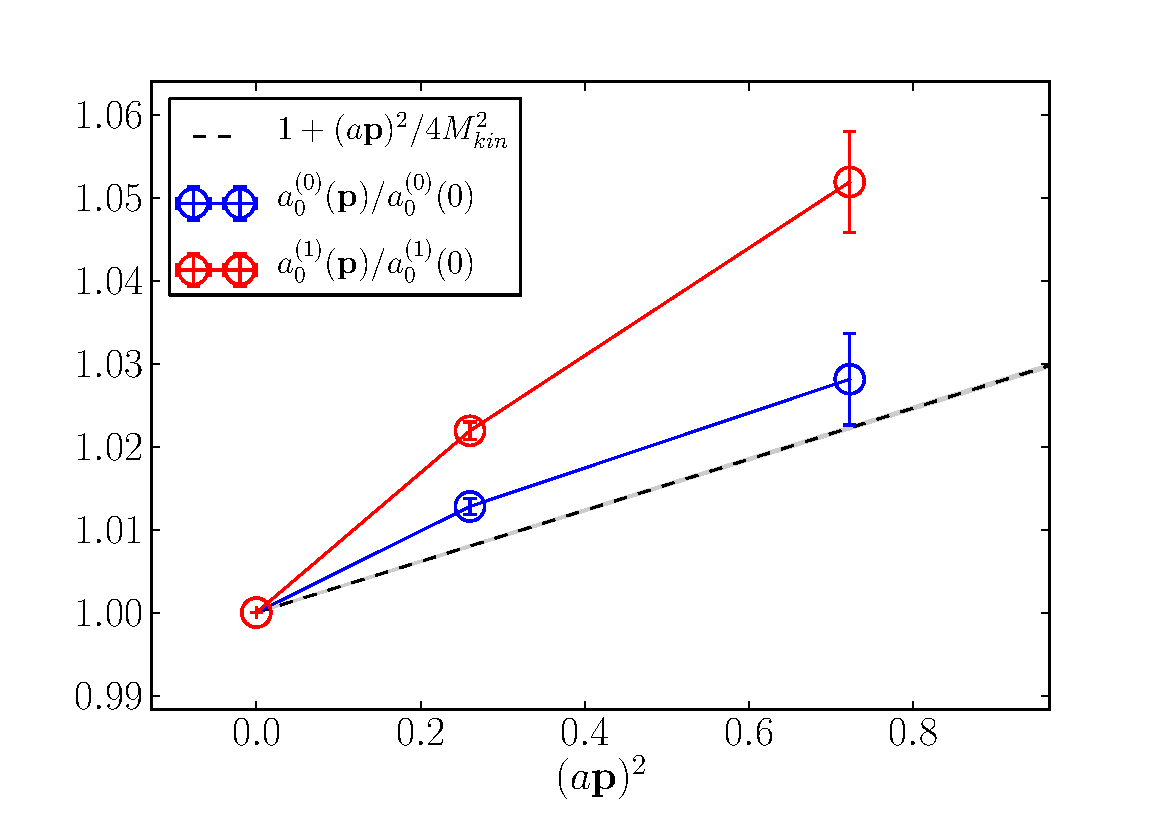
\includegraphics[width=0.85\textwidth]{images/nrqcd/relativistic_normalization_J0J1.pdf}
  \end{center}
  \caption{Decay amplitude ratios (colourful points) against the expected relativistic behaviour (grey dotted line and band). Adding the $A_{0,\text{lat}}^{(1)}$ piece of the current does not improve the relativistic behaviour of the ratio. \label{fig:relativisticnorm}}
\end{figure}

%% \subsubsection{Operator Matching}

%% In \cite{Morningstar:1997ep}, it is shown that this operator for the axial current by itself on the lattice is not totally sufficient to represent a continuum axial current. 
%% In this paper, the axial vector current with 1-loop corrections in continuum QCD (illustrated in figure 1, 2 and 3 in \cite{Morningstar:1997ep}) was computed using the on-shell mass and wave function renormalisation scheme in Feynman gauge. The light quark on-shell mass was approximated to zero, and the result was expanded in powers of the inverse heavy quark on-shell mass $1/M$.
%% \begin{align}
%% 	\nonumber
%% 	\langle q(p') | A_0 | h(p) \rangle_{\text{QCD}} = & \eta_1 [ \bar{u}_q(p') \gamma_5\gamma_0 u_h(p) ] + \eta_2 \left[ {p_0\over M} \bar{u}_h(p') \gamma_5 u_h(p) \right] \\
%% 	\nonumber
%% 	+ & \eta_3\left[ {p\cdot p'\over M^2} \bar{u}_q (p') \gamma_5\gamma_0 u_h(p)\right]
%% 	 + \eta_4\left[{p_0'\over M} \bar{u}_q(p') \gamma_5 u_h(p)\right] \\
%% 	 + & \mathcal{O}\left({1\over M^3}\right) \\ \nonumber \\
%% 	 \nonumber
%% 	 \eta_1 =  1 + &{\alpha_s\over 3\pi}\left[ 3\ln {M\over \lambda} - {11\over4} \right] \quad,\quad \eta_2 = {\alpha_s\over 3\pi} 2 \\
%% 	 \nonumber
%% 	 \eta_3 = {\alpha_s\over 3\pi} &\left[ 6\ln {M\over\lambda} - {8\pi\over 3}{M\over\lambda} + {1\over 2} \right] \quad,\quad \eta_4 = {\alpha_s\over 3\pi} \left[ -2 \ln {M\over \lambda} + {1\over 2} \right]
%% 	 \label{eq:continuum_axial}
%% \end{align}
%% $\lambda$ is the artificial Gluon mass (should cancel in obeservables), $|q(p')\rangle$ and $|h(p)\rangle$ are asymptotic light and heavy quark states respectively, and $u_{q,h}$ are the corresponding fermion wavefunctions. 

%% The dimensional requirements that $1/M$ must always come with a power of momenta turns this $1/M$ expansion into an expansion in velocity $v$, so is an NRQCD expansion. There are two expansions at play: $v$ and $\alpha_s$, one should avoid mixing them up.

%% In our lattice simulation the heavy quark obeys NRQCD so only has 2 components (there is no antiparticle without a relativistic dispersion relation). The particle and antiparticle fields in $h(x)$ can be decoupled using the Fouldy-Wouthuysen (FW) transformation \cite{Foldy:1949wa}, which is a canonical transformation, i.e. a change of variables of $h(x)$'s spinor degrees of freedom. Using the FW transformation, one can relate the $u_h$ to the wavefunction of a 2 component quark $U_h(p)$:
%% \begin{align}
%% 	u_h(p) = \exp\left(-{\underline{\gamma}\cdot{\textbf{p}}\over 2M}\right) \binom{U_h(p)}{0}
%% %	\label{eq:FW}
%% \end{align}
%% Using this to replace $u_h$ with $U_h$ in \eqref{eq:continuum_axial}, and inspecting the form of the leading order contributions, one can identify operators in the lattice theory that should be used to reproduce the continuum axial current $A_0$ \cite{Dowdall:2013tga}:
%% \begin{align}
%% 	&A_0 = (1+z_0 \alpha_s ) \left[ A_{0,\text{lat}}^{(0)} + (1 + z_1\alpha_s) A_{0,\text{lat}}^{(1)} + z_2\alpha_s A_{0,\text{lat}}^{(2)} \right]
%% 	\label{eq:current_corrections}
%% \\	&A_{0,\text{lat}}^{(0)} = \bar{c} \gamma_5 \gamma_0 b
%% 	\nonumber
%% \\	&A_{0,\text{lat}}^{(1)} = -{1\over2m_b} \bar{c} \gamma_5 \gamma_0 \underline{\gamma}\cdot\underline{\nabla} b
%% 	\nonumber
%% \\	&A_{0,\text{lat}}^{(2)} = -{1\over2m_b} \bar{c} \underline{\gamma}\cdot\underline{\overleftarrow{\nabla}} \gamma_5 \gamma_0  b.
%% 	\nonumber
%% \end{align}
%% $c$ and $b$ are the quark creation operators. The mass $M$ has been replaced with the bare $b$ mass $m_b$, since the on-shell mass only exists in perturbation theory so has no meaning in terms of the lattice. 
%% The coefficients $\{z_i\}$ can be obtained from matching terms between continuum and lattice perturbation theory.

%% The values $\{z\}$ are not yet known for the $bc$ current, but to give an idea of order or magnitude, in fig. \ref{fig:relativistic} uses values from the temporal axial current between light and $b$ quarks. Taken from \cite{Dowdall:2013tga}, these are $z_0=-0.007(2)$, $z_1=-0.031(4)$, $z_2=-0.325(4)$. $\alpha_s = 0.267$ is taken from set 7 of \cite{Colquhoun:2015oha}, obtained from running down of $\alpha_s^{\overline{MS}}(M_Z)$ down to scales of the simulation dictated by $a$.

%% $A_{0,\text{lat}}^{(0)}$ is the naive current operator used before (i.e with local smearing $\tilde{B}_c = A_{0,\text{lat}}^{(0)}$ in \eqref{eq:correlator}). 
%% To calculate the corrections, 
%% this was replaced with $A_{0,\text{lat}}^{(1,2)}$, and the calculation and fitting was repeated to extract $a_0$, this time coenciding with 
%% $\langle 0 | A_{0,\text{lat}}^{(1,2)} | B_c({\textbf{p}}) \rangle$. From these values one can build up a better estimation to the continuum current 
%% $\langle 0 | A_0 | B_c({\textbf{p}}) \rangle$. In fig. \ref{fig:relativistic} we gradually add corrections to see the effect each has, defining
%% \begin{align}
%%   \nonumber
%%   \label{eq:a_0corrections}
%%   &a_0^{(0)} = \langle 0 | (1+z_0 \alpha_s ) A_{0,\text{lat}}^{(0)} | B_c({\textbf{p}}) \rangle \\
%%   &a_0^{(1)} = \langle 0 | (1+z_0 \alpha_s ) \left[ A_{0,\text{lat}}^{(0)} + (1 + z_1\alpha_s) A_{0,\text{lat}}^{(1)} \right] | B_c({\textbf{p}}) \rangle \\
%%   \nonumber
%%   &a_0^{(2)} = \langle 0 | (1+z_0 \alpha_s ) \left[ A_{0,\text{lat}}^{(0)} + (1 + z_1\alpha_s) A_{0,\text{lat}}^{(1)} + z_2\alpha_s A_{0,\text{lat}}^{(2)} \right] | B_c({\textbf{p}}) \rangle \\
%%   \nonumber
%% \end{align}

%% \begin{table}
%% \begin{center}
%%  \begin{tabular}{||c c c c c c c c c||} 
%%  \hline
%%  set & $(a{\textbf{p}})^2$ & $a\delta E_0({\textbf{p}})$  & $aM_{B_c}$ & $a_0^{(0)}({\textbf{p}})/a_0^{(0)}(0)$ & $a_0^{(1)}({\textbf{p}})/a_0^{(1)}(0)$ 
%%  & $a_0^{(2)}({\textbf{p}})/a_0^{(2)}(0)$ \\ [0.5ex] 
%%  \hline\hline
%%  1 & 0.02891 & 0.00537(23) & 2.61(11) & 1.0036(19) & 1.0046(21) & 1.0045(21) \\ \hline
%%  2 & 0.26023 & 0.04580(24) & 2.838(27) & 1.0164(23) & 1.0253(26) & 1.0251(26) \\ \hline
%%  3 & 0.72287 & 0.12456(46) & 2.823(14) & 1.0371(46) & 1.0615(50) & 1.0608(51) \\ \hline
%%  4 & 1.04093 & 0.17772(86) & 2.840(15) & 1.053(10) & 1.088(11) & 1.086(11) \\ [1ex] 
%%  \hline
%% \end{tabular}
%% \end{center}
%% \caption{Results from fits with varying momenta. The third column gives the kinetic mass deduced from $\delta E({\textbf{p}})$ for each ${\textbf{p}}$. using \eqref{eq:kinetic_mass}\label{tab:from_fit}}
%% \end{table}

%% \subsubsection{$A_0^{(3)}$ contribution}

%% These current corrections are only to $\mathcal{O}({\textbf{p}}_b/m_b)$, but $\sqrt{E^r_{B_c}/M_{B_c}}$ has it's leading behaviour in $\mathcal{O}({\textbf{p}}^2/M_{B_c}^2)$. This implies one needs to carry on the expansion of current corrections further, to $\mathcal{O}(1/m_b^2)$. The dominant term at this order arises at tree level from the first term in \eqref{eq:continuum_axial}, and the second term in a $1/M$ expansion of \eqref{eq:FW}. The corresponding lattice operator is
%% \begin{align}
%% 	A^{(3)}_{0,\text{lat}} = {1\over 8m_b^2} \bar{c} \gamma_5\gamma_0 \underline{\nabla}^2 b. 
%% \end{align}
%% This was computed in a lattice calculation and combined with the lower orders to produce $a^{(3)}_0 = a_0^{(2)} + A^{(3)}_{0,\text{lat}}$. In this case we set $\alpha_s = 0$ to just focus on tree level. The results are shown on fig. \ref{fig:A3}.
%% \begin{figure}
%% \begin{center}
%%     \begin{tikzpicture}
%%         \begin{axis} [width=14cm,height=9cm,
%%             xmin=-0.1,xmax=0.9,ymin=0.99,ymax=1.09,
%%             xlabel = $(a{\textbf{p}})^2$,
%%             legend pos=north west]

%%             \addplot[color=green, dashed]{ sqrt( sqrt( x + 2.834*2.834 )/2.834) };
%%             \addlegendentry{$\sqrt{E_{B_c}/M_{B_c}}$}

%%             \addplot+[color=blue, mark=*,
%%                     error bars/.cd,x dir=both, x explicit,  y dir=both, y explicit]
%%                 coordinates {
%%                 		(  0.0 ,  1.0  ) +- ( 0.0,  1.33226762955e-19  )
%% 		  	(  0.0289148446127 ,  1.00549267643  ) +- ( 0.0,  0.00176452228481  )
%% 			(  0.260233601514 ,  1.01836440302  ) +- ( 0.0,  0.00222088535291  )
%% 			(  0.722871115317 ,  1.0390590324  ) +- ( 0.0,  0.00452197676768  )
%%             };
%%             \addlegendentry{$a_0^{(0)}({\textbf{p}})/a_0^{(0)}(0)$}

%%             \addplot+[color=red, mark=*,
%%                     error bars/.cd,x dir=both, x explicit,  y dir=both, y explicit]
%%                 coordinates {
%%                 		(  0.0 ,  1.0  ) +- ( 0.0,  0.0  )
%%           	        (  0.0289148446127 ,  1.00663334793  ) +- ( 0.0,  0.00194538583335  )
%% 			(  0.260233601514 ,  1.02734203998  ) +- ( 0.0,  0.00244820981549  )
%% 			(  0.722871115317 ,  1.06347584999  ) +- ( 0.0,  0.00497690081001  )
%%             };
%%             \addlegendentry{$a_0^{(1)}({\textbf{p}})/a_0^{(1)}(0)$}
            
%%             \addplot+[color=orange, mark=*,
%%                     error bars/.cd,x dir=both, x explicit,  y dir=both, y explicit]
%%                 coordinates {
%%                 		(  0.0 ,  1.0  ) +- ( 0.0,  0.0  )
%% 			(  0.260233601514 ,  1.0211157939  ) +- ( 0.0,  0.00302333986783  )
%% 			(  0.722871115317 ,  1.05858288737  ) +- ( 0.0,  0.00568371480017  )
%%             };
%%             \addlegendentry{$a_0^{(3)}({\textbf{p}})/a_0^{(3)}(0)$}

%%         \end{axis}
%%     \end{tikzpicture}
%% \end{center}
%% \caption{Relativistic Normalisation of 1-loop corrected Axial Current. $a_0^{(n)}$ are defined in \eqref{eq:a_0corrections}. (tree level) }
%% \label{fig:A3}
%% \end{figure}
%% As a sanity check for the $A^{(3)}$ calculation, fig. \ref{fig:A3A2} shows the ratio $A^{(3)}_{0,\text{lat}}({\textbf{p}})/A^{(2,1)}_{0,\text{lat}}({\textbf{p}})$. Since $A^{(3)} = \mathcal{O}({\textbf{p}}^2)$ and $A^{(1)} = \mathcal{O}({\textbf{p}})$, we expect such a ratio to be proportional to $|{\textbf{p}}|$ (see fig. \ref{fig:A3A1}). {\color{red}{The $A^{(3)}/A^{(2)}$ line isn't straight...}}

%% %==========
%% \begin{figure}
%% \begin{center}
%%     \begin{tikzpicture}
%%         \begin{axis} [width=14cm,height=9cm,
%%             xlabel = $a|{\textbf{p}}|$,
%%             legend pos=north west]

%%             \addplot+[color=red, mark=*,
%%                     error bars/.cd,x dir=both, x explicit,  y dir=both, y explicit]
%%                 coordinates {
%%                		(  0.0 ,  0.168061897514  ) +- ( 0.0,  0.00761364082979  )
%% 			(  0.510130965061 ,  0.255812358549  ) +- ( 0.0,  0.0171547894616  )
%% 			(  0.850218275102 ,  0.291882276843  ) +- ( 0.0,  0.0323767757253  )
                    
%%             };
%% \addlegendentry{$A^{(3)}_{0,\text{lat}}({\textbf{p}})/A^{(1)}_{0,\text{lat}}({\textbf{p}})$}

%%         \end{axis}
%%     \end{tikzpicture}
%% \end{center}
%% \label{fig:A3A1}
%% \caption{Ratio of third current correction to first.}
%% \end{figure} 

\section{$B_{(s)}\to D_{(s)}l\nu$ form factors}
\label{sec:BD_BsDs_nrqcd}

We attempted a calculation of the $B\to Dl\nu$ and $B_{s}\to D_{s}l\nu$ form factors, $f_{0,+}(q^2)$ and $f^s_{0,+}(q^2)$, using the 2+1+1 MILC ensembles, HISQ $l$,$s$ and $c$ valence quarks, and an NRQCD valence $b$ quark. This study was similar to previous studies of $B\to Dl\nu$ form factors \cite{Na:2015kha} and $B_s\to D_sl\nu$ form factors \cite{Monahan:2017uby}. The main difference between this and the previous studies was that they used older MILC ensembles that do not take the charm into account in the sea.

This study was not completed on account of two major problems:
\begin{itemize}
  \item
    The $\alpha_s{\textbf{p}}/m_b$ terms in the vector NRQCD-HISQ current that we must ignore due to the lack of perturbative normalizations, $V_{k}^{(2)}$ and $V_{k}^{(4)}$, turned out to be significant in magnitude.
  \item
    On one ensemble in the $B_s\to D_s l\nu$ case, there was an anomalous result for the vector current matrix element extracted from the correlator fits.
\end{itemize}
We give an outline of the calculation here for completeness, but the crucial findings of this section are these two issues.

\subsection{Calculation Details}

\begin{table}[t!]
\hspace{-40pt}
 \begin{tabular}{c c c c c c c c c c c}
 \hline
 Set & handle & $am_{s0}$ & $am_{c0}$ & $am_{b0}$ & $u_0$ & $c_{1,6}$ & $c_5$ & $c_4$ & $\{T\}$ & $a_{\text{sm}}/a$ \\ [0.5ex] 
 \hline
 0 & {\textbf{very coarse}} & 0.0705 & 0.826 & 3.297 & 0.8195 & 1.36 & 1.21 & 1.22 & 8, 11, 14 & 0, 2.0, 4.0 \\ [1ex]
 1 & {\textbf{coarse}} & 0.0541 & 0.645 & 2.66 & 0.8340 & 1.31 & 1.16 & 1.20 & 9, 12, 15 & 0, 2.0, 4.0 \\ [1ex]
 2 & {\textbf{fine}} & 0.0376 & 0.450 & 1.91 & 0.8525 &  1.21 & 1.12 & 1.16 & 14, 19, 24 & 0, 3.425, 6.85 \\ [1ex]
 \hline
\end{tabular}
 \caption{Parameters used in our calculation. $am_{s0}$ and $am_{c0}$ are the bare masses of the strange, charm valence quarks, tuned in \cite{PhysRevD.91.054508}, $am_{b0}$ is the bare mass of the valence bottom quark, tuned in \cite{Dowdall:2011wh} $u_0$ is the 'tadpole improvement parameter' as used in \cite{Dowdall:2011wh}. $\{c_i\}$ are the coefficients for the kinetic and chromomagnetic terms in the NRQCD action (eq. \eqref{eq:nrqcd_dH}) \cite{Hammant:2013sca}. $\{T\}$ is the set of temporal seperations between source ($B_s$ creation operator) and sink ($D_s$ anihilation operator). $a_{\text{sm}}$ are the radii of the exponential smearing function applied to the $B_{(s)}$ and $D_{(s)}$ creation operators.
   \label{tab:quarkmasses}}
\end{table}

We generated correlation functions on three MILC ensembles, sets 0, 1 and 2 in table \ref{tab:ensembles}. When using the NRQCD action, we are limited to the coarser end of the spectrum of ensembles. This is because in the $a\to 0$ limit subleading terms in $\delta H$ (eq. \eqref{eq:nrqcd_dH}) and $J^{(n>0)}_{\mu}$ (eq. \eqref{eq:nrqcd-hisq-current}) diverge, since in lattice units the $1/m_b$ factors become $1/am_b$, resulting negative powers of the lattice spacing. However, NRQCD discretisation effects are small relative to other discretizations due to the lack of the $b$ rest mass, so we can afford to use coarser lattices. Also, obviously, using coarse lattices means the project is computationally inexpensive. The bare parameters used to generate the correlation functions are shown in table \ref{tab:quarkmasses}.

We generate 2-point correlation functions for $B_{(s)}$ and $D_{(s)}$ mesons, and 3-point correlators between $B_{(s)}$ and $D_{(s)}$ interpolating operators with $V^{(n)}_{\mu}$ currents inserted for all $\mu$ and $n=0,1,2$($\mu=0$) and $n=0,1,2,3,4$($\mu=1,2,3$). For the $B_{(s)}$ operator we use smearings like those introduced in eq. \eqref{eq:smearings}, smearing radii $a_{\text{sm}}$ are given in table \ref{tab:quarkmasses}.

The $B_{(s)}$ 2-point correlators, $C_{B_{(s)}}^{\alpha\beta}(t)$ are generated using eq. \eqref{eq:nrqcd-hisq-2pt}, with the charm propagator replaced with a strange or light propagator, and $\mathcal{O}_{m} = \gamma_0\gamma_5$. We generate $D_{(s)}$ 2-point correlators at a number of spacial momenta $\{{\textbf{p}}\}$, generated by
\begin{align}
  C_{D_{(s)}}^{\alpha\beta}({\textbf{p}},t) = \sum_{{\textbf{x}},{\textbf{x}}'}\sum_{{\textbf{y}},{\textbf{y}}'} \phi^{\alpha}({\textbf{x}}-{\textbf{x}}')\phi^{\beta}({\textbf{y}}-{\textbf{y}}') \left\langle \text{Tr}_c[g_c^{\theta_{\textbf{p}}}(x,y) g^{\dagger}_{l(s)}(x',y') ]\right\rangle,
\end{align}
where $\phi^{\alpha}({\textbf{x}})$ are the smearing functions defined in eq. \eqref{eq:smearings}, $g_{l(s)}$ are light or strange staggered propagators, and $g_c^{\theta_{\textbf{p}}}$ is a charm staggered propagator with momentum twist $\theta_{\textbf{p}}$. Tr$_c$ is over color.

We generate 3-point correlators for each individual piece of the NRQCD-HISQ current, and each {\textbf{p}}, using
\begin{align}
  C_{V_{\mu}^{(n)}}^{\alpha\beta} ({\textbf{p}},t,T) = \sum_{\textbf{x},\textbf{y},\textbf{z}} \left\langle \text{Tr}_c\left( g_c^{\theta_{\textbf{p}}}(x,y) g_{l(s)}^{\dagger}(x,z) \text{Tr}_s\left[ \gamma_0 \gamma_x\gamma_y \mathcal{O}_{n,\mu}G_b(y,z) \gamma_z \right] \right) \right\rangle.
\end{align}
$\mathcal{O}_{n,\mu}$ are defined by $J_{\mu}^{(n)} = \bar{\psi}_c \mathcal{O}_{n,\mu} \Psi_b$, where $J_{\mu}^{(n)}$ are the NRQCD-HISQ vector currents given in Eq. \eqref{eq:nrqcd-hisq-current}.

The list of twists we used on each ensemble is given in table \ref{tab:nrqcd_twists}. Due to the signal/noise degradation of the $D_{(s)}$ correlators as one adds more spacial momentum, our lattice data was limited to the high $q^2$ region. One motivation for this study was to test how far down the $q^2$ range we could reach with lattice data before the noise in the correlators made the data useless.

\begin{table}[htb!]
  \vspace{10pt}
  \hspace{-15pt}
 \begin{tabular}{c c c c c}
 \hline
 & Set & $\theta$ & $|a{\textbf{p}}|$ & $q^2$[GeV$^2$] \\ [0.5ex] 
 \hline
 $B\to D$ & 0 & 0, 0.74, 1.47, 2.20, 2.94 & 0, 0.25, 0.5, 0.75, 1.00 & 11.8, 11.6, 10.8, 9.4, 7.3 \\ [1ex]
 & 1 & 0, 1.58, 2.24, 4.53 & 0, 0.36, 0.51, 1.02 & 11.8, 10.8, 9.9, 5.0  \\ [1ex]
 & 2 & 0, 1.76, 2.64 & 0, 0.30, 0.49 & 11.8, 10.7, 9.3 \\ [1ex]
 \hline
 $B_s\to D_s$ & 0 & 0, 0.74, 1.47, 2.20, 2.94 & 0, 0.25, 0.5, 0.75, 1.03 & 11.8, 11.6, 10.9, 9.5, 7.6 \\ [1ex]
 & 1 & 0, 1.10, 2.20, 3.31, 4.41 & 0, 0.25, 0.50, 0.75, 1.00 & 11.8, 11.3, 10.1, 8.1, 5.7 \\ [1ex]
 & 2 & 0 & 0 & 11.8\\  [1ex]
 \hline
\end{tabular}
 \caption{Twists given to the charm propagator on each ensemble. \label{tab:nrqcd_twists} }
\end{table}

\subsection{Correlator Fits}

We extract current matrix elements from the generated correlation functions, via simultaneous Bayesian fits as described in Sec. \ref{sec:correlator_fits}. For the set of 2-point correlators we use \eqref{eq:2ptfit_wsmears}, and 3-point correlators are fit to
\begin{align}
  \nonumber
  C^{\alpha\beta}_{3}(t,T)|_{\text{fit}} =& \sum_{j,k=0}^{N_{\text{exp}},N_{\text{exp}}} \Big(\, a^{M}_j J^{nn}_{jk} a^{M'}_k f(E^{H_s},t) f(E^{M'}_n,T-t)
  \\ \nonumber
  &+a^{M,o}_{\alpha,j} J^{on}_{jk} a_{\beta,k}^{M'} (-1)^t f(E^{M,o}_n,t) f(E^{M'},T-t)
  \\ \nonumber
  &+a_{\alpha,j}^{M} J^{no}_{jk} a_{\beta,k}^{M',o} (-1)^{T-t} f(E^{M},t) f(E^{M'^*,o}_n,T-t)
  \\
  &+a_{\alpha,j}^{M,o} J^{oo}_{jk} a_{\beta,k}^{M',o} (-1)^T f(E^{M,o}_n,t) f(E^{M',o},T-t) \,\Big).
  \label{eq:3ptcorrelator_real}
\end{align}
We set $N_{\text{exp}}=5$ is each fit. We perform a single simultanious fit containing each correlator computed for each ensemble.

We set gaussian priors for the parameters $J_{jk}$, and log-normal priors for all other parameters. Using log-normal distributions forbids energies $E_n^M$ and amplitudes $a_n^M$ from moving arbitrarily close to zero, improving the stability of the fit.

Priors for the ground state energies and amplitudes (oscillating and non-oscillating) are set via an empirical Bayes approach, plots of effective masses and amplitudes are inspected to find reasonable central values of priors (see Sec. \ref{sec:BsDsstar_fits} for definitions of effective masses and amplitudes). A generic variance of 10\% of the central value is given in all cases. The typical precision of fit results for these parameters is of order 0.1\%, much more precise than their priors. All 3-point transition parameters $J_{jk}$ are given priors of $0\pm 1$.

We typically set $t_{\text{cut}}=3$ for 2- and 3-point correlators in the fit on the fine ensemble (set 2) and $t_{\text{cut}}=2$ on very coarse and coarse (sets 0 and 1). For some specific correlators, a larger $t_{\text{cut}}$ is necessary to acheive a good fit ($\chi^2/N_{\text{dof}} < 1$), these higher $t_{\text{cut}}$ values are always in the range $t_{\text{cut}}\in[2,8]$. An svd-cut is applied in each fit, with a specific choice of cut determined according to what acheives a good fit. The svd-cut is typically of the order $10^{-3}$.

The current matrix element we require to find $h_{A_1}^s(1)$ is given by
\begin{align}
  \langle D_s | V_{\mu}^{(m)} | B_s \rangle |_{\text{lat}} = 2 \sqrt{M_{B_s}E_{D_s}} J^{nn}_{00}.
  \label{eq:currentfit}
\end{align}

\subsection{Form Factors}

We construct 'continuum' vector currents $\langle D_{(s)}| V_{\mu} | B_{(s)} \rangle \equiv \langle V_{\mu} \rangle$ from the lattice expectation values $\langle D_s | V_{\mu}^{(n)} | B_s \rangle |_{\text{lat}}$ according to Eq. \eqref{eq:nrqcd-hisq-current-truncate}, i.e. only including the first two current pieces $V^{(0)}_{\mu}$ and $V^{(1)}_{\mu}$. We also compute $V^{(2)}_{0}$ and $V^{(2,3,4)}_k$ to assess their size and the validity of ignoring them, this is adressed in Sec. \ref{sec:largesubleadingcurrents}.

We take the average over the spacial currents, resulting in two distinct current matrix elements $\langle V_0 \rangle$ and $\langle V_k \rangle$. Then, from the definition of pseudoscalar-pseudoscalar form factors (Eq. \eqref{eq:formfactors_experimental}), we find (defining $M_{B_{(s)}}\equiv M$, $M_{D_{(s)}}\equiv m$, $E_{D_{(s)}}\equiv E$, and ${\textbf{p}}_{D_{(s)}} \equiv {\textbf{p}}$)
\begin{align}
  \langle V_0 \rangle &= f^{(s)}_+(q^2) \left[ M + E - {M^2-m^2\over q^2}(M-E) \right] + f^{(s)}_0(q^2) {M^2-m^2\over q^2}(M-E), \\
  \langle V_k \rangle &= {|{\textbf{p}}|\over \sqrt{3}} \left[ f^{(s)}_+(q^2) \left( 1 + {M^2-m^2\over q^2} \right) - f^{(s)}_0(q^2) {M^2-m^2\over q^2} \right].
\end{align}
By inverting these relations we deduce $f^{(s)}_{0,+}(q^2)$ from $\langle V_0 \rangle$,$\langle V_k \rangle$ at the lattice spacings of each ensemble.

We aim then to extrapolate these form factors to $a=0$ and to all $q^2$. We did not obtain any lattice data at smaller light quark masses so cannot extrapolate to the physical light mass. In the $B_s\to D_sl\nu$ case, the size of such an effect is small (see chapters \ref{chap:BsDsstar} and \ref{chap:BsDs}). In the $B\to Dl\nu$ case, however, this could result in considerable uncontrolled systematic errors.

We parameterise the functional form of $f^{(s)}_{0,+}(q^2)$ using the BGL parameterization \cite{PhysRevD.79.013008}. This involves first defining the map
\begin{align}
	z(q^2) = {\sqrt{t_+ - q^2} - \sqrt{t_+ - t_0} \over \sqrt{t_+ - q^2} + \sqrt{t_+ - t_0} }.
\end{align}
where we take $t_0 = t_+( 1 - \sqrt{1 - t_-/t_+})$, and $t_{\pm} = (M_{B_{(s)}} \pm M_{D_{(s)}})^2$. $z(q^2)$ has a very small magnitude throughout the entire $q^2$ range, in our case $|z| < 0.032 \,\,\forall\,q^2$. It can be shown that $f_{0,+}^{(s)}(q^2)$ is analytic in the unit disc of the $z-$plane (see e.g. \cite{Hill:2006ub}). $f^{(s)}_{+,0}(q^2)$ can be expressed as a series expansion in $z$:
\begin{align}
	f_{0,+}(q^2) = {1\over P_{0,+}(q^2)} \sum_k a^{0,+}_k z(q^2)^k.
	\label{eq:zexpansion}
\end{align}
we truncate this at $z^2$, adding further terms have no effect on the fit. The factors $P(q^2)$ are defined by
\begin{align}
	P_{0,+}(q^2) = \left( 1 - {q^2\over M_{0,+}^2}\right).
\end{align}
These are required due to subthreshold poles in the crossed channel of $\langle D_{(s)} | V_{\mu} | B_{(s)} \rangle$, which in our case is a $W$ decay into a $B_c$ meson. The pole is located where the $W$ has the correct momentum $q^2$ to create the $B_c$, hence at $q^2=M_{B_c}$. This is not within the $q^2$ range, but can create curvature in $f_{0,+}$ that can confound the expansion in $z$. $P_{0,+}$ effectively removes this pole from the $z$ expansion.

The discretisation effects in our form factors are controlled for by modifying \eqref{eq:zexpansion};
\begin{align}
	a^{0,+}_n \to a^{0,+}_n \times ( 1 + b^{0,+}_n (am_c)^2 ),
\end{align}
where $b^{0,+}_n$ are new fit parameters, and $m_c$ is the charm mass. $am_c\to0$ in the continuum limit, and, since the charm mass is the largest scale involved in our calculation, it serves as a good order parameter for discretization effects. 

\subsection{Results}

%% \begin{figure}
%% \centering
%% \begin{subfigure}{.55\textwidth}
%%   \centering
%%   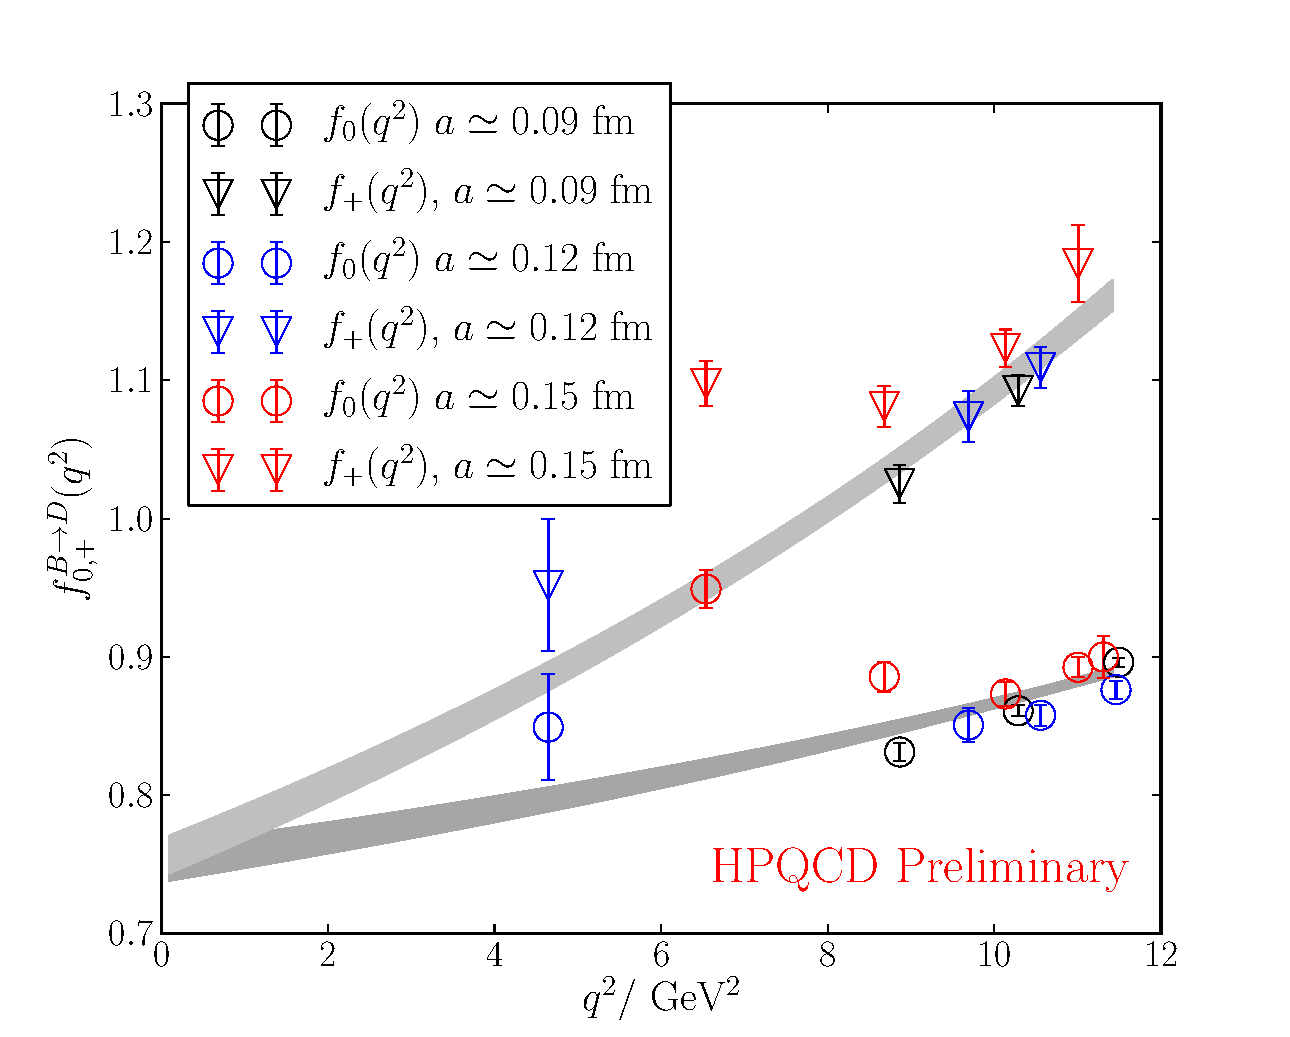
\includegraphics[width=1.0\linewidth]{images/NRQCD/BD_apr18.pdf}
%%   \label{fig:sub1}
%% \end{subfigure}%
%% \begin{subfigure}{.55\textwidth}
%%   \centering
%%   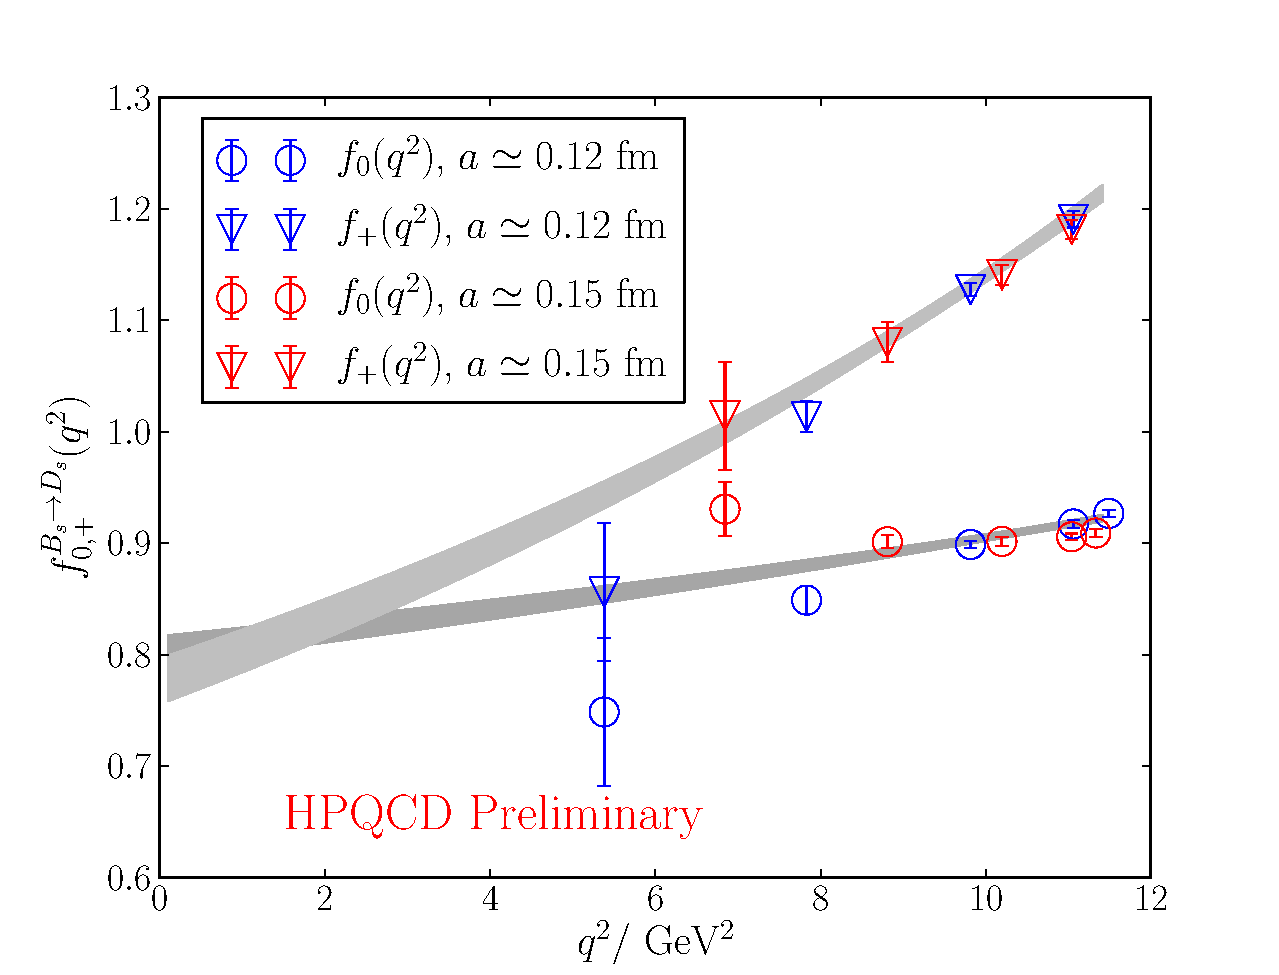
\includegraphics[width=1.0\linewidth]{images/NRQCD/BsDs_apr18.pdf}
%%   \label{fig:sub2}
%% \end{subfigure}
%% \caption{Left: $B\to D l\nu$ form factors from the NRQCD calculation. Right: $B_{(s)}\to D_{(s)} l\nu$ form factors using an identical approach. Errors are statistical. The bands give a kinematic extrapolation to all $q^2$, see second year report. The statistical errors grow as $q^2$ decreases due to Parisi-Lepage scaling (sec.9.3.2 of \cite{DeGrand:2006zz}).}
%% \label{fig:nrqcd}
%% \end{figure}

The extrapolation of our lattice data to all $q^2$ and $a=0$ is illustrated in figures \ref{fig:BD_formfactors} and \ref{fig:BsDs_formfactors}. As can be seen here, statistical errors in the lattice data increase exponentially with momentum twist (as $q^2$ decreases). Besides this, the very coarse data suffers from large discretization effects as the twist is increased, pushing the results upwards.

\begin{figure}[htb!]
  \begin{center}
    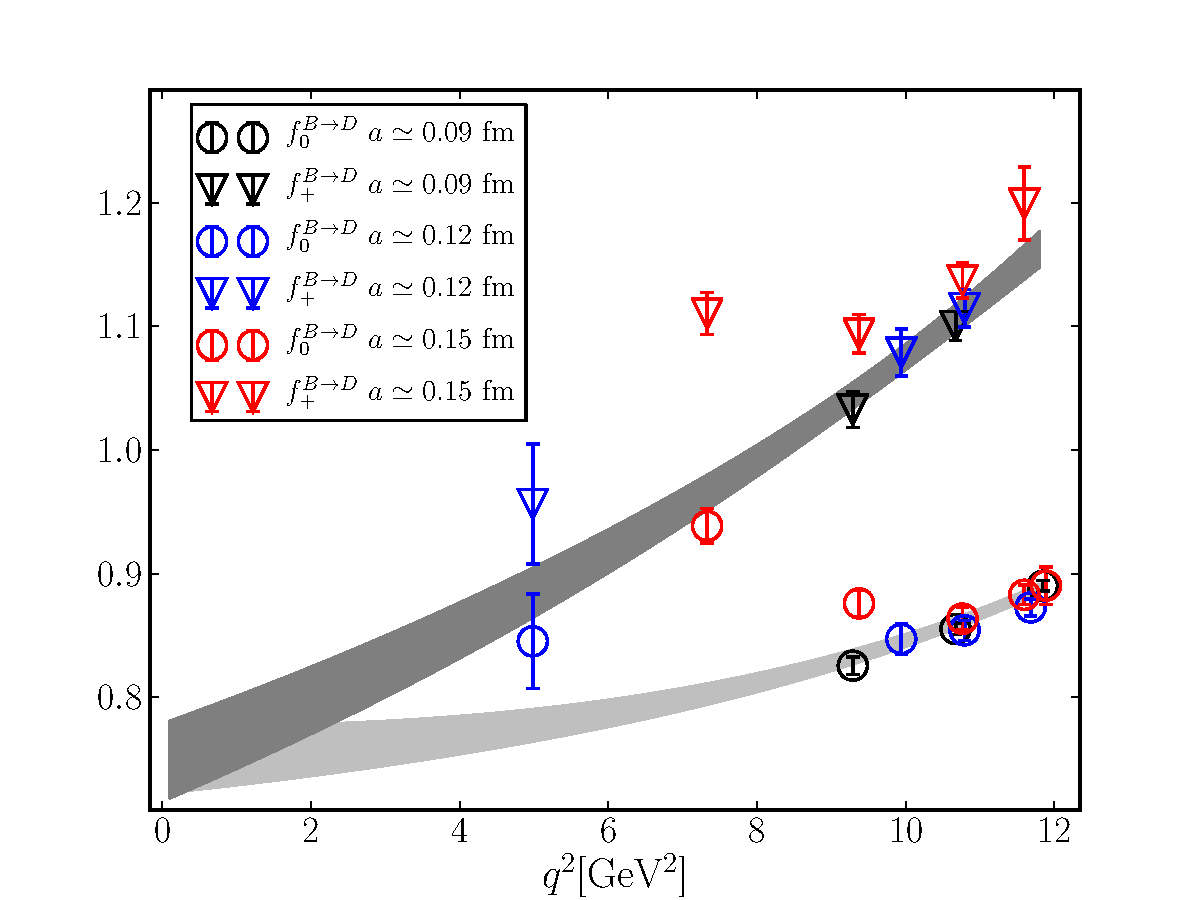
\includegraphics[width=0.85\textwidth]{images/nrqcd/BD_formfactors.pdf}
  \end{center}
  \caption{$B\to Dl\nu$ form factors. The coloured points show lattice data, each color represents an ensemble. The grey band represents the continuum and kinematically extrapolated result. \label{fig:BD_formfactors}}
\end{figure}

\begin{figure}[htb!]
  \begin{center}
    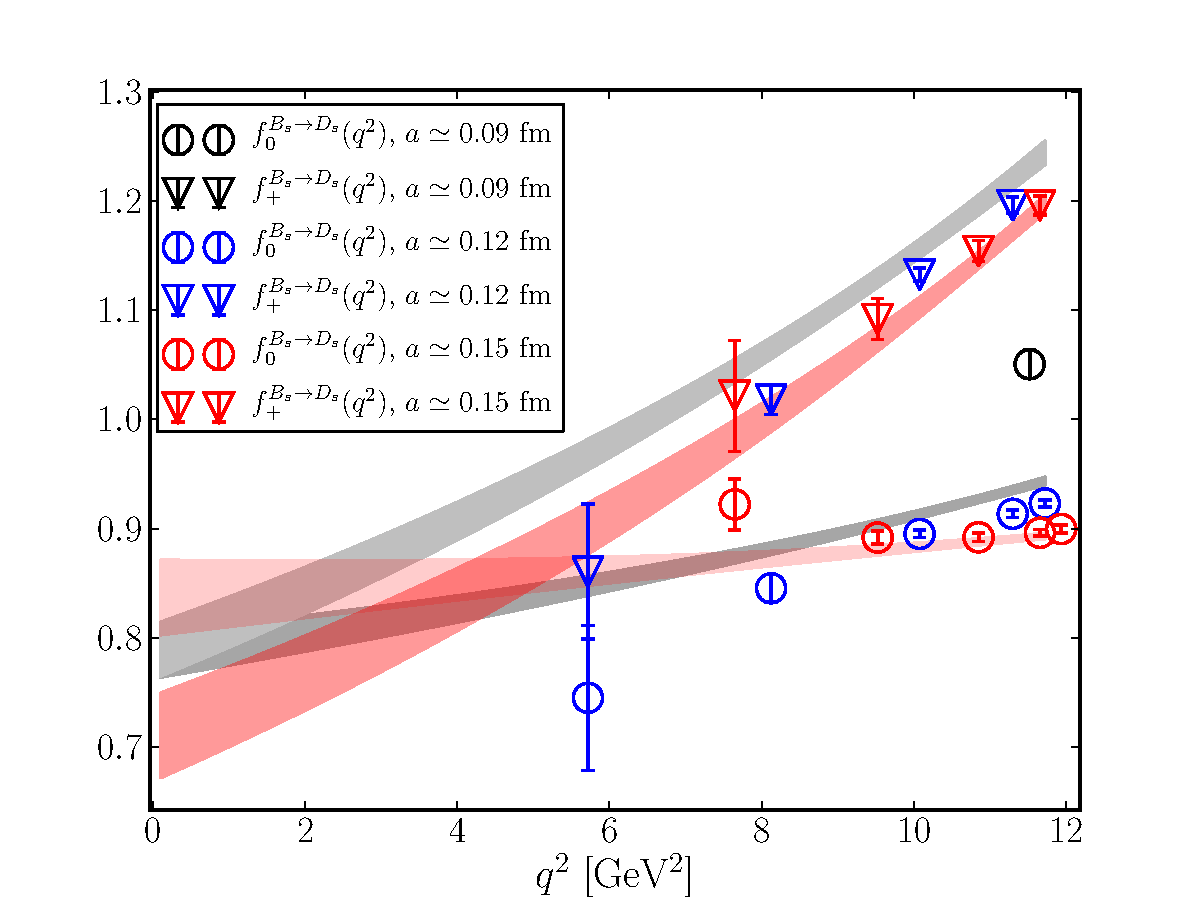
\includegraphics[width=0.85\textwidth]{images/nrqcd/BsDs_formfactors.pdf}
  \end{center}
  \caption{$B_s\to D_sl\nu$ form factors. The coloured points show lattice data, each color represents an ensemble. The grey band represents the continuum and kinematically extrapolated result. \label{fig:BsDs_formfactors}}
\end{figure}

We now go on to discuss the two issues which lead us to abandon this project.

\subsubsection{Anomalous Results}

In the $B_s\to D_s l\nu$ case we did not include lattice results from the fine ensemble in the $q^2$ and $a\to 0$ extrapolation. This is because the lattice results for $f_0^s(q^2)$ on this ensemble are clearly wrong. We have {\textit{a priori}} knowledge of what, for example, the ballpark of $f_0^s(q^2_{\text{max}})$ should be from a couple of sources:
\begin{itemize}
\item
The result should not vary much more than $\mathcal{O}(a^2)$ (where $a$ is the lattice spacing) from the same result on other ensembles.
\item
  The result should not vary much more than $\mathcal{O}(am_s - am_l)$ from the same number on the same ensemble for the $B\to D$ calculation (Chiral symmetry).
\end{itemize}
However, we find the fits to $q^2_{\text{max}}$ data on the fine ensemble produce a result for $J^{nn}_{00}$ that is much larger than expected. This is accompanied by the fits being very unstable, varying by a number of sigmas when different combinations of data are included, and different hyperparameters (svd-cut, $t_{\text{cut}}$, etc) are included. A number of tests have been carried out to find out exactly what is causing this issue, but no compelling evidence has emerged for any explanation. Fig. \ref{fig:BsDs_f0q2max} illustrates the situation.

It is worth keeping in mind that NRQCD results have no continuum limit since the action and the currents are truncated sums of inverse masses in lattice units, therefore the truncation error grows like $a^{-n}$ as $a\to 0$. What we are seeing here may be the result of large $1/(am_b)^2$ corrections to the NRQCD-HISQ current being ignored.

\begin{figure}[htb!]
  \vspace{-20pt}
  \begin{center}
    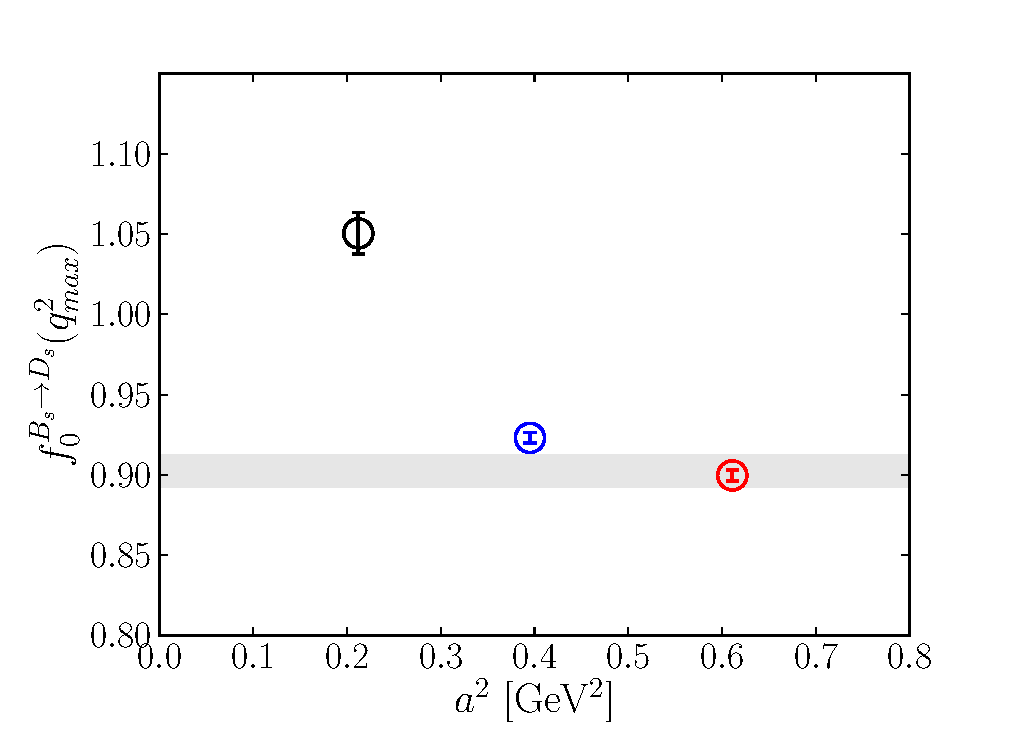
\includegraphics[width=0.75\textwidth]{images/nrqcd/BsDs_f0q2max.pdf}
  \end{center}
  \caption{Lattice results for $f_0^s(q^2_{\text{max}})$ against $a^2$. The grey band shows the result for $f_0^s(q^2_{\text{max}})$ computed in chapter \ref{chap:BsDs} using the Heavy-HISQ approach for comparison. Clearly the result on the fine ensemble (the black point), and possibly on the coarse ensemble (the blue point), contain large unknown systematic errors. \label{fig:BsDs_f0q2max}}

\end{figure}

\subsubsection{Large Subleading Currents}
\label{sec:largesubleadingcurrents}

Another problem that has uncovered itself in the NRQCD calculation is large subleading currents. Namely, the pieces $V^{(2,4)}_k$ of the spatial vector current. We determined these currents as part of the calculation in order to assess if they are suitably small such that they can be ignored. These turned out to have a magnitude $\sim 35\%$ of the leading order.

\begin{figure}[htb!]
  \begin{center}
    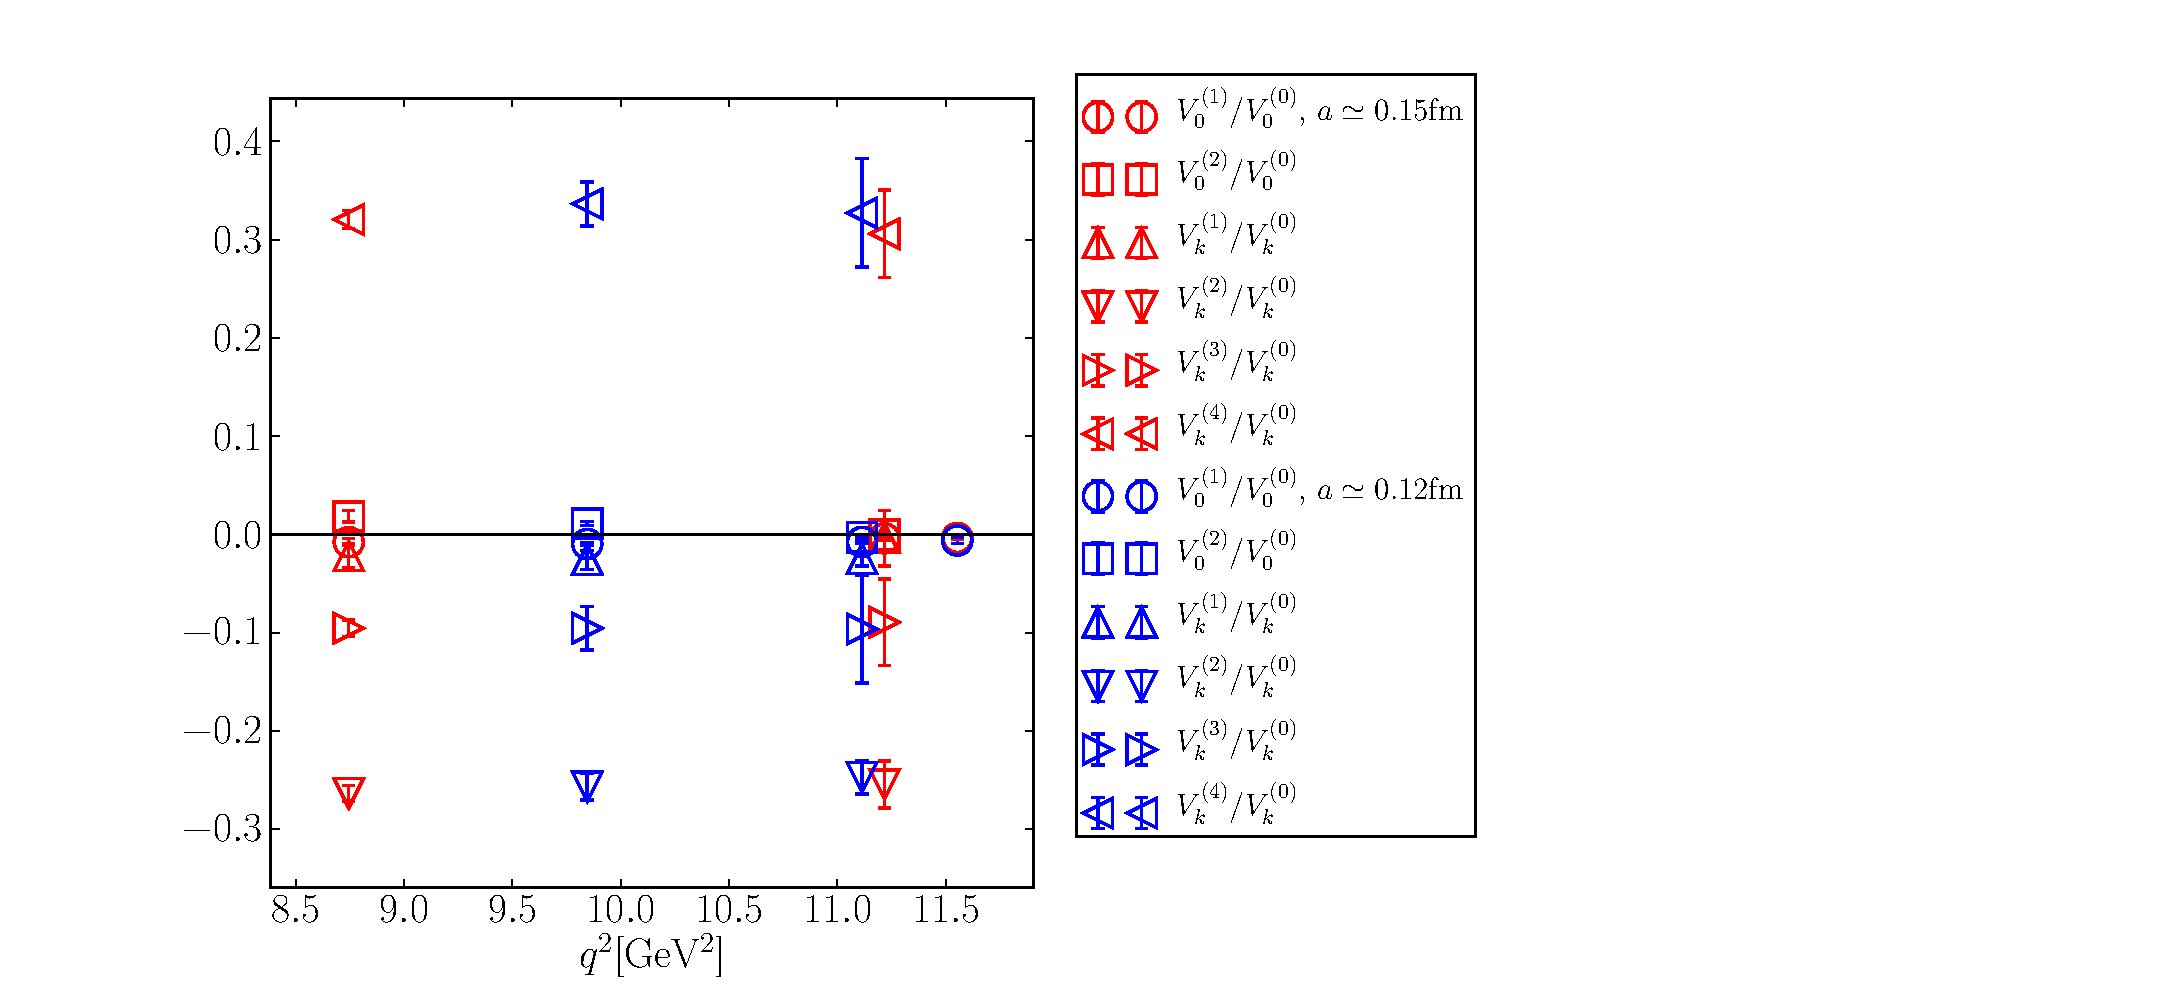
\includegraphics[width=1.2\textwidth]{images/nrqcd/BsDs_currentratios.pdf}
  \end{center}
  \caption{Ratios of (matrix elements of) the subleading NRQCD-HISQ currents $V_{\mu}^{(n>0)}$ to the leading order current $V_{\mu}^{(0)}$, in the $B_s\to D_s$ case. \label{eq:currentratios}}
\end{figure}

In Fig. \ref{eq:currentratios}, we show the ratios of (matrix elements of) NRQCD-HISQ currents in the $B_s\to D_s$ case. All ratios are between the subleading currents $V_{\mu}^{(n>0)}$ and the leading order current $V_{\mu}^{(0)}$, in order to show the size of the subleading currents relative to the leading order. $V^{(1)}_{\mu}$ is included in our result so we do not need to worry about its size. $V_0^{(2)}$ and $V_k^{(3)}$ are $\lessapprox 10\%$ of the leading order, given that these also receive $\order{\alpha_s}$ suppression, their negligence is relatively harmless.

$V_k^{(2,4)}$, however, have considerable magnitude. Neglecting them implies a naive systematic error of $\order{ 35\% \times \alpha_s } \sim 8\%$. This would prevent any results from our calculation from being anywhere near competitive. These two currents are of order $\alpha_s{\textbf{p}}/m_b$, so their magnitude would likely only increase as we move towards $q^2=0$.

Since the problematic current pieces are exclusively part of the spacial vector current, we could remove this problem if we did not rely on the spacial vector current for extracting the form factors. The next section shows our attempt at such an alternative approach.

\subsection{Form factors from $V_0$ and $S$ in $B_{(s)}\to D_{(s)}$}
\label{sec:fplus_divergence}

Instead of using $\langle V_0 \rangle$ and $\langle V_k \rangle$ to extract $f^{(s)}_{0,+}(q^2)$, one could in principle instead use the combination $\langle V_0 \rangle$ and $\langle S \rangle$, where $S$ is the scalar $b\to c$ density. In terms of NRQCD-HISQ currents, $S$ can be written as
\begin{align}
  S &= (1+z_0^S\alpha_s)V^{(0)}_0 - (1+z_1^S\alpha_s)V^{(1)}_0 + z_2^S\alpha_sV_0^{(2)}\\ \nonumber &\quad\quad + \mathcal{O}(\alpha_s^2,\, (\Lambda_{\text{QCD}}/m_b)^2,\, ({\textbf{p}}/m_b)^2 ), \\
  &= (1+z_0^S\alpha_s)( V^{(0)}_0 - V_0^{(1)} )  \\ \nonumber &\quad + \mathcal{O}(\alpha_s^2,\, (\Lambda_{\text{QCD}}/m_b)^2,\, ({\textbf{p}}/m_b)^2,\,\, \alpha_s \Lambda_{\text{QCD}} / m_b,\, \alpha_s {\textbf{p}}/m_b, ).
\end{align}
$z_0^S$ can be derived from $z_0^{V_{\mu}}$. Hence we infact already have numerical results for matrix elements of the scalar current, via the vector current pieces $V^{(0,1)}_0$. The scalar and temporal vector currents are related via the parially conserved vector current (PCVC) relation -
\begin{align}
  &(M_{B_{(s)}}-E_{D_{(s)}})\langle V_0 \rangle = \delta m \langle S \rangle,
\end{align}
where $\delta m \equiv (m_b-m_c)$. Using this one can relate the scalar current to the form factors, resulting in a new way to extract form factors via $\langle V_0 \rangle$ and $\langle S \rangle$:
\begin{align}
  f_0^{(s)}(q^2) &= {\delta m\over M_{B_{(s)}}^2 - M_{D_{(s)}}^2 } \langle S \rangle, \\
  f_+^{(s)}(q^2) &= {1\over 2M_{B_{(s)}}} { (M_{B_{(s)}}-E_{D_{(s)}}) \delta m \langle S \rangle - q^2 \langle V_0 \rangle \over {\bf{p}}^2_{D_{(s)}}}. \label{eq:fplus_badness}
\end{align}
Care must be taken in choosing what masses to use in $\delta m$. One may want to use the bare charm and bottom mass, however these belong to different regularization schemes (HISQ and NRQCD), so taking their difference is not well defined. The solution is to use instead $\delta m = m_{b0} \times ( 1 - m_c/m_b)$, where $m_{b0}$ is the bare $b$-quark mass used in the NRQCD action, and $m_c/m_b$ is a regularization-independent quantity computed to be $m_c/m_b = 1/4.51(4)$ in \cite{McNeile:2010ji}.

\begin{figure}[htb!]
  \begin{center}
    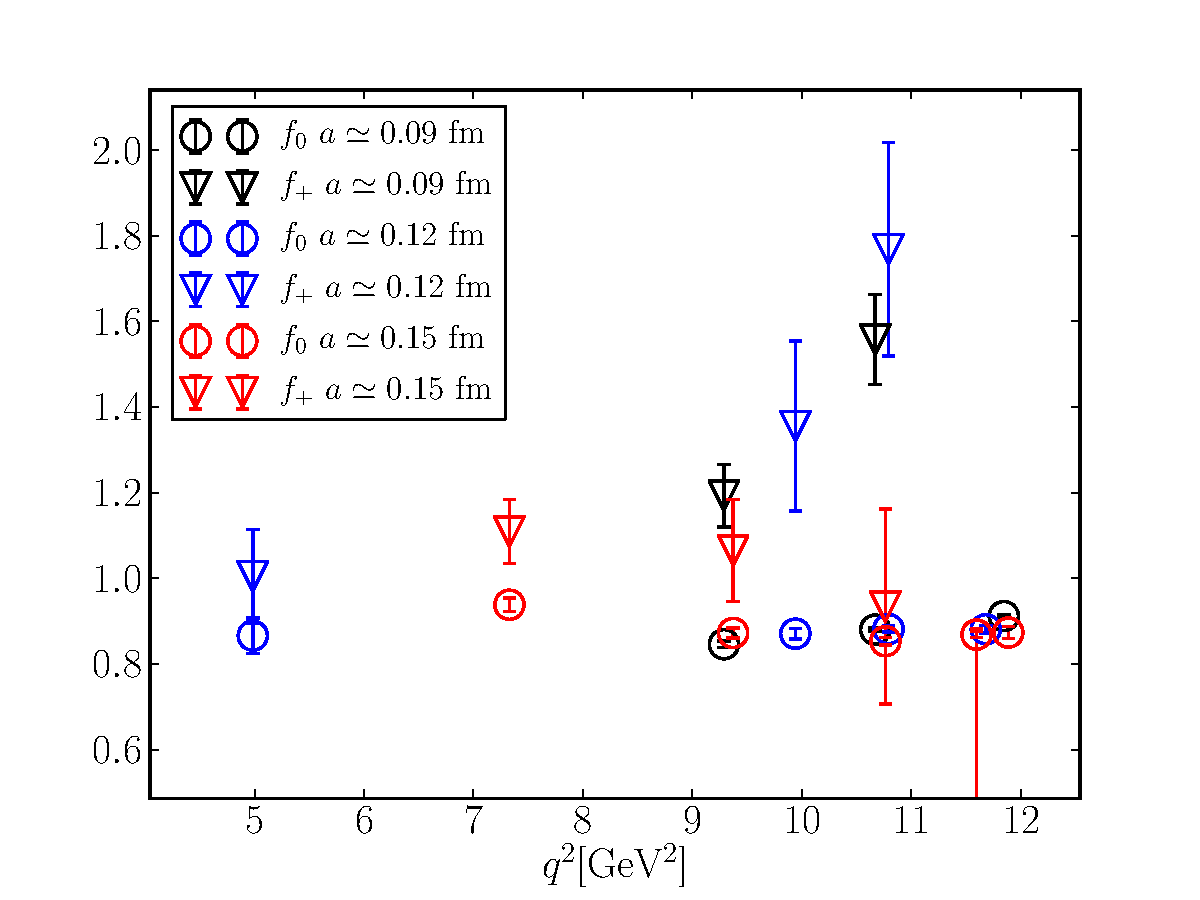
\includegraphics[width=1.0\textwidth]{images/nrqcd/BD_formfactors_fromV0S.pdf}
  \end{center}
  \caption{$B\to D$ form factors extracted from $\langle V_0 \rangle$ and $\langle S \rangle$. Clearly these results are nonsense. See text. \label{fig:f0fp_fromV0S}}
\end{figure}

Results from adopting this alternative approach (in the $B\to D$ case) is shown in fig. \ref{fig:f0fp_fromV0S}. One immediately notices that $f_+(q^2)$ results are diverging in the $|{\textbf{p}}_{D}| \to 0$ limit. Why this occurs can be seen by inspecting eq. \eqref{eq:fplus_badness}. For $f_+$ to remain finite, the difference between currents on the numerator must tend to zero at the same rate as ${\textbf{p}}_D^2$. Our results for the currents $\langle S \rangle$ and $\langle V_0 \rangle$ are not precise enough to produce the delicate cancellation required to accurately determine $f_+$ in the high $q^2$ region.

Let's summarize the situation. We have 3 currents, $\langle S \rangle$, $\langle V_0 \rangle$, and $\langle V_k \rangle$. We require input from two of these currents in order to determine the form factors. Large contributions to $\langle V_k \rangle$ may be being ignored, so at the moment we do not consider $\langle V_k \rangle$ a 'trustworthy' estimation of the continuum spacial vector current. Using only $\langle S \rangle$ and $\langle V_0 \rangle$ leads to a divergence of $f_+(q^2)$ as $q^2\to q^2_{\text{max}}$, so is also untenable. In the next section, we show an approach we attempted to finding new normalizations of these three currents such that all three can be 'trusted' as good approximations to the continuum current. One could then in principle use these trustworthy $\langle V_0 \rangle$ and $\langle V_k \rangle$ currents to extract the form factors.

\section{Non-Perturbative Renormalization using $B_c\to \eta_c$ Data}
\label{sec:Bcetac}

Here we define non-perturbative normalization constants $Z_J$ for the NRQCD-HISQ currents via 
\begin{align}
  \nonumber
	J &= ( 1 + z^J_0 \alpha_s )( J^{(0)} + J^{(1)} ) + \mathcal{O}(\, \alpha_s^2, \, (\Lambda_{\text{QCD}}/m_b)^2, \, ({\textbf{p}}/m_b)^2,\,\,\alpha_s \Lambda_{\text{QCD}} / m_b,\, \alpha_s {\textbf{p}}/m_b ) \\
	&\equiv Z_{J}( 1 + z^J_0 \alpha_s )( J^{(0)} + J^{(1)} ), \\ \nonumber &\quad\quad Z_{J} = 1 +  \mathcal{O}(\, \alpha_s^2, \, (\Lambda_{\text{QCD}}/m_b)^2, \, ({\textbf{p}}/m_b)^2,\,\,\alpha_s \Lambda_{\text{QCD}} / m_b,\, \alpha_s {\textbf{p}}/m_b ).
	\label{eq:overall}
\end{align}
The $Z_J$ factor compensates for the truncation of the series. One can imagine fixing $Z_J$ by demanding some property of $J$. One may be concerned that $Z_J$ is dependent on the spacial momenta in the current $Z_J=Z_J({\textbf{p}})$, however, we will see below that this variation is a negligable effect.

In this section, we outline an approach used to determine $Z_S$, $Z_{V_0}$ and $Z_{V_k}$. In this process we use NRQCD data from another HPQCD project of determining form factors for $B_c \to \eta_c l\nu$ decays \cite{Colquhoun:2016osw}. A schematic of how this is achieved is given in fig. \ref{fig:normalization_chain}. I thank Brian Colquhoun for supplying correlation functions from their calculation. The current in this calculation is the same as in the $B_{(s)}\to D_{(s)}l\nu$ calculation, so normalizations determined using this data can then be applied to the $B_{(s)}\to D_{(s)}l\nu$ calculation. I use the $B_c \to \eta_c l\nu$ data here since
\begin{itemize}
\item
  $B_c\to \eta_c$ correlators have much smaller statistical errors. This is because of the lack of the $s$ spectator quark, degradation of the signal/noise ratio is less severe (see sec. \ref{sec:signaldegredation}).
\item
  A heavy-HISQ determination of $B_c\to \eta_c$ form factors was also available from their project \cite{Colquhoun:2016osw}. This comes in useful in our approach to the normalization.
\end{itemize}
All analysis below is performed using data on the fine ensemble (set 2). In principle, it could be repeated for any other ensemble on which correlators for any $b\to c$ transition is available.

\begin{figure}[htb!]
\hspace{-5pt}
    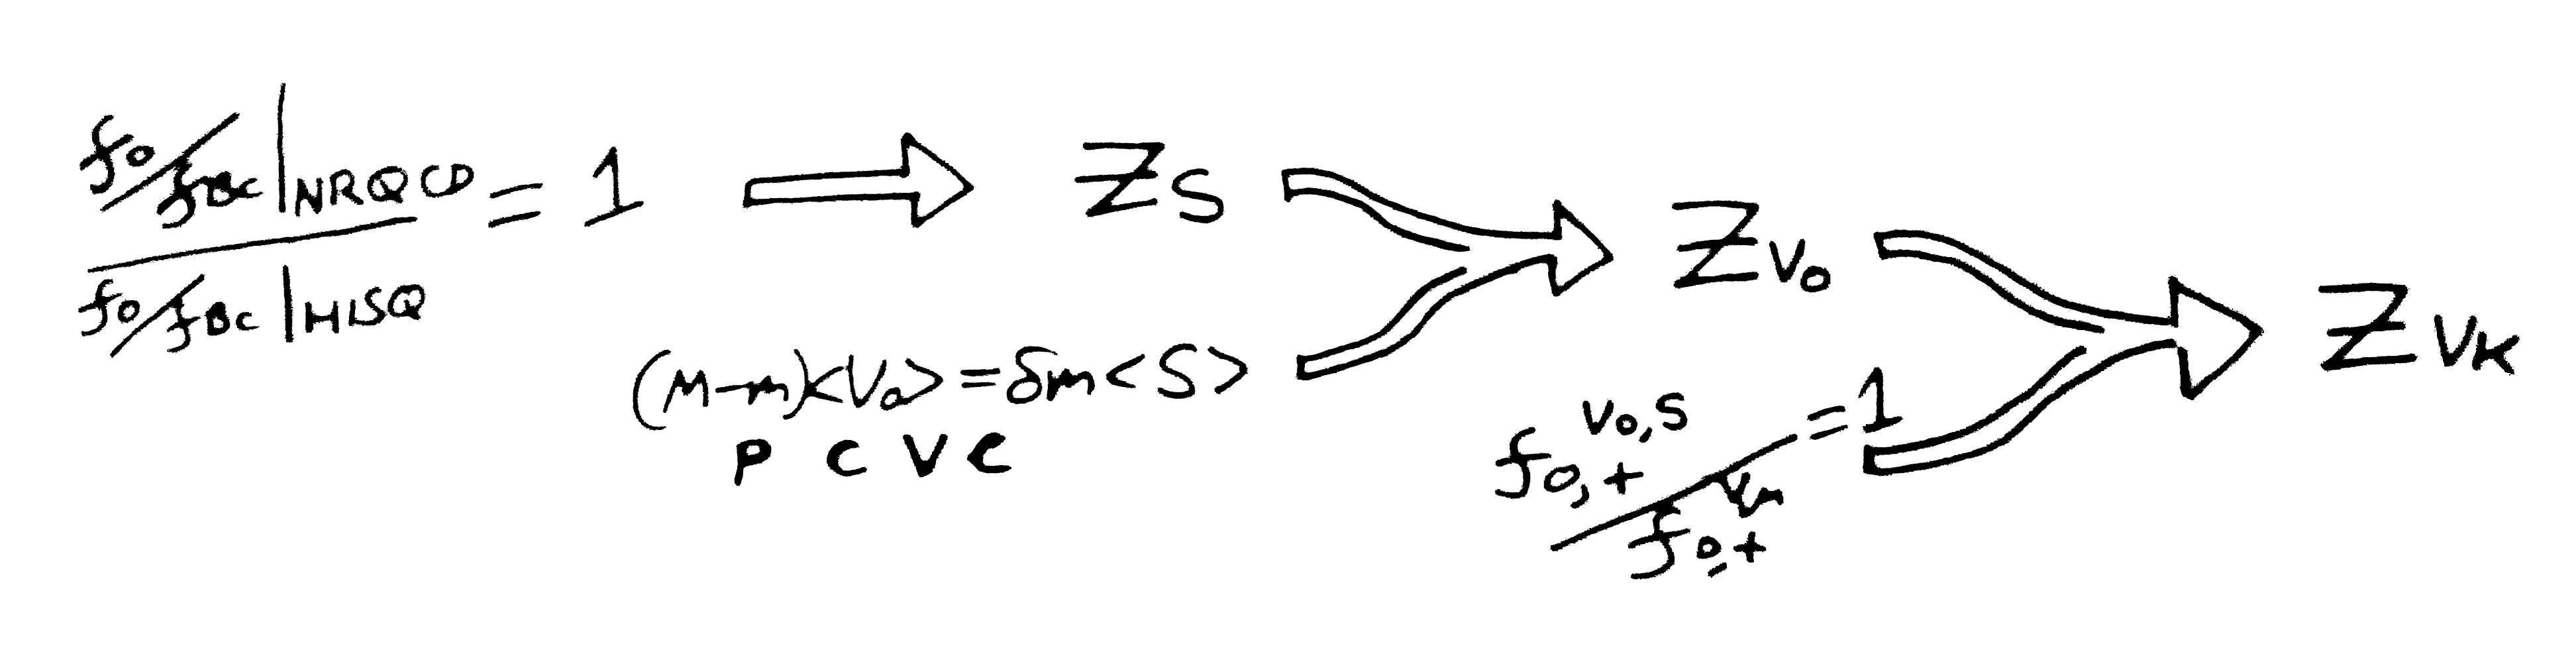
\includegraphics[width=1.0\textwidth]{images/nrqcd/normalization_chain.jpg}
  \caption{A schematic of the chain of steps towards normalizing the scalar, temporal vector and spacial vector NRQCD-HISQ currents. Details given in the next three sections; \ref{sec:Zs}, \ref{sec:ZV0} and \ref{sec:ZVk}. \label{fig:normalization_chain}}
\end{figure}

\subsection{$Z_S$}
\label{sec:Zs}

We have avaliable to us lattice results for $f_0(q^2)$ for a number of $q^2$ values spanning the entire $q^2$ range (including $q^2_{\text{max}}$ and $q^2=0$) from NRQCD-HISQ currents on the fine ensemble. We also have a determination of $f_{B_c}$ also from NRQCD-HISQ lattice currents on the same ensemble. We denote these finite-$a$ lattice results as $\hat{f}_0(q^2)$, $\hat{f}_{B_c}$. We also have a continuum-extrapolated heavy-HISQ result for $f_0(q^2)/f_{B_c}$, for a range of $q^2$ values also including $q^2_{\text{max}}$ and $q^2=0$. This is given in the form of this ratio since discretization effects largely cancel in this ratio improving the continuum extrapolation. Namely we have
\begin{align}
  {f_0(q^2_{\text{max}})\over f_{B_c}} = 2.104(36),\quad {f_0(0)\over f_{B_c}} = 1.288(42).
\end{align}
I thank Andrew Lytle for these results. Since $f_0\propto \langle S \rangle$, we can assert that $f_0 = Z_S \hat{f}_0$, i.e., the continuum $f_0$ contains the normalization that $\hat{f}_0$ is missing. Similarly for $\hat{f}_{B_c}$ and $Z_{A_0}$. Hence by demanding that the NRQCD-HISQ finite-$a$ results match the continuum heavy-HISQ results, we can find, for example
\begin{align}
  {Z_S \over Z_{A_0}}\bigg\vert_{q^2_{\text{max}}} = {f_0(q^2_{\text{max}})/f_{B_c}\over \hat{f}_0(q^2_{\text{max}})/\hat{f}_{B_c}} = 0.995(15).
\end{align}
As a test to see if $Z_S$ varies with ${\textbf{p}}$, we can compare this result to an analagous approach at $q^2=0$;
\begin{align}
  {Z_S \over Z_{A_0}}\bigg\vert_{q^2=0} = {f_0(0)/f_{B_c}\over \hat{f}_0(0)/\hat{f}_{B_c}} = 0.962(33).
\end{align}
A similar approach cannot be applied for $Z_{V_0}$ or $Z_{V_k}$, since $f_0$ has a complicated relationship to both $\langle V_0 \rangle$ and $\langle V_k \rangle$ that varies with $q^2$, so it is not clear how one attribute discrepancies between $\hat{f}_0/\hat{f}_{B_c}$ and $f_0/f_{B_c}$ to $Z_{V_0}$ and $Z_{V_k}$.

The comparison of these two ratios at $q^2_{\text{max}}$ and $q^2=0$ show that any variaton is small in comparison to statistical errors. We can absorb the variation in ${\textbf{p}}$ into a subleading term in the scalar current by demanding that $Z_{S}/Z_{A_0}|_{q^2_{\text{max}}} = Z_{S}/Z_{A_0}|_{q^2=0}$. Redefine the scalar current according to:
\begin{align}
 S = Z_{S} \left[ (1 + z^{S}_0 \alpha_s)( V_0^{(0)} - V_0^{(1)} ) + \alpha_s z^{S}_2 V_0^{(2)} \right].
\end{align}
We can determine $z_2^S$ by demanding that $Z_S$ does not vary between $q^2_{\text{max}}$ and $q^2=0$. This is equivilant to the $V_0^{(2)}$ term absorbing all of the variation in the normalization on ${\textbf{p}}$, which one would expect since this current is proportional to the spacial momentum in the $c$-quark.

By defining $\hat{f}_2$ to be $\hat{f}_0$ but with $(1+\alpha_s z_0^S)( V_0^{(0)} - V_0^{(1)} )$ replaced with $\alpha_s V_0^{(2)}$, we can write:
\begin{align}
	{Z_{A_0}\over Z_{S}} = { ( \hat{f}_0 + z^S_2 \hat{f}_2 )/ \hat{f}_{B_c}  \over f_0/f_{B_c} } \equiv \left({Z_{A_0}\over Z_{S}}\right)^{(0,1)} + z^S_2 \left({Z_{A_0}\over Z_{S}}\right)^{(2)}.
\end{align}
With this further definition, and demanding that ${Z_{A_0}/ Z_{S}}|_{q^2_{\text{max}}} = {Z_{A_0}/ Z_{S}}|_{q^2=0}$, we end up with
\begin{align}
	z^S_2 = { \left({Z_{A_0}\over Z_{S}}\right)^{(0,1)}\big\vert_{q^2=0} - \left({Z_{A_0}\over Z_{S}}\right)^{(0,1)}\big\vert_{q^2_{\text{max}}}
\over \left({Z_{A_0}\over Z_{S}}\right)^{(2)}\big\vert_{q^2_{\text{max}}} - \left({Z_{A_0}\over Z_{S}}\right)^{(2)}\big\vert_{q^2=0} }
 = -1.1(1.5).
\end{align}
Now that we are able to include $V_0^{(2)}$ in the scalar current, we can consider the scalar current normalized up to $\mathcal{O}(\alpha_s^2, \,(\Lambda_{\text{QCD}}/m_b)^2, \,({\textbf{p}}/m_b)^2, \alpha_s\Lambda_{\text{QCD}}/m_b )$. We can use
\begin{align}
  S = (1+z_0^S\alpha_s)( V_0^{(0)} - V_0^{(1)} ) + z_2^s\alpha_s V_0^{(2)} + \mathcal{O}(\alpha_s^2, \,(\Lambda_{\text{QCD}}/m_b)^2, \,({\textbf{p}}/m_b)^2,\,\, \alpha_s\Lambda_{\text{QCD}}/m_b )
\end{align}
Yes, we have not strictly determined $Z_S$ in this case, but we will for the vector currents). The next steps are essentially to match results using the vector currents to this newly normalized scalar current, meaning the vector currents will be normalized up to $\mathcal{O}(\alpha_s^2, \,(\Lambda_{\text{QCD}}/m_b)^2, \,({\textbf{p}}/m_b)^2 )$, hence we have theoretically accounted for the large subleading pieces in the spacial vector current, since we have accounted for $\alpha_s{\textbf{p}}/m_b$ order terms.

\subsection{$Z_{V_0}$}
\label{sec:ZV0}

We normalize the temporal vector current via its PCVC relation with the now correctly normalized scalar current.

This also has the benefit of partially removing the $f_+(q^2)$ divergence as ${\textbf{p}}^2_{\eta_c}\to 0$ when extracted from $\langle V_0 \rangle$ and $\langle S \rangle$. We can see this by inspecting the expression for $f_+(q^2)$ (Eq. \eqref{eq:fplus_badness}) in terms of $\langle S \rangle$ and $\langle V_0 \rangle$ as ${\textbf{p}}_{\eta_c}^2 \to 0$. The numerator becomes $(m_b-m_c) \langle S \rangle - (M_{B_c}-M_{\eta_c}) \langle V_0 \rangle$, which vanishes when the PCVC relation is satisfied. So one would expect if we renormalize one of the currents so the Ward identity is satisfied (at $q^2_{\text{max}}$), this divergence should be removed or at least reduced.

\begin{figure}[htb!]
\centering
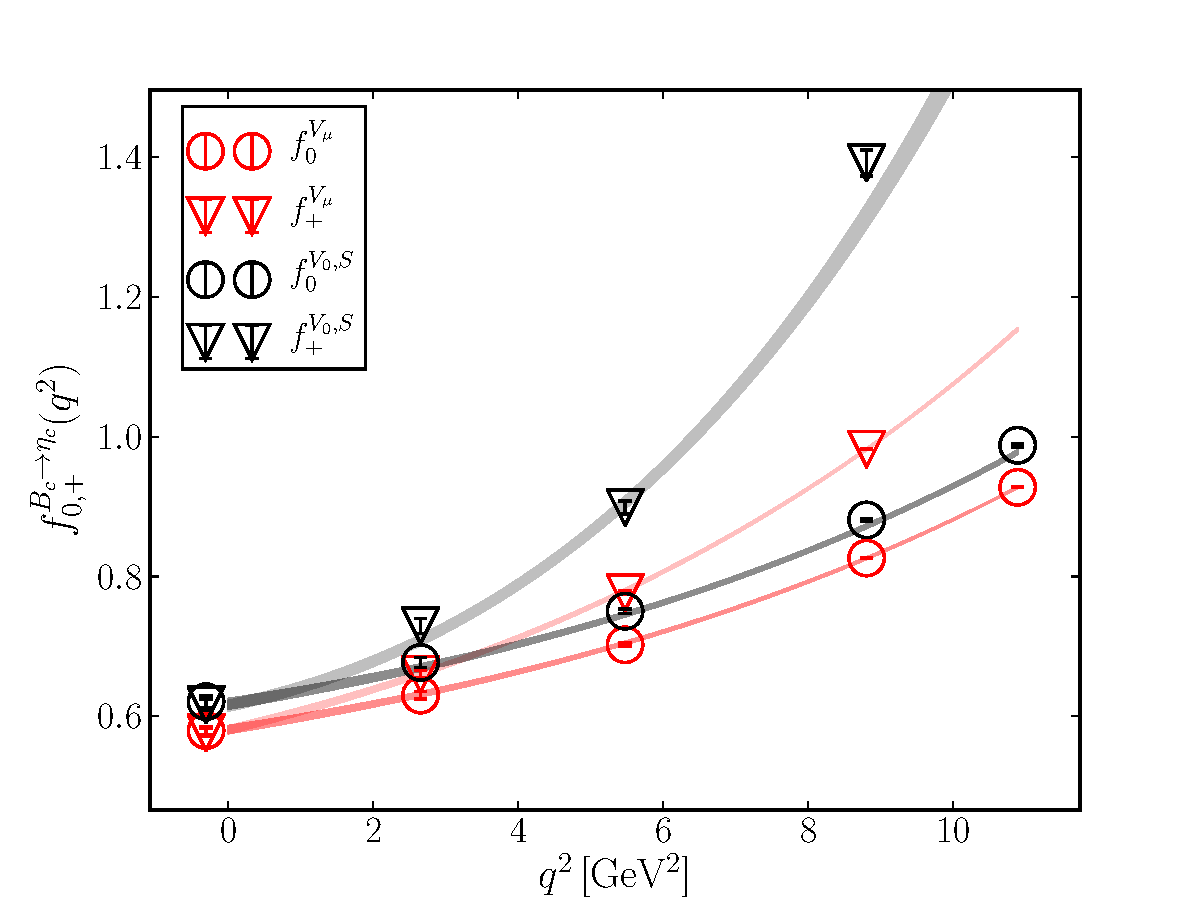
\includegraphics[scale=0.55]{images/nrqcd/Bcetac_bothways_1.pdf}
\caption{Comparison of form factors from $\langle V_0 \rangle, \langle S \rangle$ and $\langle V_0 \rangle,\langle V_k \rangle$, no additional normalizations. The bands show the resuls of fitting the data to the BGL parameterization \eqref{eq:zexpansion}, where coefficients $a^{0,+}_n$ are fit parameters. \label{fig:naive}}
\end{figure}

Hence we should normalize the temporal vector current using the already normalized scalar density. So to satisfy the PCVC, Multiply $\langle V_0 \rangle$ by 
\begin{align}
	Z_{V_0} = {m_b-m_c \over M_{B_c}-M_{\eta_c} } { \langle S \rangle \over \langle V_0 \rangle }\Big\vert_{q^2_{\text{max}}} = 1.0661(36).
	\label{eq:Zward}
\end{align}
This seems to deal with the $f_+$ divergence. Fig. \ref{fig:naive} compares form factors determined using $\langle V_0 \rangle$, $\langle S \rangle$, and $\langle V_0 \rangle$, $\langle V_k \rangle$, {\textit{before}} imposing $Z_{V_0}$, and Fig. \ref{fig:Zward} shows the same {\textit{after}} $\langle V_0 \rangle$ has been multiplied by $Z_{V_0}$.
\begin{figure}[htb!]
\centering
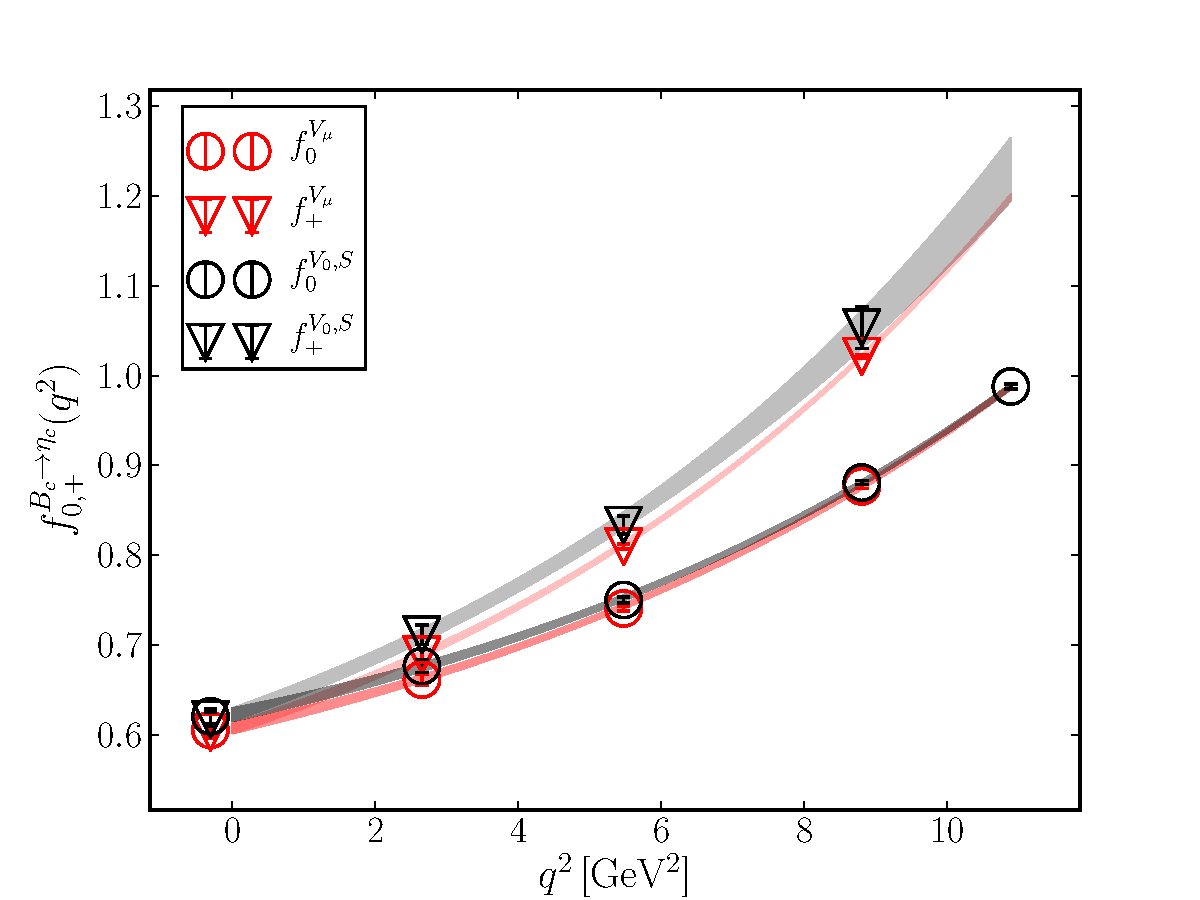
\includegraphics[scale=0.55]{images/nrqcd/Bcetac_bothways_2.pdf}
\caption{Comparison of form factors from $\langle V_0 \rangle,\langle S \rangle $ and $\langle V_0\rangle,\langle V_k\rangle$, $\langle V_0\rangle$ is mutliplied by $Z_{V_0}$ given in \eqref{eq:Zward}. The bands show the resuls of fitting the data to the BGL parameterization \eqref{eq:zexpansion}, where coefficients $a^{0,+}_n$ are fit parameters. \label{fig:Zward}}
\end{figure}
Unfortunately the same technique does not solve the diverging $f_+$ issue in the $B_{(s)}\to D_{(s)}$ case, the statistics are not as good so the divergence is too severe. 

\subsection{$Z_{V_k}$}
\label{sec:ZVk}

We can determine a $Z_{V_k}$ by demanding that $f_{0,+}^{V_0,S}/f_{0,+}^{V_{\mu}}=1$, with the knowledge that $\langle V_0 \rangle, \langle S \rangle$ require no further normalization. This can be done with both $f_+$ and $f_0$, at any $q^2$;
\begin{align}
	Z_{V_k} &= 1 + {f_+^{V_0,S} - f_+^{V_{\mu}} \over R_{+k} \langle V_k \rangle }  \\
	&= 1 + {f_0^{V_0,S} - f_0^{V_{\mu}} \over R_{0k} \langle V_k \rangle },
\end{align}
where the $R$'s are some kinematic gunk: $R_{+k} = ( M_{B_c} - E_{\eta_c} )/2M_{B_c}{\textbf{p}}_{\eta_c}/\sqrt{3}$, \\ $R_{0k} = R_{+k} - {( M_{B_c}^2-M_{\eta_c}^2 )(M_{B_c}-E_{\eta_c})/2M_{B_c} {\textbf{p}}_{\eta_c}/q^2\sqrt{3}}$. The results are shown in fig. \ref{fig:ZVk}.
\begin{figure}[htb!]
\centering
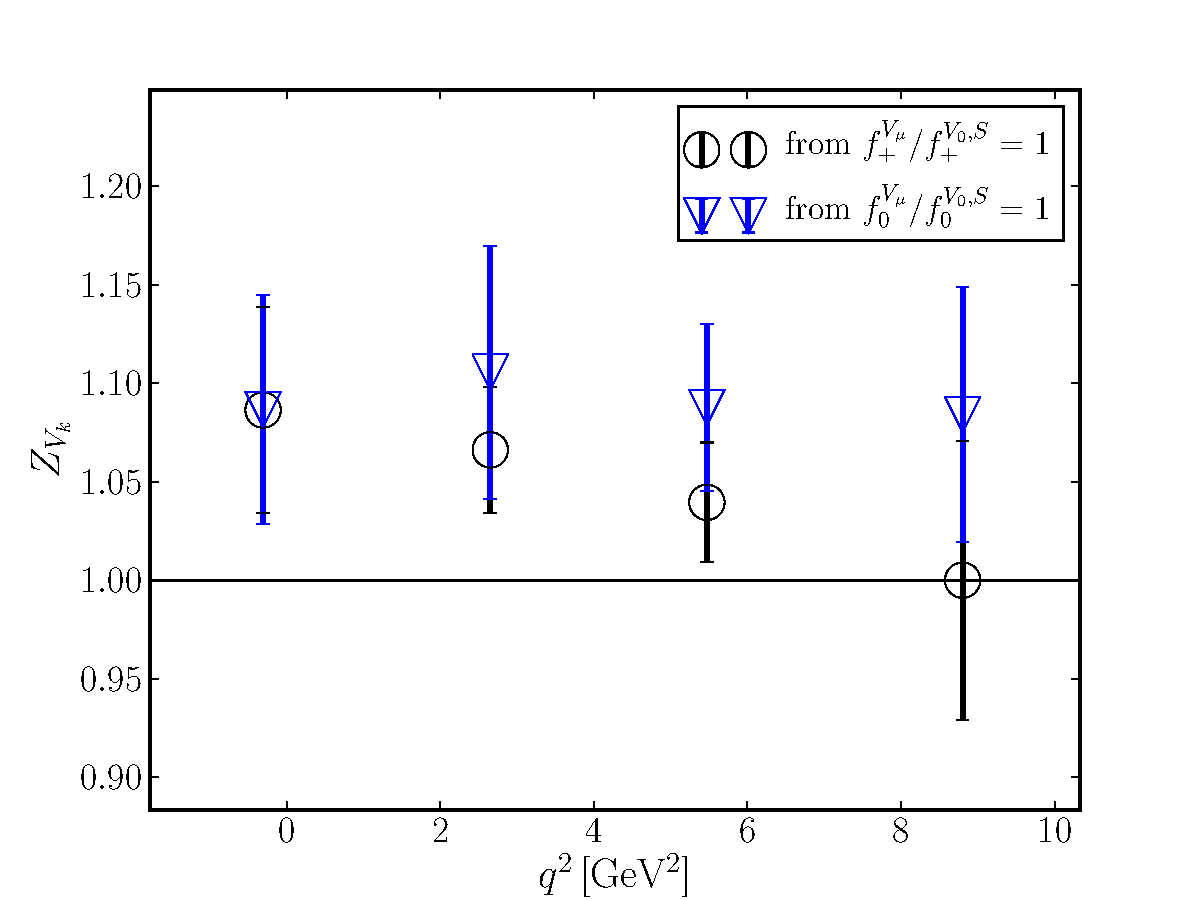
\includegraphics[scale=0.5]{images/nrqcd/ZVk.pdf}
\caption{$Z_{V_k}$ from constraining form factors to be the same from $\langle V_0 \rangle,\langle S \rangle$ and $\langle V_0 \rangle,\langle V_k \rangle$}
\label{fig:ZVk}
\end{figure}
The fact that these are not varying by a statistically significant extent in $q^2$ implies that the spacial vector normalization does not vary strongly in ${\textbf{p}}_{\eta_c}$. Hence, since these are all estimates of the same value, we can average over them to get
\begin{align}
	Z_{V_k} = 1.070(36).
\end{align}
When this normalization is given to $\langle V_k \rangle$, the $B_c\to\eta_c$ form factors from the two methods become consistent, see Fig. \ref{fig:identicle}.

\begin{figure}[htb!]
\centering
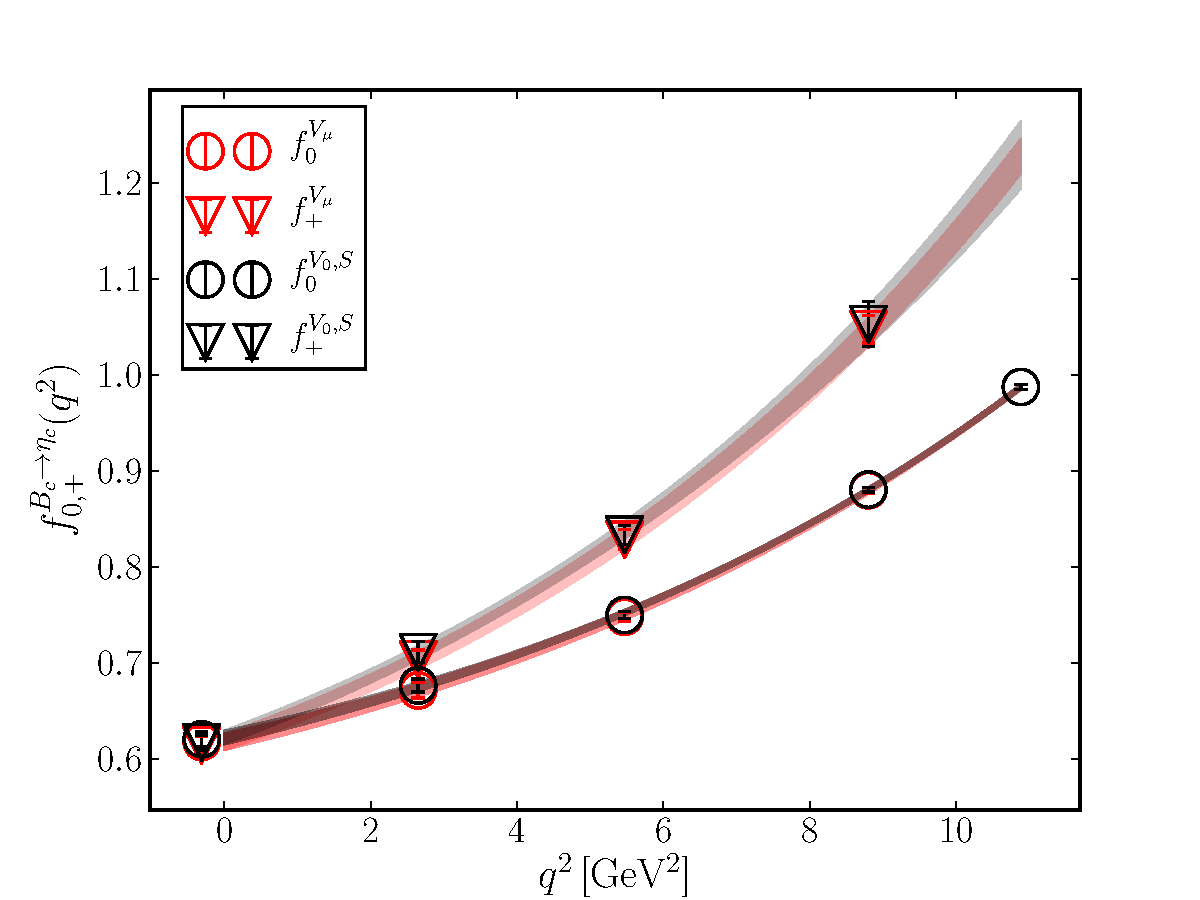
\includegraphics[scale=0.55]{images/nrqcd/Bcetac_bothways_3.pdf}
\caption{Comparison of form factors from $\langle V_0 \rangle, \langle S \rangle$ and $\langle V_0 \rangle,\langle V_k \rangle$, with $\langle V_0 \rangle$ normalized with $Z_{V_0}$ and $\langle V_k \rangle$ normalized with $Z_{V_k}$. The bands show the resuls of fitting the data to the BGL parameterization \eqref{eq:zexpansion}, where coefficients $a^{0,+}_n$ are fit parameters. \label{fig:identicle}}
\end{figure}

One could imagine using these normalizations $Z_{V_0}$ and $Z_{V_k}$ in the $B_{(s)}\to D_{(s)}$ calculation. The errors of this normalization are around $4\%$, which would push the final results of the $B_{(s)}\to D_{(s)}$ study up to the $5-10\%$ range. At present this level of precision is not competitive in comparison to other calculations of these quantities.

\section{Conclusion of NRQCD work}

As mentioned in the introduction - the main takehome of this thesis is that using NRQCD (namely NRQCD-HISQ currents) to compute form factors for $b\to c$ transitions, is far from optimal. 

We rely here on truncations in many different interlocking series ($1/m_b, \alpha_s,\alpha_s/m_b,...$), which may leave out important information. The terms in the series we {\textit{do}} have access to rely on perturbation theory via the matching factors. Some progress was made to normalize currents non-perturbatively in the above work, but our results fall short of what would be required to obtain precise continuum results.

I hope that in reading this chapter you experienced a similar feeling of confusion and anxiety to what I felt when carrying out this work. It was only after many months of grappling with the problems of these calculations that we decided to put them aside and attempt instead the heavy-HISQ approach from scratch. Reading the following two chapters, both dedicated to successful heavy-HISQ studies, will feel like a warm bath in comparison to the NRQCD experience. The heavy-HISQ approach is in contrast very elegant, contains far assumptions, and results in cleaner signals.
 % NRQCD studies
\chapter{$B_s\to D_s^*l\nu$ Axial Form Factor at Zero Recoil from Heavy-HISQ}
\label{chap:BsDsstar}

This chapter concerns the simpler of our two heavy-HISQ studies, the calculation of the $B_s\to D^*_sl\nu$ axial form factor at zero recoil, $h^s_{A_1}(1)$. We give this quantity the superscript $s$ to differentiate it from the quantity more commonly referred to as $h_{A_1}(1)$, the zero recoil axial form factor for $B\to D^*l\nu$ decays.

I will briefly review the definition of this form factor (at zero recoil) for ease of reading. The differential decay rate for the $\bar{B}_s^0\to D_s^{*+} l^- \bar{\nu}_l$ decay is given in the SM by
\begin{align}
  {d \Gamma \over dw} &(\bar{B}_s^0\to D_s^{*+} l^- \bar{\nu}_l) = {G_F^2 M_{D_s^*}^3 | \bar{\eta}_{\text{EW}} V_{cb} |^2 \over 4\pi^3}
\\  &\times(M_{B_s}^2-M_{D_s^*}^2) \sqrt{w^2-1} \chi(w) | \mathcal{F}^{B_s\to D_s^*}(w) |^2. \nonumber
\end{align}
where $w = v_{B_s} \cdot v_{D^*_s}$, $v_M = p_M/M_M$ is the 4-velocity of a $M$-meson, and $\chi(w)$ is a known function of $w$ (see for example appendix G of \cite{Harrison:2017fmw}). $\bar{\eta}_{\text{EW}}$ accounts for electroweak corrections due to diagrams where photons or $Z$s are exchanged in addition to a $W^-$, as well as the Coulomb attraction of the final-state charged particles \cite{SIRLIN198283,Ginsberg1968,PhysRevD.41.1736}. The differential decay rate for the $B_s^0\to D_s^{*-} l^+ \bar{\nu}_l$ decay is identical.

The form factor $\mathcal{F}^{B_s\to D_s^*}(w)$ is a linear combination of hadronic form factors that parameterize the vector and axial-vector matrix elements between initial and final state hadrons. At zero recoil ($w=1$), the vector matrix element vanishes, the axial-vector element simplifies to
\begin{align}
  \langle D^*_s(\epsilon)| A_{\mu} | B_s \rangle &= 2 \sqrt{M_{B_s}M_{D^*_s}}\,\, h^s_{A_1}(1) \epsilon^{*}_{\mu}\,,
\end{align}
and $\mathcal{F}^{B_s\to D_s^*}(w)$ reduces to
\begin{align}
  \mathcal{F}^{B_s\to D_s^*}(1) = h^s_{A_1}(1)\,.
\end{align}
Our goal is to compute $h^s_{A_1}(1)$.

All we need to do this is the matrix element $\langle D^*_s(\epsilon)| A_{\mu} | B_s \rangle$ with both the $B_s$ and $D_s^*$ at rest, with the $D_s^*$ polarization $\epsilon$ in the same direction as the axial current.

\section{Motivation}
\label{sec:BsDsstar_intro}

$B\to D^{*} l \nu$ decays supply one of the three methods used for precisely determining the CKM element $|V_{cb}|$ \cite{Schroder:1994aj,PhysRevLett.64.2117,PhysRevD.43.651,ALBRECHT1992195,Barish:1994mu,BUSKULIC1996449,Buskulic:1994dz,Abbiendi:2000hk,Abreu:2001ic,Adam:2002uw,Abdallah:2004rz,Aubert:2007rs,Aubert:2007qs,Aubert:2008yv,Dungel:2010uk,Abdesselam:2017kjf,Bailey:2014tva,Abdesselam:2018nnh}.
Measurements of branching fractions are extrapolated through $q^2$ to the zero recoil point to deduce $|h_{A_1}(1)V_{cb}|$, since $h_{A_1}(1)$ is the only form factor contributing at zero recoil. Then an SM determination of $h_{A_1}(1)$ (via Lattice QCD \cite{Bailey:2014tva,Harrison:2017fmw}) can be divided out to infer $|V_{cb}|$.

A similar process that could also be used to determine $|V_{cb}|$, and test the SM, is $\bar{B}_s \to D^*_s l\bar{\nu}_l$. There is at time of writing no published measurements of this decay, but it is feasible to measure such a decay at a detector like LHCb. This decay is also attractive from the Lattice QCD side.
The absence of valence light quarks means lattice results have smaller statistical errors, are less computationally expensive, a simpler chiral extrapolation to the physical light mass, and negligible finite volume effects. This makes the $\bar{B}_s \to D^*_s l\bar{\nu}_l$ both a useful test bed for lattice techniques (that may be later used to study $\bar{B} \to D^* l \bar{\nu}_l$ decays), and a key decay for future $|V_{cb}|$ determinations and tests of the SM.

Chiral symmetry implies that form factors for decays such as $B_s \to D^*_s$ and $B \to D^*$ are insensitive to the mass of the spectator quark, implying that form factors for these two decays are approximately equal \cite{Laiho:2005ue}. This was seen in the recent lattice calculation \cite{Harrison:2017fmw} that found $h_{A_1}(1) / h^s_{A_1}(1) = 1.013(14)_{\text{stat}}(17)_{\text{sys}}$. We can then expect to learn about $B\to D^*$ by studying $B_s\to D_s^*$. We perform a further test of this claim that $B\to D^*\sim B_s\to D_s^*$, in the context of our formalism, in this study.

Lattice calculations of the $B_{(s)} \to D_{(s)}^*$ form factors at zero recoil have so far been performed by two collaborations. The Fermilab Lattice collaboration produced $h_{A_1}(1)$ in \cite{Bailey:2014tva}. HPQCD computed both $h_{A_1}(1)$ and $h_{A_1}^s(1)$ in \cite{Harrison:2017fmw}. The RBC/UKQCD \cite{Flynn:2016vej} and LANL-SWME \cite{Bailey:2017xjk} collaborations are also working towards lattice determinations of these form factors.

%% Lattice calculations of the $B_{(s)} \to D_{(s)}^*$ form factors at zero recoil have been performed by a number of collaborations. RBC/UKQCD is working towards determining the form factors using their 2+1 gauge ensembles, Domain Wall light, strange and charm quarks, and Wilson-type bottom quarks \cite{Flynn:2016vej}. The FNAL/MILC collaboration produced the $B\to D^*$ form factor at zero recoil on the 2+1 MILC ensembles using ASQTAD light and strange quarks and Wilson-type charm and bottom quarks \cite{Bailey:2014tva}. HPQCD has produced $B_{(s)}\to D_{(s)}^*$ form factors at zero recoil, on the 2+1+1 MILC ensembles, HISQ light, strange and charm quarks, and NRQCD bottom quarks \cite{Harrison:2017fmw}.

The presence of heavy quarks is a large consideration in designing a lattice calculation (as discussed in Sec. \ref{sec:lattice_heavyquarks}). A $b$ quark introduces discretization effects of size $(am_b)^n$ where $n$ is a positive integer dependent on the choice of action. To avoid such potentially large discretization effects, most lattice studies (including all of those mentioned in the previous paragraph), use some EFT approach for simulating heavy quarks. The Fermilab Lattice, RBC/UKQCD, and LANL-SWME calculations all used some variation of the Fermilab action \cite{Wilson:1977xx,SHEIKHOLESLAMI1985572,ElKhadra:1996mp} to simulate $c$ and $b$ quarks. The HPQCD calculation used the NRQCD action \cite{Lepage:1992tx} for $b$ quarks. 

To relate the results from these approaches to full continuum QCD, each of the above studies requires perturbative matching of lattice currents to continuum QCD. The matching has only been performed to 1-loop, leading to each having matching errors as a key uncertainty. The use of NRQCD-HISQ currents in the HPQCD calculation brings in matching errors of $\order{\alpha_s^2,\alpha_s \Lqcd / m_b, (\Lqcd / m_b )^2}$. It is difficult to estimate the size of matching errors in lattice NRQCD, so to be conservative a large matching error was assigned to the result. This error contributes $\sim 80\%$ of the full error budget. The use of the Fermilab action in the Fermilab Lattice calculation leads to $\order{\alpha_s^2}$ errors. They avoid this issue to a large extent by analysing only ratios of correlation functions, however, the matching still contributes $\sim 30\%$ to the final error. %The final results for the RBC/UKQCD calculation are not yet published, however, they report requiring matching factors that are only known to tree level, which could cause errors as large as $\order{\alpha_s}$ in the final result.

In this chapter, we report details and results of the first calculation of the $B_s\to D^*_s$ form factor at zero recoil using an approach free of perturbative matching. 

Since the $B_s\to D_s$ form factor is approximately equal to the $B\to D$ form factor, and our results are non-perturbatively renormalised, this calculation can be seen as a check of the normalisation of the Fermilab Lattice and HPQCD determinations of $h_{A_1}(1)$ that contributed to $|V_{cb}|_{\text{excl}}$ (see Sec. \ref{sec:Vcb}). %While producing a quantity less relevant to current phenomenology than the $B\to D^*$ form factor, this calculation can be seen as a proof-of-principle for the heavy-HISQ approach. 

Using the heavy-HISQ approach has the added benefit of elucidating the dependence of form factors on heavy quark masses, meaning we can test expectations from Heavy Quark Effective Theory (HQET). In this study, we produce an estimate of the HQET low energy constants $l_{V,A,P}$ associated with the $B_s \to D_s^*$ form factor at zero recoil.

\section{Calculation Details}
\label{sec:BsDsstar_deets}

\subsection{Lattice Setup}

We used the MILC gluon field configurations detailed in Sec. \ref{sec:MILCensembles} \cite{Bazavov:2010ru,Bazavov:2012xda}. We used sets 2-5 in Table \ref{tab:ensembles}, i.e., the fine, fine-physical, superfine and ultrafine ensembles. Table \ref{tab:BsDsensembles} gives the valence quark masses we used in the generation of quark propagators. In three of the four ensembles (fine,superfine and ultrafine), the bare light mass is set to $m_{l0}/m_{s0} = 0.2$. The fact that the $m_{l0}$ value is unphysically high is expected to have a small effect on $h^s_{A_1}(1)$, due to the lack of valence light quarks, and previous experience of the dependence of $h_{A_1}^s(1)$ on $m_{l0}$ \cite{Harrison:2017fmw}. The small effect due to the unphysical $m_{l0}$ is quantified by including the fine-physical ensemble with physical $m_{l0}$, and corrected for.

We used a number of different masses for the valence heavy quark. This is in order to resolve the dependence of $h_{A_1}^s(1)$ on the heavy mass so that extrapolation to $m_h=m_b$ can be performed. By varying the heavy mass both within ensembles and between ensembles, we can resolve both the discretization effects that grow with large ($am^{\text{val}}_{h0} \lesssim 1$) masses and the physical dependence of the continuum form factor on $m_h$.

A considerable benefit to using unphysically light heavy quarks is that it reduces the signal/noise degradation in the correlation functions in comparison to using the physical $b$ mass (as in e.g. the NRQCD approach). When using NRQCD, the large noise due to the heavy $b$-quark necessitated the computation of many correlation functions with different smeared operators in order to boost statistics. This is not necessary in the heavy-HISQ setting, we used only local creation/annihilation operators.

\begin{table}
  \begin{center}
    \begin{tabular}{c c c c c c c}
      \hline
      set & handle & $am_{s0}^{\text{val}}$ & $am_{c0}^{\text{val}}$ & $am^{\text{val}}_{h0}$ & $n_{\text{cfg}}\times n_{\text{src}}$ & $T/a$ \\ [0.5ex]
      \hline
      2 & \bf{fine} & 0.0376 & 0.45 
      & 0.5, 0.65, 0.8 & $938\times 8$ & 14,17,20 \\ [1ex]
      3 & \bf{fine-physical} & 0.036 & 0.433 
      & 0.5, 0.8 & $284\times 4$ & 14,17,20 \\ [1ex]
      4 & \bf{superfine} & 0.0234 & 
      0.274 & 0.427, 0.525, 0.65, 0.8 & $250\times 8$ & 22,25,28  \\ [1ex]
      5 & \bf{ultrafine} & 0.0165 
      & 0.194 & 0.5, 0.65, 0.8 & $249\times 4$ & 31,36,41\\ [1ex]
      \hline
    \end{tabular}
  \end{center}
  \caption{Parameters relevent to our calculation. Columns 3 and 4 give the $s$ and $c$ valence quark masses, these values were tuned in \cite{Chakraborty:2014aca} to reproduce the correct $\eta_s$ and $\eta_c$ masses. We used a number of heavy quark masses to assist the extrapolation to the physical $b$ mass, given in column 5. Column 6 gives the number of gauge configurations ($n_{\text{cfg}}$) and the number of $t_0$ choices ($n_{\text{src}}$) used. Column 7 gives the temporal separations between source and sink, $T/a$, of the 3-point correlation functions computed on each ensemble.}
  \label{tab:BsDsensembles}
\end{table}

As detailed in Sec. \ref{sec:staggeredcorrelators}, staggered correlation functions are built by a combination of staggered propagators $g(x,y)$ and staggered phases. In this calculation we only need local (non-point-split) operators, this is an advantage since point-split operators lead to correlation functions noisier than local operators. 

We computed a number of correlation functions on each ensemble. To generate these correlators we used random wall sources, and used extended sources for the 3-point correlators, as described in Sec. \ref{sec:staggeredcorrelators}. First, we computed 2-point correlation functions between zero-momentum eigenstates, objects of the form
\begin{align}
  C_{M}(t) =& \langle \Phi_M (t) \Phi_M^{\dagger}(0) \rangle\,, \\ 
  &\Phi_M(t) = \sum_{{\bf{x}}} \bar{q}({\bf{x}},t) \Gamma q'({\bf{x}},t), \nonumber\,.
\end{align}
where $\langle \rangle$ represents a functional integral, $q,q'$ are valence quark fields of the flavours the $M$ meson is charged under, and $\Gamma$ is the spin-taste structure of $M$. I set $t_0=0$ here for notational simplicity. We computed these for all $t$ values, i.e. $0\leq t \leq T_{\text{lat}}$. 

We computed correlation functions for a heavy-strange pseudoscalar, $H_s$, with spin-taste structure $(\gamma_5\otimes \gamma_5)$. In terms of staggered propagators, this takes the form
\begin{align}
  C_{H_s}(t) = \sum_{\bf{x},\bf{y}} \left\langle \text{Tr}_c\left[ g_h(x,y) g_s^{\dagger}(x,y) \right] \right\rangle,
  \label{eq:pseudoscalar_corrs_BsDsstar}
\end{align}
where $g_q(x,y)$ is a staggered propagator for flavour $q$, and the trace is over color. Here $x_0=0$ and $y_0=t$. We also computed correlators for a charm-strange vector meson $D_s^*$, with structure $(\gamma_{\mu}\otimes \gamma_{\mu})$, using
\begin{align}
  C_{D_s^*}(t) = \sum_{\bf{x},\bf{y}} (-1)^{x_{\mu}+y_{\mu}} \left\langle \text{Tr}_c\left[ g_c(x,y) g_s^{\dagger}(x,y) \right] \right\rangle.
\end{align}

In order to non-perturbatively renormalise the axial vector current, we computed correlation functions for goldstone and non-goldstone pseudoscalar and heavy-charm mesons, denoted $H_c$ and $\hat{H}_c$ respectively. $H_c$ has spin-taste structure $(\gamma_5\otimes \gamma_5)$ and $\hat{H}_c$ has structure $(\gamma_5\gamma_0\otimes \gamma_5\gamma_0)$. $H_c$ correlators are computed using \eqref{eq:pseudoscalar_corrs_BsDsstar} (with $g_s$ replaced with $g_c$), while $\hat{H}_c$ correlators are given by
\begin{align}
  C_{\hat{H}_c}(t) = \sum_{\bf{x},\bf{y}}(-1)^{\bar{x}_0+\bar{y}_0} \left\langle \text{Tr}_c\left[ g_h(x,y) g^{\dagger}_c(x,y) \right] \right\rangle,
\end{align}
where I'm using the notation $\bar{z}_{\mu} = \sum_{\nu\neq\mu} z_{\nu}$.

The heavy-mass extrapolation requires masses of $\eta_h$ mesons, heavy-heavy pseudoscalars artificially forbidden to annihilate. To quantify mistuning of the charm and strange quark masses, we also require masses for $\eta_c$ and $\eta_s$ mesons, identical to $\eta_h$ with $h$ replaced $c$ and $s$ quarks respectively. We computed correlators for each of these, using a spin-taste $(\gamma_5\otimes \gamma_5)$, taking the form of \eqref{eq:pseudoscalar_corrs_BsDsstar}.

We then generate the 3-point correlation functions
\begin{align}
  C_3(t,T) =& \sum_{{\bf{y}}} \langle \Phi_{D_s^*(\epsilon)}(T)\, A_{\mu}({\bf{y}},t) \,\Phi_{H_s}(0) \rangle, \\
  &A_{\mu}({\bf{y}},t) = \bar{c}({\bf{y}},t) \gamma_5\gamma_{\mu} h({\bf{y}},t). \nonumber
\end{align}
In terms of the staggered formalism, the $H_s$ source is given structure $(\gamma_5\otimes \gamma_5)$, the $D_s^*$ sink is given $(\gamma_{\mu}\otimes \gamma_{\mu})$, and the current insertion $(\gamma_5\gamma_{\mu}\otimes \gamma_5\gamma_{\mu})$. In terms of staggered propagators this is given by
\begin{align}
  C_3(t,T) =& \sum_{{\bf{x},\bf{y},\bf{z}}} (-1)^{\bar{y}_{\mu}+\bar{z}_{\mu}}\left\langle \text{Tr}_c\left[ g_h(x,y)g_c(y,z) g^{\dagger}_s(x,z) \right] \right\rangle,
\end{align}
where we fix $x_0 = 0$, $y_0=t$ and $z_0=T$. We computed these for all $t$ values within $0\leq t\leq T$, and 3 $T$ values that vary between ensembles, given in Table \ref{tab:BsDsensembles}.

In the $C_{D_s^*}$ and $C_3$ cases, dependant on a polarization $\mu$, we computed the cases with $\mu = x,y,z$, and took the average over these.

\subsection{Correlator Fits}
\label{sec:BsDsstar_fits}

We extracted current matrix elements from the generated correlation functions via simultaneous Bayesian fits as described in Sec. \ref{sec:correlator_fits}. We used fit forms given by Eq. \eqref{eq:2ptcorrelator_real} for 2-point and Eq. \eqref{eq:3ptcorrelator_real} for 3-point correlators. We set $N_{\text{exp}}=5$ in each fit. We performed a single simultanious fit containing each correlator computed ($H_s,D_s^*,\eta_h,\eta_c,\eta_s,H_c,\hat{H}_c$, and 3-point) for each ensemble. We also marginalized out the highest energy excited states (the $N_{\text{exp}}=5$ states) in the fit function using the prior distributions, in the interest of speed of the fits.

We set Gaussian priors for the parameters $J_{jk}$ and log-normal priors for all other parameters.

Ground state energies $E_0^M$ were given priors of $(am_{q0} + am_{q'0} + a\Lambda_{\text{QCD}} )\pm 2a\Lambda_{\text{QCD}}$, where $m_{q0,q'0}$ are the masses of the flavours the meson $M$ is charged under, and $\Lambda_{\text{QCD}}$ is the confinement scale, which we set to 0.5GeV. For $q=h$ or $c$, this corresponds to the leading order HQET expression for a heavy meson mass. In the $\eta_s$ case, the prior becomes approximately $2am_{s0} + a\Lambda_{\text{QCD}} \simeq a\Lambda_{\text{QCD}}$, which one would expect. Ground-state energies of oscillaing states, $E_0^{M,o}$, are given priors of $(am_{q0} + am_{q'0} + 2 a\Lambda_{\text{QCD}})\pm 2\Lambda_{\text{QCD}}$. Excited state energy differences, $E_i^{M\,(,o)}-E_{i-i}^{M\,(,o)}$, $i>0$ are given prior values $2a\Lambda_{\text{QCD}}\pm a\Lambda_{\text{QCD}}$. Priors for ground state amplitudes $a_0^{M\,(,o)}$, are set according to an empirical-Bayes approach, plots of the effective amplitudes of the correlation functions (defined in Eq. \ref{eq:effectiveamp} below) are inspected to deduce reasonable priors. The resulting priors always have a variance at least 10 times that of the final result. The excited state log-amplitudes, log$(a_i^{M\,(,o)})$,$i>0$ are given priors of $-1.20(67)$ for non-oscillating states, and $-3.0(2.0)$ for oscillating states. The ground-state non-oscillating to non-oscillating 3-point parameter, $J_{00}^{nn}$ is given a prior of $1\pm 0.6$, and the rest of the 3-point parameters $J_{jk}^{nn}$ are given $0\pm 1$.

The current matrix element we require to find $h_{A_1}^s(1)$ is given by
\begin{align}
  \langle D_s^*(\hat{k}) | A_k | H_s \rangle |_{\text{lat}} = 2 \sqrt{M_{H_s}M_{D_s^*}} J^{nn}_{00}.
  \label{eq:currentfit}
\end{align}

We performed a number of tests on the fits, to demonstrate the robustness of the fits to various hyperparameter choices. Results are given in Fig. \ref{sec:correlator_fits}. I will refer to these tests throughout the remainder of this section. In test $\#2$ we loosened priors to test stability. We tested the effects of changing $N_{\text{exp}}$, to $N_{\text{exp}}=6$ in test $\#3$ and $N_{\text{exp}}=4$ in test $\#4$.

\begin{figure}[htb!]
  \begin{center}
  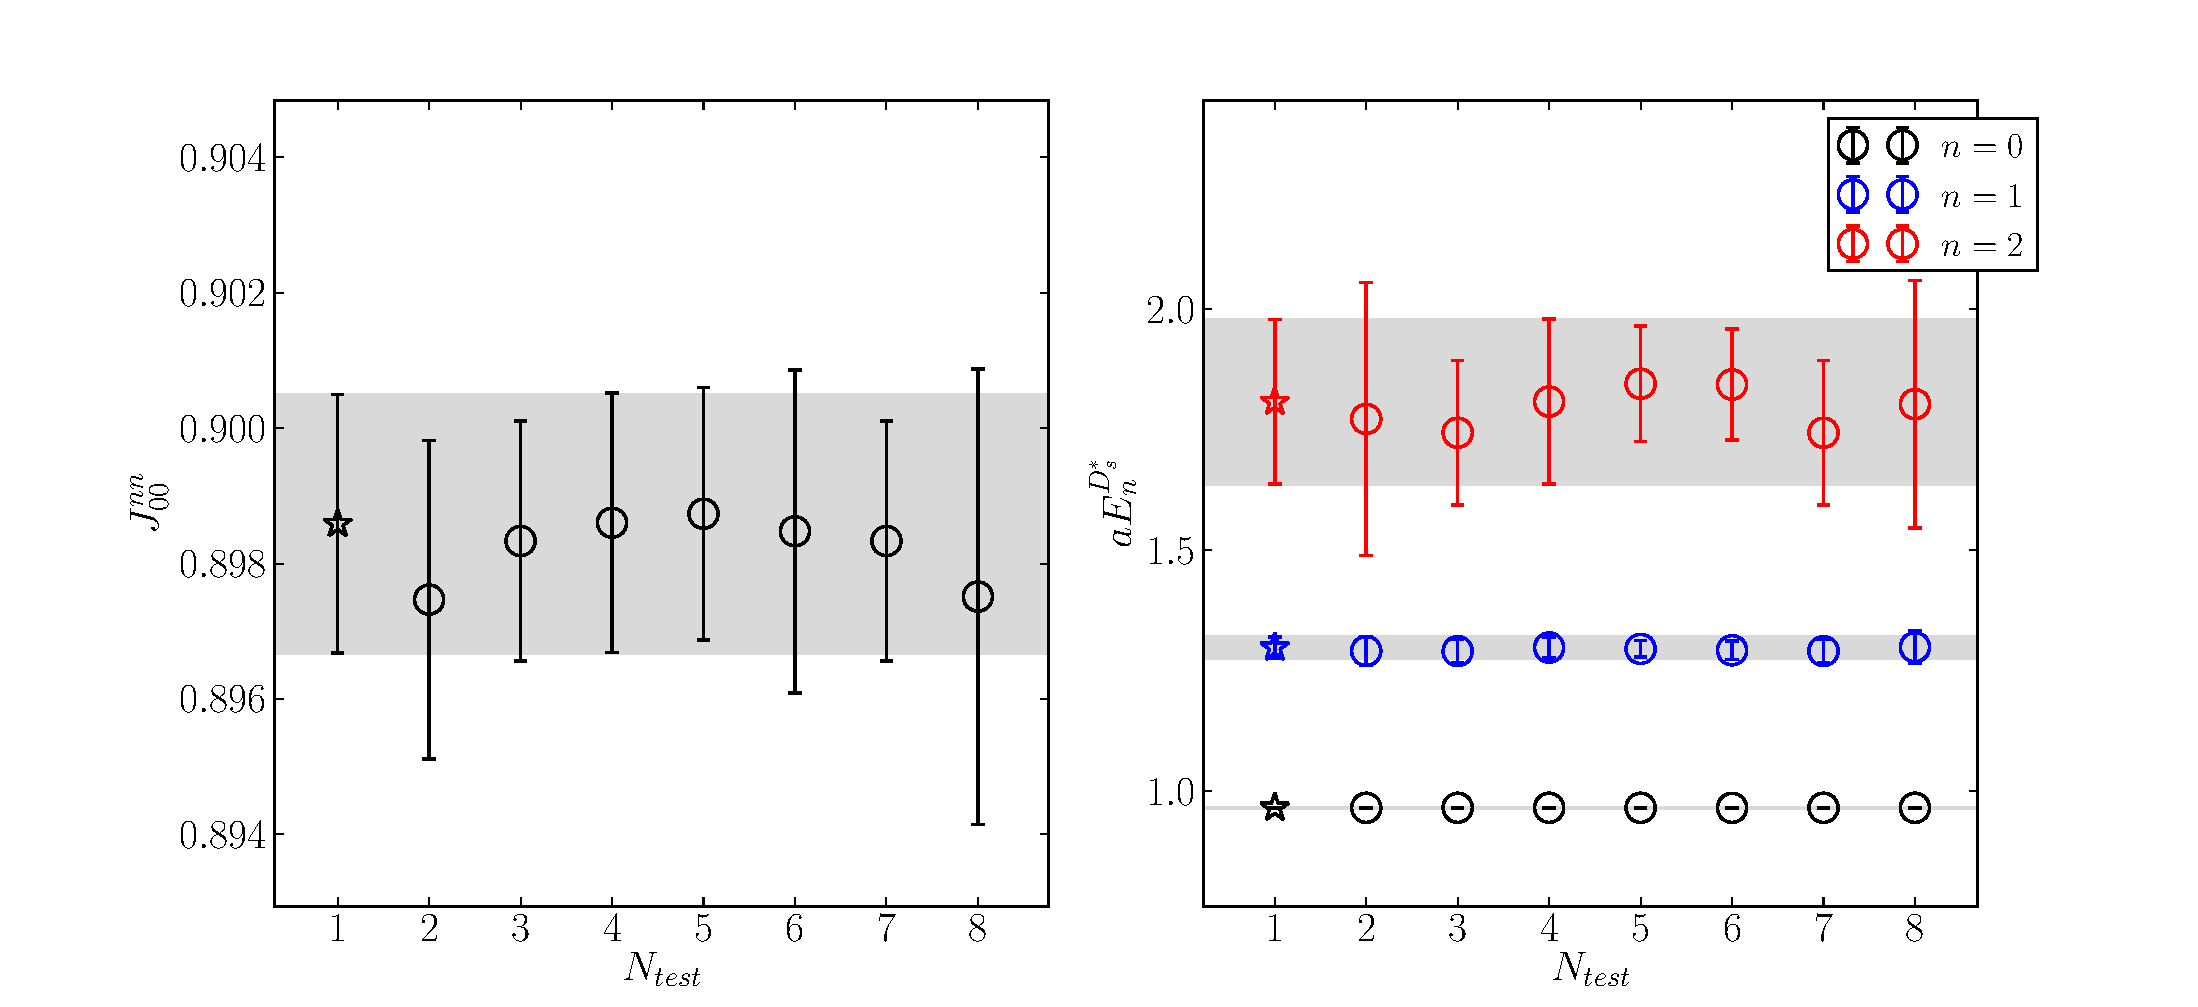
\includegraphics[width=1.1\textwidth]{images/BsDsstar/fittests_fine.pdf}
  \caption{Tests of the correlator fits on the fine ensemble. The left panel shows $J_{00}^{nn}$ at the heavy mass $am_{h0}^{\text{val}}=0.5$. At $N_{\text{test}}=1$ we give the final accepted result. $N_{\text{test}}=2$ gives the results when all priors are broadened by 50\%. $N_{\text{test}}=3$ and $4$ gives the results of setting $N_{\text{exp}}=4$ and $6$ respectively. $N_{\text{test}}=5,6$ gives the results of setting $t_{\text{cut}}=2,4$ respectively for all correlators. $N_{\text{test}}=7$ gives the result without marginalising out the $n=5$ excited state. $N_{\text{test}}=8$ gives the result of moving the SVD cut from $10^{-3}$ to $10^{-2}$. \label{fig:corr_fit_tests}}
  \end{center}
  \vspace{-10pt}
\end{figure}

To ensure that truncating the sum at $N_{\text{exp}}$ is a good approximation to the infinite sum containing all excited states, we only include data with  $t \geq t_{\text{cut}}$ and $t \leq T_{\text{lat}}-t_{\text{cut}}$ in the 2-point case and $t \leq T-t_{\text{cut}}$ in the 3-point case. We can in principle use a different $t_{\text{cut}}$ for every correlation function included in our fit, so must choose a set $\{ t_{\text{cut}}^{c}\}$ (where $c$ labels the correlator).

To ensure the optimal choice for the $\{ t_{\text{cut}}^{c}\}$ set, we employ the \texttt{scikit-optimize} python package \cite{skopt}. The process consists of defining a function $f$ with an input of $\{ t_{\text{cut}}^{c}\}$ and an output of some loss function $f$. Then, the minimum of $f$ with respect to $\{ t_{\text{cut}}^{c}\}$ is found via a Gaussian process. We used the loss function
\begin{align}
  f(\{ t_{\text{cut}}^{c}\}) = - \log \text{GBF} + \theta\left(\chi^2 - N_{\text{dof}}\right) \,\rho\, {\chi^2\over N_{\text{dof}}}.
\end{align}
GBF is the Gaussian Bayes factor corresponding to the comparison between the resulting model of the fit (the fit function with parameters set by the fit), and a random model (the fit function with randomly sampled parameters). The second term gives a strong punishment to fits with $\chi^2/N_{\text{dof}} > 1$. We set $\rho=10^5$, in order to make the second term of comparable size of the first, which for typical fits we attempted had a magnitude of order $10^4$. A couple of more naive choices for $\{ t_{\text{cut}}^{c}\}$ are given in tests $\#5 \,\&\, \#6$.

An appropriate value for the svd cut is found by comparing estimates of eigenvalues of the data's covariance matrix between different bootstrap samples of the data (see Sec. 2.7 of the \texttt{CorrFitter} documentation \cite{CorrFitter}). Typically the smallest eigenvalues are sensitive to taking new bootstrap copies, suggesting they are poorly estimated. A cut is placed such that any poorly estimated eigenvalues are replaced with more conservative (larger) values. The resulting svd cut varies between ensembles since it depends on the quality of the dataset, but are always of order $10^{-3}$.
%% Fig. \ref{fig:svddiagnosis_BsDsstar} illustrates this process on the fine ensemble. 
For example, in fits to the fine ensemble correlators, we set the svd cut to exactly $10^{-3}$. We tested to see if this had any effect by also running the fit with svd cut $10^{-2}$ in test \#8.

%% \begin{figure}[htb!]
%%   \begin{center}
%%   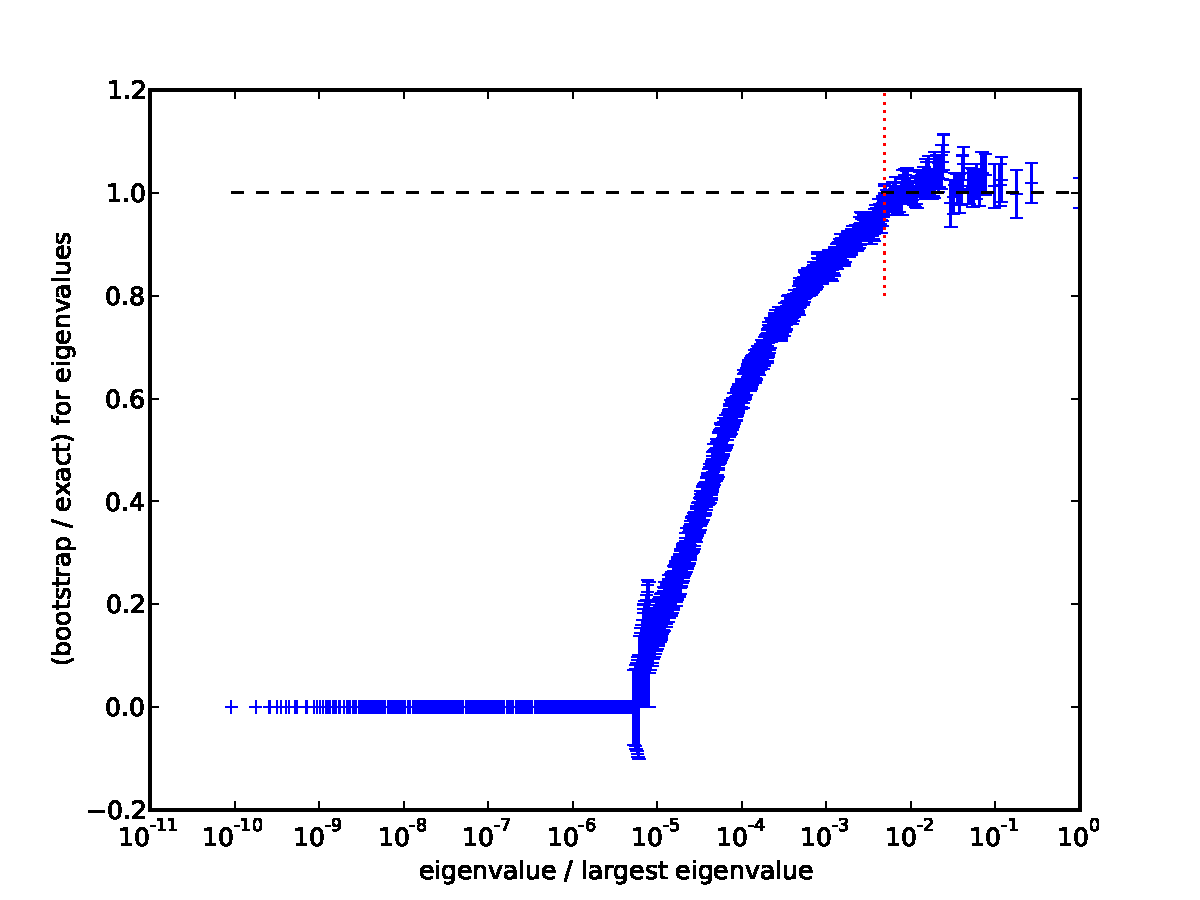
\includegraphics[width=0.8\textwidth]{images/BsDsstar/svddiagnosis_fine.pdf}
%%   \caption{An illustration of the process of deducing an appropriate SVD cut on the fine ensemble. Each point shows the ratio of a covariance matrix eigenvalue, to the same eigenvalue from a bootstrap copy, against the relative size of the eigenvalue. The eigenvalues below the red dotted line are at risk of being underestimated. \label{fig:svddiagnosis_BsDsstar}}
%%   \end{center}
%%   \vspace{-10pt}
%% \end{figure}

We can perform further sanity checks on the fits by plotting certain functions of the 2-point correlators. To obtain useful forms, first one can approximately flush out the oscillating states from correlators by performing a so-called {\it{superaverage}}, $C(t) \to [ C(t) + C(t+a) ]/2$. We perform a doubled and symmetric version of this operator on correlators to obtain
\begin{align}
  C(t) \to \tilde{C}(t) = {1\over 4}( C(t-a) - 2C(t) + C(t+a) ).
  \label{eq:superav2}
\end{align}
We can check the non-oscillating ground-state energy of the correlator by looking at the large-$t$ behaviour of
\begin{align}
  E_{\text{eff}}(t) = \log\left({ \tilde{C}(t)\over \tilde{C}(t-a) }\right).
  \label{eq:effectivemass}
\end{align}
It is straightforward to show from plugging in the fit form for 2-point corrleators (Eq. \eqref{eq:multiexponential}) that in the large $t$ (but $t < T_{\text{lat}}/2$) limit, this should tend towards the ground-state energy for the correlator. One can also construct a similar function for the amplitude:
\begin{align}
  a_{\text{eff}}(t) = \sqrt{{\cosh E_{\text{eff}}(t)-1\over 2} \,\,\tilde{C}(t) e^{E_{\text{eff}}(t)t} }\,.
  \label{eq:effectiveamp}
\end{align}
The $\tilde{C}(t)e^{E_{\text{eff}}(t)t}$ factor would produce the correct amplitude (in the large-$t$ limit) in the absence of superaveraging, and the other factor corrects for the effect of the superaveraging. These functions, for various relevant correlators on the fine ensemble, are plotted in comparison with the full fit results in Fig. \ref{fig:2pt-summary_BsDsstar}.

\begin{figure}[htb!]
  \begin{center}
  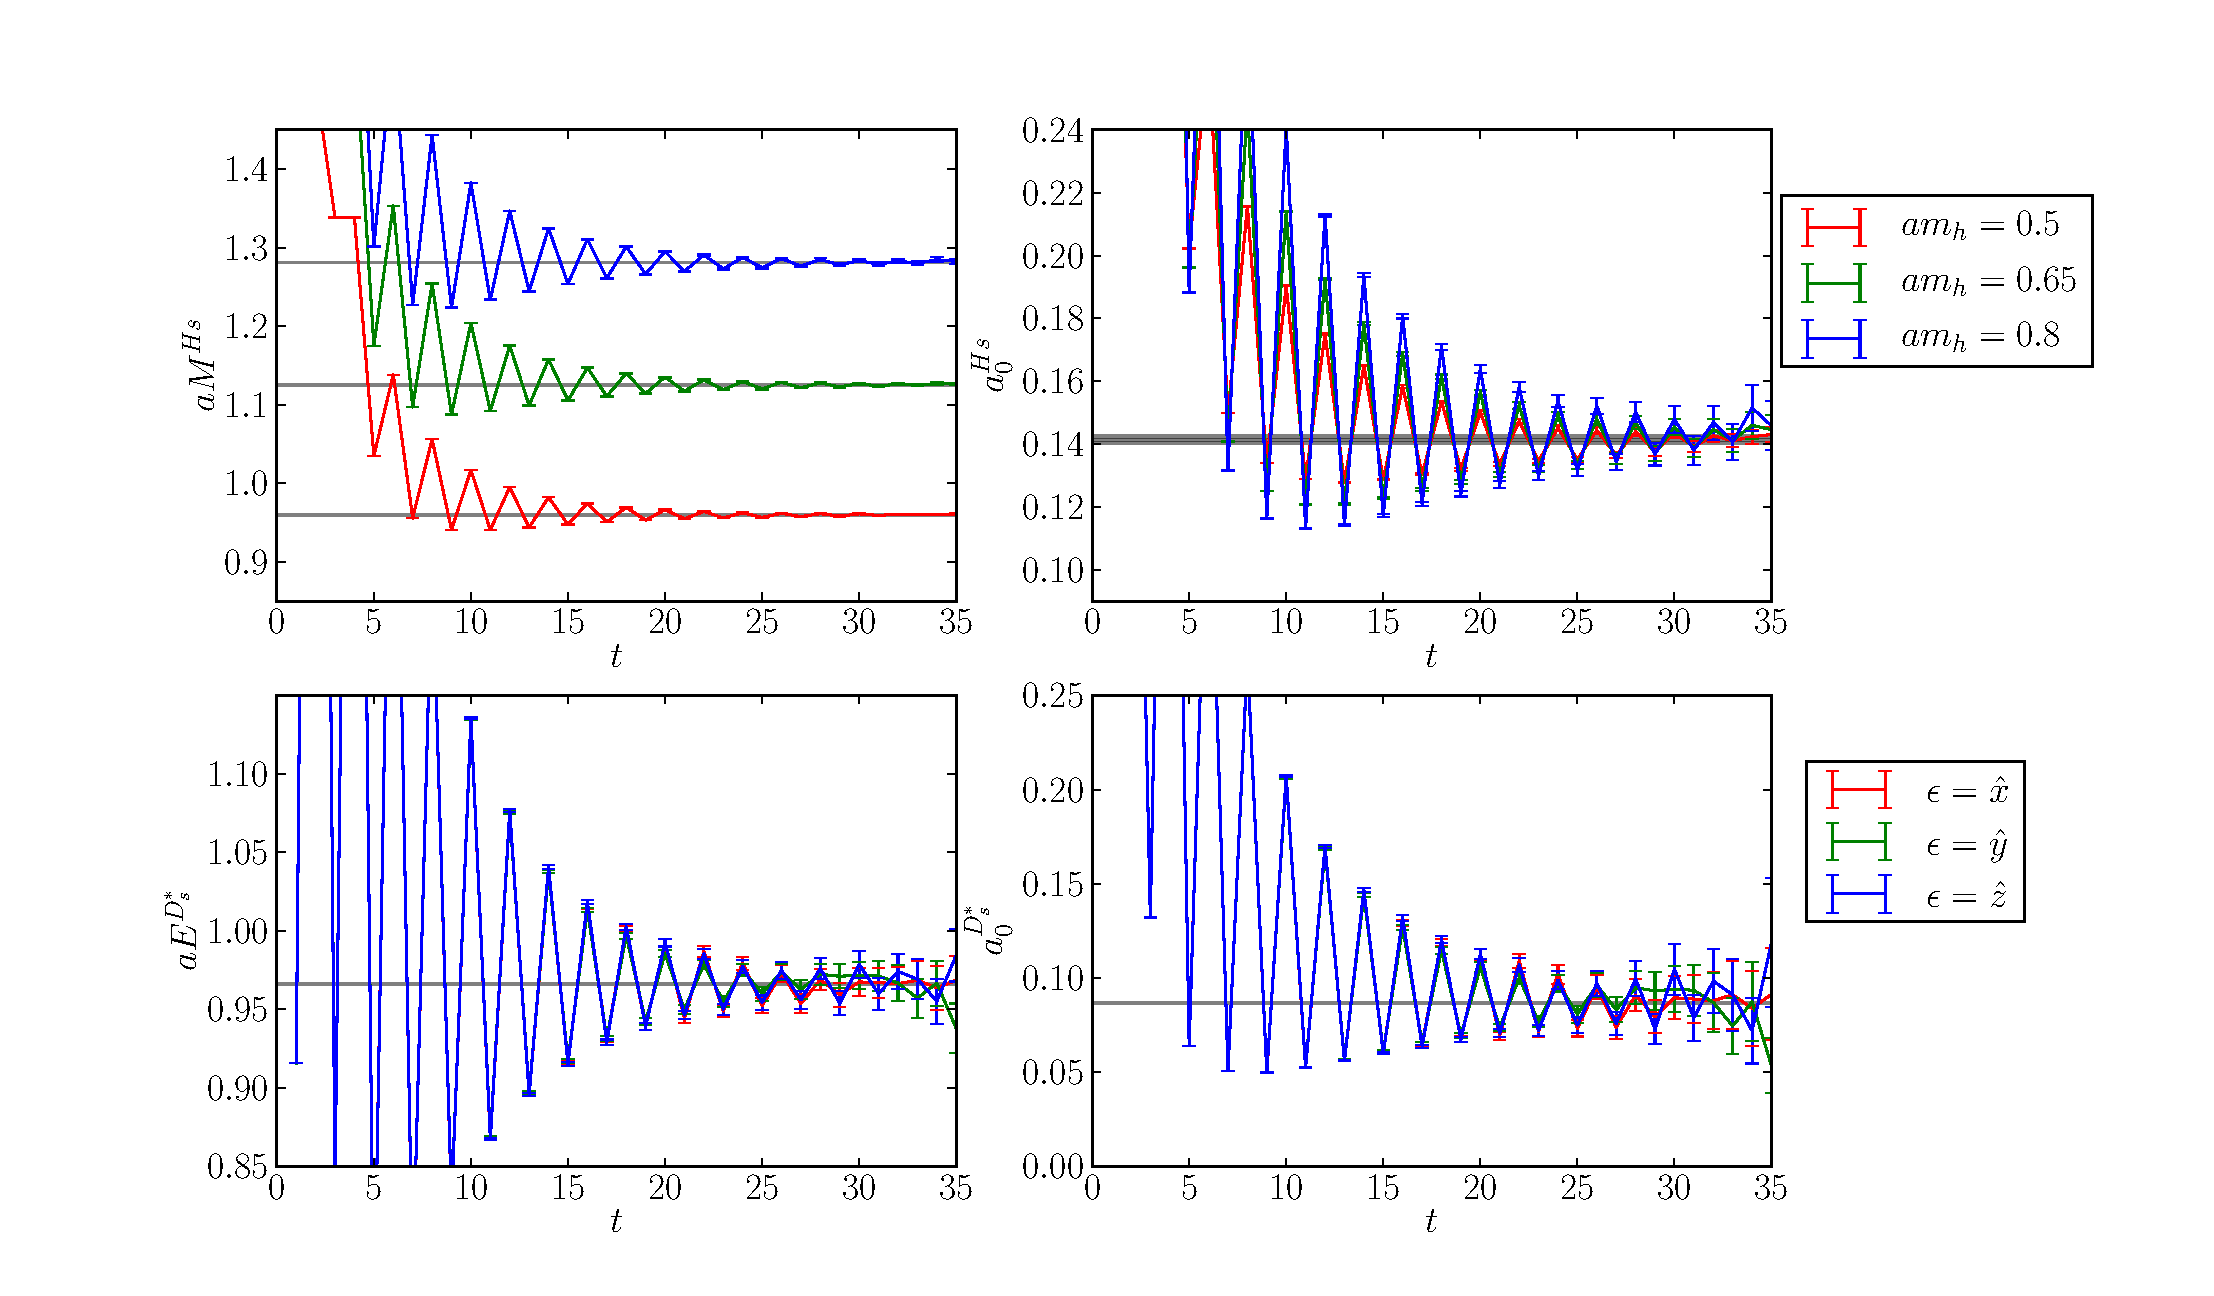
\includegraphics[width=1.1\textwidth]{images/BsDsstar/2ptsummary_fine.pdf}
  \caption{Effective energies and amplitudes for $H_s$ and $D_s^*$ correlators on the fine ensemble. The energies are obtained from Eq. \eqref{eq:effectivemass}, and amplitudes from Eq. \eqref{eq:effectiveamp}. The grey bands give the results of the full multiexponental fit. \label{fig:2pt-summary_BsDsstar}}
  \end{center}
\end{figure}

A similar approach can be applied to the 3-point correlators. The ratio $\tilde{C}_3(t,T)/\tilde{C}_{H_s}(t) \tilde{C}_{D_s^*}(T-t)$ approaches $J_{00}^{nn}/a_0^{H_s}a_0^{D^*_s}$ for $t>>0$ and $t<<T$. This is illustrated in Fig. \ref{eq:3pt-summary_BsDsstar}. From inspecting these figures for 2- and 3-point sanity tests, one can reassure themselves that the fits to the correlators are well behaved.

\begin{figure}[htb!]
  \begin{center}
    \vspace{-10pt}
  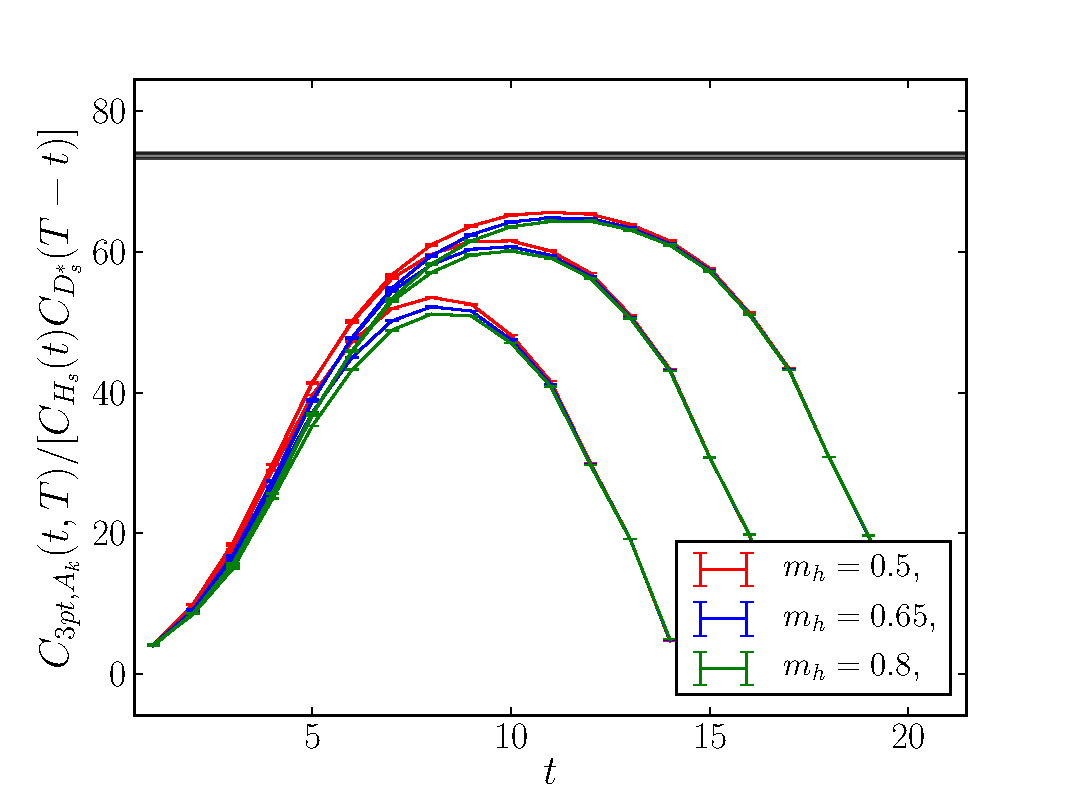
\includegraphics[width=0.8\textwidth]{images/BsDsstar/3ptsummary_fine.pdf}
  \caption{Sanity check for fits to the 3-point correlation functions. This ratio should approach $J_{00}^{nn}$ for $t>>0$ and $t<<T$. The grey band shows the result for $J_{00}^{nn}$ from the full multiexponential fit. If the $T$ values were larger, one can invision the data reaching a plateu at the same height as the grey band. \label{eq:3pt-summary_BsDsstar}}
  \end{center}
  \vspace{-10pt}
\end{figure}

\subsection{Normalization of the Axial Current}

Conserved and partially conserved currents require no renormalization (see Sec. \ref{sec:chiralsymmetry}). However, the staggered conserved axial-vector current is not simply $(\gamma_5\gamma_{\mu}\otimes \gamma_5\gamma_{\mu})$, it is a complicated linear combination of many local and point-split lattice currents. In this study we used only local axial vector currents, this simplifies the lattice calculation but creates the need for our resulting current matrix element to be multiplied by a matching factor $Z_A$ to produce the appropriate continuum current. We found $Z_A$ via a fully non-perturbative method \cite{McNeile:2011ng,Donald:2013pea}.

We leveraged the fact that the staggered local pseudoscalar current $(\gamma_5\otimes \gamma_5)$, multiplied by the sum of masses of quark flavours the current is charged under, is absolutely normalized. We extract from the 2-point $H_c$ and $\hat{H}_c$ correlators the decay amplitudes $\langle \Omega | \bar{c} (\gamma_5\otimes \gamma_5) h | H_c \rangle \equiv \langle \Omega | P | H_c \rangle$ and $\langle \Omega | \bar{c} (\gamma_0\gamma_5 \otimes \gamma_0\gamma_5) h | \hat{H}_c \rangle = \langle \Omega | A_0 | \hat{H}_c \rangle$ from $a_0^{H_c}$ and $a_0^{\hat{H}_c}$. Then, the normalization for $A_0$ (common to that of spacial axial currents $A_k$) $Z_A$, is fixed by demanding that the partially conserved axial current relation holds:
\begin{align}
  (m^{\text{val}}_{h0} + m^{\text{val}}_{c0}) \langle \Omega | P | H_c \rangle|_{\text{lat}} = M_{\hat{H}_c} Z_A \langle \Omega | A_0 | \hat{H}_c \rangle|_{\text{lat}}\,.
  \label{eq:wardBsDsstar}
\end{align}
The $Z_A$ values found on each ensemble and $am^{\text{val}}_{h0}$ are given in Table \ref{tab:norms}.

There is an ambiguity in which mass to use on the right-hand side of Eq. \eqref{eq:wardBsDsstar}, we here use the non-goldstone mass $M_{\hat{H}_c}$, but one could just as well replace this with $M_{H_c}$. Using $M_{H_c}$ here changes $Z_A$ only by discretization effects, the effect on $Z_A$ this causes never exceeds 0.0015 throughout the ensembles and heavy masses. The choice between these two definitions of $Z_A$ has a negligible effect on our final result for $h^s_{A_1}(1)$.

We also remove tree-level mass-dependent discretization effects using a normalization constant derived in \cite{Monahan:2012dq,Bazavov:2017lyh}:
\begin{align}
  \label{eq:Zdisc}
  Z_{\text{disc}} &=\,\sqrt{ \tilde{C}_h \tilde{C}_c }\,, \\
  \nonumber
  &\tilde{C}_q = \cosh am_{q,\text{tree}} \left( 1 - {1+\epsilon_{\text{Naik}}\over 2} \sinh^2 am_{q,\text{tree}} \right)\,,
\end{align}
where $\epsilon_{\text{Naik}}$ is the Naik parameter in the HISQ action and $am_{q,\text{tree}}$ is the tree-level pole mass in HISQ defined in Eq. \eqref{eq:hisq_tree_mass}. The effect of $Z_{\text{disc}}$ is very small, never exceeding $0.2\%$. $Z_{\text{disc}}$ values on each ensemble for each $am^{\text{val}}_{h0}$ are given in Table \ref{tab:norms}.

Combining these normalizations with the lattice current from the 3-point fits, we find a value for the form factor at a given heavy mass and lattice spacing:
\begin{align}
  h_{A_1}^s(1) = {1\over 3} \sum_{k=0}^3 { Z_A Z_{\text{disc}}\langle D_s^*(\hat{k}) | A_k | H_s \rangle |_{\text{lat}}\over 2\sqrt{M_{H_s} M_{D_s^*}} }\,.
  \label{eq:normalizationsBsDsstar}
\end{align}

\begin{table}
\begin{center}
\begin{tabular}{ c c c c }
\hline
Set & $am_h^{\text{val}}$ & $Z_A$& $Z_{\text{disc}}$\\ [0.5ex]
\hline
0 & 0.5 & 1.03178(57) & 0.99819\\ [0.5ex] 
 & 0.65 & 1.03740(58) & 0.99635\\ [0.5ex] 
 & 0.8 & 1.04368(56) & 0.99305\\ [0.5ex] 
\hline
1 & 0.5 & 1.03184(47) & 0.99829\\ [0.5ex] 
 & 0.8 & 1.04390(39) & 0.99315\\ [0.5ex] 
\hline
2 & 0.427 & 1.0141(12) & 0.99931\\ [0.5ex] 
 & 0.525 & 1.0172(12) & 0.99859\\ [0.5ex] 
 & 0.65 & 1.0214(12) & 0.99697\\ [0.5ex] 
 & 0.8 & 1.0275(12) & 0.99367\\ [0.5ex] 
\hline
3 & 0.5 & 1.00896(44) & 0.99889\\ [0.5ex] 
 & 0.65 & 1.01363(49) & 0.99704\\ [0.5ex] 
 & 0.8 & 1.01968(55) & 0.99375\\ [0.5ex] 
\hline
\end{tabular}
\caption{Normalization constants applied to the lattice axial vector current in Eq. \eqref{eq:normalizationsBsDsstar}. $Z_A$ is found from Eq. \eqref{eq:wardBsDsstar} and $Z_{\text{disc}}$ from Eq. \eqref{eq:Zdisc}. \label{tab:norms}}
\end{center}
\end{table}


\subsection{Extrapolation to the Physical Point}
\label{sec:BsDsstar_extrapolation}

We now address the extrapolation of the lattice $h_{A_1}^s(1)$ values to continuum and physical $b$ and $l$ masses. In the process of the extrapolation, we also aim to determine the HQET low energy constants $l^s_{V,A,P}$. This process requires a number of considerations.

\subsubsection{Heavy Mass Dependence}
\label{sec:BsDsstar_heavymass}

Our extrapolation in the $m_h$ direction can be guided by HQET. The HQET expression for $h^s_{A_1}(1)$ (where here we consider both $h$ and $c$ to be heavy quarks in the HQET context) is given by Eq. \eqref{eq:hA1_hqet} from Sec. \ref{sec:Luke}:
\begin{align}
  \label{eq:hqet_hA1}
  h^s_{A_1}(1) &= \eta_A \left( 1 - {l_V\over (2m_c)^2} + {l_A \over 2 m_c m_h} - { l_P \over (2m_h)^2 } \right)  \\ \nonumber &+ \mathcal{O}\left( \, {1\over m_c^n m_h^m}, \, n+m\geq 3 \, \right).
\end{align}
Luke's theorem dictates that this form factor has no $\order{1/m_{h,c}}$ corrections. $\eta_A$ is an ultraviolet matching factor between HQET and QCD, and upsettingly contains (weak) dependence on $m_h$.

\subsubsection{Quark Mass Proxies}
\label{sec:massambiguities}

Attention must be paid to what to input for the masses $m_{h,c}$ in the above expression \eqref{eq:hqet_hA1}. Finding continuum quark masses corresponding to lattice bare masses would be a considerable task. Even if we took this on, what renormalization scheme should the masses belong to? In HQET, the masses that define the power counting should be pole masses \cite{Neubert:1997gu}. Due to renormalons, the definition of a pole mass $m$ also has an ambiguity of order $\Lambda_{\text{QCD}}/m$ \cite{tHooft1979}.

Because of this, we cannot exactly reproduce the HQET expression for $h_{A_1}^s(1)$ \eqref{eq:hqet_hA1} in our fit. We instead test a number of proxies for the quark masses. Since we are not exactly reproducing the HQET expression, our results for $l_{V,A,P}$ are not exact but rather should be interpreted as ballpark estimations.

One possible approach is the following. The quark masses in Eq. \eqref{eq:hqet_hA1} could be related to the meson masses (that we have access to via the correlator fits) using HQET. To see this, first consider the HQET expansion of a heavy-light meson \cite{Bazavov:2018omf}:
\begin{align}
  \label{eq:hqet_mass}
  M_{H_s} = m_{h,\,S} + \bar{\Lambda}_S + { \mu^2_{\pi,\,S} - d_{H^{(*)}} \mu^2_{G,\,S} \over m_{h,\,S}} + \mathcal{O}\left({1\over m_h^2}\right).
\end{align}
where $d_{H^{(*)}} = 1$ for pseudoscalar mesons and $-1/3$ for vectors. $\bar{\Lambda}_S,\mu_{\pi,\,S},\mu_{G,\,S}$ are HQET parameters. $q$ labels the light quark in the meson. As already mentioned, $m_h$ is defined in some renormalization scheme $S$, and since the meson mass $M_{H_q}$ is scheme-independent, the HQET parameters must also take on scheme dependence to cancel the dependence in $m_h$.

A simple rearrangement of the above \eqref{eq:hqet_mass} gives us
\begin{align}
  \label{eq:epsilon_h}
  m_{h,S} &= M_{H_s} - \bar{\Lambda}_S - { \mu^2_{\pi,\,S} - d_{H^{(*)}} \mu^2_{G,\,S} \over M_{H_s} - \bar{\Lambda}_S} + \mathcal{O}\left({1\over m_h^2}\right)\,, \\ \nonumber
  & \equiv {1\over\varepsilon_{h,\,S}} + \mathcal{O}\left({1\over m_h^2}\right)\,.
\end{align}

For two heavy-light mesons, for example $M_{H_s},M_{D_s^*}$, one can show (recognising that $\varepsilon_{h}\sim \mathcal{O}(1/m_h)$)
\begin{align}
  {1\over m_{h,\,S} m_{c,\,S}} = \varepsilon_{h,\,S}\varepsilon_{c,\,S} + \mathcal{O}\left( \, {1\over m_c^n m_h^m}, \, n+m\geq 3 \, \right)\,.
\end{align}
Since we are aiming to find the low energy constants in the context of HQET at order below $\mathcal{O}( 1/ m_c^n m_h^m, n+m\geq 3 )$, we can safely replace the quark masses $m_c,m_h$ in \eqref{eq:hqet_hA1} with $\varepsilon_{h/c}^{-1}$.

For our calculation, we used HQET parameters calculated in \cite{Bazavov:2018omf} in the minimal renormalon-subtraction scheme: $\bar{\Lambda}_{\text{MRS}} = 0.552(30)\text{GeV} \,,\, \mu^2_{\pi,\text{MRS}} = 0.06(22)\text{GeV}^2 \,, \, \mu^2_{G,\text{MRS}} = 0.38(1)\text{GeV}^2$. We are free to arbitrarily choose this choice of scheme, since the resulting ambiguety in the masses, $\Lambda_{\text{QCD}}/m_{h,c}$, are absorbed into higher orders in the HQET expansion.

Unfortunately, the quark mass dependence in $\eta_A$ prevents this approach from resulting in exactly the correct $l_{V,A,P}$ values. $\eta_A$ contains ratios $m_c/m_h$ and logs of $m_c/m_h$, that cannot simply be redefined in this way such that ambiguities are pushed into higher orders of $1/m_{h,c}$.

We also implement the fit with more simple proxies for $m_{h,c}$. We tried replacing $m_{h,c}$ with $M_{H_s,D^*_s}$ or $M_{\eta_{h,c}}/2$. We find the results of the extrapolation are very insensitive to the choice of proxy (see Fig. \ref{fig:fittests_hA1}). Therefore in the end, we take our final fit function using the simplest choice of replacing $m_{h,c}$ with $M_{\eta_{h,c}}/2$. This means we have not inserted any ambiguety due to renormalization scheme choice.

%% One would expect that performing a fit using these scheme-dependent parameters will produce outputs $l^s_{V,A,P}$ containing a scheme ambiguity. However, renormalon ambiguities in a pole mass $m$ are of order $\mathcal{O}(1/m)$. The ambiguity in the low-energy constants will, in fact, be absorbed by the next order in $1/m$, which we can safely ignore. Hence we can drop the renormalization scheme subscripts.

\subsubsection{Implementation of $\eta_A$}

$\eta_A$ accounts for matching between HQET and QCD, and has been computed to 2-loop: $\eta_A = 0.960(7)$ \cite{PhysRevLett.76.4124}. It is dependent on $m_{h,c}$, so one may worry that, if we are going to use this expression for the extrapolation in $m_h$, we must account for the $m_h$ dependence in $\eta_A$. However this dependence is weak in the region of $m_h$ we are interested in ($m_c \leq m_h \leq m_b$). This can be seen by examining how the 1-loop expression for $\eta_A$ varies with $m_h$ \cite{CLOSE1984209}:
\begin{align}
  \eta_A(m_h) = 1 - {\alpha_s \over \pi} \left( {m_h+m_c\over m_h-m_c} \ln\left({m_c\over m_h}\right) + {8\over 3} \right).
  \label{eq:etaA}
\end{align}
Fig. \ref{fig:etaAV} shows the variation of $\eta_A$ throughout this range, the value changes by around 1\%. The two-loop correction is an order of magnitude smaller than this \cite{PhysRevLett.76.4124}.

\begin{figure}[htb!]
  \begin{center}
  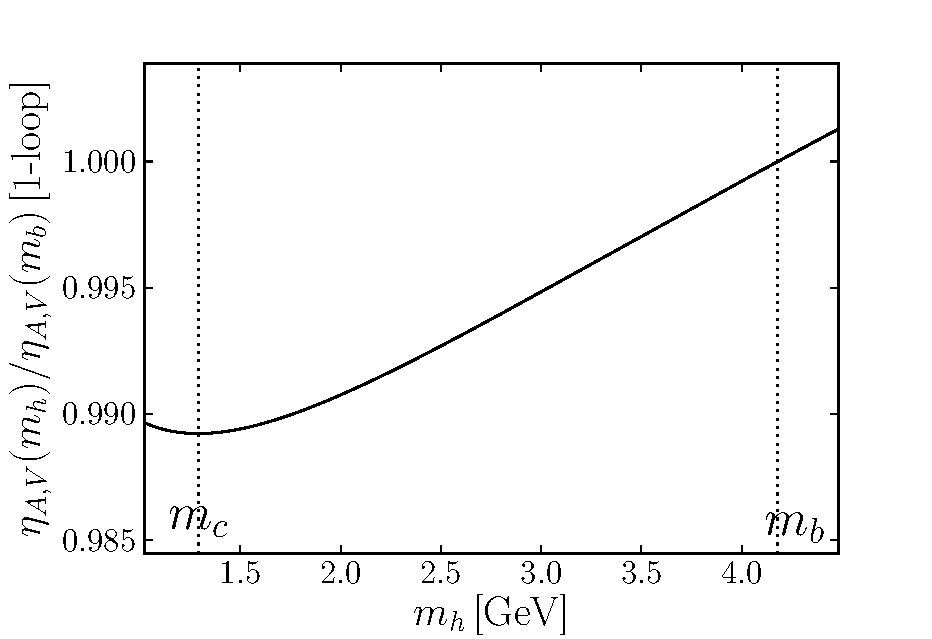
\includegraphics[width=0.6\textwidth]{images/BsDsstar/etaAV.pdf}
  \caption{The variation of the 1-loop expression for $\eta_{A}$ \& $\eta_V$ throughout the $m_c \leq m_h \leq m_b$ range. \label{fig:etaAV}}
  \end{center}
  \vspace{-10pt}
\end{figure}

We cannot consistently include $\eta_A$ in our fit function since we do not have access to the pole $m_{h,c}$ masses. We ran the extrapolation using a number of reasonable approaches to estimating the $\eta_A$ behaviour and found that the final result was very insensitive to our choice of approach. We implemented the extrapolation with
\begin{itemize}
\item
  $\eta_A=1$,
\item
  $\eta_A = $1-loop expression with $m_c/m_h$ replaced with $M_{\eta_c}/M_{\eta_h}$,
\item
  $\eta_A = 1 + \rho \log(M_{\eta_c}/M_{\eta_h})$, where $\rho$ is a fit parameter with prior distribution $0\pm 1$.
\end{itemize}

The final result was stable upon varying these choices (see Fig. \ref{fig:fittests_hA1}). The last bullet point, for testing to see if logarithms of $m_h$ can be resolved in the data, resulted in a $\rho$ consistent with zero and a decrease of the Bayes factor for the fit by a factor of 25. Clearly, the lattice data cannot resolve logarithms in $m_h$.

We choose $\eta_A=1$ for simplicity. The $l_{V,A,P}$ results however are sensitive to the $\eta_A$ implementation, since not properly accounting for the $m_h$ dependence in $\eta_A$ can lead to that variance in $m_h$ being absorbed into $l_{V,A,P}$. This is another reason to take our $l_{V,A,P}$ results as estimates rather than determinations.

The fit form we used for the full extrapolation of $h_{A_1}^s(1)$ is
\begin{align}
  h^s_{A_1}(1)|_{\text{fit}} &= 1 - \left({1\over M_{\eta_c}}\right)^2 l_V + {2\over M_{\eta_h}M_{\eta_c}} l_A- \left({1\over M_{\eta_h}}\right)^2 l_P  \nonumber \\ &+ \mathcal{N}_{\text{disc}} + \mathcal{N}_{\text{mistuning}}.
  \label{eq:fitform_BsDsstar}
\end{align}

$\mathcal{N}_{\text{disc}}$ and $\mathcal{N}_{\text{mistuning}}$ are nuisance parameters to account for discretization and mass mistuning effects, defined in the following subsections. $l_{V,A,P}$ are taken here as fit parameters with prior distributions $0\pm 1 $GeV$^2$.

\subsubsection{Discretization Effects}

Discretization effects in the data are accounted for by including (following the methodology of \cite{McNeile:2012qf}):
\begin{align}
    \label{eq:fitfun_hA1}
  \mathcal{N}_{\text{disc}} = &\sum_{i=0,\,j+k\neq 0}^{2,2,2} d_{ijk} \left({2\Lambda_{\text{QCD}}\over M_{\eta_h} }\right)^{i} \left({ am^{\text{val}}_{h0} \over \pi }\right)^{2j} \left({ am^{\text{val}}_{c0} \over \pi }\right)^{2k}.
\end{align}
$d_{ijk}$ are fit parameters with prior distributions $0\pm 1$. We account here for discretization effects from the two largest scales in the system; the heavy and charm masses. All discretization effects are of even order by construction of the HISQ action.

We tried including extra terms of size $(a\Lqcd)^2$,$(am^{\text{val}}_{s0})^2$,$(am^{\text{val}}_{l0})^2$, but the data could not resolve effects of that size, so it made no difference to the fit. We also tested the effects of increasing the number of terms in each sum (see Fig. \ref{fig:fittests_hA1}), but the final result remained unchanged.

\subsubsection{Mass Mistunings}

Any possible mistuning of the charm mass is automatically accounted for in HQET part of the fit function \eqref{eq:fitform_BsDsstar}. To obtain the final result we set $M_{\eta_c}$ to the physical value given in the PDG \cite{PhysRevD.98.030001}, hence any charm mistuning is removed.

The strange and light mistunings are accounted for using a formalism introduced in \cite{Chakraborty:2014aca}. To deal with possible (valence and sea) strange mistuing, we define the terms $\delta^{(\text{val})}_s = m^{(\text{val})}_{s0}- m_s^{\text{tuned}}$, where $m_s^{\text{tuned}}$ is defined by
\begin{align}
  m_s^{\text{tuned}} = m_{s0} \left({ M^{\text{phys}}_{\eta_s} \over M_{\eta_s} }\right)^2.
\end{align}
$M_{\eta_s}^{\text{phys}}$ is determined in lattice simulations from the masses of the pion and kaon \cite{Dowdall:2013rya}.

We similarly account for (sea) light quark mistuning by defining $\delta_l = m_{l0} - m_l^{\text{tuned}}$. We can find $m_l^{\text{tuned}}$ from $m_s^{\text{tuned}}$, by leveraging the fact that the ratio of quark masses is regularization independent and was calculated in \cite{Bazavov:2017lyh} to be
\begin{align}
  \left.\frac{m_s}{m_l}\right\rvert_{\textrm{phys}} = 27.18(10)\,.
\end{align}
We set $m_l^{\text{tuned}}$ to $m_s^{\text{tuned}}$ divided by this ratio.

Chiral perturbation theory dictates that perturbations in quark masses cause linear contributions to the form factor. Hence the full term we include to account for mistuning is given by
\begin{align}
  \mathcal{N}_{\text{mistuning}} = {c^{\text{val}}_s \delta^{\text{val}}_s + c_s \delta_s + c_l \delta_l \over 10 m_s^{\text{tuned}}}\,,
  \label{eq:mistuning_BsDsstar}
\end{align}
where $c_s^{\text{val}}$, $c_s$ and $c_s$ are fit parameters with prior distributions $0\pm 1$. We divide all terms by $m_s^{\text{tuned}}$ to absorb any running of the quark masses in $\delta_{l,s}^{(\text{val})}$ with the cutoff, that varies between ensembles. The factor of 10 in the denominator is to bring this term close in magnitude to the chiral perturbation theory contributions that it represents. We neglect $\delta^{(\text{val})\,2}_{s,l}$ contributions since these are an order of magnitude smaller and are not resolved by the data.

\subsubsection{Negligable Effects}

The finite volume effects in our lattice results are negligible. Since the lightest valence quarks in our simulation are $s$ quarks, the lightest particles that can arise from loop diagrams in the decay are Kaons. In appendix F of \cite{Harrison:2017fmw}, the HMS$\chi$PT finite volume effect on the fine-physical ensemble, as a function of the lightest meson appearing in loops, was found (from the formulas derived in \cite{Laiho:2005ue}). At the Kaon mass, the finite volume effect is many orders of magnitude smaller than any of our other sources of error. 

In our simulation we set $m_u=m_d\equiv m_l$, our results do not account for the difference $m_d-m_u$. We tested for any possible influence this has on our fit, by moving the $m_l^{\text{tuned}}$ value up and down by the PDG value for $m_d-m_u$ \cite{PhysRevD.98.030001}. The effect was negligible in comparison to the other sources of error.

Since we take the physical result at $M_{\eta_h}=M_{\eta_b}$, the uncertainty in $M_{\eta_b}$ will contribute an uncertainty in the final result. We use the PDG result for $M_{\eta_h}$ \cite{PhysRevD.98.030001}. However, $\bar{b}-b$ annihilation and electroweak corrections make this somewhat different to the appropriate value on the lattice. We estimate the corresponding uncertainty in $M_{\eta_b}$ to be no greater than $\pm10$MeV. To see how this changes the result of the extrapolation, we varied $M_{\eta_b}$ up and down by 10MeV and studied how our final result for $h_{A_1}^s(1)$ changes. The change is less than $10^{-5}$, which is negligible in comparison to our other errors.

\section{Results}
\label{sec:results_BsDsstar}

\subsection{$h^s_{A_1}(1)$}

The values extracted from correlation function fits for $h^s_{A_1}(1)$, along with quantities required for its extrapolation to the physical point, are given in Tables \ref{tab:results_BsDsstar} and \ref{tab:results2_BsDsstar}.

\begin{table}
\begin{center}
\begin{tabular}{ c c c c c }
\hline
Set & $am_h^{\text{val}}$ & $h^s_{A_1}(1)$& $aM_{H_s}$& $aM_{D^*_s}$\\ [0.5ex]
\hline
0 & 0.5 & 0.9255(20) & 0.95972(12) & 0.96616(44)\\ [0.5ex] 
 & 0.65 & 0.9321(22) & 1.12511(16) & \\ [0.5ex] 
 & 0.8 & 0.9434(24) & 1.28128(21) & \\ [0.5ex] 
\hline
1 & 0.5 & 0.9231(21) & 0.95462(12) & 0.93976(42)\\ [0.5ex] 
 & 0.8 & 0.9402(27) & 1.27577(22) & \\ [0.5ex] 
\hline
2 & 0.427 & 0.9107(46) & 0.77453(24) & 0.63589(49)\\ [0.5ex] 
 & 0.525 & 0.9165(49) & 0.88487(31) & \\ [0.5ex] 
 & 0.65 & 0.9246(65) & 1.02008(39) & \\ [0.5ex] 
 & 0.8 & 0.9394(66) & 1.17487(54) & \\ [0.5ex] 
\hline
3 & 0.5 & 0.9143(51) & 0.80245(24) & 0.47164(39)\\ [0.5ex] 
 & 0.65 & 0.9273(62) & 0.96386(33) & \\ [0.5ex] 
 & 0.8 & 0.9422(72) & 1.11787(43) & \\ [0.5ex] 
\hline
\end{tabular}
\caption{Values extracted from correlation function fits for $h^s_{A_1}(1)$, along with masses of the two mesons on either end of the transition. $h^s_{A_1}(1)$ values are found from Eq. \eqref{eq:normalizationsBsDsstar}. \label{tab:results_BsDsstar}}
\end{center}
\end{table}

\begin{table}
\begin{center}
\begin{tabular}{ c c c c c c c }
\hline
Set & $am_h^{\text{val}}$ & $aM_{H_c}$& $af_{H_c}$& $aM_{\eta_h}$& $aM_{\eta_c}$& $aM_{\eta_s}$\\ [0.5ex]
\hline
0 & 0.5 & 1.419515(41) & 0.186299(70) & 1.471675(38) & 1.367014(40) & 0.313886(75)\\ [0.5ex] 
 & 0.65 & 1.573302(40) & 0.197220(77) & 1.775155(34) & & \\ [0.5ex] 
 & 0.8 & 1.721226(39) & 0.207068(78) & 2.064153(30) & &\\ [0.5ex] 
\hline
1 & 0.5 & 1.400034(28) & 0.183472(62) & 1.470095(25) & 1.329291(27) & 0.304826(52)\\ [0.5ex] 
 & 0.8 & 1.702456(23) & 0.203407(45) & 2.062957(19) & & \\ [0.5ex] 
\hline
2 & 0.427 & 1.067224(46) & 0.126564(70) & 1.233585(41) & 0.896806(48) & 0.207073(96)\\ [0.5ex] 
 & 0.525 & 1.172556(46) & 0.130182(72) & 1.439515(37) & & \\ [0.5ex] 
 & 0.65 & 1.303144(46) & 0.133684(75) & 1.693895(33) & & \\ [0.5ex] 
 & 0.8 & 1.454205(46) & 0.137277(79) & 1.987540(30) & & \\ [0.5ex] 
\hline
3 & 0.5 & 1.011660(32) & 0.098970(52) & 1.342639(65) & 0.666586(89) & 0.15412(17)\\ [0.5ex] 
 & 0.65 & 1.169761(34) & 0.100531(60) & 1.650180(56) & & \\ [0.5ex] 
 & 0.8 & 1.321647(37) & 0.101714(70) & 1.945698(48) & & \\ [0.5ex] 
\hline
\end{tabular}
\caption{Values extracted from correlation function fits. $f_{H_c}$  is the $H_c$ decay constant derived from Eq. \eqref{eq:decayconstant_pseudoscalar}. \label{tab:results2_BsDsstar} }
\end{center}
\end{table}


%% \begin{table}
%%   \begin{center}
%%     \begin{tabular}{ c c c c c }
%%       \hline
%%       Set & $am_h^{\text{val}}$ & $h^s_{A_1}(1)$& $aM_{H_s}$& $aM_{D^*_s}$ \\ [0.5ex]
%%       \hline
%%       0 & 0.5 & 0.9255(20) & 0.95972(12) & 0.96616(44)\\ [0.5ex]
%%       & 0.65 & 0.9321(22) & 1.12511(16) & \\ [0.5ex]
%%       & 0.8 & 0.9434(24) & 1.28128(21) & \\ [0.5ex]
%%       \hline
%%       1 & 0.5 & 0.9231(21) & 0.95462(12) & 0.93976(42)\\ [0.5ex]
%%       & 0.8 & 0.9402(27) & 1.27577(22) & \\ [0.5ex]
%%       \hline
%%       2 & 0.427 & 0.9107(46) & 0.77453(24) & 0.63589(49)\\ [0.5ex]
%%       & 0.525 & 0.9165(49) & 0.88487(31) & \\ [0.5ex]
%%       & 0.65 & 0.9246(65) & 1.02008(39) & \\ [0.5ex]
%%       & 0.8 & 0.9394(66) & 1.17487(54) & \\ [0.5ex]
%%       \hline
%%       3 & 0.5 & 0.9143(51) & 0.80245(24) & 0.47164(39)\\ [0.5ex]
%%       & 0.65 & 0.9273(62) & 0.96386(33) & \\ [0.5ex]
%%       & 0.8 & 0.9422(72) & 1.11787(43) & \\ [0.5ex]
%%       \hline
%%     \end{tabular}
%%     \caption{Values extracted from correlation function fits for $h^s_{A_1}(1)$, along with quantities required for its extrapolation to the physical point. $h^s_{A_1}(1)$ values are found from eq. \eqref{eq:normalizationsBsDsstar}. $f_{H_c}$  is the $H_c$ decay constant derived from the $H_c$ correlators and Eq. \eqref{eq:decayconstant_pseudoscalar}.  \label{tab:results} }
%%   \end{center}
%% \end{table}


%% \begin{table}
%%   \begin{center}
%%     \begin{tabular}{ c c c c c c c }
%%       \hline
%%       Set & $am_h^{\text{val}}$ & $aM_{H_c}$& $af_{H_c}$& $aM_{\eta_h}$& $aM_{\eta_c}$& $aM_{\eta_s}$\\ [0.5ex]
%%       \hline
%%       0 & 0.5 & 1.419515(41) & 0.186299(70) & 1.471675(38) & 1.367014(40) & 0.313886(75)\\ [0.5ex]
%%       & 0.65 & 1.573302(40) & 0.197220(77) & 1.775155(34) & & \\ [0.5ex]
%%       & 0.8 & 1.721226(39) & 0.207068(78) & 2.064153(30) & & \\ [0.5ex]
%%       \hline
%%       1 & 0.5 & 1.400034(28) & 0.183472(62) & 1.470095(25) & 1.329291(27) & 0.304826(52)\\ [0.5ex]
%%       & 0.8 & 1.702456(23) & 0.203407(45) & 2.062957(19) & & \\ [0.5ex]
%%       \hline
%%       2 & 0.427 & 1.067224(46) & 0.126564(70) & 1.233585(41) & 0.896806(48) & 0.207073(96)\\ [0.5ex]
%%       & 0.525 & 1.172556(46) & 0.130182(72) & 1.439515(37) & & \\ [0.5ex]
%%       & 0.65 & 1.303144(46) & 0.133684(75) & 1.693895(33) & & \\ [0.5ex]
%%       & 0.8 & 1.454205(46) & 0.137277(79) & 1.987540(30) & & \\ [0.5ex]
%%       \hline
%%       3 & 0.5 & 1.011660(32) & 0.098970(52) & 1.342639(65) & 0.666586(89) & 0.15412(17)\\ [0.5ex]
%%       & 0.65 & 1.169761(34) & 0.100531(60) & 1.650180(56) & & \\ [0.5ex]
%%       & 0.8 & 1.321647(37) & 0.101714(70) & 1.945698(48) & & \\ [0.5ex]
%%       \hline
%%     \end{tabular}
%%     \caption{Values extracted from correlation function fits for $h^s_{A_1}(1)$, along with quantities required for its extrapolation to the physical point. $h^s_{A_1}(1)$ values are found from eq. \eqref{eq:normalizationsBsDsstar}. $f_{H_c}$  is the $H_c$ decay constant derived from eq. \eqref{eq:decayconstant_pseudoscalar}. \label{tab:results2} }
%%   \end{center}
%% \end{table}

The results of the extrapolation through heavy mass of $h_{A_1}^s(1)$ is depicted in Fig. \ref{fig:hA1_vsmetah}. By evaluating our fit form \eqref{eq:fitform_BsDsstar} at $a=0$, $M_{\eta_{h,c}}=M_{\eta_{h,c}}^{\text{phys}}$ and $\delta_{s,l}^{(\text{sea})}=0$, we reach our final, fully non-perturbative result for the $B_s\to D_s^*$ form factor at zero recoil:
\begin{align}
  \mathcal{F}^{B_s\to D_s^*}(1) = h^s_{A_1}(1) = 0.9020(96)_{\text{stat}}(90)_{\text{sys}}\,.
  \label{eq:finalresult_hA1}
\end{align}
Adding the statistical and systematic errors in quadrature, we find a total fractional error of $1.45\%$. The error budget for this result is given in Table \ref{tab:errorbudget_BsDsstar}. The continuum/quark mass extrapolation had a goodness of fit of $\chi^2/N_{\text{dof}} = 0.16$ (for $N_{\text{dof}}=12$).

\begin{figure}[htb!]
  \begin{center}
  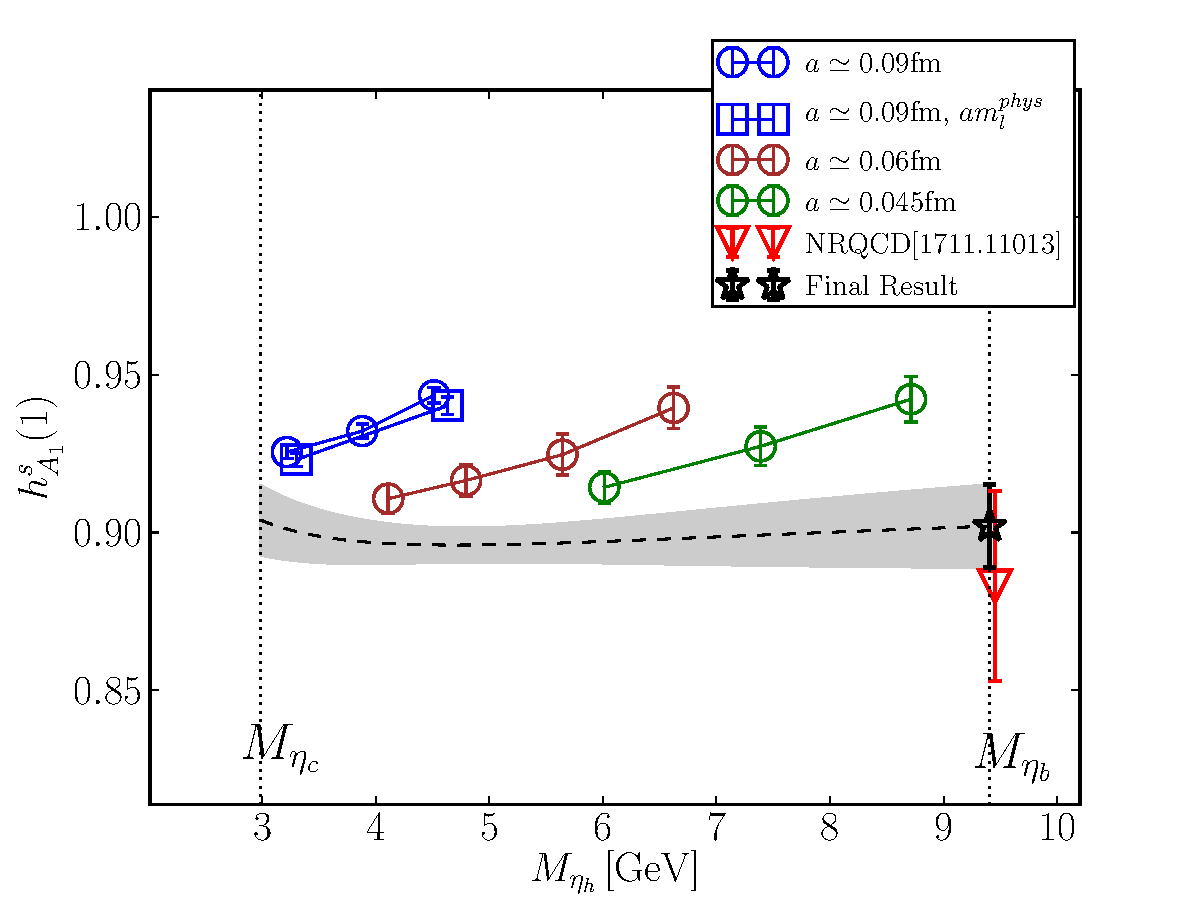
\includegraphics[width=0.90\textwidth]{images/BsDsstar/hA1_vsmh.pdf}
  \caption{ $h_{A_1}^s(1)$ against $M_{\eta_h}$ (a proxy for the heavy quark mass). The grey band shows the result of the extrapolation at $a=0$ and physical $l$,$s$ and $c$ masses. Sets listed in the legend follow the order of sets in Table \ref{tab:BsDsensembles}. The red point represents a determination of the same quantity from a previous study using the NRQCD action for the $b$ \cite{Harrison:2017fmw}. \label{fig:hA1_vsmetah}}
  \end{center}
\end{figure}

\begin{table}
  \begin{center}
    \begin{tabular}{c c}
      \hline
      Source & \% Fractional Error \\ [0.5ex]
      \hline
      Statistics \& $Z_A$ & 1.06  \\ [1ex]
      $a\to 0$ & 0.73  \\ [1ex]
      $m_h \to m_b$, $c$-mistuning & 0.69 \\ [1ex]
      $l$ and $s$  mistuning & 0.20  \\ [1ex]
      \hline
      Total & 1.45 \\ [1ex]
      \hline
    \end{tabular}
  \end{center}
  \caption{Error budget for $h^s_{A_1}(1)$. \label{tab:errorbudget_BsDsstar}}
\end{table}

We include in Fig. \ref{fig:hA1_vsmetah} a determination from the only other lattice calculation of this quantity \cite{Harrison:2017fmw}. They report a value of $h_{A_1}^s(1) = 0.883(12)_{\text{stat}}(28)_{\text{sys}}$. Our two studies, containing independent systematic uncertainties, are in agreement. Their study used the same gluon ensembles, with HISQ $s$ and $c$ valence quarks, and an NRQCD $b$ quark. Using NRQCD meant they could perform their simulation directly at the physical $b$ mass. However, the matching of lattice NRQCD-HISQ currents to continuum QCD causes their dominant error. Their result contains errors associated with the truncation of the NRQCD-HISQ current, of sizes $\order{\alpha_s^2},\order{\alpha_s \Lqcd/m_b}$ and $\order{(\Lqcd/m_b)^2}$. Adding these corrections in quadrature we find a 2.8\% error, while their total error is reported as 2.9\%. Our result is much more precise since it does not suffer from these large matching errors.

\subsection{Implications for $B\to D^*$}

Chiral symmetry implies that the $B_s\to D_s^*$ form factor should be very close to the equivalent $B\to D^*$ form factor \cite{Laiho:2005ue}. This was found to be the case in previous studies (e.g. \cite{Harrison:2017fmw}). 

As an additional test of this claim, we obtained lattice data for $h_{A_1}(1)$ on the fine ensemble, for comparison with the $h_{A_1}^s(1)$ data within our formalism. This involved an identical process to that of obtaining $h_{A_1}^s(1)$, except with the strange valence quark replaced with a valence quark of a mass equal to $am_{l0}$, the sea light quark mass.

The $h_{A_1}(1)$ data is shown in comparison to the $h_{A_1}^s(1)$ data in Fig. \ref{fig:BDstar_BsDsstar}. Errors are statistical. The error on $h_{A_1}(1)$ is much larger due to the presence of the valence light quark. There is no statistically significant difference between $h_{A_1}(1)$ and $h_{A_1}^s(1)$ here.

\begin{figure}[htb!]
  \begin{center}
  \hspace{-10pt}
  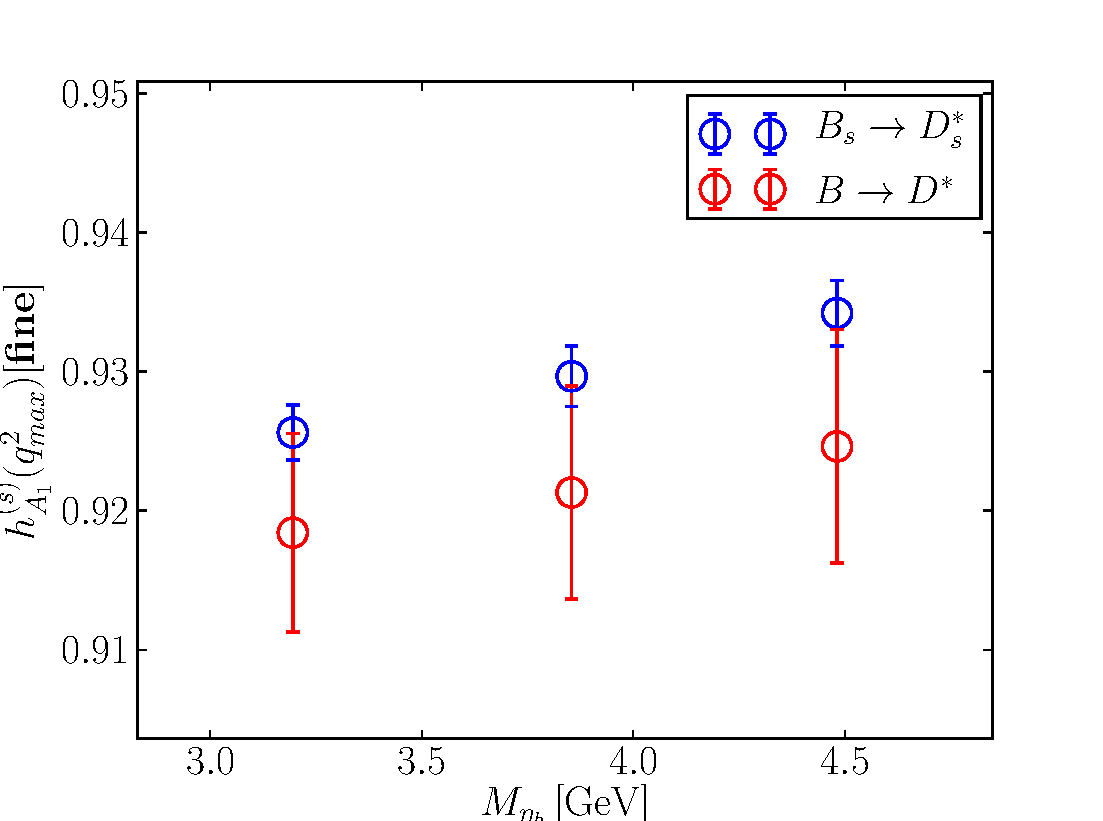
\includegraphics[width=0.7\textwidth]{images/BsDsstar/BD_BsDs.pdf}
  \caption{$h_{A_1}(1)$ and $h_{A_1}^s(1)$ data on the fine ensemble.\label{fig:BDstar_BsDsstar}}
  \end{center}
\end{figure}

In \cite{Harrison:2017fmw}, the ratio between these two quantities was computed - $h_{A_1}(1) / h^s_{A_1}(1) = 1.013(14)_{\text{stat}}(17)_{\text{sys}}$. Multiplying this by our result for $h^s_{A_1}(1)$, one finds a result consistent with the two previous $h_{A_1}(1)$ determinations:
\begin{align}
  \mathcal{F}^{B\to D^*}(1) = h_{A_1}(1) = 0.914(24).
  \label{eq:hA1_us_nrqcd}
\end{align}
While this result does rely on NRQCD, it in principle suffers from much smaller perturbative matching errors. This is because the overall normalization of the axial vector NRQCD-HISQ current cancels in the ratio $h_{A_1}(1) / h^s_{A_1}(1)$. Errors due to the truncation of the NRQCD-HISQ currents in the $1/m_b$ series will remain however.

In Fig. \ref{fig:comparison_BsDsstar}, we show all current lattice results for $h_{A_1}(1)$ and $h_{A_1}^s(1)$. In Fig. \ref{fig:fermilab_data}, we show lattice data from previous FNAL/MILC and HPQCD studies, along with their final results, and the final result of this study, against 'pion mass'. Here pion mass refers to the mass of a pion containing quarks with the mass of the spectator quark. Here we can see that the FNAL/MILC lattice data is very flat in the spectator quark mass, so if they were to extrapolate their data to find $h^s_{A_1}(1)$, it would likely be in agreement with our result. Since our result requires no perturbative normalization, while the other two studies do, we can see this agreement as an important check of the normalization of the previous studies.

\begin{figure}[htb!]
  \begin{center}
  \hspace{-20pt}
  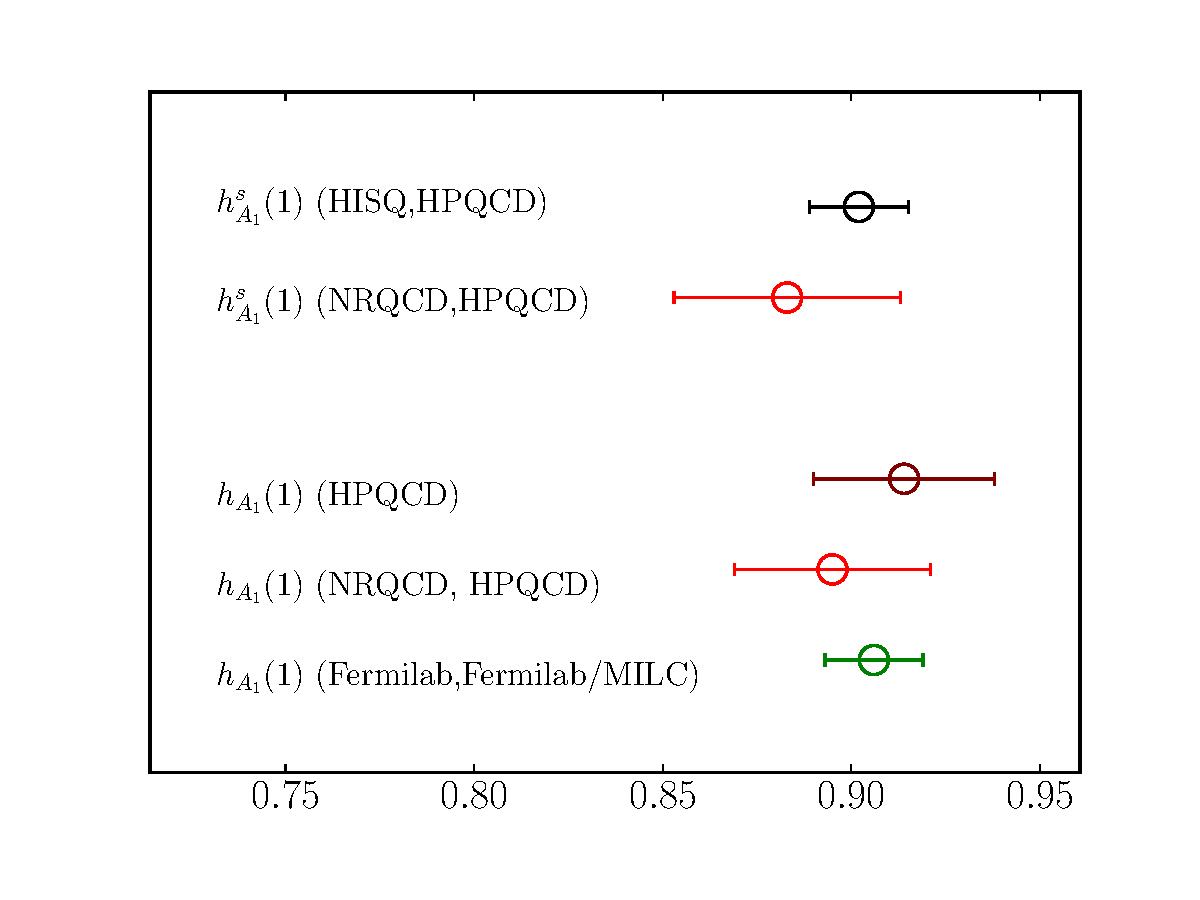
\includegraphics[width=0.7\textwidth]{images/BsDsstar/comparisons.pdf}
  \caption{ $h_{A_1}^{(s)}(1)$ from different calculations. Our result is marked (HISQ,HPQCD). Those marked (NRQCD,HPQCD) are from \cite{Harrison:2017fmw}. The quantity marked (HPQCD) is the result of multiplying our result for $h^s_{A_1}(1)$ with the ratio $h_{A_1}(1)/h^s_{A_1}(1)$ computed at \cite{Harrison:2017fmw}. The quantity marked (Fermilab,Fermilab/MILC) is from \cite{Bailey:2014tva}. \label{fig:comparison_BsDsstar}}
  \end{center}
\end{figure}

\begin{figure}[htb!]
  \vspace{-20pt}
  \begin{center}
  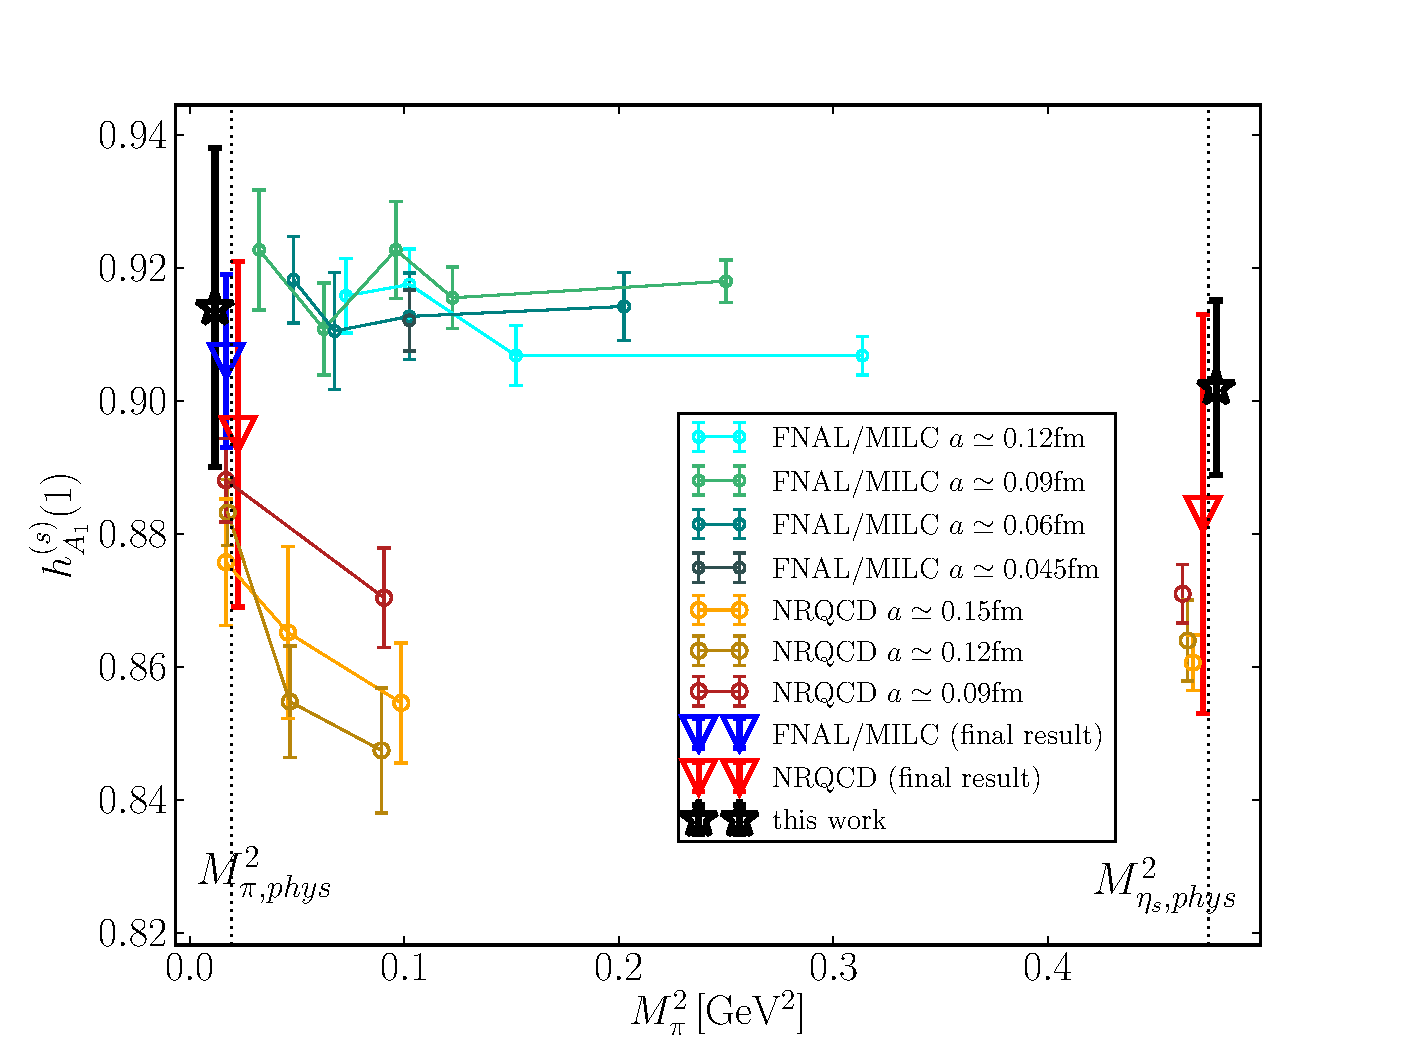
\includegraphics[width=0.9\textwidth]{images/BsDsstar/fermilab_nrqcd_data.pdf}
  \caption{Lattice data and continuum extrapolated data for three studies of $h_{A_1}(1)$ and $h_{A_1}^s$, against the pion mass. Points labeled FNAL/MILC are from \cite{Bailey:2014tva}, and those labeled NRQCD are from \cite{Harrison:2017fmw}. The x-axis must be taken with a pinch of salt, the points at $M_{\pi}=M_{\eta_s}$ have pions in the sea of smaller masses than $M_{\eta_s}$, but we place them here to signify that the spectator quark as the mass of a strange quark. \label{fig:fermilab_data}}
  \end{center}
  \vspace{-20pt}
\end{figure}

\subsection{HQET Low Energy Constants}

%% \begin{table}
%%   \begin{center}
%%     \begin{tabular}{c c c c}
%%       \hline
%%       Source & $l_V$ & $l^s_A$ & $l^s_P$ \\ [0.5ex]
%%       \hline
%%       Statistics & 30.3 & 101.8 & 64.4  \\ [1ex]
%%       $a\to 0$ & 22.4 & 80.5 & 38.2 \\ [1ex]
%%       mistuning & 2.0 & 3.5 & 1.5  \\ [1ex]
%%       $\eta_A$ & 0.7 & 0.7 & 0.7 \\ [1ex]
%%       $\order{1/m_c^3}$ & 4.4 & - & -\\ [1ex]
%%       \hline
%%       Total & 40.0 & 136.9 & 78.9  \\ [1ex]
%%       \hline
%%     \end{tabular}
%%   \end{center}
%%   \caption{Error budget for HQET low energy constants. Each column gives the \% fractional error for the associated quantity. \label{tab:HQETbudget}}
%% \end{table}

Our fit of the lattice data to our fit function (Eq. \eqref{eq:fitform_BsDsstar}) produced the fit parameters $l_{V,A,P}$, which as discussed in Sec. \ref{sec:BsDsstar_heavymass} are numerically approximately equal to the low energy HQET constants of the same name. We find
\begin{align}
  \nonumber  l_V &= 0.71(28)\text{GeV}^2, \\  l_A &= -0.34(32)\text{GeV}^2, \label{eq:hqet_constants_hA1}
  \\ \nonumber l_P &= -0.53(34)\text{GeV}^2.
\end{align}
% These are the first lattice determinations of these quantities. %Not sure if this is true!!
An estimate from the ISGW model for $B\to D^*$ decays gives \cite{PhysRevD.39.799}
\begin{align}
  l_P \simeq l_V \simeq 0.39\text{GeV}^2.
\end{align}
One does not expect these to differ significantly from the $B_s\to D_s^*$ case. These are of the same order of magnitude as our results.

\subsection{Extrapolation Stability}
\label{sec:stability_BsDsstar}

\begin{figure}%[htb!]
  \begin{center}
  \hspace{-18pt}
  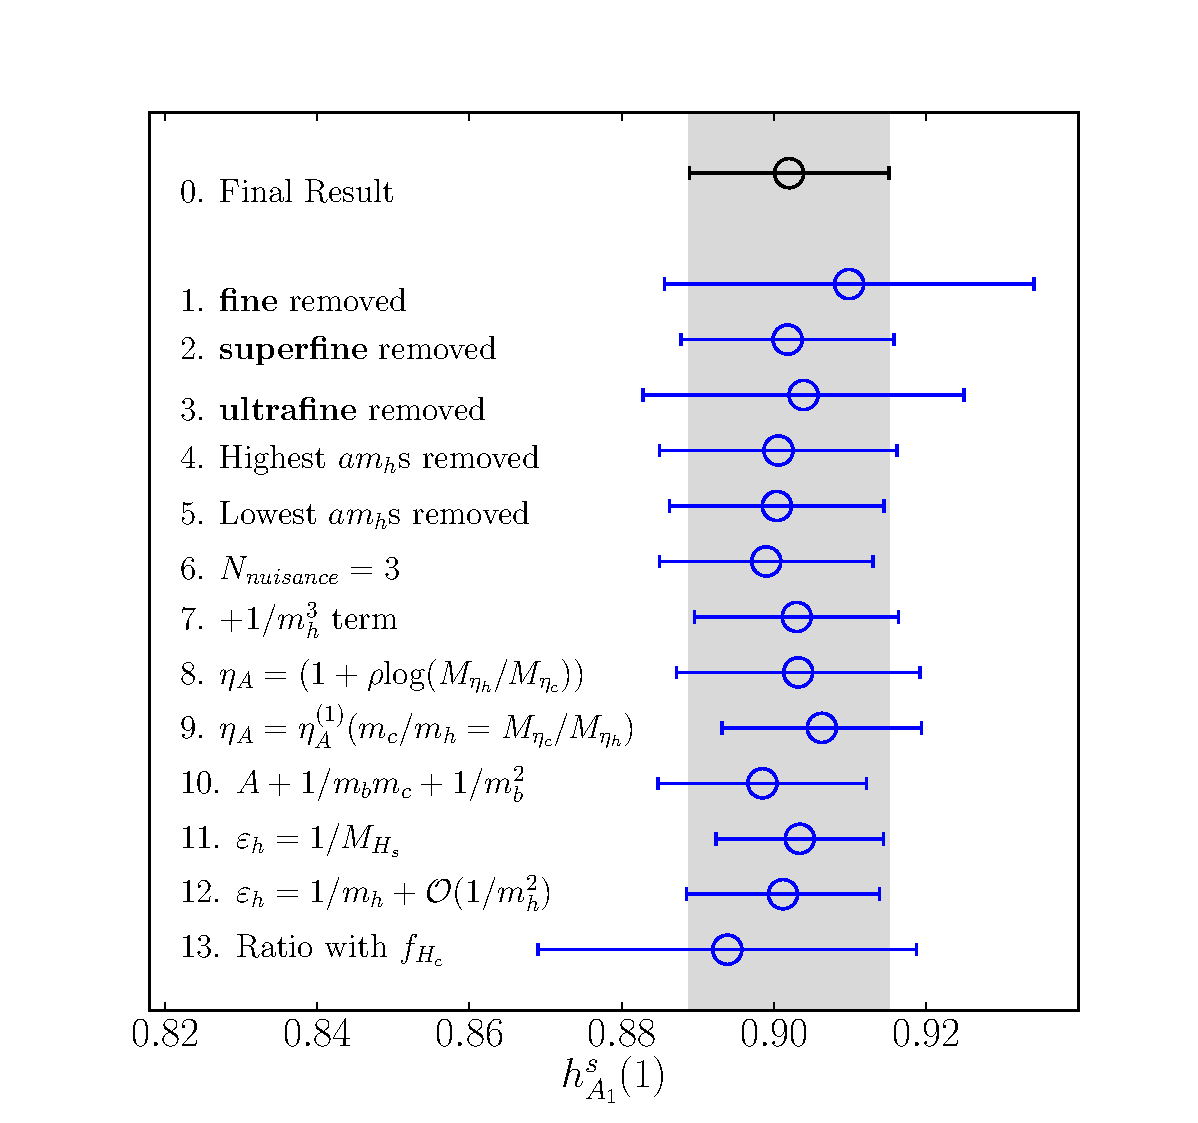
\includegraphics[width=0.8\textwidth]{images/BsDsstar/hA1vsmh_fittests.pdf}
  
  \caption{Results of $h_{A_1}^s(1)$ extrapolation tests. The top three blue points show the final result if data from the fine, superfine or ultrafine ensembles are not used in the fit.
    The fourth and fifth blue points show the result if data at the highest/lowest $am_{h0}^{\text{val}}$ value on each ensemble are removed.
    '$N_{\text{nuisance}}=3$' shows the result of truncating each sum in $\mathcal{N}_{\text{disc}}$ (Eq. \eqref{eq:fitfun_hA1}) at 3 rather than 2.
    '$+1/m_b^3$' results from adding an extra term to \eqref{eq:fitform_BsDsstar} of the form $p/M_{\eta_h}^3$ where $p$ is a fit parameter with the same prior as $l_{V,A,P}^s$. In this case, the Bayes factor falls by a factor of 7, suggesting that the data does not contain a cubic dependence on the heavy mass.
    The next two points show the results of the implementations of $\eta_A$ described in Sec. \ref{sec:BsDsstar_extrapolation}. $\rho$ is a fit parameter with prior distribution $0\pm 1$. Including this factor causes the Bayes factor to drop by a factor of 20, implying that the data cannot resolve logarithms in $m_h$. The second point shows the result of using the 1-loop expression for $\eta_A$ (Eq. \eqref{eq:etaA}), with $m_c/m_h$ replaced with $M_{\eta_c}/M_{\eta_h}$.
    '$A+1/m_bm_c+1/m_b^2$' is the result of replacing $1+l_V/m_c^2$ in the fit with simply a fit parameter $A$ with prior distribution $1\pm 1$. The fact that this does not affect the fit implies that charm mistuning does not strongly affect the extrapolation.
    The two points after that show the result of replacing the heavy mass proxy $M_{\eta_h}/2$ with $M_{H_s}$ and $\varepsilon_h$ (Eq. \eqref{eq:epsilon_h}) respectively.
    The point labelled 'Ratio with $f_{H_c}$' is the result of an alternative extrapolation described in Sec. \ref{sec:stability_BsDsstar}.  \label{fig:fittests_hA1}}
    \end{center}
\end{figure}


We performed a number of tests of the continuum/heavy mass extrapolation. The results of each of these tests are given in Fig. \ref{fig:fittests_hA1}.

One of the tests requires some explaination, the result of which is given in Fig. \ref{fig:fittests_hA1}, labelled 'Ratio with $f_{H_c}$'. We performed a continuum/heavy mass extrapolation in the ratio $h_{A_1}^s(1)/(f_{H_c}\sqrt{M_{H_c}})$. $f_{H_c}$ is found from fitting the $H_c$ correlation functions to obtain $a_0^{H_c}$, and using Eq. \eqref{eq:decayconstant_pseudoscalar}. Since we create the $H_c$ mesons with a local HISQ pseudoscalar current, which is absolutely normalized, no renormalization of $f_{H_c}$ is required here. Details of the extrapolation are given below.

Discretization effects cancel to a large extent in this ratio. It however varies strongly with changing heavy mass. This makes the extrapolation very different from the extrapolation in $h_{A_1}^s(1)$, which has large discretization effects but has little variation in the heavy mass. The two extrapolations have quite different systematics, so testing their agreement is a stringent test of our formalism.

In order to compare the result of the two extrapolations, we must multiply $h_{A_1}^s(1)/(f_{B_c}\sqrt{M_{B_c}})$ by $f_{B_c}\sqrt{M_{B_c}}$. We can use the PDG value for $M_{B_c}$ \cite{PhysRevD.98.030001}. For an $f_{B_c}$ value, we extrapolate our $f_{H_c}$ data to the physical point.

We used a similarly structured fit form for both the $h_{A_1}^s(1)/(f_{B_c}\sqrt{M_{B_c}})$ and $f_{H_c}$ extrapolations. We followed the methodology of \cite{McNeile:2012qf}. Both extrapolations use a fit function of the form
\begin{align}
  \label{eq:fitfun_ratio}
  \nonumber
  \text{fit} = &A\left({\alpha_s(M_{\eta_h}/2)\over\alpha_s(M_{\eta_c}/2)}\right)^{6s/25} M_{\eta_h}^{n/2} \sum_{i,j,k=0}^{2,2,2} d_{ijk} \left({2\text{GeV}\over M_{\eta_h} }\right)^{i} \left({ am^{\text{val}}_{h0} \over \pi }\right)^{2j} \left({ am^{\text{val}}_{c0} \over \pi }\right)^{2k} \\
  &\quad \times\left( 1 + \mathcal{N}_{\text{mistuning}} + \mathcal{N}^c_{\text{mistuning}} \right)\,.
\end{align}
$\alpha_s(M)$ is the QCD coupling evaluated at scale $M$ (according to results from \cite{Chakraborty:2014aca} with $N_f=5$). $s=+1$ and $n=0$ for $h_{A_1}^s(1)/(f_{H_c}\sqrt{M_{H_c}})$, $s=-1$ and $n=-1$ for $f_{H_c}$. The $M_{\eta_h}^{n/2}$ accounts for the leading order dependence of $f_{H_c}$ in HQET, and the $\alpha_s$ ratio comes from renormalization group improved matching between QCD and HQET of $f_{H_c}$. $\mathcal{N}_{\text{mistuning}}$ is defined in Eq. \eqref{eq:mistuning_BsDsstar}. We have introduced a new mistuning term for the charm:
\begin{align}
  \mathcal{N}^c_{\text{mistuning}} = c_c \left({M_{\eta_c}-M_{\eta_c}^{\text{phys}}\over M_{\eta_c}^{\text{phys}}}\right)\,,
  \label{eq:charmmistuning_BsDsstar}
\end{align}
where $M_{\eta_c}^{\text{phys}}$ is taken from the PDG \cite{PhysRevD.98.030001}, and $c_c$ is a fit parameter with prior distribution $0\pm 1$.

$A$ is given prior distribution $0\pm 4$GeV$^{3/2}$ in the $f_{H_c}$ case and $0\pm 2$GeV$^{-3/2}$ in the ratio case. $d_{ijk}$ are given priors of $0\pm 2$ in all cases except $d_{000}$ which is set to 1.

\begin{figure}[htb!]
  \begin{center}
  \hspace{-10pt}
  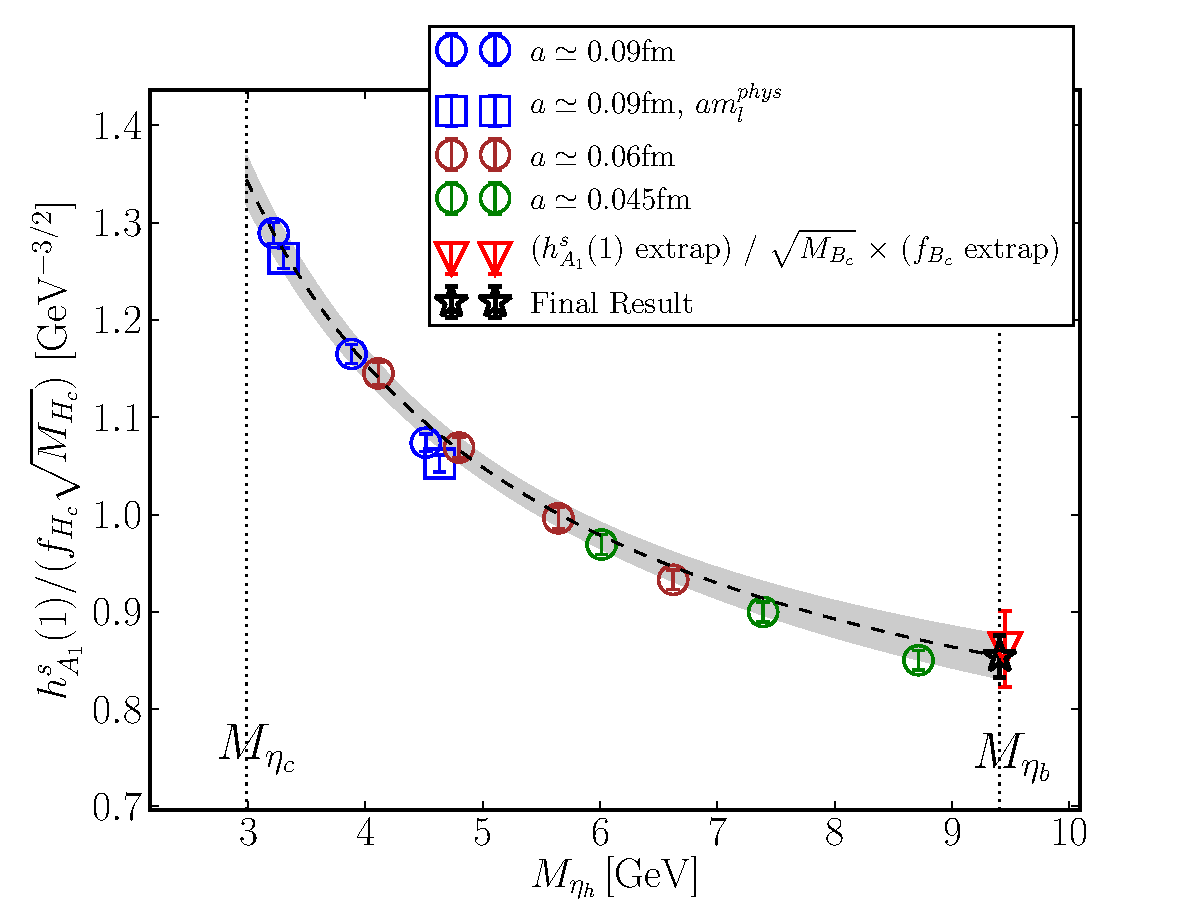
\includegraphics[width=0.70\textwidth]{images/BsDsstar/hA1overfHc.pdf}
  \caption{ $h_{A_1}^s(1)/(f_{H_c}\sqrt{M_{H_c}})$ against $M_{\eta_h}$ (a proxy for the heavy quark mass). The grey band shows the result of the extrapolation at $a=0$ and physical $l$,$s$ and $c$ masses. Sets listed in the legend follow the order of sets in Table \ref{tab:BsDsensembles}. The black point shows our final result for $h_{A_1}^s(1)$ divided by $\sqrt{M_{B_c}}$ from the PDG \cite{PhysRevD.98.030001} and $f_{B_c}$ from our extrapolation of $f_{H_c}$ to continuum and physical $b$ mass.
    \label{fig:fHc}}
  \end{center}
\end{figure}


The result of the extrapolation of $h_{A_1}^s(1)/(f_{H_c}\sqrt{M_{H_c}})$ at the physical point was multiplied by our $f_{B_c}M_{B_c}$ result to obtain a second determination of $h_{A_1}^s(1)$. This is the result given in Fig. \ref{fig:fittests_hA1} labelled 'Ratio with $f_{H_c}$'.

The extrapolation in $f_{H_c}$ is shown in Fig. \ref{fig:fHc_vsmh}. We here include the result from a previous heavy-HISQ determination of $f_{B_c}$ on $N_f=2+1$ MILC ensembles \cite{McNeile:2012qf}. Our final result for this quantity is
\begin{align}
  f_{B_c} = 0.4178(45)\,\text{GeV}\,.
\end{align}

\begin{figure}[htb!]
  \begin{center}
  \hspace{-20pt}
  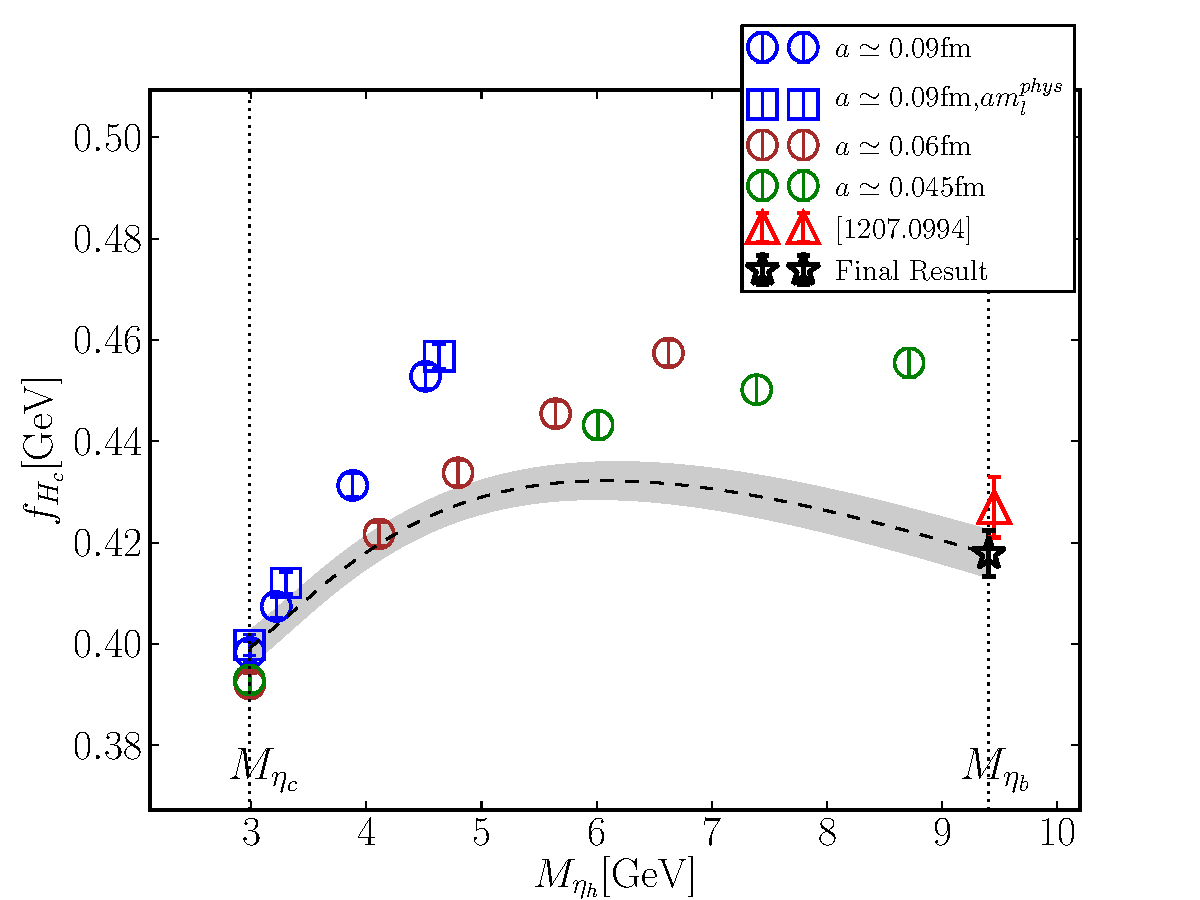
\includegraphics[width=0.80\textwidth]{images/BsDsstar/fHcvsmh.pdf}
  \caption{ $h_{A_1}^s(1)$ against $M_{\eta_h}$ (a proxy for the heavy quark mass). The grey band shows the result of the extrapolation at $a=0$ and physical $l$,$s$ and $c$ masses. Sets listed in the legend follow the order of sets in table \ref{tab:BsDsensembles}. The red point shows the result from a previous heavy-HISQ determination of $f_{B_c}$ on 2+1 gauge ensembles \cite{McNeile:2012qf}. \label{fig:fHc_vsmh}}
  \end{center}
\end{figure}

\subsection{$H_s$ and $D_s^*$ Masses}

As a further consistency check of our results, we can check if the masses for the $H_s$ and $D_s^*$ mesons, extracted from our correlator fits, reproduce what we expect physically.

Fig. \ref{fig:Dsmasses} shows $D_s^*$ mass extracted from correlators on each ensemble. Each are consistent with the experimentally measured $D_s^*$ mass (the grey band).

We performed an extrapolation of $M_{H_s}-M_{\eta_h}/2$ masses to continuum $m_h=m_b$ {\textit{and}} $m_h=m_c$, for comparison with the known value for $M_{B_s}-M_{\eta_b}/2$ and $M_{D_s}-M_{\eta_c}/2$. To perform this extrapolation we use the fit form
\begin{align}
  %% \left(M_{H_s}-{M_{\eta_h}\over2}\right)\Big|_{\text{fit}} =& \left({M_{\eta_h}\over 2\text{GeV}}\right) \sum_{i,j=0}^{2,2,2} d_{ijk} \left({2\text{GeV}\over M_{\eta_h} }\right)^{i} \left({ am^{\text{val}}_{h0} \over \pi }\right)^{2j} \left({ a\Lambda_{\text{QCD}} \over \pi }\right)^{2k} \\
  %% &+ \mathcal{N}_{\text{mistuning}} + \mathcal{N}^c_{\text{mistuning}}\,,
  %% \nonumber
  \left(M_{H_s}-{M_{\eta_h}\over2}\right)\Big|_{\text{fit}}& =
  \left( \sum_{n=-1}^{+1} c_n \left({M_{\eta_h}\over 2\text{GeV}}\right)^n\right) \times
  \\ &\left( 1 + \sum_{i,j=0}^{2,2} d_{ij} \left({ am_{h0}^{\text{val}} \over \pi }\right)^{2i} \left({ a\Lambda_{\text{QCD}} \over \pi }\right)^{2j} + \mathcal{N}_{\text{mistuning}} \right)\,.
    \nonumber
\end{align}
$c_n$ are fit parameters. Since the lattice data for $M_{H_s}-M_{\eta_h}/2$ is close to linear, priors can be set for $c_{1}$ and $c_0$ by inspecting the approximate gradient and intercept of $\left(M_{H_s}-{M_{\eta_h}/2}\right)$ against $M_{\eta_h}$. Accordingly $c_{1}$ is given prior 0.05(5), and $c_0$ is given 0.5(5). $c_{-1}$ is given $0\pm 1$. $d_{ij}$ are given priors $0\pm 1$.  $\mathcal{N}_{\text{mistuning}}$ is defined in Equation \eqref{eq:mistuning_BsDsstar}. We tested the effect of including $\order{1/M_{\eta_h}^2}$ and $\order{1/M_{\eta_h}^3}$ terms, this does not change the result in any statistically significant way.

Fig. \ref{fig:MHsmasses} depicts this extrapolation. We find
\begin{align}
  &M_{B_s} - {M_{\eta_b}\over 2} =  0.6588(61) \text{GeV}\,, \\
  &M_{D_s} - {M_{\eta_c}\over 2} =  0.4755(37)  \text{GeV}\,.
\end{align}
As can be seen from Fig. \ref{fig:MHsmasses}, both are in agreement with the physical result.

\begin{figure}[htb!]
  \begin{center}
  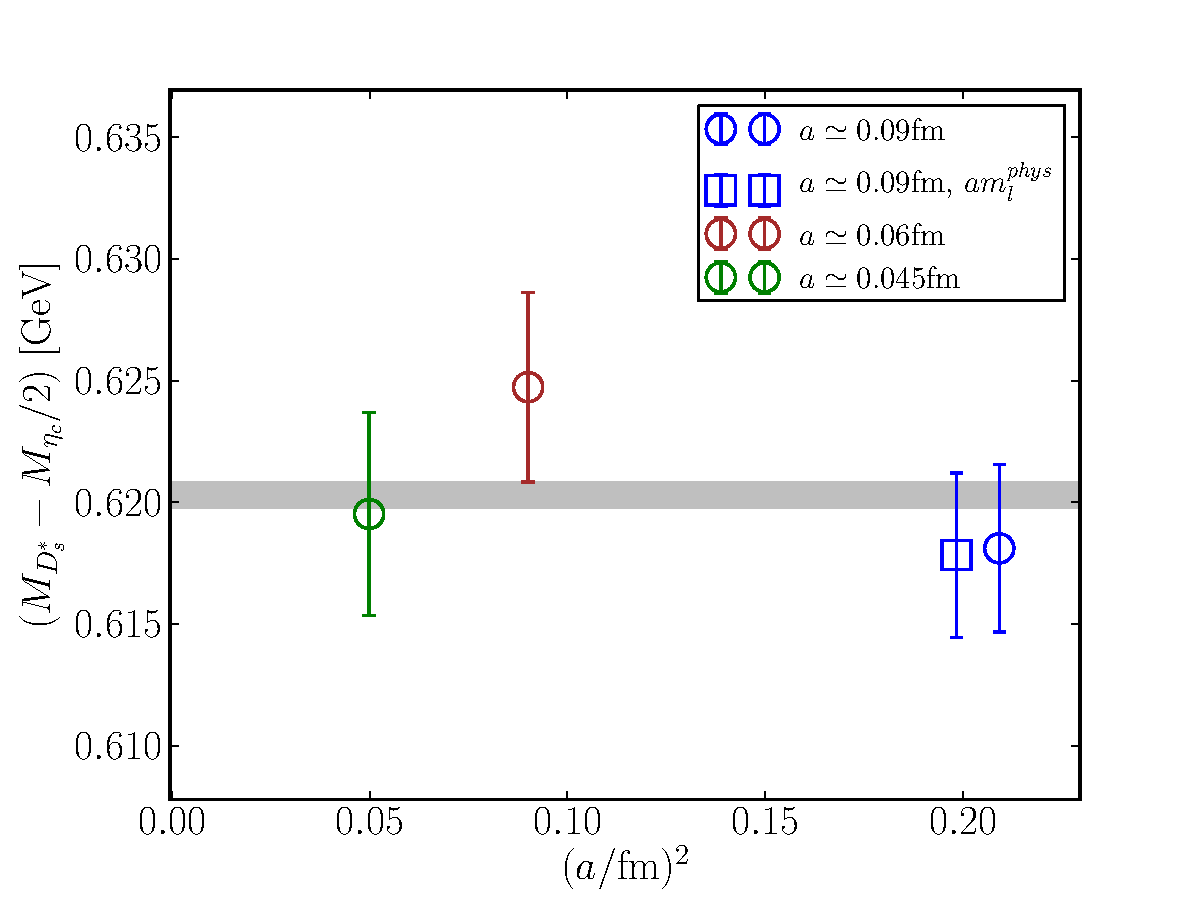
\includegraphics[width=0.70\textwidth]{images/BsDsstar/Dsmasses.pdf}
  \caption{Lattice results for $M_{D_s^*}-M_{\eta_c}/2$ on each ensemble.The grey band shows the PDG result \cite{PhysRevD.98.030001}. \label{fig:Dsmasses}}
  \end{center}
\end{figure}

\begin{figure}[htb!]
  \begin{center}
  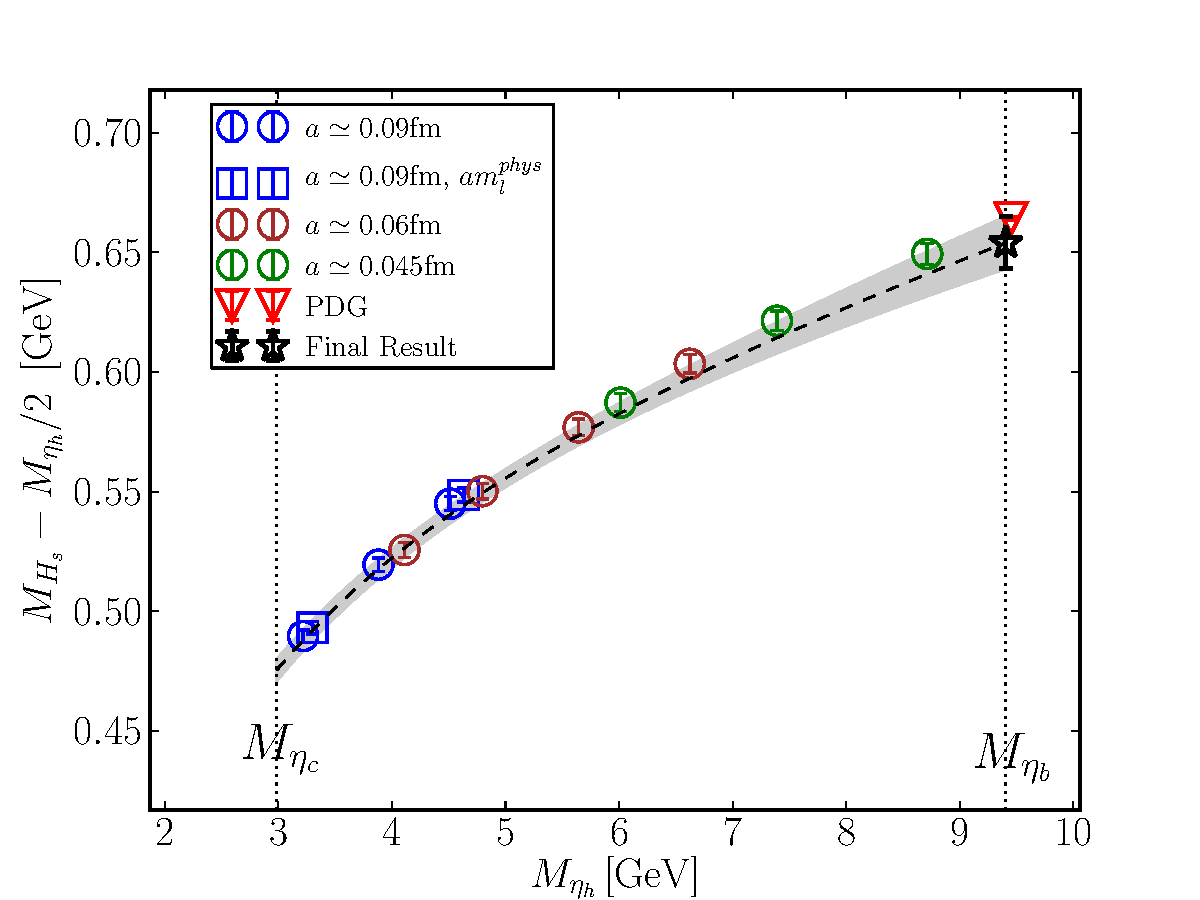
\includegraphics[width=0.80\textwidth]{images/BsDsstar/MHs-Metah.pdf}
  \caption{Extrapolation of $M_{H_s}-M_{\eta_h}/2$ to the physical point.The grey band shows the result at $a=0$ and physical charm, strange and light masses. \label{fig:MHsmasses}}
  \end{center}
\end{figure}

\section{Conclusions}
\label{sec:conclusions}

We have produced a fully non-perturbative determination of $h_{A_1}^s(1)$, sometimes called $\mathcal{F}^{B_s\to D_s}(1)$, using unquenched lattice data from a fully relativistic and highly improved lattice action, along with an estimation of the low energy constants $l_{V,A,P}$, given in \eqref{eq:finalresult_hA1} and \eqref{eq:hqet_constants_hA1} respectively. We used gauge ensembles with 3 lattice spacings, including an ensemble with approximately physical light sea quark masses, and obtained data corresponding to 12 different heavy quark masses.

This study supplies an independent check of the NRQCD formalism used in previous HPQCD studies. It is also much more precise, in the case of $h_{A_1}^s$, the total fractional error has been halved in comparison to the NRQCD determination. The comparative precision resulting from the heavy-HISQ method suggests that it is well suited to computing other form factors associated with $b$-decays.

This study also clearly demonstrates the power of the heavy-HISQ approach. It produces a result approximately twice as precise as the NRQCD result and contains fewer assumptions while being consistent with all other lattice studies of $h^s_{A_1}(1)$ and $h_{A_1}(1)$. 

%% Various improvements to this study could be implemented in future calculations. For example - since the uncertainty is dominated by statistics, more lattice data should be included. One useful innovation that was not used here is the Covariant Approximation Averaging approach to solving quark propagators \cite{PhysRevD.91.114511}, this could significantly boost statistics while keeping the computational cost manageable.
%% %%

 % Bs-Ds* at zero recoil with Heavy HISQ
\chapter{$B_s\to D_sl\nu$ Form Factors at All Physical $q^2$ from Heavy-HISQ}
\label{chap:BsDs}

In this chapter, I present the second of our two heavy-HISQ studies, the calculation of the $B_s\to D_sl\nu$ form factors $f^s_0(q^2)$ and $f^s_+(q^2)$ throughout all physical $q^2$, as defined in Sec. \ref{sec:weakdecays}. Like for $h_{A_1}^s(1)$, I'm giving this quantity the superscript $s$ to differentiate it from the more often referred to form factors for $B\to Dl\nu$ decays.

I here briefly review the definition of the form factors here for ease of reading. The differential decay rate for $B_s\to D_s l \nu$ decays are given in the SM by \cite{PhysRevD.98.030001}:
\begin{align}
  &{d\Gamma\over dq^2} = \eta_{\text{EW}} { G_F^2 |V_{cb}|^2\over 24 \pi^3 M_{B_s}^2 } \left( 1 - {m_l^2\over q^2}\right)^2 |{\bf{p}}_{D_s}| \,\,\times \\
  \label{eq:branchingfraction}
  &\left[ \left( 1 + {m_l^2\over 2q^2}\right) M_{B_s}^2 |{\bf{p}}_{D_s}|^2 f_+^{s\,2}(q^2) + {3m_l^2\over 8q^2} (M_{B_s}^2-M_{D_s}^2)^2 f_0^{s\,2}(q^2) \right] \nonumber
\end{align}
where $m_l$ is the mass of the lepton, $\eta_{\text{EW}}$ is the electroweak correction \cite{SIRLIN198283,Ginsberg1968,PhysRevD.41.1736}, $q^2 = (p_{B_s} - p_{D_s})^2$ is the momentum transfer, and $f_0^s(q^2)$, $f_+^s(q^2)$ are the scalar and vector form factors that parameterize the non-perturbative contribution to the decay. The allowed range of $q^2$ values if the final states are on-shell is
\begin{align}
  m_l^2 \leq q^2 \leq (M_{B_s}-M_{D_s})^2.
\end{align}
The form factors parameterize matrix elements of the electroweak current between $B_s$ and $D_s$ states, $\langle D_s | (V-A)_{\mu} | B_s \rangle$ where $V_{\mu}=\bar{b}\gamma_{\mu}c$ is the vector component and $A_{\mu}=\bar{b}\gamma_5\gamma_{\mu} c$ is the axial vector component. In a pseudoscalar-to-pseudoscalar amplitude, only $V_{\mu}$ contributes, since $\langle D_s | A_{\mu} | B_s \rangle$ does not satisfy the parity invariance of QCD. The vector current in terms of form factors is given by
\begin{align}
  \langle D_s | V^{\mu} | B_s \rangle &= f_+^s(q^2) \left[ p_{B_s}^{\mu} + p_{D_s}^{\mu} - {M_{B_s}^2 - M_{D_s}^2 \over q^2} q^{\mu} \right] \nonumber \\
  &+ f_0^s(q^2) { M_{B_s}^2 - M_{D_s}^2 \over q^2} q^{\mu}\,.
  \label{eq:vectorcurrent}
\end{align}
Analyticity of this matrix element demands that
\begin{align}
  f_+^s(0) = f_0^s(0)\,.
  \label{eq:q20constraint}
\end{align}
Via the PCVC relation, the form factor $f_0^s(q^2)$ is also directly related to the matrix element of the scalar current $S=\bar{b}c\,$:
\begin{align}
  (m_b-m_c)\langle D_s | S | B_s \rangle = (M^2_{B_s} - M^2_{D_s}) f_0^s(q^2)\,.
    \label{eq:scalarcurrent}
\end{align}
In our calculation we access the form factors by computing matrix elements of the temporal vector current $V_0$ and the scalar current $S$. The form factors can be extracted from this combination using expresions derived from equations \eqref{eq:vectorcurrent} and \eqref{eq:scalarcurrent}:
\begin{align}
  f_0^s(q^2) &= {m_b - m_c\over M_{B_s}^2 - M_{D_s}^2 } \langle D_s | S | B_s \rangle, \\
  f_+^s(q^2) &= {1\over 2M_{B_s}} { \delta^M \langle D_s | S | B_s \rangle - q^2 \langle D_s | V_0 | B_s \rangle \over {\bf{p}}^2_{D_s}}, \\
    &( \, \delta^M = (m_b - m_c)(M_{B_s}-E_{D_s}) \, ). \nonumber
\end{align}

Our goal is to compute $f_0^s(q^2)$ and $f_+^s(q^2)$ throughout the range of $q^2$ values $0 \leq q^2 \leq (M_{B_s}-M_{D_s})^2 \equiv q^2_{\text{max}}$. We extend the range to $q^2=0$ in order to take advantage of the constraint in Eq. \eqref{eq:q20constraint}. To achieve this, we compute $\langle D_s | S | H_s \rangle$ and $\langle D_s | V_0 | H_s \rangle$ on the lattice, where the $H_s$ meson is at rest and $D_s$ mesons are given an appropriate array of spatial momenta.

%Those interested in simply using the form factors calculated here should refer to Sec. \ref{sec:reconstructing_formfactors}, which gives all information necessary for reconstructing our form factors.

\section{Motivation}
\label{sec:BsDs_intro}

%% The decays of heavy measons like the $B$ and $B_s$ is a potential source of insights into physics beyond the Standard Model (SM). Namely, quark flavour-changing $B$ decays have gained much interest due to a number of related tensions between experimental measurements and SM predictions \cite{Wei:2009zv,Lees:2012xj,Lees:2012tva,Lees:2013uzd,Aaij:2014pli,Aaij:2014ora,Huschle:2015rga,Aaij:2015oid,Aaij:2015yra,Aaij:2015xza,Aaij:2016flj,Wehle:2016yoi,Sato:2016svk,Hirose:2017dxl,Aaij:2017deq,Aaij:2017uff,Aaij:2017vbb,Sirunyan:2017dhj,Aaboud:2018krd}.
%Discrepancies between systematically independent determinations of Cabibbo-Kobayashi-Maskawa (CKM) matrix elements \cite{Amhis:2016xyh,Bevan:2014iga,Alberti:2014yda} have also sparked interest. 

$B_s\to D_s l\nu$ decays can supply a new method for precisely determining the CKM element $|V_{cb}|$. Determination of $|V_{cb}|$ in this way requires both a measurement of the branching fraction and a theoretical determination of the form factors, as explained in Sec. \ref{sec:weakdecays}. To obtain the highest possible precision, data for both the form factors and branching fractions are required throughout the largest possible range of momentum transfer. Analogous approaches were already performed using $B\to D l \nu$ decays \cite{Buskulic:1996yq,Bartelt:1998dq,Aubert:2008yv,Aubert:2009ac,Lattice:2015rga,Na:2015kha,Glattauer:2015teq}. 

The $B_s\to D_s l\nu$ decay can also supply a new test of the SM, by comparing the theoretical and experimental determinations of the ratio $R_{D_s}$, defined in Eq. \eqref{eq:Rratios}. This would be especially illuminating since tension has been found in the intimately related ratios $R_{D^{(*)}}$. The presence or absence of an anomaly in $R_{D_s}$ would help to confirm or dismiss a new physics explanation for such a family of anomalies.

The $B_s\to D_s l\nu$ scalar form factor is useful in the experimental extraction of $B_s \to \mu^+\mu^-$ branching fractions. Taking a ratio of the $B_s\to D_s$ and $B\to D$ scalar form factors gives the so-called fragmentation ratio, the ratio of probabilities of a $b$ quark hadronizing into a $B$ or $B_s$ meson. In analyses such as \cite{CMS:2014xfa}, $B_s \to \mu^+\mu^-$ branching fractions are measured using $B_u^+\to J/\psi(\mu^+\mu^-)K^+$ and $B_d^0\to K^+\pi_-$ as normalization channels, in this case one requires a value for the fragmentation ratio.

Similar to the $B_{(s)}\to D_{(s)}^*$ case, chiral perturbation theory implies that form factors for $B_s \to D_s$ and $B \to D$ decays are insensitive to the mass of the spectator quark, implying that form factors for these two decays are approximately equal \cite{Laiho:2005ue}. This expectation has been validated by previous lattice calculations, for example in \cite{PhysRevD.85.114502} the ratio of scalar form factors for the two decays at momentum transfer $q^2=M^2_{\pi}$ was found to be $f^s_0(M_{\pi}^2)/f_0(M_{\pi}^2) = 1.054(50)$, while \cite{Monahan:2017uby} found the value $f^s_0(M_{\pi}^2)/f_0(M_{\pi}^2) = 1.006(62)$. Hence we can expect to learn about $B\to D$ form factors by studying $B_s\to D_s$. 

While $B\to D$ form factors are currently more phenomenologically useful, $B_s\to D_s$ form factors are more attractive on the lattice QCD side. The absence of valence light ($u$ or $d$) quarks means lattice QCD results have smaller statistical errors, are less computationally expensive, have a more simple chiral extrapolation to the physical light mass, and negligible finite volume effects. This makes the $B_s \to D_s l\nu$ decay a useful test bed for lattice techniques that may be later used to study $B \to D l \nu$ decays.

A number of lattice calculations of $B_{(s)} \to D_{(s)}$ form factors have already been performed. The FNAL/MILC collaboration produced $B\to D$ form factors on the $N_f=2+1$ MILC gluon ensembles using the Fermilab action for $b$ and $c$ valence quarks and ASQTAD light quarks \cite{Lattice:2015rga}. They also, in an earler work, computed the ratio of scalar form factors for $B_s\to D_s$ and $B\to D$ to obtain the fragmentation ratio \cite{PhysRevD.85.114502}. The HPQCD collaboration computed both $B\to D$ and $B_s\to D_s$ form factors on the $N_f=2+1$ MILC gluon ensembles using the NRQCD action for the valence $b$, and the HISQ action for all other quarks \cite{Na:2015kha,Monahan:2017uby}. Atoui et. al. also produced $B_s\to D_s$ form factors using maximally twisted Wilson quarks on $N_f=2$ gluon ensembles \cite{Atoui2014}. A calculaton of the $B_s\to D_s$ form factors by the RBC/UKQCD collaboration is currently underway \cite{RBCmichigan}.

A considerable limitation in the FNAL/MILC and HPQCD studies is the requirement for perturbative matching between the lattice effective field theories and continuum QCD. FNAL/MILC required a matching that was only available to 1-loop, resulting in an $\mathcal{O}(\alpha_s^2)$ systematic error. In the HPQCD calculation, NRQCD-HISQ currents were truncated, prompting them to report large systematic errors. Besides the reported errors, as was discussed in Chapter \ref{chap:nrqcd}, parts of the NRQCD-HISQ vector current that contribute away from zero recoil have a large magnitude ($\sim 30\%$ of the leading order). The currents used in this study did not take these large subleading currents into account, so the result from this may have large uncontrolled systematic errors.

Another limitation present in each of the aforementioned studies is that the lattice data is limited to a region of high $q^2$. To generate lattice points at lower $q^2$, a large spatial momentum must be given to one of the quarks on the lattice. Due to signal/noise degradation, adding momentum leads to an exponential increase of noise in correlation functions. Hence, in cases like $B_{(s)}\to D_{(s)}$, lattice data close to $q^2=0$ would be uselessly noisy. Lattice results must be limited to high $q^2$. This fact necessitates an extrapolation from the data in the high $q^2$ region to the rest of the physical range. Since there has been some controversy in choices of form factor extrapolations through $q^2$ recently (for example see \cite{Bigi:2017njr,Grinstein:2017nlq}), it would be desirable to instead have lattice data covering the entire $q^2$ range. We can in fact achieve this with the heavy-HISQ approach. This is because in heavy-HISQ the $b$ quarks are lighter than physical, this shrinks the $q^2$ range, meaning smaller spatial momenta are required to cover the range.


\section{Calculation Details}
\label{sec:lattice}

\subsection{Lattice Setup}

%% \begin{table*}[htb!]
%%   \begin{center}
%%     \begin{tabular}{c c c c c c c c c c}
%%       \hline
%%       set & handle & $a/$fm  & $N_x^3\times N_t$ & $am_{l0}$ & $am_{s0}$ & $am_{c0}$  \\ [0.5ex]
%%       \hline
%%       1 & \bf{fine} & 0.0884(6) & $32^3\times96$ & 0.0074 & 0.037 & 0.440 \\ [1ex]
%%       2 & \bf{fine-physical} & 0.0873(5) & $64^3\times96$ & 0.0012 & 0.0363 & 0.432 \\ [1ex]
%%       3 & \bf{superfine} & 0.05922(12) & $48^3\times144$ & 0.0048 & 0.024 & 0.286 \\ [1ex]
%%       4 & \bf{ultrafine} & 0.04406(23) &  $64^3\times192$ & 0.00316 & 0.0158 & 0.188  \\ [1ex]
%%       \hline
%%     \end{tabular}
%%   \end{center}
%%     \caption{Parameters for gluon ensembles \cite{Bazavov:2010ru,Bazavov:2012xda}. $a$ is the lattice spacing, values for sets 1 \& 2 deduced in \cite{Dowdall:2013rya}, set 3 from \cite{Chakraborty:2014aca}. We thank C. McNeile for computing the $a$ value on set 4. These $a$ values are determined by measuring the Wilson flow parameter $w_0/a$ on the lattice, then using the known value for $w_0$ to isolate $a$. $N_x$ is the spatial extent and $N_t$ the temporal extent of the lattice. Light, strange and charm quarks are included in the sea, their masses are given in columns 5-7. \label{tab:ensembles}}
%% \end{table*}

%% \begin{table*}[htb!]
%%   \begin{center}
%%     \begin{tabular}{c c c c c c c c c c}
%%       \hline
%%       set & $am_{s0}^{\text{val}}$ & $am_{c0}^{\text{val}}$ & $am^{\text{val}}_{h0}$ & $|a{\bf{p}}_{D_s}|$ & $\theta$ & $T$ \\ [0.5ex]
%%       \hline
%%       1 & 0.0376 & 0.45
%%       & 0.5 & 0, 0.056 & 0, 0.328 & 14, 17, 20 \\ [1ex]
%%       & & & 0.65 & 0, 0.142, 0.201 & 0, 0.833, 1.181 & \\ [1ex]
%%       & & & 0.8 & 0, 0.227, 0.323 & 0, 1.334, 1.900 & \\ [1ex]

%%       \hline
%%       2 & 0.036 & 0.433
%%       & 0.5 & 0, 0.0279 & 0, 0.328 & 14, 17, 20 \\ [1ex]
%%       & & & 0.8 & 0, 0.162 & 0, 1.900 & \\ [1ex]

%%       \hline
%%       3 & 0.0234 & 
%%       0.274 & 0.427 & 0, 0.113, 0.161 &  0, 0.998, 1.417  & 22, 25, 28 \\ [1ex]
%%       & & & 0.525 & 0, 0.161, 0.244 & 0, 1.417, 2.151  & \\ [1ex]
%%       & & & 0.65 & 0, 0.244, 0.338 & 0, 2.151, 2.978  & \\ [1ex]
%%       & & & 0.8 & 0, 0.338, 0.438 & 0, 2.978, 3.862  & \\ [1ex]

%%       \hline
%%       4 & 0.0165 
%%       & 0.194 & 0.5 & 0, 0.202, 0.281 & 0, 2.38, 3.306 & 31, 36, 41 \\ [1ex]
%%       & & & 0.65 & 0, 0.202, 0.281, 0.382 & 0, 2.38, 3.306, 4.494  & \\ [1ex]
%%       & & & 0.8 & 0, 0.281, 0.382, 0.473 & 0, 3.306, 4.494, 5.562  & \\ [1ex]
%%       \hline
%%     \end{tabular}
%%   \end{center}
%%   \caption{}
%%   \label{tab:ensembles}
%% \end{table*}

\begin{table*}[htb!]
  \begin{center}
    \begin{tabular}{c c c c c c c c c c}
      \hline
      set & $am_{s0}^{\text{val}}$ & $am_{c0}^{\text{val}}$ & $am^{\text{val}}_{h0}$ & $|a{\bf{p}}_{D_s}|$ & $T/a$ \\ [0.5ex]
      \hline
      1 & 0.0376 & 0.45
      & 0.5 & 0, 0.056 & 14, 17, 20 \\ [1ex]
      & & & 0.65 & 0, 0.142, 0.201 &  \\ [1ex]
      & & & 0.8 & 0, 0.227, 0.323 &  \\ [1ex]

      \hline
      2 & 0.036 & 0.433
      & 0.5 & 0, 0.0279 & 14, 17, 20 \\ [1ex]
      & & & 0.8 & 0, 0.162  & \\ [1ex]

      \hline
      3 & 0.0234 & 
      0.274 & 0.427 & 0, 0.113, 0.161 & 22, 25, 28 \\ [1ex]
      & & & 0.525 & 0, 0.161, 0.244 & \\ [1ex]
      & & & 0.65 & 0, 0.244, 0.338 & \\ [1ex]
      & & & 0.8 & 0, 0.338, 0.438 & \\ [1ex]

      \hline
      4 & 0.0165 
      & 0.194 & 0.5 & 0, 0.202, 0.281 & 31, 36, 41 \\ [1ex]
      & & & 0.65 & 0, 0.202, 0.281, 0.382 & \\ [1ex]
      & & & 0.8 & 0, 0.281, 0.382, 0.473 & \\ [1ex]
      \hline
    \end{tabular}
  \end{center}
  \caption{Simulation details. Columns 2 and 3 give the $s$ and $c$ valence quark masses, which were tuned in \cite{Chakraborty:2014aca}. Column 4 gives the bare heavy quark masses, we use a number of heavy quark masses to assist the extrapolation to the physical $b$ mass. Column 5 gives the absolute value of the spatial momentum given to the $D_s$ meson, using a momentum twist, in lattice units. These values were chosen with the following rationale: when only 2 are used, these correspond to the $q^2=0$ and $q^2_{\text{max}}\,$ points (except on the fine-physical ensemble, where we compute at the points $q^2_{\text{max}}$ and $q^2_{\text{max}}/2$). When 3 twists are used, the momenta correspond to $q^2=0$, $q^2=q^2_{\text{max}}/2$, and $q^2_{\text{max}}$ points. When 4 are used, these are points for $q^2_{\text{max}}$, $3q^2_{\text{max}}/4$, $q^2_{\text{max}}/2$, $q^2_{\text{max}}/4$, $q^2=0$. To give the $D_s$ meson these spatial momenta we gave the charm an appropriate momentum twist in the $(1,1,1)$ direction. Column 6 gives the temporal separations between source and sink, $T$, of the 3-point correlation functions computed on each ensemble.}
  \label{tab:simulation}
\end{table*}

This calculation closely followed the approach employed in our calculation of the $B_s\to D_s^*$ axial form factor at zero recoil, given in the last chapter. The main modifications required for this calculation were 1) the form factors are not protected by Luke's theorem, so a more general fit form for the extrapolation in $m_h$ was required, and 2) to cover the $q^2$ range we gave the charm quark a number of spatial momentum values via a momentum twist (Sec. \ref{sec:momentum_twist}) and interpolate the results to all $q^2$.

We used the same set of ensembles as in the $B_s\to D_s^*$ study. In three of the four ensembles (sets 2, 4 and 5), the bare light mass is set to $m_{l0}/m_{s0} = 0.2$. The fact that the $m_{l0}$ value is unphysically high is expected to have a small effect on the form factors, due to the lack of valence light quarks, and previous experience of the form factor dependence on $m_{l0}$ \cite{Monahan:2017uby}. The small effect due to the unphysical $m_{l0}$ is quantified by including a fourth ensemble (set 3) with roughly physical $m_{l0}$, and corrected for. 

We used a number of different masses for the valence heavy quark $am_{h0}^{\text{val}}$. Unphysically light $h$-quarks reduce the $q^2$ range, meaning we can obtain lattice data at both ends of the range while the statistical noise remains under control, unlike previous studies of these form factors.

As detailed in Sec. \ref{sec:staggeredcorrelators}, staggered correlation functions are built by a combination of staggered propagators $g(x,y)$ and staggered phases. In this calculation we only need local (non-point-split) operators, this is an advantage since point-split operators lead to correlation functions noisier than local operators.

We computed a number of correlation functions on each ensemble. Valence masses, momenta and other inputs to the calculation are given in Table \ref{tab:simulation}. First, we computed 2-point correlation functions between eigenstates of momentum ${\textbf{p}}$, objects of the form
\begin{align}
  C_{M}({\textbf{p}},t) =& \langle \tilde{\Phi}_M ({\bf{p}},t) \tilde{\Phi}_M^{\dagger}({\bf{p}},0) \rangle, \\ 
  &\tilde{\Phi}_M({\bf{p}},t) = \sum_{{\bf{x}}} e^{-i\bf{p}\cdot \bf{x}} \bar{q}({\bf{x}},t) \Gamma q'({\bf{x}},t), \nonumber
\end{align}
where $\langle \rangle$ represents a functional integral over all fields, $q,q'$ are valence quark fields of the flavours the $M$ meson is charged under, and $\Gamma$ is the spin-taste structure of $M$. We computed these for all $t$ values, i.e. $0\leq t \leq N_t$.

%% In some cases, momentum was given to the meson by imposing twisted boundary conditions on the gluon fields when computing propagators, as described in Sec. \ref{sec:momentum_twist}.

%To generate these correlators we use random wall sources, and use extended sources for the 3-point correlation functions, as described in Sec. IV of \cite{Na:2010uf}.

We computed correlation functions for a heavy-strange pseudoscalar, $H_s$, with spin-taste structure $(\gamma_5\otimes \gamma_5)$, at rest. In terms of staggered propagators, this takes the form
\begin{align}
  C_{H_s}({\textbf{0}},t) = \sum_{\bf{x},\bf{y}} \left\langle \text{Tr}\left[ g_h(x,y) g_s^{\dagger}(x,y) \right] \right\rangle,
  \label{eq:pseudoscalar_corrs}
\end{align}
where $g_q(x,y)$ is a staggered propagator for flavour $q$, and the trace is over color. Here $x_0=0$ and $y_0=t$. We also computed correlators for a charm-strange pseudoscalar meson $D_s$, with structure $(\gamma_{\mu}\otimes \gamma_{\mu})$ and momentum ${\bf{p}}$, using
\begin{align}
  C_{D_s}({\textbf{p}},t) = \sum_{\bf{x},\bf{y}} \left\langle \text{Tr}\left[ g^{\theta_{\textbf{p}}}_c(x,y) g_s^{\dagger}(x,y) \right] \right\rangle,
\end{align}
where $g_q^{\theta_{\textbf{p}}}(x,y)$ denotes a propagator with momentum twist $\theta_{\textbf{p}}$ correpsonding to momentum ${\textbf{p}}$. We computed this using a number of twists to produce the range of momenta given in Table \ref{tab:simulation}. We designed the $c$ propagators to have momentum $a{\bf{p}} = |a{\bf{p}}|(1,1,1)$, by imposing a twist $\theta = N_x |a{\bf{p}}| / \pi \sqrt{3}$ in each spatial direction.

We also computed non-goldstone pseudoscalar heavy-strange mesons at rest, denoted $\hat{H}_s$. These are necessary for extracting the vector current. This has spin-taste structure $(\gamma_0\gamma_5\otimes \gamma_0\gamma_5)$. $\hat{H}_s$ correlators were computed using
\begin{align}
  C_{\hat{H}_s}(t) = \sum_{\bf{x},\bf{y}}(-1)^{\bar{x}_0+\bar{y}_0} \left\langle \text{Tr}\left[ g_h(x,y) g^{\dagger}_s(x,y) \right] \right\rangle,
\end{align}
where I use the notation $\bar{z}_{\mu} = \sum_{\nu\neq\mu} z_{\nu}$.

We also computed correlators for $H_c$ mesons, heavy-charmed pseudoscalars, using the same form as the $H_s$ correlator (Eq. \eqref{eq:pseudoscalar_corrs}). This is used to find $H_c$ decay constants, these are useful in our continuum and $m_h$ extrapolation.

The heavy-mass extrapolation requires masses of $\eta_h$ mesons, heavy-heavy pseudoscalars artificially forbidden to annihilate. To quantify mistuning of the charm and strange quark masses, we also required masses for $\eta_c$ and $\eta_s$ mesons, identical to $\eta_h$ with $h$ replaced $c$ and $s$ quarks respectively. We computed correlators for each of these at rest, using a spin-taste structure $(\gamma_5\otimes \gamma_5)$, taking the same form as the $H_s$ correlator (Eq. \eqref{eq:pseudoscalar_corrs}).

We then computed 3-point correlation functions. We required two sets of such correlation functions, one with a scalar and one with a temporal vector current insertion. The first takes the form
\begin{align}
  C_S({\textbf{p}},t,T) =& \sum_{{\bf{y}}} \langle \tilde{\Phi}_{D_s}({\bf{p}},T)\, S({\bf{y}},t) \,\tilde{\Phi}_{H_s}({\bf{0}},0) \rangle, \\ &S({\bf{y}},t) = \bar{c}({\bf{y}},t) h({\bf{y}},t). \nonumber
\end{align}
In terms of the staggered formalism, both the $H_s$ source and $D_s$ sink are given structure $(\gamma_5\otimes \gamma_5)$, and the current insertion is given $(1\otimes1)$. We generated these with staggered propagators using
\begin{align}
  C_S({\textbf{p}},t,T) =& \sum_{{\bf{x},\bf{y},\bf{z}}} \left\langle \text{Tr}\left[ g_h(x,y)g^{\theta_{\textbf{p}}}_c(y,z) g^{\dagger}_s(x,z) \right] \right\rangle,
\end{align}
where we fix $x_0 = 0$, $y_0=t$ and $z_0=T$, and once again the charm propagator is given the appropriate twist $\theta_{\textbf{p}}$. We computed these for all $t$ values within $0\leq t\leq T$, and 3 $T$ values that vary between ensembles, given in Table \ref{tab:simulation}.

To extract the temporal vector current, we required the function
\begin{align}
  C^{{\bf{p}}_{D_s}}_{V_0}(t,T) =& \sum_{{\bf{y}}} \langle \tilde{\Phi}_{D_s}({\bf{p}},T)\, V_0({\bf{y}},t) \,\tilde{\Phi}_{\hat{H}_s}({\bf{0}},0) \rangle, \\ &V_0({\bf{y}},t) = \bar{c}({\bf{y}},t) \gamma_0 h({\bf{y}},t). \nonumber
\end{align}
This was generated using structures $(\gamma_0\gamma_5\otimes \gamma_0\gamma_5)$ at the $\hat{H}_s$ source, $(\gamma_5\otimes \gamma_5)$ at the $D_s$ sink, and $(\gamma_0\otimes \gamma_0)$ at the current insertion. To achieve this we evaluated
\begin{align}
  C_{V_0}({\textbf{p}},t,T) =& \sum_{{\bf{x},\bf{y},\bf{z}}} (-1)^{\bar{x}_0+\bar{y}_0} \left\langle \text{Tr}\left[ g_h(x,y)g^{\theta_{\textbf{p}}}_c(y,z) g^{\dagger}_s(x,z) \right] \right\rangle.
\end{align}
The non-goldstone $\hat{H}_s$, as opposed to simply $H_s$, was required here to ensure all taste structure cancels in the fermion loop.

\subsection{Analysis of Correlation Functions}

We then extracted current matrix elements from the generated correlation functions, via simultaneous Bayesian fits, as described in Sec. \ref{sec:correlator_fits}. We performed a single simultaneous fit containing each correlator computed ($C_{H_s},C_{\hat{H}_s},C_{D_s},C_{\eta_h},C_{\eta_c},C_{\eta_s},C_{H_c},C_S,C_{V_0}$) at every $m_h$ and every $|a{\bf{p}}_{D_s}|$, for each ensemble. This means that our extrapolation to the physical point can take into account correlations between data at different heavy masses and $D_s$ momenta.

We chose not to perform tuning on $\{t_{\text{cut}}\}$ as was performed in the $B_s\to D_s^*$ study. This is because the fits are much larger than in the $B_s\to D_s^*$ case, and tuning, which involves many serial fits, would take prohibitively long. The $t_{\text{cut}}$'s we set are given in table \ref{tab:tcuts}. These are set via trial-and-error, timeslices that appear to cause instability in the fit are cut out by modifying $t_{\text{cut}}$ values.

\begin{table*}[htb!]
  \begin{center}
    \begin{tabular}{c c c c c c c c c c}
      \hline
      set & handle & $H_s$ & $\hat{H}_s$ & $D_s$ & $H_c$ & $\eta_q$ & $S$ & $V_0$
      \\ [0.5ex]
      \hline
      2 & \bf{fine} & 2 & 2 & 2 & 2 & 2 & 2 & 2
      \\ [1ex]
      3 & \bf{fine-physical} & 4 & 4 & 4 & 5 & 4 & 2 & 2
      \\ [1ex]
      4 & \bf{superfine} & 5 & 5 & 5 & 10 & 5 & 4 & 4
      \\ [1ex]
      5 & \bf{ultrafine} & 2 & 2 & 2 & 8 & 2 & 4 & 4
      \\ [1ex]
      \hline
    \end{tabular}
  \end{center}
  \caption{$t_{\text{cut}}$ values used for each correlator on each ensemble. $S$ and $V_0$ denote the 3-point correlators with the corresponding current $S$ or $V_0$. The rest are for 2-point correlators. There is one exception to the values here: on the 3-point correlators on the ultrafine ensemble with $am^{\text{val}}_{h0}=0.8$ and $q^2=0$, the $t_{\text{cut}}$ given here is replaced with 8,10 and 12 in the $T/a=31,36,41$ cases respectively. This is due to the signal/noise degradation from the large $D_s$ momentum causing noise that makes time-slices on the $H_s$ side useless to the fit. \label{tab:tcuts}}
  \end{table*}

These simultaneous fits are very large. For example, on set 4 (ultrafine) we fit 109 correlation functions to 1080 fit parameters, taking all correlations in the data into account. Both the stability (e.g. invariance under changes of arbitrary hyperparameters such as $N_{\text{exp}}$ and $t_{\text{cut}}$) and the speed of such simultaneous fits take a hit when there is such a large amount of data and a large number of parameters.

\begin{figure}
    \hspace{-85pt}
    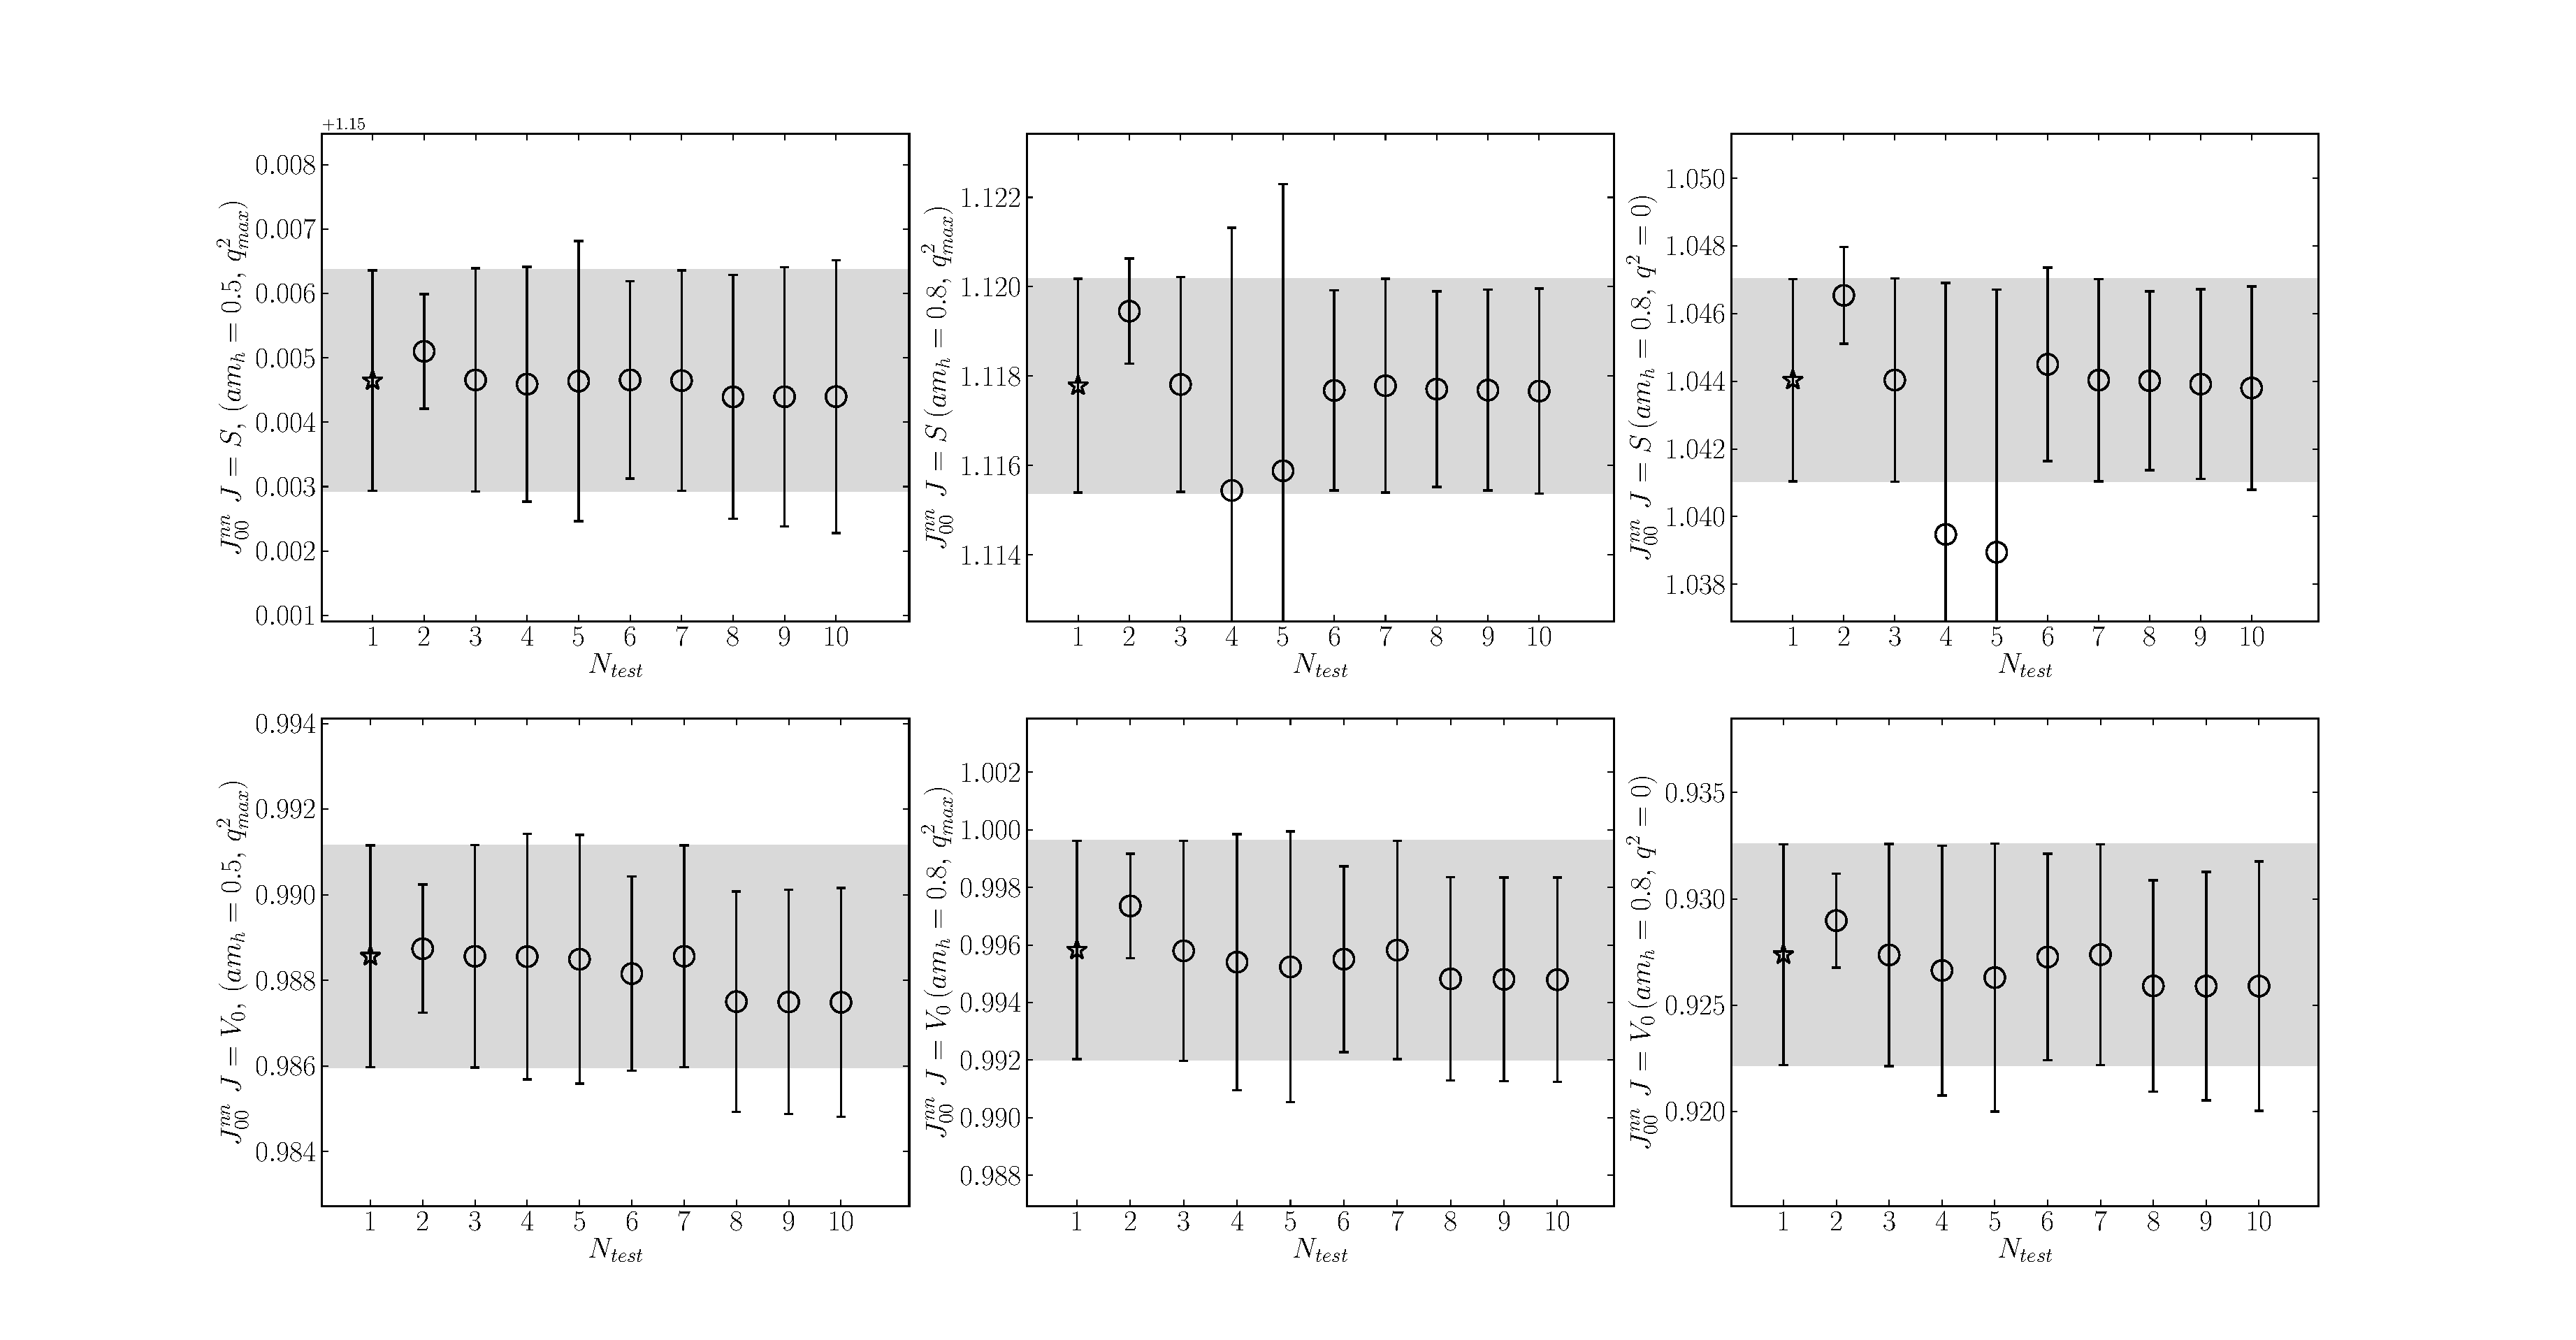
\includegraphics[width=1.4\textwidth]{images/BsDs/finecorr_fittest.pdf}
    \caption{Tests on the correlator fits on the fine ensemble. $N_{\text{test}}=1$ gives the final accepted result. $N_{\text{test}}=2$ and $3$ gives the results of setting $N_{\text{exp}}=4$ and $6$ respectively. $N_{\text{test}}=4$ gives the results when all priors are loosened by 50\%. $N_{\text{test}}=5$ gives the result of setting $t_{\text{cut}}=4$ rather than $2$ for all correlators. $N_{\text{test}}=6$ gives the result without marginalising out the $n=5$ excited state. $N_{\text{test}}=7$ gives the result of moving the svd cut from $10^{-3}$ to $10^{-2}$. $N_{\text{test}}=8,9,10$ gives the result of using a chained fit described above with priors for the full correlated fit given additional fractional errors of 100\%, 150\% and 200\% respectively. \label{fig:corr_tests_BsDs}}
\end{figure}

The stability issue is likely due to the size of the covariance matrix for the data, which must be inverted to estimate $\chi^2$. We took two steps toward mitigating this. The first is to impose an svd-cut. The second step we took was to employ a chained-fitting approach (this was required on the superfine and ultrafine data only). We first performed an array of smaller 'individual' fits, each fitting the correlators relevant only to one $m_h$ and one $|a{\bf{p}}_{D_s}|$ value. In the case of set 4, for example, this results in 11 separate fits. Then, a full simultaneous fit of all of the correlators was carried out, with priors set to the results of the smaller fits. To be conservative we multiplied these priors by $1\pm 1.5$, i.e., the priors end up with over 150\% variance. This both speeds up the full fit and improves the stability of the results. We tested the validity of the results by varying the additional fractional error between 100\% and 200\%, this caused negligible changes in the results. Since we did not need to take this measure on the fine ensemble, we performed both a standard simultaneous fit and chained fits of this type as a check for the chained fits. Tests 8, 9 and 10 on Fig. \ref{fig:corr_tests_BsDs} show the results of these chained fits in comparison to the more traditional fit.

The priors for the 'traditional' fits to fine and fine-physical (sets 2 and 3) data, and individual chained superfine and ultrafine (sets 4 and 5) fits, were set up as follows. We set Gaussian priors for the parameters $J_{jk}$, and log-normal priors for all other parameters. Using log-normal distributions forbids ground state energies $E_0^M$, excited energy differences $E_n^M-E_{n-1}^M$, and amplitudes $a_n^M$ from both becoming negative and moving arbitrarily close to zero, improving the stability of the fit.

Priors for ground state energies log($E_0^M$) and amplitudes log($a_0^M$) are set according to an empirical-Bayes approach, plots of effective energies and amplitudes of the correlation functions are inspected to deduce reasonable priors. The ground-state oscillating parameters log($a_0^{M,o}$), log($E_0^{M,o}$), are given the same priors as the non-oscillating states, with errors inflated by 50\%. The resulting priors always have a variance of at least 10 times that of the final result. The log of oscillating and non-oscillating excited state energies, log($E_i^{M,(o)}-E_{i-1}^{M,(0)}$), $i>0$ are given prior values of log($2\Lambda_{\text{QCD}}\pm \Lambda_{\text{QCD}}$). We set $\Lambda_{\text{QCD}}=0.5$GeV. The excited state amplitudes log($a_i^M$),$i>0$ are given priors of $-1.9\pm 3.3$ for non-oscillating states, and $-3.0\pm 2.0$ for oscillating states. The ground-state non-oscillating to non-oscillating 3-point parameter, $J_{00}^{nn}$ is given a prior of $1\pm 0.5$, and the rest of the 3-point parameters $J_{jk}^{nn}$ are given $0\pm 1$.

The current matrix elements we require can be extracted from the fit parameters via
\begin{align}
  \langle D_s| J | H_s \rangle |_{\text{lat}} = 2 \sqrt{M_{H_s}E_{D_s}} J^{nn}_{00}.
  \label{eq:currentfit}
\end{align}

\begin{figure}[htb!]
  \hspace{-30pt}
    \hspace{-10pt}
    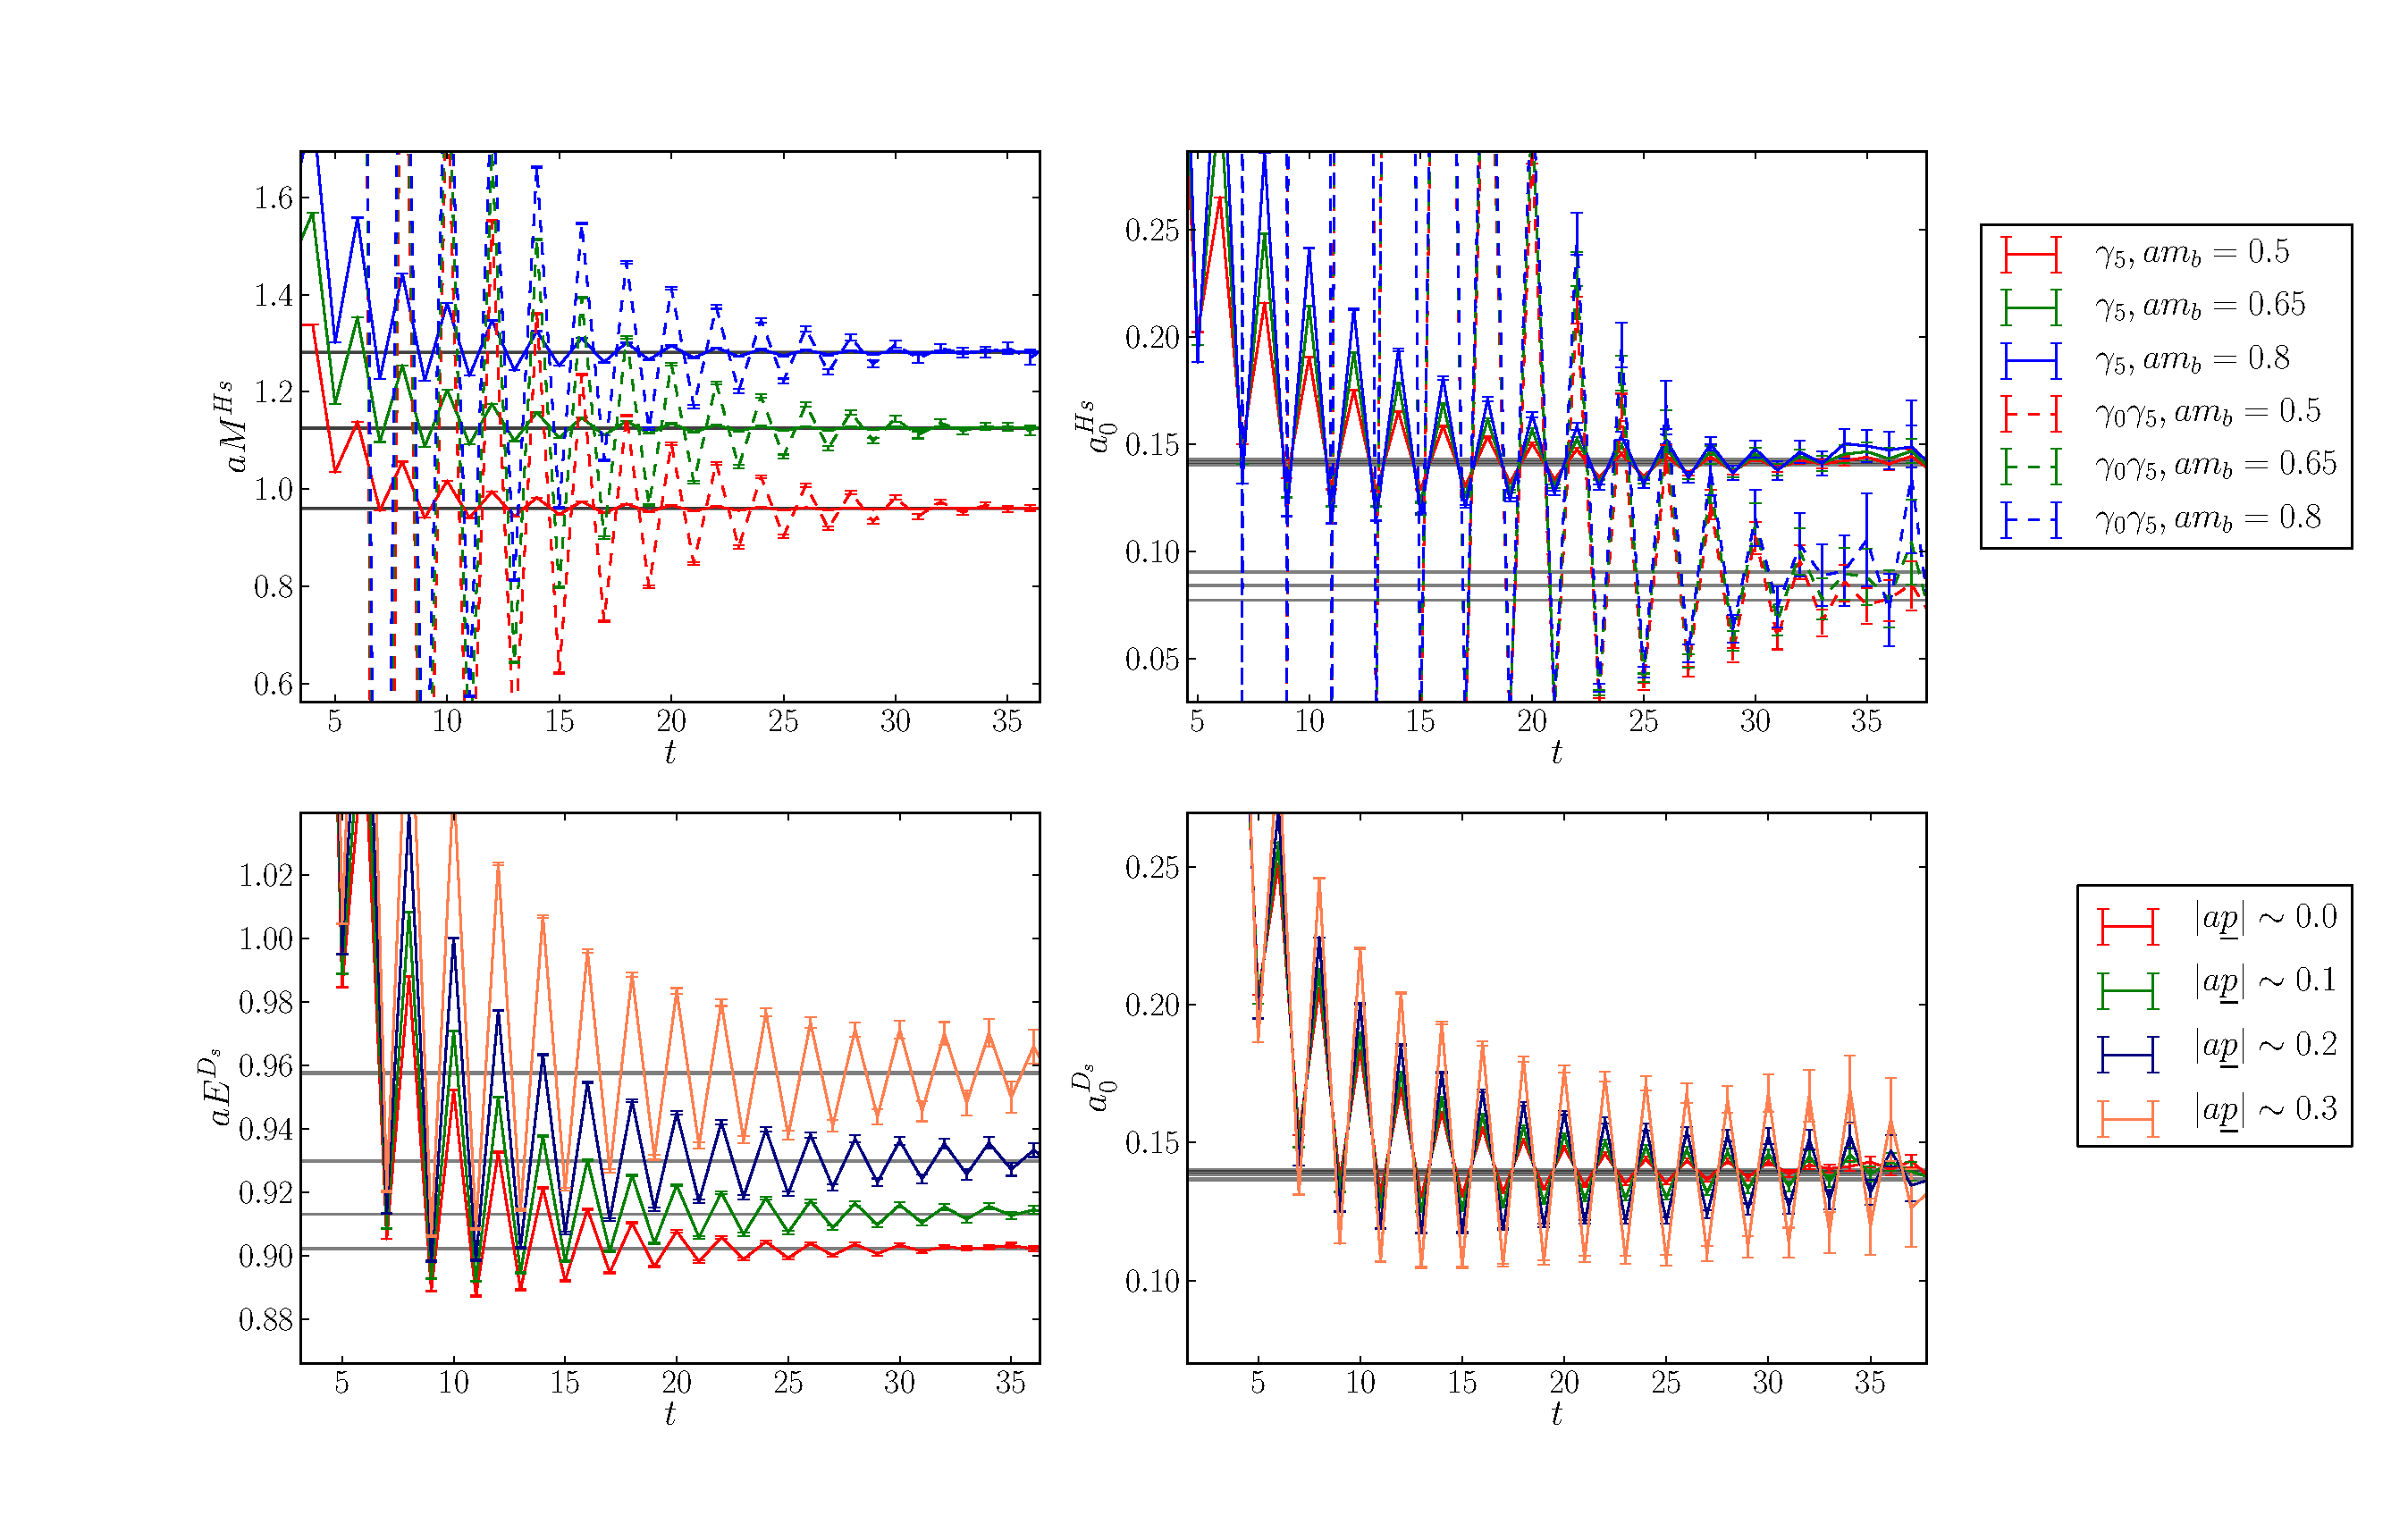
\includegraphics[width=1.2\textwidth]{images/BsDs/fine_2pt_summary.pdf}
    \caption{
Superaveraged effective energies (given by Eq. \eqref{eq:effectivemass}) and amplitudes (given by Eq. \eqref{eq:effectiveamp}) for a selection of 2-point correlators on the fine ensemble. The grey bands show the corresponding results for these quantities from the simultaneous Bayesian fits. These plots supply a further check of our correlator fits - results of the Bayesian fits are in good agreement with the effective energies and amplitudes.  \label{fig:2ptcorrs_BsDs}}
\end{figure}

\begin{figure}[htb!]
    \hspace{-60pt}
    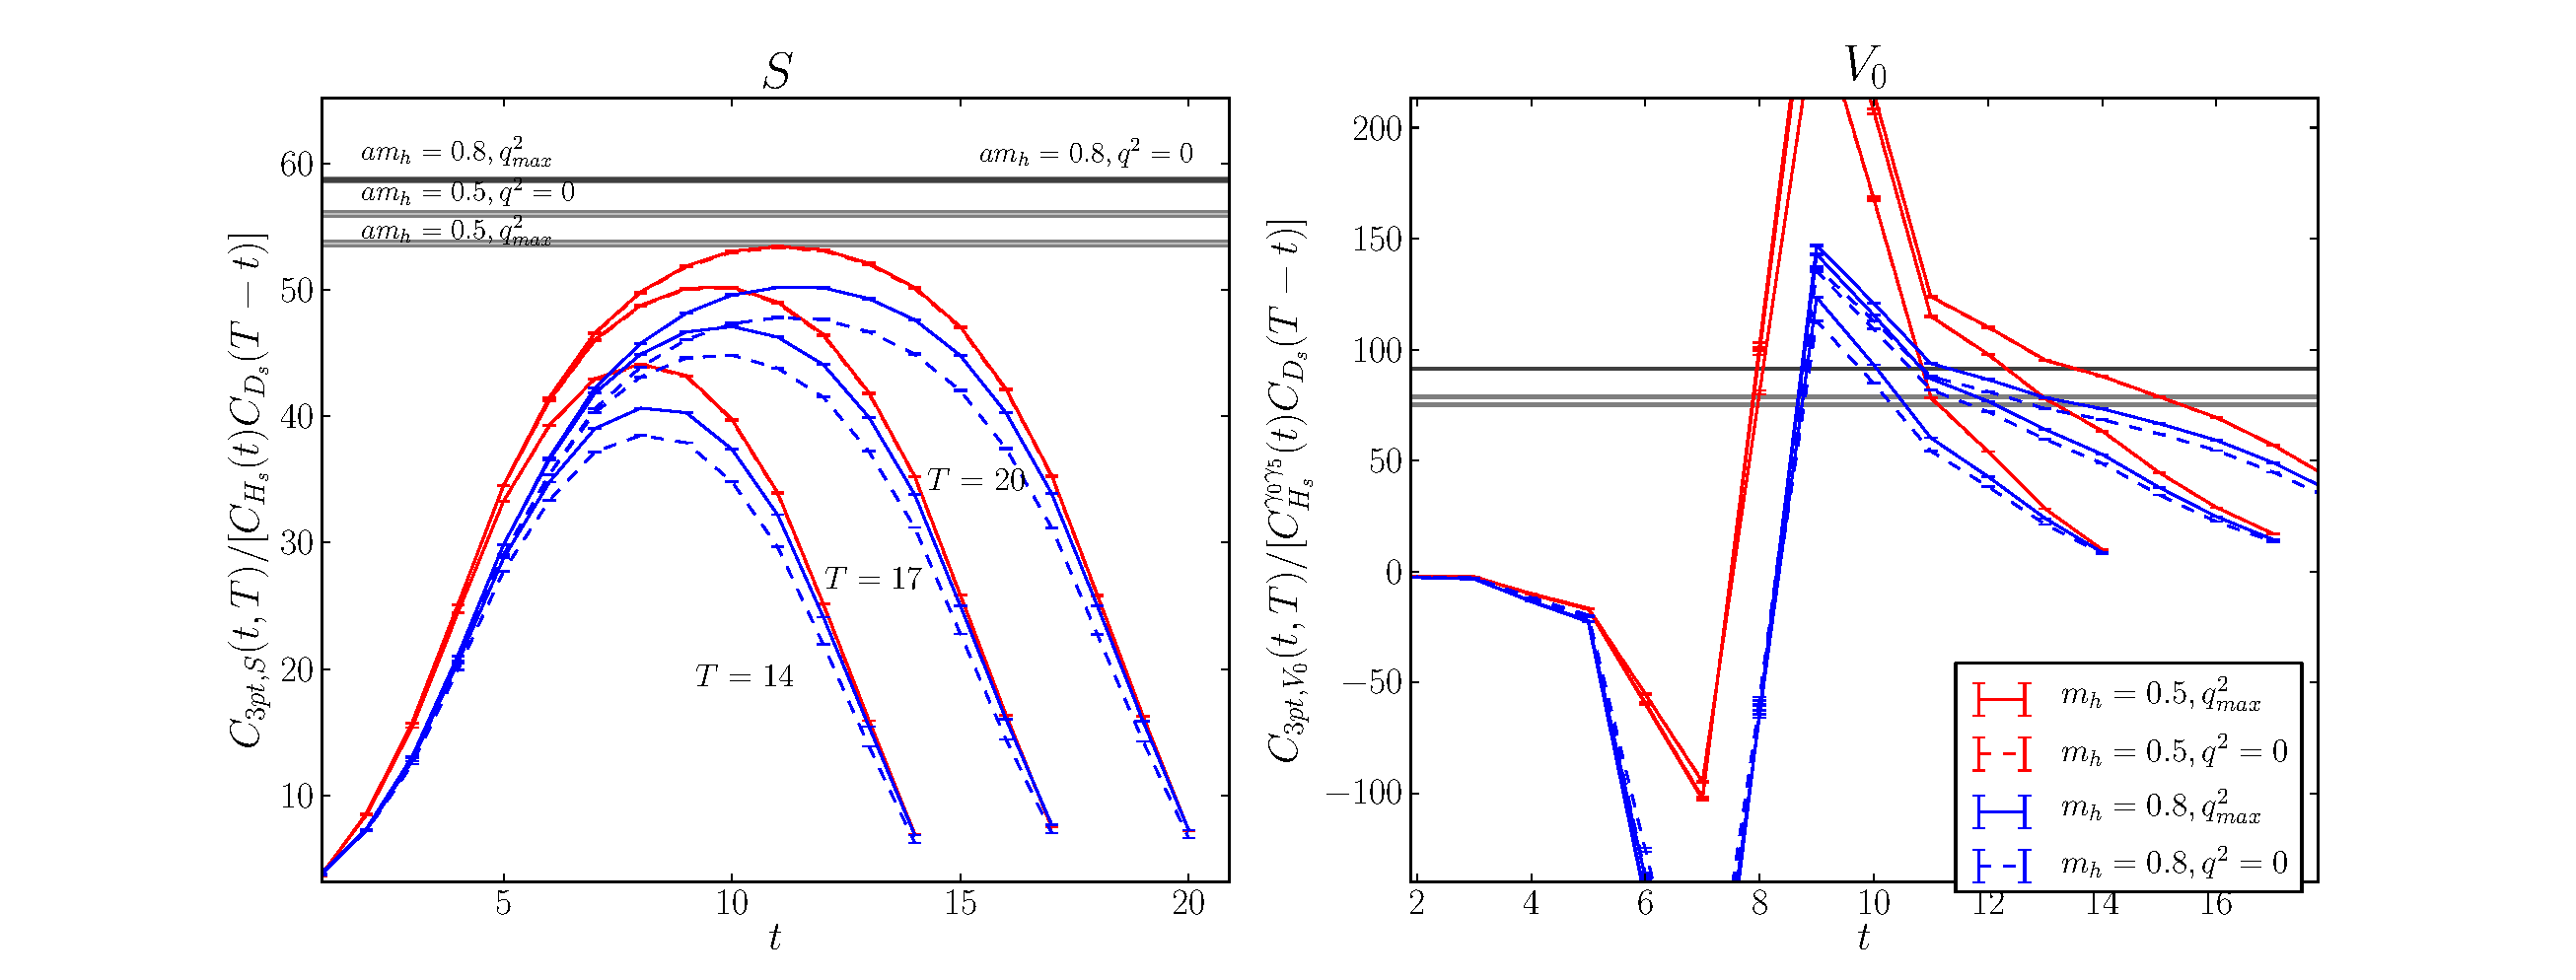
\includegraphics[width=1.3\textwidth]{images/BsDs/fine_3pt_summary.pdf}
    \caption{$\tilde{C}_3(t,T)/\tilde{C}^{H_s}(t) \tilde{C}^{D_s}(T-t)$, which should plateau at $J_{00}^{nn}$, in the fine ensemble for the $J=S$ and $J=V_0$ cases. The grey bands show the corresponding results for these quantities from the simultaneous Bayesian fits. Unfortunately, in the $V_0$ case the oscillating component dominates the correlation function, preventing any plateau from being visible. \label{fig:3ptcorrs_BsDs}}
\end{figure}

\subsection{Vector Current Renormalization}

In HISQ, the local scalar current $(1\otimes 1)$ (multiplied by the mass difference of flavours it is charged under) requires no renormalization due to its connection to the partially conserved vector current through the PCVC relation. This is not the case for the local temporal vector current $(\gamma_0\otimes \gamma_0)$. The partially conserved vector current is a complicated linear combination of many local and point-split lattice currents. In this calculation we use only the local part of the vector current, this improves the statistics of our results but creates the need for the resulting current matrix element to be multiplied by a matching factor $Z_V$ to produce the appropriate continuum current. We found $Z_V$ via a fully non-perturbative method \cite{Koponen:2013tua}.

When both meson states in the matrix elements are at rest (the zero recoil point), the scalar and local vector matrix elements are related via the PCVC relation:
\begin{align}
  ( M_{H_s}& - M_{D_s} ) Z_V \langle D_s | V_0 | \hat{H}_s \rangle|_{\text{lat}}(q^2_{\text{max}}) = (m^{\text{val}}_{h0} - m^{\text{val}}_{c0}) \langle D_s | S | H_s \rangle|_{\text{lat}}(q^2_{\text{max}}).
  \label{eq:ward}
\end{align}
$Z_V$ can be extracted from this relation since the matrix elements are already computed as part of the calculation. Our calculation is self-renormalizing, in the sense that the normalization can be found at no extra computational cost. The $Z_V$ values found on each ensemble and $am^{\text{val}}_{h0}$ are given in Table \ref{tab:norms}.

We also removed tree-level mass-dependent discretization effects using a normalization constant $Z_{\text{disc}}$ defined in Eq. \eqref{eq:Zdisc}.

Combining these normalizations with the lattice current from the correlation function fits, we found values for the form factors at a given heavy mass, lattice spacing, and $q^2$:
\begin{align}
  \nonumber
  f_0^s&(q^2) = {m^{\text{val}}_{h0} - m^{\text{val}}_{c0}\over M_{H_s}^2 - M_{D_s}^2 } Z_{\text{disc}} \langle D_s | S | H_s \rangle|_{\text{lat}}(q^2) \\
  \label{eq:normalizations}
  f_+^s&(q^2) = {Z_{\text{disc}} \over 2M_{H_s}} \times \\ \nonumber &{ \delta^M \langle D_s | S | B_s \rangle|_{\text{lat}}(q^2) - q^2 Z_V \langle D_s | V_0 | B_s \rangle|_{\text{lat}}(q^2) \over {\bf{p}}^2_{D_s}}.
\end{align}
I have here explicitly denoted the dependence of the matrix elements on $q^2$ as a reminder that the matrix elements have $q^2$ dependence via the $D_s$ momentum.

\begin{table}
\begin{center}
\begin{tabular}{ c c c c }
\hline
Set & $am_h^{\text{val}}$ & $Z_V$& $Z_{\text{disc}}$\\ [0.5ex]
\hline
0 & 0.5 & 1.0151(32) & 0.99819\\ [0.5ex] 
 & 0.65 & 1.0240(37) & 0.99635\\ [0.5ex] 
 & 0.8 & 1.0368(49) & 0.99305\\ [0.5ex] 
\hline
1 & 0.5 & 1.0134(24) & 0.99829\\ [0.5ex] 
 & 0.8 & 1.0348(29) & 0.99315\\ [0.5ex] 
\hline
2 & 0.427 & 1.0027(25) & 0.99931\\ [0.5ex] 
 & 0.525 & 1.0059(29) & 0.99859\\ [0.5ex] 
 & 0.65 & 1.0108(37) & 0.99697\\ [0.5ex] 
 & 0.8 & 1.0197(49) & 0.99367\\ [0.5ex] 
\hline
3 & 0.5 & 1.0037(40) & 0.99889\\ [0.5ex] 
 & 0.65 & 1.0087(46) & 0.99704\\ [0.5ex] 
 & 0.8 & 1.0160(53) & 0.99375\\ [0.5ex] 
\hline
\end{tabular}
    \caption{Normalization constants applied to the lattice axial vector current in \eqref{eq:normalizations}. $Z_V$ is found from \eqref{eq:ward} and $Z_{\text{disc}}$ from \eqref{eq:Zdisc}. \label{tab:norms}}
\end{center}
\end{table}

\subsection{Extrapolation to the Physical Point}
\label{sec:extrapolation}

We now address the extrapolation of the $f_{0}^s(q^2)$ and $f_{+}^s(q^2)$ values to continuum, physical quark masses and arbitrary $q^2$. We took two complementary approaches to the extrapolation.

One we refer to as the {\textit{ratio}} approach, in which one extrapolates the quantity
\begin{align}
  R^s_{0,+}(q^2) \equiv {f^s_{0,+}(q^2)\over f_{H_c}\sqrt{M_{H_c}}}\,.
  \label{eq:ratio}
\end{align}
to the physical point. Discretisation effects appear to cancel to a large extent in this ratio, resulting in a better controlled continuum extrapolation. The value at the physical point is then multiplied by $f_{B_c}\sqrt{M_{B_c}}$ to isolate the form factors, where we find $f_{B_c}$ via a separate extrapolation (detailed in Sec. \ref{sec:stability_BsDsstar}), and take the PDG value for $M_{B_c}$ \cite{PhysRevD.98.030001}. While this approach improves the continuum extrapolation, it has the downside of introducing errors from scale-setting on account of $R_{0,+}^s(q^2)$ being dimensionful quantities (as opposed to $f^s_{0,+}(q^2)$ which are dimensionless).

In the other method, that we refer to as the {\textit{direct}} approach, one simply extrapolates the form factors to the physical point. The form factors by themselves have larger discretisation effects than $R_{0,+}^s(q^2)$, but since $f^s_{0,+}$ are dimensionless, the results are insensitive to scale-setting uncertainty.

We use identical fit functions for both approaches. In the below discussion, we use the notation $F^s_{0,+}(q^2)$ to denote either $f^s_{0,+}(q^2)$ or $R_{0,+}^s(q^2)$, depending on the approach being applied.

\subsubsection{Kinematic Behaviour}

Our fit form for the extrapolation is a modified version of the Bourrely-Caprini-Lellouch (BCL) parameterisation for pseudoscalar-to-pseudoscalar form factors \cite{Bourrely:2008za}:
\begin{align}
  \label{eq:BCL}
  &F^s_0(q^2)|_{\text{fit}} = {1\over 1 - {q^2\over M_{H_c^0}^2} } \sum_{n=0}^{N-1} a_n^0 z^n(q^2), \\
  &F^s_+(q^2)|_{\text{fit}} = {1\over 1 - {q^2\over M_{H_c^*}^2} } \sum_{n=0}^{N-1} a_n^+ \left( z^n(q^2) - {n\over N} (-1)^{n-N} z^N(q^2) \right). \nonumber
\end{align}
The functon $z(q^2)$ maps $q^2$ to a small region inside the unit circle on the complex $q^2$ plane, defined by
\begin{align}
  z(q^2) = {\sqrt{t_+ - q^2} - \sqrt{t_+ - t_0} \over \sqrt{t_+ - q^2} + \sqrt{t_+ - t_0} },
\end{align}
where $t_+ = (M_{H_s}+M_{D_s})^2$, and we choose $t_0$ to be $t_0 = 0$. This $t_0$ choice means that at $q^2=0$ the fit functions simplify to $F_{0,+}^s(0) = a_0^{0,+}$. Throughout the physical range of $q^2$, $z$ is restricted to the range $0<z<0.06$, resulting in a fast converging series in powers of $z$. We truncate at $N=3$, adding further orders of $z^n$ does not affect the results of the fit.

The factors in front of the sums in the BCL parameterisation account for subthreshold poles in the form factors due to the production of on-shell $H_{c0}$ and $H_c^*$ states in the crossed channel of the semileptonic decay.

To estimate $M_{H_{c0}}$, the scalar heavy-charm meson mass, at each of the heavy masses we use, we leveraged the fact that the splitting $\Delta_0 = M_{H_{c0}} - M_{H_c}$ is due to an orbital excitation and therefore independent of the heavy quark mass. This has been calculated in \cite{Dowdall:2012ab} to be $\Delta_0 = 0.429(13)$GeV. Combined with an $H_c$ mass from our correlators, we can construct the $H_{c0}$ mass: $M_{H_{c0}} = M_{H_c} + \Delta_0$. We did not take the error on $\Delta_0$ into account in the fit since the precise position of the pole has a small effect on the fit results.

To estimate $M_{H^*_c}$, the vector heavy-charm mass, we use the fact that the splitting $ M_{H_c^*} - M_{H_c}$ vanishes in the infinite heavy mass limit. $M_{H_c^*}$ then takes the approximate form $M_{H_c^*} \simeq M_{H_c} + \order{1/m_h}$. To reproduce this behaviour we use the ansatz $M_{H_c^*} = M_{H_c} + x/M_{\eta_h}$, and fix $x$ at the physical point to find $x=0.508$GeV$^2$. To do this we use the result $M_{B_c^*}-M_{B_c}=54\,$MeV from \cite{Dowdall:2012ab}.

\subsubsection{Heavy Mass and Discretisation Effects}

To account for variation in heavy mass and discretisation effects in a general way, we gave the following form to each of the $a_n^{0,+}$ coefficients:
\begin{align}
  \nonumber  a_n^{0,+} = & \,\,\left( 1 + \rho^{0,+}_n \text{log}\left(M_{\eta_c}\over M_{\eta_h}\right)\right) \times \\ \nonumber
  &\sum_{i,j,k = 0}^{2,2,2} d^{0,+}_{ijkn} \left({2\Lambda_{\text{QCD}}\over M_{\eta_h} }\right)^{i} \left({ am^{\text{val}}_{h0} \over \pi }\right)^{2j} \left({ aE_{D_s} \over \pi }\right)^{2k} \\ &\times\left(1 + \mathcal{N}_{\text{mistuning},n}^{0,+} \right)\,.
      \label{eq:mhfitfun}
\end{align}

To understand this form, focus first on the sum. Powers of $(2\Lambda_{\text{QCD}}/M_{\eta_h})$ give an HQET inspired way of quantifying the variation in the results due to the changing heavy mass. $M_{\eta_h}$ varies strongly and monotonically with the heavy quark mass, so acts as a suitable proxy. $\Lambda_{\text{QCD}}$ is the confinement scale, which we set to 0.5GeV.

The two scales expected to be the largest sources of discretisation effects are the heavy mass $am_{h0}^{\text{val}}$, and the energy in the $D_s$ meson, $aE_{D_s}$, especially when it is given a large spatial momentum. Adding further, smaller scales, like $a\Lambda_{\text{QCD}}$, had no effect on the results.

The coefficients $d^{0,+}_{ijkn}$ are fit parameters given prior distributions of $0\pm 2$. In the ratio case, these carry mass dimension GeV$^{-3/2}$, hence this prior corresponds to a prior of $0\pm (2\Lambda_{\text{QCD}})^{-3/2}$.

To account for any required matching between HQET and QCD, we included a log term in front of the sum. $\rho^{0,+}_n$ are fit parameters with prior distribution $0\pm 1$.

The fact that $f^s_+(0) = f^s_0(0) \,(\,\Rightarrow a^+_0 = a^0_0)$ is a very powerful constraint within the heavy-HISQ approach. Since this must be true at all $m_h$, this translates to constraints in the fit parameters: $d^+_{i000}=d^0_{i000} \,\forall \,i$ and $\rho^+_0 = \rho^0_0$. We imposed these constraints in the fit, which serve to stablize the heavy mass extrapolation.

\subsubsection{Mass Mistunings}

We dealt with possible mistuning in the $c$, $s$ and $l$ masses in the same way as in the $B_s\to D_s^*$ study. We included the terms $\mathcal{N}_{\text{mistuning},n}^{0,+}$ in each $a^{0,+}_n$ coefficient, given by
\begin{align}
  \mathcal{N}_{\text{mistuning},n} &= {c_{s,n}^{\text{val}} \delta^{\text{val}}_s + c_{s,n} \delta_s + 2 c_{l,n} \delta_l \over 10 m_s^{\text{tuned}} }
    \label{eq:mistuning}
  +c_{c,n}^{0,+} \left({ M_{\eta_c} - M_{\eta_c}^{\text{phys}} \over M_{\eta_c}^{\text{phys}}}\right)\,,
\end{align}
where $c^{0,+}_{l,n}$, $c^{0,+}_s$ and $c^{0,+}_{ci}$ are fit parameters with prior distributions $0\pm 1$. $\delta_{s,l}^{(\text{val})}$ are defined in Sec. \ref{sec:mistuning_BsDsstar} and $m_s^{\text{tuned}}$ is defined in Eq. \eqref{eq:strange_mistuning}.

%% The strange mistuning is accounted for here using an approach first used in \cite{Chakraborty:2014aca}. We define the term $\delta_s = m^{\text{val}}_{s0} - m_s^{\text{tuned}}$, where $m_s^{\text{tuned}}$ is defined by
%% \begin{align}
%%   m_s^{\text{tuned}} = m^{\text{val}}_{s0} \left({ M^{\text{phys}}_{\eta_s} \over M_{\eta_s} }\right)^2.
%% \end{align}
%% $M_{\eta_s}^{\text{phys}}$ was determined in a lattice simulation from the masses of the pion and kaon \cite{Dowdall:2013rya}.

%% We similarly account for (sea) light quark mistuning by defining $\delta_l = m_{l0} - m_l^{\text{tuned}}$. We find $m_l^{\text{tuned}}$ from $m_s^{\text{tuned}}$, using the fact that the ratio of quark masses is regularization independent, and was calculated in \cite{Bazavov:2014wgs}:
%% \begin{align}
%%   \left.\frac{m_s}{m_l}\right\rvert_{\textrm{phys}} = 27.18(10).
%% \end{align}
%% We set $m_l^{\text{tuned}}$ to $m_s^{\text{tuned}}$ divided by this ratio.

All higher order contributions, like $\delta^{(\text{val})\,2}_{s,l}$ or $(M_{\eta_c}-M_{\eta_c}^{\text{phys}})^2$ are too small to be resolved by our lattice data, so are not included in the fit.

\subsubsection{Negligable Effects}

Finite volume effects are negligible in our calculation, we do not include any associated error. Finite volume corrections to the $B\to Dl\nu$ form factors in chiral perturbation theory were calculated in \cite{Laiho:2005ue}. They found the $B\to Dl\nu$ form factor at zero recoil, with a lattice size of $L=2.5$fm, and pion mass equal to or greater than physical, never exceeded $10^{-4}$. There is no reason to believe changing the spectator quark from light to strange, and moving away from zero recoil, will increase this effect.

In our simulation we set $m_u=m_d\equiv m_l$, this means our results do not account for isospin breaking. By moving the $m_l^{\text{tuned}}$ value up and down by the PDG value for $m_d-m_u$, we tested for any signs of isospin breaking having an effect on the results. The resulting effect was negligible in comparison to all other sources of error.

Since we take the physical result at $M_{\eta_h}=M_{\eta_b}$, the uncertainty in $M_{\eta_b}$ will contribute an uncertainty in the final result. We use the PDG result for $M_{\eta_h}$ \cite{PhysRevD.98.030001}. However, $\bar{b}-b$ annihilation and electroweak corrections make this somewhat different to the appropriate value on the lattice. We estimate the corresponding uncertainty in $M_{\eta_b}$ to be no greater than $\pm10$MeV. To see how this changes the result of the extrapolation, we varied $M_{\eta_b}$ up and down by 10MeV and studied how our result at $f_0(q^2_{\text{max}})$ changes. The change is never greater than $10^{-4}$, which is negligible in comparison to the other errors.

\section{Results}
\label{sec:results}

Tables \ref{tab:masses} and \ref{tab:kinetic} in Sec. \ref{sec:tables} give numerical values for the form factors, the ratios $R_{0,+}^s(q^2)$, and parameters extracted from the correlation function fits required for the extrapolations to the physical point.

I will first show results from the ratio method, then the direct method. In both cases, we performed a simpler fit at zero recoil first, then a larger fit taking into account all data throughout $q^2$.  In each case, our results are statistics dominated. The results from the two methods are in good agreement.

\subsection{Ratio Method}
\label{sec:ratiomethod}

\subsubsection{Zero Recoil}

\begin{figure}[htb!]
  \begin{center}
  \hspace{-10pt}
  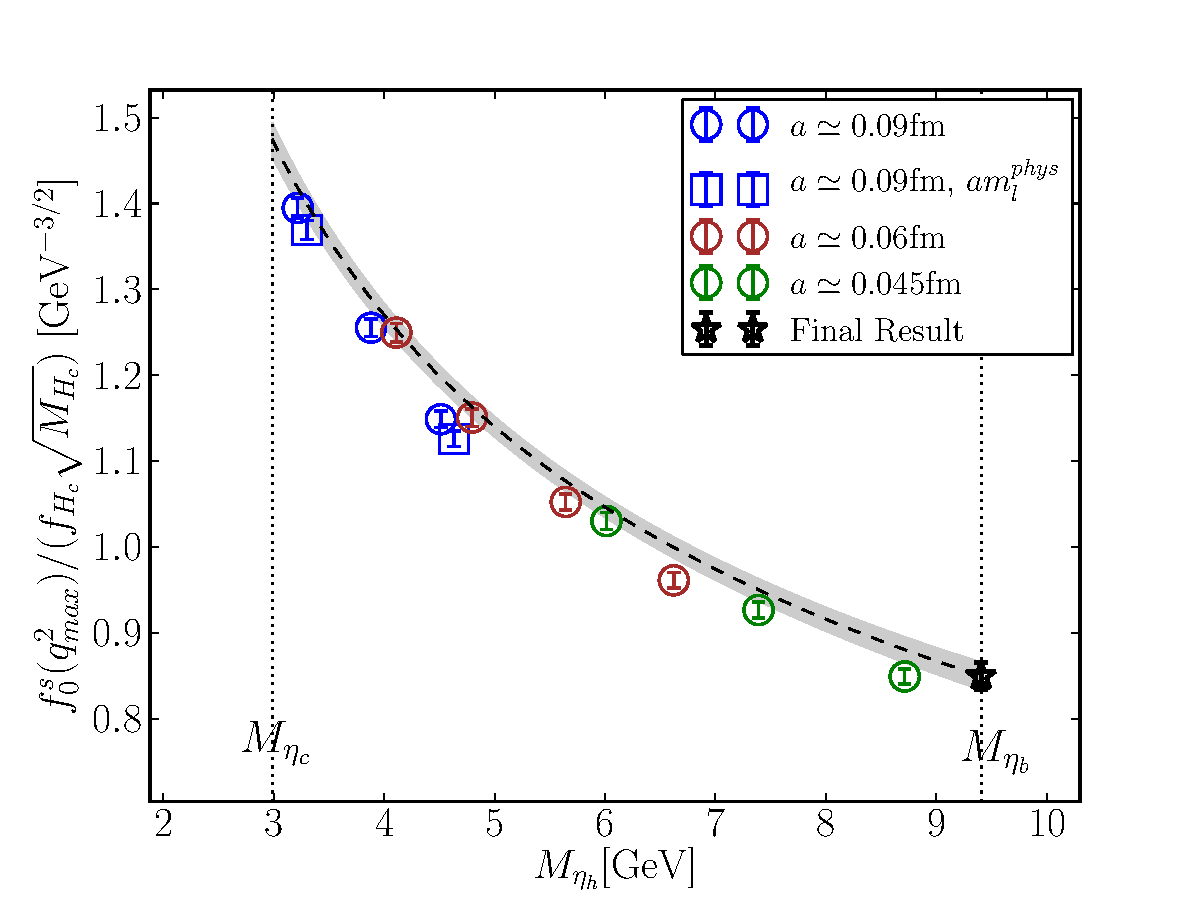
\includegraphics[width=0.85\textwidth]{images/BsDs/ratio/f0fHc_vsmh.pdf}
  \caption{ $R_0^s(q^2_{\text{max}}) = f_0^s(q^2_{\text{max}})/(f_{H_c}\sqrt{M_{H_c}})$ against $M_{\eta_h}$ (a proxy for the heavy quark mass). The grey band shows the result of the extrapolation at $a=0$ and physical $l$,$s$ and $c$ masses. Sets listed in the legend follow the order of sets in table \ref{tab:ensembles}. \label{fig:ratioq2max}}
    \end{center}
\end{figure}

We performed an isolated extrapolation of $R^s_0(q^2_{\text{max}})$ to the physical point. To do this we used a simplified fit form for $R^s_0(q^2_{\text{max}})$ consisting of the right hand side of \eqref{eq:mhfitfun},with the index $n$ discarded.
We find
\begin{align}
  R_0^s(q^2_{\text{max}}) = {f_0^s(q^2_{\text{max}})\over f_{B_c}\sqrt{M_{B_c}}} = 0.843(18) \text{GeV}^{-3/2}\,.
\end{align}
The extrapolation against $M_{\eta_h}$ is illustrated in Fig. \ref{fig:ratioq2max}. As can be seen here, data for this ratio has a very weak dependence on the lattice spacing. The error budget for this result is given in Table \ref{ratioq2max_budget}.

\begin{table}[htb!]
  \begin{center}
    \begin{tabular}{c c}
      \hline
      Source & \% Fractional Error \\ [0.5ex]
      \hline
      Statistics & 1.72  \\ [1ex]
      Scale Setting & 1.35  \\ [1ex]
      $m_h \to m_b$, & 0.87  \\ [1ex]
      $a\to 0$ & 0.16  \\ [1ex]
      mistuning & 0.72 \\ [1ex]
      \hline
      Total & 2.16 \\ [1ex]
      \hline
    \end{tabular}
  \end{center}
  \caption{Error budget for $R_0^s(q^2_{\text{max}})$. \label{ratioq2max_budget}}
\end{table}

We performed a number of tests on this zero recoil extrapolation to test the stability of our fit form, results are given in Fig. \ref{fig:ratiotests}.

\begin{figure}[htb!]
  \begin{center}
  \hspace{-20pt}
  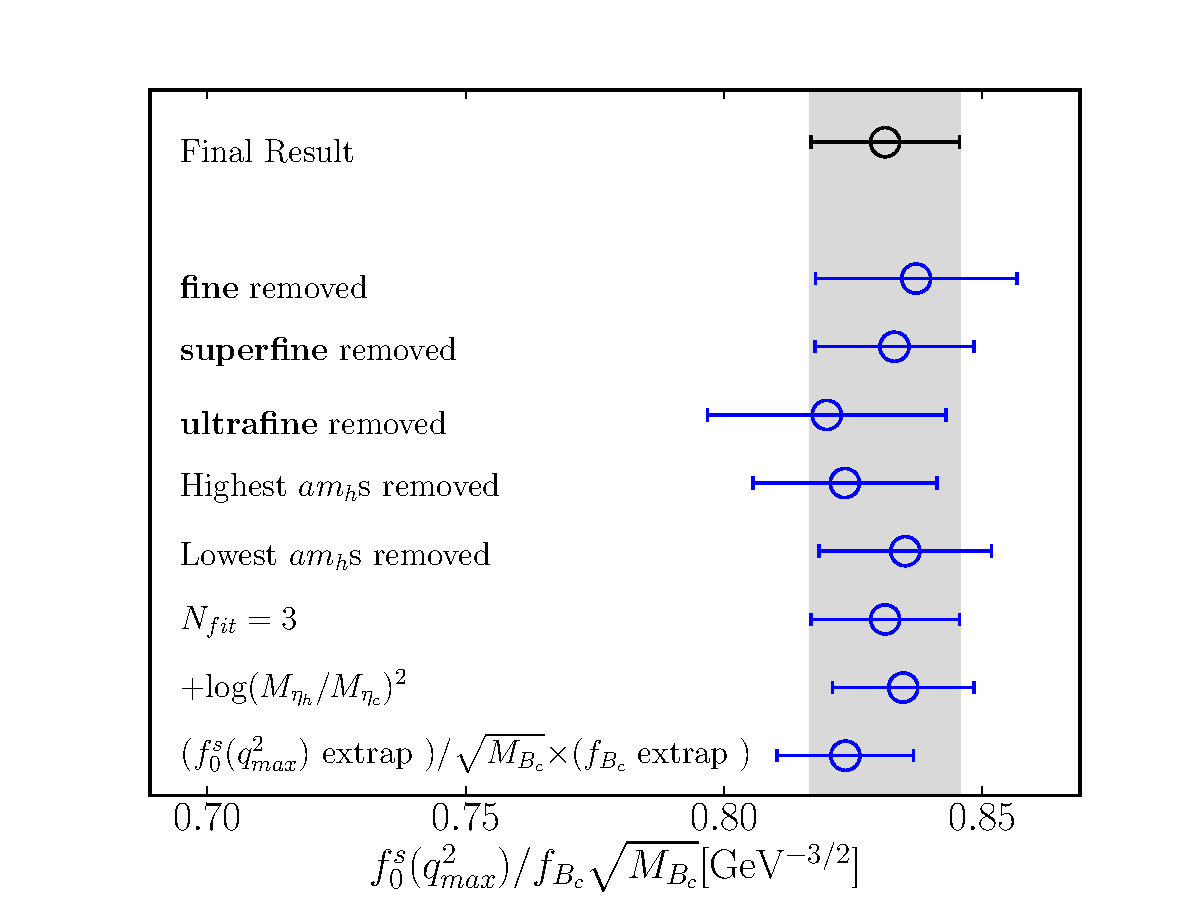
\includegraphics[width=0.85\textwidth]{images/BsDs/ratio/f0dcq2max_stability.pdf}
  \caption{ Results of tests of the $R_0^s(q^2_{\text{max}})$ extrapolation. The top three blue points show $R_0^s(q^2_{\text{max}})$ at continuum and physical $b$ mass, if data from the fine, superfine or ultrafine ensembles are not used in the fit. The fourth and fifth blue points show the result if data at the highest/lowest $am_{h0}^{\text{val}}$ value on each ensemble are removed. The point labelled $N_{fit}=3$ is the result of extending the sum in \eqref{eq:mhfitfun} such that it truncates at 3 rather than 2 in each of the $i,j,k$ directions. The point labelled $+\text{log}(M_{\eta_h}/M_{\eta_c})^2$ represents the result of adding a $\rho_{2,\,n} \text{log}(M_{\eta_h}/M_{\eta_c})^2$ term in the first set of brackets in \eqref{eq:mhfitfun}, where $\rho_{2,\,n}$ are new fit parameters with the same prior distributions as $\rho_{n}$. Similarly $+\text{log}(M_{\eta_h}/M_{\eta_c})/M_{\eta_h}$ shows the result of adding this term multiplied by $\rho_{2,\,n}$. The lowest point shows the result of our direct extrapolation of $f_0^s(q^2_{\text{max}})$ to the physical point, divided by the PDG value for $\sqrt{M_{B_c}}$ \cite{PhysRevD.98.030001} and the result of our extrapolation of $f_{B_c}$ to the physical point detailed in Sec. \ref{sec:stability_BsDsstar}.
    \label{fig:ratiotests}}
  \end{center}
\end{figure}

\subsubsection{Non-zero Recoil}

\begin{figure}[htb!]
  \hspace{-85pt}
  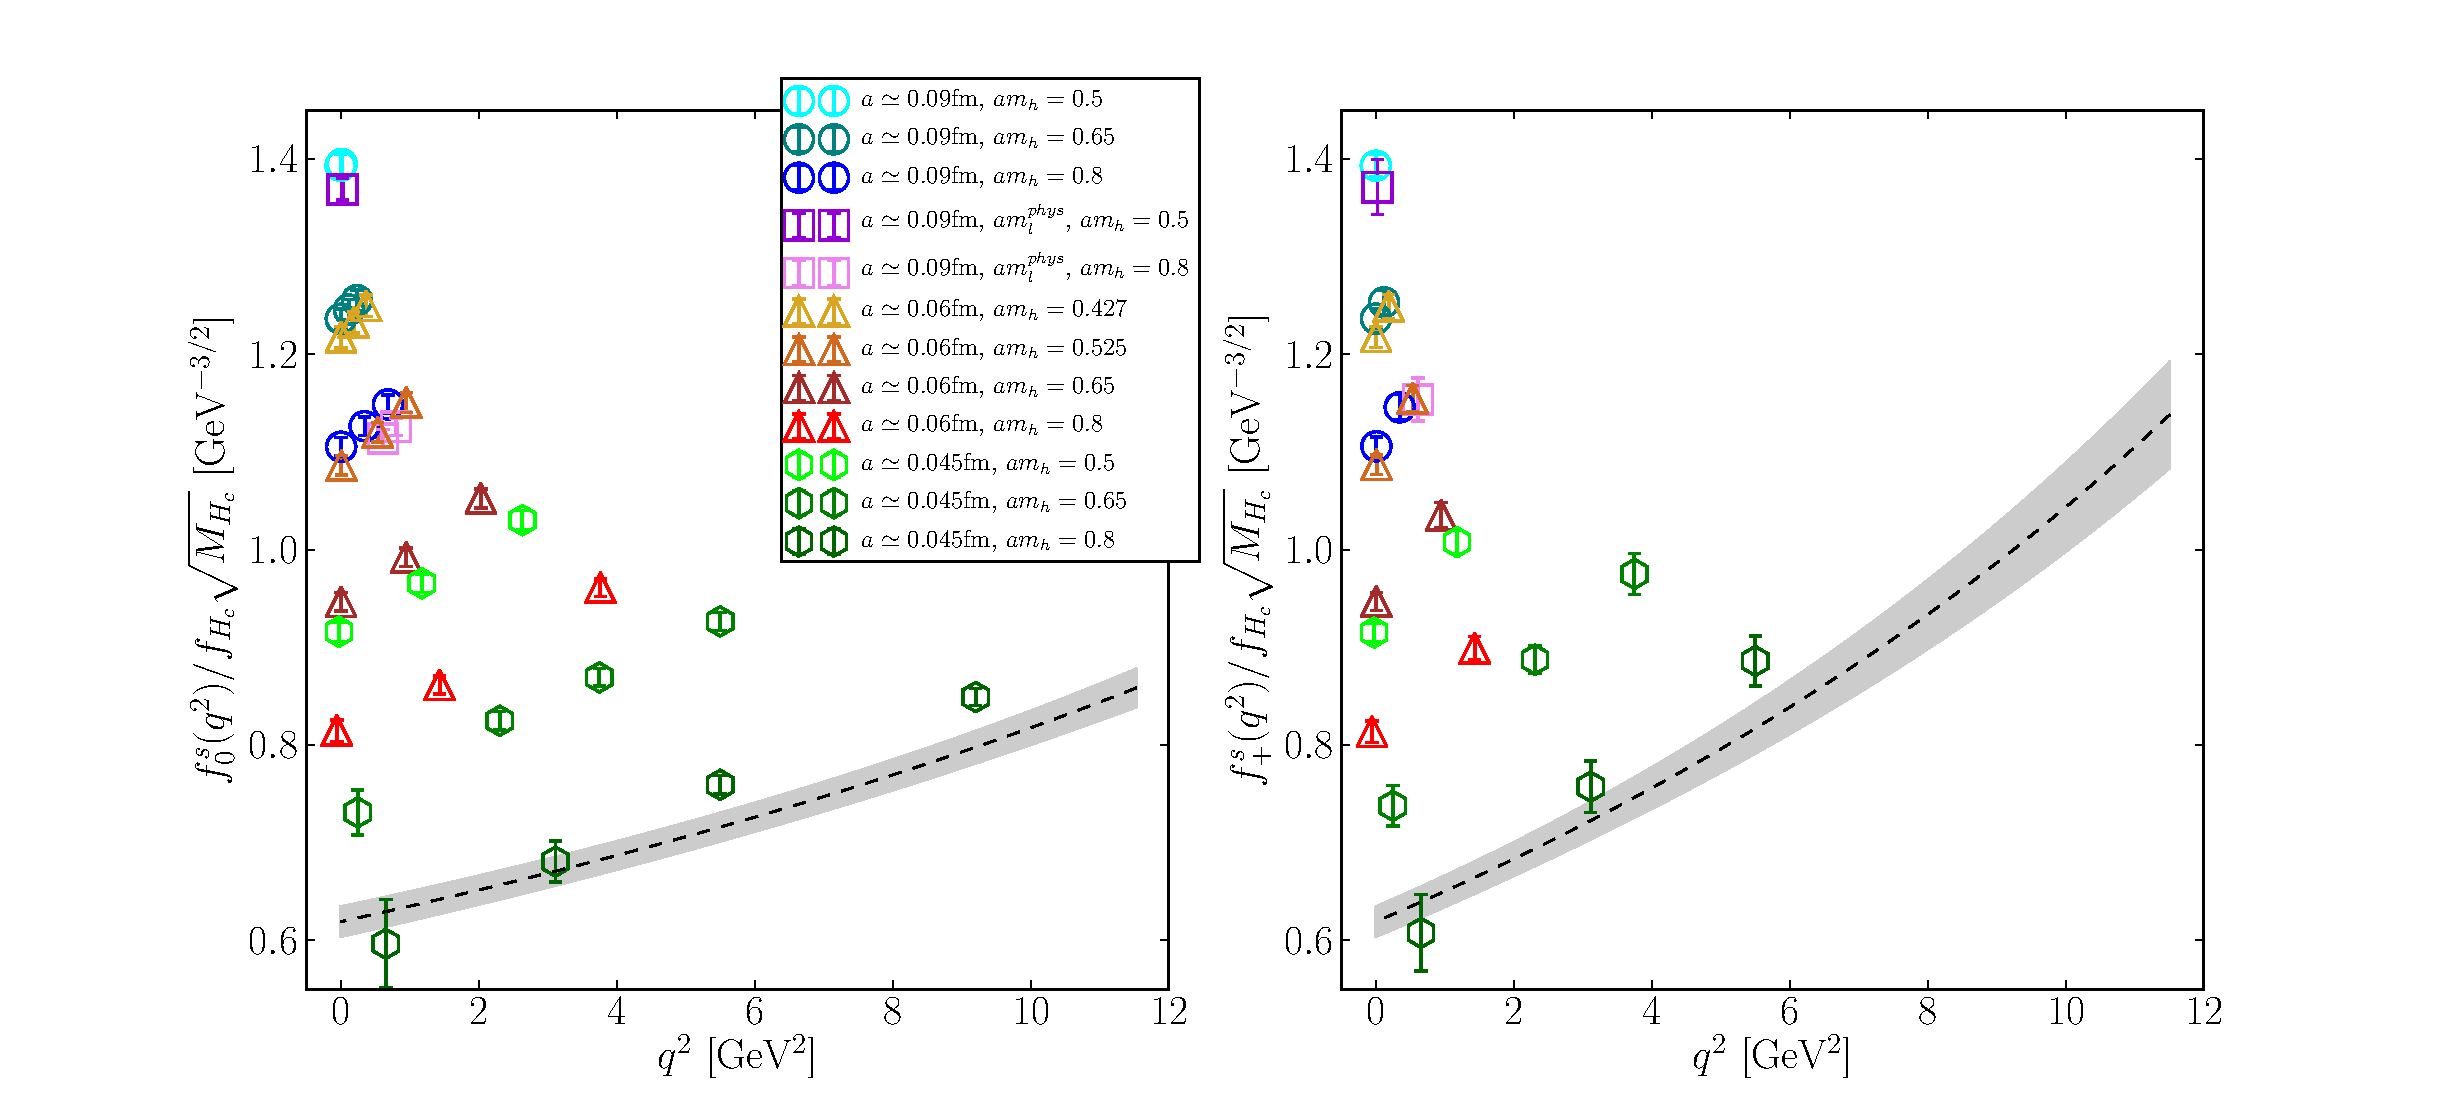
\includegraphics[width=1.50\textwidth]{images/BsDs/ratio/f0fpfHc_vsq2.pdf}
  \caption{ $R_{0,+}^s(q^2) = f_{0,+}^s(q^2)/(f_{H_c}\sqrt{M_{H_c}})$ against $q^2$. The grey band shows the result of the extrapolation at $a=0$ and physical quark masses. Sets listed in the legend follow the order of sets in table \ref{tab:ensembles}. \label{fig:ratiodata}}
\end{figure}

Fig. \ref{fig:ratiodata} shows the result of the full extrapolation of $R_{0,+}^s(q^2)$ throughout the $q^2$ range described in Sec. \ref{sec:extrapolation}. As the heavy mass increases, the $q^2$ range, $0 < (M_{H_s}-M_{D_s})^2$ expands.

To isolate the form factors, the resulting functions $R_{0,+}^s(q^2)$ were multiplied by $\sqrt{M_{B_c}}$ (using the PDG value) and $f_{B_c}$ from our determination detailed in Sec. \ref{sec:stability_BsDsstar}. The resulting form factors are shown in Fig. \ref{fig:ratiovsdirect}, against the form factors found via the direct method.

\subsection{Direct Method}

\subsubsection{Zero Recoil}
\label{sec:directq2max}

\begin{figure}[htb!]
  \begin{center}
  \hspace{-10pt}
  \includegraphics[width=0.85\textwidth]{images/BsDs/direct/f0q2max_vsmh.pdf}
  \caption{ $f_0^s(q^2_{\text{max}})$ against $M_{\eta_h}$ (a proxy for the heavy quark mass). The grey band shows the result of the extrapolation at $a=0$ and physical quark masses. We also include the result from a previous lattice calculation, which used the NRQCD discretisation for the $b$ quark \cite{Monahan:2017uby}. Sets listed in the legend follow the order of sets in Table \ref{tab:ensembles}. \label{fig:directq2max}}
  \end{center}
\end{figure}

We performed an isolated extrapolation of $f^s_0(q^2_{\text{max}})$ to the physical point. Once again, this was performed using a fit function for $f^s_0(q^2_{\text{max}})$ consisting of the right hand side of Eq. \eqref{eq:mhfitfun} with the index $n$ discarded. We find
\begin{align}
  f_0^s(q^2_{\text{max}}) = 0.899(13).
  \label{eq:f0s_direct}
\end{align}
The extrapolation against $M_{\eta_h}$ is shown in Fig. \ref{fig:directq2max}. The error budget for this result is given in Table \ref{directq2max_budget}.

\begin{table}[htb!]
  \begin{center}
    \begin{tabular}{c c}
      \hline
      Source & \% Fractional Error \\ [0.5ex]
      \hline
      Statistics & 1.04  \\ [1ex]
      $m_h \to m_b$, & 0.75  \\ [1ex]
      $a\to 0$ & 0.27  \\ [1ex]
      mistuning & 0.40 \\ [1ex]
      \hline
      Total & 1.42 \\ [1ex]
      \hline
    \end{tabular}
  \end{center}
  \caption{Error budget for $f_0^s(q^2_{\text{max}})$ found via the direct method.\label{directq2max_budget}}
\end{table}

We include in Fig. \ref{fig:directq2max} a previous lattice determination of this quantity \cite{Monahan:2017uby}, shown as a red triangle. Our two studies, containing largely independent systematic uncertainties, are in agreement. The previous study used the $N_f=2+1$ MILC gluon ensembles, with HISQ $s$ and $c$ valence quarks, and an NRQCD $b$ quark. Using NRQCD meant they could perform their simulation directly at the physical $b$ mass. However, the matching of lattice NRQCD to continuum QCD causes their dominant error.

As when using the ratio method, we performed a number of tests on this extrapolation at zero recoil, and present results in Fig. \ref{fig:directtests}.

\begin{figure}[ht]
  \begin{center}
  \hspace{-20pt}
  \includegraphics[width=0.85\textwidth]{images/BsDs/direct/f0q2max_stability.pdf}
  \caption{ Results of tests of the $f_0^s(q^2_{\text{max}})$ extrapolation. The top three blue points show $f_0^s(q^2_{\text{max}})$ at continuum and physical $b$ mass, if data from the fine, superfine or ultrafine ensembles are not used in the fit. The fourth and fifth blue points show the result if data at the highest/lowest $am_{h0}^{\text{val}}$ value on each ensemble are removed. The point labelled $N_{fit}=3$ is the result of extending the sum in \eqref{eq:mhfitfun} such that it truncates at 3 rather than 2 in each of the $i,j,k$ directions. The point labelled $+\text{log}(M_{\eta_h}/M_{\eta_c})^2$ represents the result of adding a $\rho_{2} \text{log}(M_{\eta_h}/M_{\eta_c})^2$ term in the first set of brackets in \eqref{eq:mhfitfun}, where $\rho_{2,\,n}$ are new fit parameters with the same prior distributions as $\rho_{n}$. Similarly, the point labelled $+\log(M_{\eta_c}/M_{\eta_h})/M_{\eta_h}$ gives the result of adding this term multiplied by $\rho_{2,\,n}$. The lowest point shows the result from the extrapolation of $R_0^s(q^2_{\text{max}})$, multiplied by the PDG value for $\sqrt{M_{B_c}}$ \cite{PhysRevD.98.030001} and the result of our extrapolation of $f_{B_c}$ to the physical point detailed Sec. \ref{sec:stability_BsDsstar}.
    \label{fig:directtests}}
  \end{center}
\end{figure}

\subsubsection{Non-Zero Recoil}

\begin{figure}[htb!]
  \hspace{-85pt}
  \includegraphics[width=1.40\textwidth]{images/BsDs/direct/f0fp_vsq2.pdf}
  \caption{ $f_{0,+}^s(q^2)$ against $q^2$. The grey band shows the result of the extrapolation at $a=0$ and physical quark masses. Sets listed in the legend follow the order of sets in Table \ref{tab:ensembles}. \label{fig:directdata}}
\end{figure}

\begin{figure}[htb!]
  \begin{center}
%  \hspace{-10pt}
  \includegraphics[width=0.85\textwidth]{images/BsDs/direct/f0fp_final.pdf}
  \caption{ Final result for $f_{0,+}^s(q^2)$ against $q^2$ at the physical point \label{fig:directfinal}.}
    \end{center}
\end{figure}

\begin{figure}[htb!]
  \hspace{-85pt}
  \includegraphics[width=1.4\textwidth]{images/BsDs/direct/errorbudget.pdf}
  \caption{ Error budget for $f_{0,+}^s(q^2)$ against $q^2$ \label{fig:directerrorbudget}.}
\end{figure}

Fig. \ref{fig:directdata} shows the result of the full extrapolation of the ratio throughout the $q^2$ range described in Sec. \ref{sec:extrapolation}.

Fig. \ref{fig:directfinal} shows the resulting form factors from the direct approach. In Fig. \ref{fig:directerrorbudget} we give an associated error budget for these throughout $q^2$. Statistical errors in $f^s_+$ grow in the $q^2\to q^2_{\text{max}}$ region due to the 'fine tuning' effect discussed in Sec. \ref{sec:fplus_divergence}. The effect is not as severe as in the NRQCD case since the lattice data we obtain for $f^s_+(q^2)$ is much further away from the $q^2_{\text{max}}$ point.

We take the results from the direct method as our final result, and supply the ratio method results as a consistency test since the product of the direct method is more precise. Fig. \ref{fig:ratiovsdirect} shows the form factors resulting from the two methods on top of each other. As one can see from this plot, the results are in good agreement for all physical $q^2$ values.

\begin{figure}[htb!]
  \begin{center}
  \includegraphics[width=0.85\textwidth]{images/BsDs/ratio_vs_direct.pdf}
  \caption{ Results for $f_{0,+}^s(q^2)$ against $q^2$ at the physical point, from both the ratio method and the direct method. \label{fig:ratiovsdirect}}
    \end{center}
\end{figure}

In Figure \ref{fig:nrqcd}, we show our final results (direct approach) against lattice form factors determined from the NRQCD calculation mentioned in Sec. \ref{sec:directq2max} \cite{Monahan:2017uby}. Our results are in excellent agreement with the NRQCD calculation, and are more precise for both $f^s_0(q^2)$ and $f^s_+(q^2)$ throughout all $q^2$.

\begin{figure}[htb!]
\begin{center}
  \includegraphics[width=0.85\textwidth]{images/BsDs/nrqcd_comparison.pdf}
  \caption{ Our final result for $f_{0,+}^s(q^2)$ against form factors calculated from a previous study using the NRQCD action for the $b$ quark  \cite{Monahan:2017uby}. The darker shaded region of the NRQCD band shows where lattice data was avaliable in that study, the rest of the band shows the result of an extrapolation in $q^2$ using the BCL parameterization.\label{fig:nrqcd}}
  \end{center}
\end{figure}

\FloatBarrier

\subsection{Unitarity Test}

Unitarity and crossing symmetry impose bounds on the coefficients of the BCL parameterization of $f^s_{0,+}(q^2)$, $\{a_n\}$ \cite{PhysRevD.4.725,PhysRevD.3.2807}. As another consistency test, we show here that the coefficients found in our fit satisfy these bounds.

To obtain bounds on the BCL coefficients, one must relate them to those of a different parameterisation, that of Boyd, Grinstein and Lebed (BGL) \cite{GLENNBOYD1996493}:
\begin{align}
  f^s(q^2) = {1\over B(z)\phi(z)} \sum^N_{n\geq 0} b_n z^n.
\end{align}
$B(z)$ is known as the Blashke factor:
\begin{align}
  B(z) = { z - z_* \over 1 - z z_* }\,,
\end{align}
where $z_* = z(M^2_{B_c^0})$ for $f_0^s$, or $z(M^2_{B_c^*})$ for $f_+^s$. $\phi(z)$ is the outer function:
\begin{align}
  \phi(z) &= M_{B_s}^{2-s} 2^{2+p} \sqrt{\kappa n_f}
  \left[ {M_{D_s}\over M_{B_s}} (1+z)\right]^{s-3/2} \nonumber \\
  \times &\left[ (1-z)\left(1+{M_{D_s}\over M_{B_s}}\right)+2\sqrt{M_{D_s}\over M_{B_s}}(1+z)\right]^{-s-p}\,.
\end{align}
In the $f^s_0$ case, $\kappa=12\pi M^2_{B_s}\chi_A$, $p=1$,\,$s=3$. In the $f^s_+$ case, $\kappa=6\pi M^2_{B_s} \chi_V$, $p=3$,\,$s=2$. The quantities $\chi_{V,A}$ are the once-subtracted dispersion relations at $q^2=0$ for vector and axial $b\to c$ currents respectively, computed in \cite{GLENNBOYD1996493} to be $\chi_V = 5.7\times 10^{-3}/m_b^2$ and $\chi_A = 9.6\times 10^{-3}/m_b^2$.

The BGL coefficients, $\{ b_n \}$, obey the unitarity constaint
\begin{align}
  \sum_{m=0}^{\infty} |b_m|^2 \leq 1
  \label{eq:unitarity1}
\end{align}
by construction of the parameterisation. To see how this applies to the BCL coefficients $\{ a_n \}$, one must relate them to $\{ b_m \}$ by equating the two parameterisations to find
\begin{align}
  \label{eq:BCL-BGL}
  \sum^M_{m=0} b_m z^m = \psi(z) \sum_{n=0}^N a_n z^n,
\end{align}
where $\psi(z)$ is given by
\begin{align}
  \psi(z) = { M_{\text{pole}}^2 \over 4(t_+ - t_0) } \phi(z) {(1-z)^2(1-z_*)^2\over (1-zz_*)^2 },
\end{align}
where $M_{\text{pole}}=M_{B_c^0}$ in the $f^s_0$ case and $M_{B_c^*}$ in the $f^s_+$ case. Expanding $\psi(z)$ around $z=0$, comparing coefficients of $z$ in \eqref{eq:BCL-BGL}, and imposing the constraint \eqref{eq:unitarity1}, we arrive at a constraint for the BCL coefficients
\begin{align}
    \label{eq:unitarity2}
    &\mathcal{B} \equiv \sum_{j,k=0}^{L,L} B_{jk} a_j a_k \leq 1\,, \\
    &B_{jk} = \sum_{n=0}^{\infty} \eta_n \eta_{n+|j-k|}\,.
        \label{eq:Bmatrix}
\end{align}
where $\{\eta_n\}$ are the taylor coefficients of $\psi(z)$.

$\psi(z)$ is bounded on the closed disk $|z|<1$, so its Taylor coefficients are rapidly decreasing. We computed values for $B_{jk}$ by truncating the sum in its definition \eqref{eq:Bmatrix} at 100. These values are given in Table \ref{tab:Bmatrix}. With these $B_{jk}$ values, and the $a_n$ coefficients at the physical point from our fit (via the direct method), we find
\begin{align}
  \nonumber
  \mathcal{B}_0 = 0.0008(15)\,,
  \\ \mathcal{B}_+ = 0.0204(66)\,.
  \nonumber
\end{align}
These comfortably satisfy the unitarity bound. Additionally, as discussed in \cite{BECHER200661}, the leading contributions to $\mathcal{B}_{0,+}$ are of order $(\Lambda_{\text{QCD}}/m_b)^3 \simeq 10^{-3}$ in HQET. This expectation is approximately fulfilled by our result.

\begin{table}[htb!]
  \begin{center}
    \begin{tabular}{c c c c}
      \hline
      & $B_{00}$ & $B_{01}$ & $B_{02}$ \\ [0.5ex]
      \hline
      $f^s_0$ & 0.00186 & -0.000258 & -0.000703 \\ [0.5ex]
      $f^s_+$ & 0.00179 & -0.000367 & 0.00108 \\ [0.5ex]
      \hline
    \end{tabular}
  \end{center}
  \caption{Numerical values for $B_{jk}$ appearing in the unitarity bound for BCL coefficients, defined in \eqref{eq:Bmatrix}, for the $f^s_0$ and $f^s_+$ cases. The rest of the elements can be obtained from these using the properties $B_{j(j+k)}=B_{0k}$ and $B_{jk}=B_{kj}$. \label{tab:Bmatrix}}
\end{table}


\subsection{$R_{D_s}$}

%% \begin{figure}[htb!]
%%   \begin{center}
%%   \includegraphics[width=0.75\textwidth]{images/BsDs/direct/branchingfraction.pdf}
%%   \caption{Decay rates for the $B_s\to D_s\mu\nu_{\mu}$ and $B_s\to D_s\tau\nu_{\tau}$ decays, derived using form factors calculated in this work.}
%%   \end{center}
%% \end{figure}

Using our calculated form factors $f^s_{0,+}(q^2)$, we can produce a new prediction for the quantity
\begin{align}
  R_{D_s} = {\mathcal{B}(B_s\to D_s \tau \nu_{\tau})\over
    \mathcal{B}(B_s\to D_s l \nu_{l})}\,,
\end{align}
where $l=e$ or $\mu$ (the ambiguety between $e$ and $\mu$ is negligable in comparison to the current precision on $R_{D_s}$). As mentioned in the introduction, the analagous quantities $R_{D}$ and $R_{D^*}$ are in tension between SM prediction and experimental measurement. There is, at time of writing, no published measurement of $R_{D_s}$, providing an opportunity for lattice QCD to give a clear prediction of the value of $R_{D_s}$ expected by the SM.

Armed with form factors from a lattice QCD calculation, one can immediately produce an $R_{D_s}$ determination by taking the ratio of SM branching fractions \eqref{eq:branchingfraction} between the $l=\tau$ and $l=\mu,e$ cases. $|V_{cb}|$ and $\eta_{EW}$ cancel in the ratio.

A lattice prediction has already been made in \cite{Monahan:2017uby} of $R_{D_s}|_{\text{SM}} = 0.301(6)$. We here report a new prediction:
\begin{align}
  R_{D_s}|_{\text{SM}} = 0.2985(51).
  \label{eq:RDs}
\end{align}
To arrive at this prediction we averaged over the $l=e$ and $l=\mu$ cases. We give an error budget for this result in terms of errors from our lattice calculation in table \ref{RDs_budget}. As a check we also compute $R_{D_s}$ using form factors from resulting from the ratio method tofind $R_{D_s}|_{\text{SM}} = 0.2999(58)$.

\begin{table}[htb!]
  \begin{center}
    \begin{tabular}{c c}
      \hline
      Source & \% Fractional Error \\ [0.5ex]
      \hline
      Statistics & 1.27  \\ [1ex]
      Scale Setting & 0.41  \\ [1ex]
      Kinematic Interpolation & 0.85  \\ [1ex]
      $m_h \to m_b$, & 0.74  \\ [1ex]
      $a\to 0$ & 0.06  \\ [1ex]
      Quark Mass Mistuning & 0.02 \\ [1ex]
      \hline
      Total & 1.70 \\ [1ex]
      \hline
    \end{tabular}
  \end{center}
  \caption{Error budget for $R_{D_s}|_{\text{SM}}$.\label{RDs_budget}}
\end{table}

%% \section{$h^s_+(1)$ and HQET low energy constants}

%% Recall from Sec. \ref{sec:Luke} that there is an alternative parameterization of pseudoscalar-to-pseudoscalar transition amplitudes, given in Eq. \eqref{eq:pseudoscalar_hqet}, motivated by HQET. The form factor $h^s_+$ is protected by Luke's theorem at zero recoil and can be written as
%% \begin{align}
%%   \label{eq:h+}
%%   &h^s_+(1) = \eta_V \left[ 1 - l^s_P \left( {1\over 2m_h} - {1\over 2m_c} \right)^2 \right] + \mathcal{O}\left( \, {1\over m_c^n m_h^m}, \, n+m\geq 3 \, \right).
%% \end{align}
%% This invites an extrapolation of $h^s_+(1)$ through $m_h$ in the same way as $h_{A_1}^s(1)$ was extrapolated. We perform this for two reasons - to find a new estimation of $l_P^s$, and to supply another consistency test for the $m_h$ extrapolation of $f_0(q^2_{\text{max}})$.

%% We perform the $h_+(1)$ extrapolation using the fit form
%% \begin{align}
%%   \label{eq:h+_fitform}
%%   h^s_+(1)|_{\text{fit}} =&\, \eta_V \left[ 1 - l^s_P \left( {1\over M_{\eta_h}} - {1\over M_{\eta_c}} \right)^2 \right]
%%   + \mathcal{N}_{\text{disc}} + \mathcal{N}_{\text{mistuning}}.
%% \end{align}
%% where $\mathcal{N}_{\text{disc}}$ is defined in \eqref{eq:fitfun_hA1}, and $\mathcal{N}_{\text{mistuning}}$ in \eqref{eq:mistuning_BsDsstar}. Experience from the extrapolation of $h_{A_1}^s(1)$ shows us that $M_{\eta_h}/2$ is a suitable proxy for the heavy quark mass at current precision of the lattice data. $\eta_V$ has a 1-loop expression \cite{PASCHALIS1983473}:
%% \begin{align}
%%   \eta_V(m_h) = 1 - {3 \alpha_s(m_b) \over 4\pi} \left( {m_h+m_c\over m_h-m_c} \log\left({m_c\over m_h}\right) - {3\over 2} \right),
%% \end{align}
%% and has been computed to 2-loop to have the value $\eta_V = 1.022(4)$ \cite{PhysRevLett.76.4124}. Similarly to $\eta_A$, this varies weakly with $m_h$, the variance of this through the $m_c \leq m_h \leq m_b$ range is illustrated in Fig. \ref{fig:etaAV}. Like in the $h^s_{A_1}(1)$ case, we attempted the fit with an extra $(1+\rho \log(M_{\eta_c}/M_{\eta_h}))$ factor multiplying $\eta_V$ ($\rho$ is a fit parameter with prior distribution $0\pm 1$), and this reduced the Bayes factor by a factor of 16. So the $\eta_V$ dependence on $m_h$ can be safely ignored.

%% We did, however, find that there is not enough freedom in a fit to the above form to achieve $\chi^2/N_{\text{dof}} \leq 1$. The only way to obtain a good fit is to promote $\eta_V$ to a fit parameter, with prior distribution $1\pm \alpha_s^2$, where we take $\alpha_s=0.22$. All other priors are given the same distributions as in the $h^s_{A_1}(1)$ case, except for $d_{ijk}$ which are each given the prior $0\pm 1$.

%% \begin{figure}[htb!]
%%   \begin{center}
%%     \includegraphics[width=0.85\textwidth]{images/BsDs/hplus_vsmh.pdf}
%%     \caption{Extrapolation of $h^s_+(1)$ through $M_{\eta_h}$. The grey band shows the $a\to 0$ and physical charm, strange and light quarks result. \label{fig:hplus_extrap}}
%%   \end{center}
%% \end{figure}

%% The extrapolation is illustrated in Fig. \ref{fig:hplus_extrap}. The result for $h^s_+(1)$ at continuum and all physical quark masses is
%% \begin{align}
%%   h_+^s(1) = 0.9998(81)_{\text{stat}}(45)_{\text{sys}}.
%% \end{align}
%% The fit finds new non-perturbative values for
%% \begin{align}
%%   \eta_V = 0.9931(52) \quad,\quad l_P^s = -0.07(13) \text{GeV}^2.
%% \end{align}
%% Our estimate for $l_P^s$ here is consisistent with the $l_P^s$ value found from the $h^s_{A_1}(1)$ study of $l_P^s=-0.25(20)$GeV$^2$ (in the sense that neither of them say anything really).

%% From this $h^s_+$ result at the physical point we can produce a new $f^s_0(q^2_{\text{max}})$ value for comparison with our final result:
%% \begin{align}
%%   f^s_0(q^2_{\text{max}})|_{h_+} = {2\sqrt{ M_{B_s}M_{D_s} }\over M_{B_s}+M_{D_s}} h^s_+(1) = 0.8860(82).
%% \end{align}
%% This is in a mild $1.7\sigma$ tension with our result from the direct $f^s_0(q^2_{\text{max}})$ extrapolation given in Eq. \eqref{eq:f0s_direct}.

\section{Conclusions}
\label{sec:BsDs_conclusions}

We have produced a fully non-perturbative lattice QCD prediction of the scalar and vector form factors for the $B_s\to D_s l\nu$ decay throughout the entire $q^2$ range (Fig. \ref{fig:directfinal}), and a value for $R_{D_s}$ (Eq. \eqref{eq:RDs}). Our results are statistics dominated. In this calculation we used correlation functions from 3 lattice spacings, including an ensemble with an approximately physical light quark mass, and learned the $b$-mass dependence of the form factors by obtaining data at 12 different heavy quark masses.

Our results supply an independent check on the NRQCD formalism for computing pseudoscalar-to-pseudoscalar form factors. Our results validate the $q^2$-extrapolation from high $q^2$ lattice data used in the NRQCD case since our formalism produced lattice data throughout all $q^2$. We have also shown that the systematic error assigned to the NRQCD results to account for perturbative matching and truncation of the $1/m$ series in the NRQCD-HISQ current is sufficient. Our results are however considerably more precise and do not rely on the assumptions implicit in the NRQCD formalism.

Our calculation has shown that a heavy-HISQ determination of the $B\to Dl\nu$ form factors is very plausible. Such a calculation could use an essentially identical process as given here, with the strange valence quark simply replaced with a light one. Perhaps correlation functions from additional ensembles with smaller light quark masses would be necessary to resolve the dependence of the form factors on the light mass. Also, more statistics would likely be necessary, since the presence of a light valence quark increases the noise in the lattice data, and statistics is already the dominant uncertainty in this calculation.

\FloatBarrier

\section{Reconstructing Form Factors}
\label{sec:reconstructing_formfactors}

This section gives the necessary information to reproduce the functional form of the form factors through $q^2$ reproduced in this work. We here express the form factors in terms of the BCL parameterisation \cite{Bourrely:2008za}:
\begin{align}
  \label{eq:BCLappendix}
  &f^s_0(q^2) = {1\over 1 - {q^2\over M_{B_c^0}^2} } \sum_{n=0}^{2} a_n^0 z^n(q^2), \\
  \nonumber
  &f^s_+(q^2) = {1\over 1 - {q^2\over M_{B_c^*}^2} } \sum_{n=0}^{2} a_n^+ \left( z^n(q^2) - {n\over 3} (-1)^{n-3} z^3(q^2) \right), \nonumber
\end{align}
where the function $z(q^2)$ is defined by defined by
\begin{align}
  z(q^2) = {\sqrt{t_+ - q^2} - \sqrt{t_+} \over \sqrt{t_+ - q^2} + \sqrt{t_+} }\,,
\end{align}
and $t_+ = (M_{B_s}+M_{D_s})^2$ (one should take the PDG 2018 values for these masses). For the position of the poles, one can use $M_{B_c^0} = 6.70390(80)$GeV and $M_{B_c^*} = 6.28030(80)$GeV. The coefficients $a_n^{0,+}$ found from our fit, along with their covariance, is given in table \ref{tab:coeffs}.

\begin{table}[htb!]
\begin{center}
\begin{tabular}{ c c c c c c c }
\hline
 & $a^0_0$ & $a^0_1$ & $a^0_2$ & $a^+_0$ & $a^+_1$ & $a^+_2$\\ [0.5ex]
\hline
 & 0.66097 & -0.26421 & -0.26158 & 0.66097 & -3.17196 & 0.10935\\ [1ex]
\hline
 & 0.00016 & 0.00217 & 0.00125 & 0.00016 & 0.00014 & 0.00001\\ [1ex]
 &  & 0.06838 & 0.18373 & 0.00217 & 0.01578 & -0.00031\\ [1ex]
 &  &  & 3.47982 & 0.00125 & 0.18432 & -0.00606\\ [1ex]
 &  &  &  & 0.00016 & 0.00014 & 0.00001\\ [1ex]
 &  &  &  &  & 0.27937 & 0.09825\\ [1ex]
 &  &  &  &  &  & 4.06414\\ [1ex]
\hline
\end{tabular}
    \caption{Our results for $z$-coefficients in the BCL parameterization \eqref{eq:BCLappendix}. The first row gives mean values, and the rest of the table gives the covarance matrix associated with these parameters. \label{tab:coeffs}}
\end{center}
\end{table}




%% \section{$f_{B_c}$ Determination}
%% \label{sec:fHc}

%% In our ratio method described in sec. \ref{sec:ratiomethod}, we need a determination of $f_{B_c}$ to multiply into $R_{0,+}^s(q^2)$ in order to isolate the form factors. Here we detail our determination of $f_{B_c}$.

%% We obtain values for $f_{H_c}$ on each ensemble and with each heavy mass given in tables \ref{tab:ensembles} and \ref{tab:simulation}.
%% \begin{align}
%%   \label{eq:fitfun_ratio}
%%   \nonumber
%%   f_{H_c}|_{\text{fit}} = &\left({\alpha_s(M_{\eta_h})\over\alpha_s(M_{\eta_c})}\right)^p M_{\eta_h}^{-1/2} \times \\ &\sum_{i,j,k=0}^{2,2,2} d_{ijk} \left({\Lambda_{\text{QCD}}\over M_{\eta_h} }\right)^{i} \left({ am^{\text{val}}_{h0} \over \pi }\right)^{2j} \left({ am^{\text{val}}_{c0} \over \pi }\right)^{2k} \\
%%   &+ \mathcal{N}_{\text{mistuning}}.
%%   \nonumber
%% \end{align}
%% $\alpha_s(M)$ is the QCD coupling constant evaluated at scale $M$. $p$ is a fit parameter with prior distribution $-2/9\pm 1/9$. The $M_{\eta_h}^{n/2}$ accounts for the leading order dependance of $f_{H_c}$ in HQET, and the $\alpha_s$ ratio comes from matching between QCD and HQET of $f_{H_c}$. $\mathcal{N}_{\text{mistuning}}$ is defined in \ref{eq:mistuning}.

%% The extrapolation in $f_{H_c}$ is shown in fig. \ref{fig:fHc_vsmh}. We here include the result from a previous heavy-HISQ determination of $f_{B_c}$ on 2+1 gauge ensembles \cite{McNeile:2012qf}. Our result is slightly higher than theirs, since their study used only unphysically heavy light quarks ($m_l/m_s\simeq=0.2$), and did not control for associated effects.

%% \begin{figure}[htb!]
%%   \hspace{-20pt}
%%   \includegraphics[width=0.53\textwidth]{images/BsDs/ratio/fHc_vsmh.pdf}
%%   \caption{ $f_{H_c}$ against $M_{\eta_h}$ (a proxy for the heavy quark mass). The grey band shows the result of the extrapolation at $a=0$ and physical $l$,$s$ and $c$ masses. Sets listed in the legend follow the order of sets in table \ref{tab:ensembles}. The red point shows the result from a previous heavy-HISQ determination of $f_{B_c}$ on 2+1 gauge ensembles \cite{McNeile:2012qf}\label{fig:fHc_vsmh}}.
%% \end{figure}

\section{Numerical Values for Lattice Results}
\label{sec:tables}

In this section we give two tables, consisting of all numerical results for form factors, ratios $R_{0,+}^s(q^2)$, masses, energies and decay constants required for the extrapolations performed to the physical point. Table \ref{tab:masses} gives results results relevant to all $q^2$ values, while \ref{tab:kinetic} gives results that vary over $q^2$.

%% \begin{table*}[htb!]
%%   \begin{center}
%%     \begin{tabular}{ c c c c c c c c c }
%%       \hline
%%       Set & $am_h^{\text{val}}$ & $M_{H_s}$& $M_{D_s}$& $M_{H_c}$& $f_{H_c}$& $M_{\eta_h}$& $M_{\eta_c}$& $M_{\eta_s}$\\ [0.5ex]
%%       \hline
%%       0 & 0.5 & 2.084(12) & 1.959(11) & 3.082(17) & 0.4045(23) & 3.195(18) & 2.968(17) & 0.6815(38)\\ [0.5ex]
%%       & 0.65 & 2.443(14) &  & 3.416(19) & 0.4282(24) & 3.854(22) &  & \\ [0.5ex]
%%       & 0.8 & 2.782(16) &  & 3.737(21) & 0.4496(25) & 4.481(25) &  & \\ [0.5ex]
%%       \hline
%%       1 & 0.5 & 2.143(11) & 1.970(10) & 3.144(17) & 0.4121(22) & 3.301(17) & 2.985(16) & 0.6846(36)\\ [0.5ex]
%%       & 0.8 & 2.865(15) &  & 3.823(20) & 0.4567(24) & 4.633(24) &  & \\ [0.5ex]
%%       \hline
%%       2 & 0.427 & 2.580(15) & 1.971(11) & 3.556(20) & 0.4217(24) & 4.110(23) & 2.988(17) & 0.6900(39)\\ [0.5ex]
%%       & 0.525 & 2.947(17) &  & 3.907(22) & 0.4338(25) & 4.797(27) &  & \\ [0.5ex]
%%       & 0.65 & 3.396(19) &  & 4.342(24) & 0.4455(25) & 5.644(32) &  & \\ [0.5ex]
%%       & 0.8 & 3.911(22) &  & 4.846(27) & 0.4574(26) & 6.623(37) &  & \\ [0.5ex]
%%       \hline
%%       3 & 0.5 & 3.593(22) & 1.970(12) & 4.530(28) & 0.4434(27) & 6.013(37) & 2.986(18) & 0.6889(42) \\ [0.5ex]
%%       & 0.65 & 4.315(26) &  & 5.238(32) & 0.4503(28) & 7.390(45) &  & \\ [0.5ex]
%%       & 0.8 & 5.004(31) &  & 5.919(36) & 0.4555(28) & 8.713(53) &  & \\ [0.5ex]
%%       \hline
%%     \end{tabular}
%%     \caption{}
%%   \end{center}
%% \end{table*}

\begin{sidewaystable}
  \begin{center}
    \begin{tabular}{ c c c c c c c c c }
      \hline 
      Set & $am_{h0}^{\text{val}}$ & $aM_{H_s}$ & $aM_{D_s}$ &  $aM_{H_c}$ & $af_{H_c}$ & $aM_{\eta_h}$ & $aM_{\eta_c}$ & $aM_{\eta_s}$ \\ [0.5ex]
      \hline 
      0 &0.5 &0.95976(11) &0.90222(10) &1.419515(41) &0.186299(70) &1.471675(38) &1.367014(40) &0.313886(75) \\ [0.5ex] &0.65 &1.12519(15) && 1.573302(40) &0.197220(77) &1.775155(34) &&  \\ [0.5ex] &0.8 &1.28139(19) && 1.721226(39) &0.207068(78) &2.064153(30) &&  \\ [0.5ex]
      \hline 
      1 &0.5 &0.95446(13) &0.87715(11) &1.400025(26) &0.183482(46) &1.470095(25) &1.329291(27) &0.304826(52) \\ [0.5ex] &0.8 &1.27560(24) && 1.702438(24) &0.203382(50) &2.062957(19) &&  \\ [0.5ex]
      \hline 
      2 &0.427 &0.77433(17) &0.59150(11) &1.067224(46) &0.126564(70) &1.233585(41) &0.896806(48) &0.207073(96) \\ [0.5ex] &0.525 &0.88447(21) && 1.172556(46) &0.130182(72) &1.439515(37) &&  \\ [0.5ex] &0.65 &1.01931(29) && 1.303144(46) &0.133684(75) &1.693895(33) &&  \\ [0.5ex] &0.8 &1.17383(42) && 1.454205(46) &0.137277(79) &1.987540(30) &&  \\ [0.5ex]
      \hline 
      3 &0.5 &0.80237(22) &0.439879(93) &1.011679(29) &0.099006(56) &1.342747(27) &0.666754(39) &0.153827(77) \\ [0.5ex] &0.65 &0.96357(30) && 1.169775(31) &0.100553(66) &1.650264(23) &&  \\ [0.5ex] &0.8 &1.11734(41) && 1.321656(35) &0.101720(82) &1.945763(21) &&  \\ [0.5ex]
      \hline
    \end{tabular}
    \caption{Values extracted from correlation function fits required for the extrapolation of $f^s_{0,+}(q^2),R^s_{0,+}(q^2)$ to the physical point. The decay constant $af_{D_s}$ is extracted from the fit via \eqref{eq:decayampfit} and \eqref{eq:decayconstantfit}. $D_s$ energies away from zero recoil are given in table \ref{tab:kinetic}. \label{tab:masses}}
  \end{center}
\end{sidewaystable}

\begin{sidewaystable}
  \begin{center}
    \begin{tabular}{ c c c c c c c c }
      \hline
      Set & $am_{h0}^{\text{val}}$ & $q^2$[GeV$^2$]& $aE_{D_s}$& $f^s_0(q^2)$& $f^s_+(q^2)$& $R_0(q^2)$[GeV$^{-3/2}$]& $R_+(q^2)$[GeV$^{-3/2}$]\\ [0.5ex]
      \hline\hline 
      0 & 0.5 & 0.016 & 0.90222(10) & 1.0013(15) &  & 1.410(12) & \\ [0.5ex]
      &  & 0.000 & 0.90391(11) & 1.0001(15) & 1.0001(15) & 1.409(12) & 1.409(12)\\ [0.5ex]
      \hline 
      & 0.65 & 0.234 & 0.90222(10) & 1.0044(16) &  & 1.269(11) & \\ [0.5ex]
      &  & 0.118 & 0.91315(12) & 0.9968(16) & 1.0031(61) & 1.260(11) & 1.268(13)\\ [0.5ex]
      &  & 0.003 & 0.92407(14) & 0.9893(17) & 0.9895(17) & 1.250(11) & 1.250(11)\\ [0.5ex]
      \hline 
      & 0.8 & 0.678 & 0.90222(10) & 1.0096(18) &  & 1.162(10) & \\ [0.5ex]
      &  & 0.342 & 0.93000(15) & 0.9904(20) & 1.0069(88) & 1.1397(99) & 1.159(14)\\ [0.5ex]
      &  & 0.008 & 0.95766(25) & 0.9721(24) & 0.9725(24) & 1.1186(99) & 1.1190(99)\\ [0.5ex]
      \hline\hline 
      1 & 0.5 & 0.030 & 0.87715(11) & 1.0004(15) &  & 1.369(11) & \\ [0.5ex]
      &  & 0.026 & 0.87759(11) & 1.0001(15) & 1.002(19) & 1.369(11) & 1.371(28)\\ [0.5ex]
      \hline 
      & 0.8 & 0.801 & 0.87715(11) & 1.0054(18) &  & 1.1258(91) & \\ [0.5ex]
      &  & 0.613 & 0.89178(15) & 0.9948(22) & 1.030(18) & 1.1139(91) & 1.154(22)\\ [0.5ex]
      \hline\hline 
      2 & 0.427 & 0.371 & 0.59150(11) & 0.9938(20) &  & 1.250(11) & \\ [0.5ex]
      &  & 0.188 & 0.60215(14) & 0.9802(23) & 0.9932(52) & 1.233(11) & 1.249(12)\\ [0.5ex]
      &  & 0.006 & 0.61276(17) & 0.9682(24) & 0.9686(25) & 1.217(11) & 1.218(11)\\ [0.5ex]
      \hline 
      & 0.525 & 0.953 & 0.59150(11) & 0.9866(23) &  & 1.151(10) & \\ [0.5ex]
      &  & 0.536 & 0.61276(17) & 0.9603(28) & 0.9902(76) & 1.120(10) & 1.155(13)\\ [0.5ex]
      &  & 0.012 & 0.63940(30) & 0.9313(33) & 0.9319(33) & 1.086(10) & 1.087(10)\\ [0.5ex]
      \hline 
      & 0.65 & 2.032 & 0.59150(11) & 0.9768(31) &  & 1.0523(95) & \\ [0.5ex]
      &  & 0.948 & 0.63940(30) & 0.9208(41) & 0.9609(88) & 0.9920(95) & 1.035(13)\\ [0.5ex]
      &  & 0.008 & 0.68092(55) & 0.8786(45) & 0.8788(45) & 0.9465(94) & 0.9468(94)\\ [0.5ex]
      \hline 
      & 0.8 & 3.765 & 0.59150(11) & 0.9677(41) &  & 0.9611(91) & \\ [0.5ex]
      &  & 1.434 & 0.68092(55) & 0.8673(57) & 0.9052(94) & 0.8614(93) & 0.899(12)\\ [0.5ex]
      &  & -0.055 & 0.7381(13) & 0.8203(87) & 0.8192(86) & 0.815(11) & 0.814(11)\\ [0.5ex]
      \hline\hline 
    \end{tabular}
    \caption{Parameters extracted from correlation function fits at varying $q^2$ points (from the fine and fine-physical ensembles, sets 2 and 3). $f_{0,+}^s(q^2)$ are extracted via \eqref{eq:currentfit} and \eqref{eq:normalizations}, and $R^s_{0,+}(q^2)$ is defined in \eqref{eq:ratio}. \label{tab:kinetic}}
    \end{center}
\end{sidewaystable}

\begin{sidewaystable}
  \begin{center}
    \begin{tabular}{ c c c c c c c c }
      \hline
      Set & $am_{h0}^{\text{val}}$ & $q^2$[GeV$^2$]& $aE_{D_s}$& $f^s_0(q^2)$& $f^s_+(q^2)$& $R_0(q^2)$[GeV$^{-3/2}$]& $R_+(q^2)$[GeV$^{-3/2}$]\\ [0.5ex]
      \hline\hline 
      3 & 0.5 & 2.635 & 0.439879(93) & 0.9721(33) &  & 1.030(10) & \\ [0.5ex]
      &  & 1.177 & 0.48519(24) & 0.9111(36) & 0.9509(70) & 0.9655(96) & 1.008(12)\\ [0.5ex]
      &  & -0.024 & 0.52252(60) & 0.8644(52) & 0.8636(51) & 0.916(10) & 0.9151(99)\\ [0.5ex]
      \hline 
      & 0.65 & 5.500 & 0.439879(93) & 0.9548(39) &  & 0.9265(93) & \\ [0.5ex]
      &  & 3.749 & 0.48519(24) & 0.8957(43) & 1.005(20) & 0.8691(89) & 0.975(21)\\ [0.5ex]
      &  & 2.306 & 0.52252(60) & 0.8500(61) & 0.915(12) & 0.8248(95) & 0.887(14)\\ [0.5ex]
      &  & 0.248 & 0.5758(32) & 0.753(23) & 0.760(20) & 0.731(23) & 0.738(21)\\ [0.5ex]
      \hline 
      & 0.8 & 9.204 & 0.439879(93) & 0.9409(45) &  & 0.8490(88) & \\ [0.5ex]
      &  & 5.500 & 0.52252(60) & 0.8413(72) & 0.982(27) & 0.7592(95) & 0.886(26)\\ [0.5ex]
      &  & 3.114 & 0.5758(32) & 0.754(22) & 0.839(28) & 0.681(21) & 0.757(27)\\ [0.5ex]
      &  & 0.656 & 0.631(10) & 0.661(50) & 0.673(43) & 0.596(45) & 0.608(39)\\ [0.5ex]
      \hline\hline 
    \end{tabular}
    \caption{Parameters extracted from correlation function fits at varying $q^2$ points, from the superfine and ultrafine ensembles (sets 4 and 5) \label{tab:kinetic2}}
    \end{center}
\end{sidewaystable}
 % Bs-Ds for all q^2 with Heavy HISQ
\chapter{Conclusions}

In this work, we produced the first published results of applying the heavy-HISQ approach to semileptonic form factors. We found a new determination of $h_{A_1}^s(1)$, twice as accurate as the previous result and containing considerably fewer assumptions -
\begin{align}
  \mathcal{F}^{B_s\to D_s^*}(1) = h^s_{A_1}(1) = 0.9020(96)_{\text{stat}}(90)_{\text{sys}}\,.
\end{align}
Future experimental data may be combined with this result to produce a new determination of $|V_{cb}|$.

We found $B_s\to D_sl\nu$ form factors using heavy-HISQ, also improving on the precision in comparison to previous lattice results. For the first time, we were able to obtain lattice data spanning the entire $q^2$ range, due to the properties of the heavy-HISQ method. From these form factors, we found
\begin{align}
  R_{D_s}|_{\text{SM}} = 0.2985(51),
\end{align}
which can be combined with future experimental data to provide a new test of the Standard Model, namely a new probe into the possibility of lepton flavour violation.

Besides the successes from the heavy-HISQ approach, I have discovered some problems with using NRQCD-HISQ currents to compute semileptonic $b\to c$ transitions on the lattice. Namely, it was discovered that the expansion of NRQCD-HISQ currents do not converge very fast. $\order{1/m_b^2}$ terms are important for the dispersion relation of heavy-light mesons. So-called negligable pieces of the spacial vector current have large magnitudes:
\begin{align}
  V_k^{(2)}\sim V_k^{(4)} \sim 0.35\times V_k^{(0)}\,.
\end{align}
I attempted some approaches to non-perturbatively renormalizing the NRQCD-HISQ currents in order to account for these issues, with limited success. 


Heavy-HISQ calculations are more computationally costly than their equivalent calculations using NRQCD for the $b$. Taking into account the need for finer lattices and multiple data with different $m_h$ values, heavy-HISQ costs something of the order of 20 times more than NRQCD. However, the cost in human time of NRQCD, via perturbative matching calculations and larger and less stable correlator fits, is clearly larger than for heavy-HISQ. Also, heavy-HISQ does not contain assumptions of negligible subleading terms in the relativistic expansion or validity of perturbation theory via the matching.

Going into the future, where computational cost becomes less of an issue, it is clear which of these is the smart choice. Let no one ever have to scratch their head over such a choice again.


% \appendix

% \chapter{Appendix}
\label{chap:appendix1}




\listoffigures
%  
\listoftables

\bibliographystyle{unsrt}
\bibliography{Thesis}

%\printnomenclature

\end{document}
